\documentclass[11pt, twoside, oldfontcommands]{memoir}
\usepackage[utf8]{inputenc}
\usepackage[T1]{fontenc}
\usepackage{csquotes}
\usepackage[english]{babel}
\usepackage[a4paper, bindingoffset=6mm, vmarginratio=1:1, headsep=1em, head=30pt]{geometry}
\usepackage{tocloft}

\usepackage{microtype}
\usepackage{nomencl}
\usepackage[stable]{footmisc}
\usepackage{times}
\usepackage{mathptmx}
\usepackage{hyperref}
\hypersetup{
    colorlinks=true,
    linkcolor=blue,
    filecolor=blue,
    citecolor = black,      
    urlcolor=cyan,
    }
\usepackage{rotating}
\usepackage{graphicx}
\usepackage{float}
\usepackage[backend=biber, style=chem-angew]{biblatex}
\addbibresource{phdthesis_final.bib}

\usepackage{ragged2e}
\newcommand{\angstrom}{\text{\normalfont\AA}}
\usepackage{amsmath}
\usepackage{textcomp, gensymb}
\usepackage{lscape}
\usepackage{multirow}
\usepackage{tabularx}
\usepackage{booktabs}
\usepackage{subcaption}
\usepackage{bbm}
\usepackage{tablefootnote}
\usepackage{afterpage}
\newcommand\blankpage{%
    \null
    \thispagestyle{empty}%
    \addtocounter{page}{1}%
    \newpage}

\setlength{\parindent}{4em}
\setlength{\parskip}{1em}
\renewcommand{\baselinestretch}{1.25} 
\renewcommand{\contentsname}{\scshape Table of Contents}
\renewcommand{\listfigurename}{\scshape List of Figures}
\renewcommand{\listtablename}{\scshape List of Tables}

% \renewcommand*{\cftchaptername}{\chaptername\ }
% \renewcommand*{\cftchapteraftersnum}{.}

\usepackage{titlesec}
\titleformat{\chapter}[display]{\normalfont\huge\bfseries}{\chaptertitlename\ \thechapter}{20pt}{\huge}

\makeatletter
\usepackage{fancyhdr}
\pagestyle{fancy}
\fancyhf{}
\fancyhead[RE,LO]{%
    \if@mainmatter
        \ifnum\value{chapter}>0
            Chapter \thechapter
        \fi
    \else
        \leftmark
    \fi
}
\fancyhead[RO,LE]{%
    \if@mainmatter
        \ifnum\value{chapter}>0
            \scshape Hemanth H.
        \fi
    \fi
}
\fancyfoot[RE,LO]{\thepage}
\setlength{\headheight}{41.48592pt}
\setsecnumdepth{subsubsection}

\begin{document}
    \begin{titlingpage}
        \begin{figure}
            \centering
            
\includegraphics[width=0.2\textwidth]{iitgnlogo-emblem.png}
        \end{figure}
        \vspace{2em}
        \begin{center}
            \large\scshape\textbf{Indian Institute of Technology Gandhinagar}
        \end{center}
        \vspace{3em}
        \begin{center}
            \Large\scshape\textbf{Polarizable Simulations of Nucleobase-Graphene Interactions and Electrolyte Effects: Insights into Nano-Bio Interfaces}
        \end{center}
        \vspace{1em}
        \begin{center}
            \textit{A Thesis submitted to Indian Institute of Technology Gandhinagar in partial fulfillment of the requirements for the award of Doctor of Philosophy in Chemistry}\\
            (Dated: \today)
        \end{center}
        \vspace{3em}
        \begin{center}
            \large\scshape
            \textbf{Submitted by:}\\
            Hemanth H.\\
            Regn. No: 18310019\\
            Department of Chemistry
        \end{center}
        \vspace{1em}
        \begin{center}
            \large\scshape
            \textbf{Supervised By:}\\
            Prof. Sairam S. Mallajosyula\\
            Associate Professor\\
            Department of Chemistry
        \end{center}
    \end{titlingpage}
    \frontmatter
    \thispagestyle{empty}
\begin{center}
    \Large\scshape\textbf{Certificate}
\end{center}
\vspace{1em}

It is certified that the work contained in the thesis titled ``\textbf{Polarizable Simulations of Nucleobase-Graphene Interactions and Electrolyte Effects: Insights into Nano-Bio Interfaces}'' by Hemanth H. has been carried out under my supervision, and has not been submitted elsewhere for the award of a degree.
\vspace{1.5em}
\begin{flushright}
    Prof. Sairam S. Mallajosyula \\
    Associate Professor \\
    Department of Chemistry\\
    Indian Institute of Technology Gandhinagar
\end{flushright}
\afterpage{\blankpage}
    \thispagestyle{empty}
\begin{center}
    \Large\scshape\textbf{Declaration}
\end{center}
\vspace{1em}

I declare that this written submission is a bonafide report of the work undertaken by me from July 2018 to September 2023 under the supervision of Prof. Sairam S. Mallajosyula at Department of Chemistry, IIT Gandhinagar. I also declare that this report has not been submitted elsewhere for the award of any degre.
\vspace{1.5em}
\begin{flushright}
    Hemanth H.\\
    Roll. No: 18310019 \\
    Department of Chemistry \\
    Indian Institute of Technology Gandhinagar
\end{flushright}
\afterpage{\blankpage}
    \chapter*{Acknowledgements}
\markboth{Acknowledgements}{}
\justifying
I would like to express my sincere gratitude to Indian Institute of Technology Gandhinagar for the past 5 years of my tenure as a PhD student in the institute. I would be failing in my duty, if I do not acknowledge the people who played a part in shaping this thesis.

First and Foremeost, I would like to thank my supervisor, \textbf{Prof. Sairam S. Mallajosyula} for initiating and teaching me the ways of academic research. You served as an example, teaching me the ways of managing the lab and research effectively. I would be forever indebted for the lessons I learned in the lab, and would like to express my heartfelt gratitude for the same.

I would like to thank my Doctoral Student Committee members, \textbf{Prof. Sriram Kanvah Gundimeda} and \textbf{Prof. Mithun Radhakrishna} for their valuble insights and questions, which offered a new perspective to my research directions. I would also like to thank \textbf{Prof. Gopinadhan Kalon} for the many discussions we had related to multiple topics in materials, and for teaching me the fundamentals of 2D nanomaterials. I am also grateful to \textbf{Prof. Anirban Mondal} for critical insights into my work.

I would like to thank my fiancee \textbf{Ms. Chythra J. N.} for her unconditional support and love during the testing periods. I would have been soon lost in this myriad of works, but you kept me tethered to the ground and to reality. It should come as no surprise that you played a large part in my overall growth as a person, and in the completion of this thesis. This thesis is the result of our combined blood, sweat and tears.

I am extremely grateful to \textbf{Dr. Richa Sharma}, Program Manager for CO\textsubscript{2} Capture Chemistry \& Measurements at Schlumberger-Doll Research (SDR) for providing me an oppurtunity to work as an intern with SDR. I am also grateful to \textbf{Prof. Nike Dattani} for building a warm and welcoming community at Matter Modelling Stack Exchange.

Finally, I would like to thank my fellow labmates and colleagues. Many thanks are due to Dr. Lata Rani for her help during my stay here. I would also like to acknowledge Dr. Neethish M.M, a colleague from Pondichery University for valuable support during my academic journey. I would like to thank Ms. Haritha "Oppol" Dileep, Mr. Pranav Umesh Bhagwat, Ms. Collinica "Khun" Camillie Syiemleih, Mr. Akhil A.R, Mrs. Deepshikha "Ghosh" Ghosh, Mr. Akshay Rajeev, Mr. Ajay "Flood" Mohan, Ms. Shikha Dhakkar and Mr. Pradeep "Tiger" Kumar Yadav for being the best friends that someone could ask for. Many thanks are due to friends from other disciplines Dr. Manu Kurian, Dr. Asha Liza James, Dr. Sethulakshmi N. and Prasanna "Kulku" Kulkarni for their support and making my time here enjoyable. I am also thankful to Dr. Simanta Lakhar and Dr. Kalyani Patrikar for entertaining my random questions and being a good sport.

Last, much gratitude is due to my parents, in-laws and siblings for their warmth and prayers. Above all, unlimited gratefulness is offered to the divine hand for the blessings showered on me, without which, nothing is possible.
\vspace{2em}
\begin{flushright}
    (Hemanth.H)
\end{flushright}
    \listoffigures
    \newpage
    \listoftables
    \newpage
    \tableofcontents
    \mainmatter
    \chapter[Introduction]{Introduction\protect\footnote{This chapter has been published as \textbf{H., Hemanth} and Mallajosyula*, S.S.; Graphene: From Solid Support for Nucleobase Assisted Self-Assemblies to Functional Material for DNA Sequencing; {\textit{J. Phys. Chem. C}, 2024, \textbf{8}, 3091-3112}}}

Graphene, a two-dimensional atomistically thin allotrope of carbon, has attracted significant attention from the scientific community following the first unambiguous demonstration of the isolation of monolayer graphene by Andre Geim and Kostya Novoselov at the University of Manchester in 2004\supercite{geim_rise_2007, geim_graphene_2009}. The specific arrangement of carbon atoms in the graphene lattice leads to interesting physical, chemical and electrical properties, which multiple groups have exploited for applications in a broad spectrum of domains\supercite{berman_few_2013,chen_oxidation_2011, cui_cautionary_2017, su_impermeable_2014, berry_impermeability_2013, hayatdavoudi_mechanistic_2017} ranging from electronics\supercite{moreno_bottom-up_2018, fan_graphene_2019,sun_graphene_2010, kim_graphene-contact_2012, avouris_graphene_2010, baeumer_ferroelectrically_2015, bao_atomic-layer_2009,blake_graphene-based_2008, trung_graphene_2022,wang_transparent_2008, liu_ultratransparent_2017, shin_stretchable_2019,kim_large-scale_2009, polat_graphene_2014, anagnostopoulos_mechanical_2016,bae_roll--roll_2010, khan_graphene_2017} to biological applications\supercite{akinwande_large-area_2015,lalwani_two-dimensional_2013,mohanty_graphene-based_2008,ohno_label-free_2010,chen_electronic_2012,he_graphene_2010}. The construction of the lattice from C-C $\sigma$-bonds results in the high tensile strength and chemical stability of the graphene lattice.\supercite{booth_macroscopic_2008, lee_measurement_2008} In recent years graphene has also found applicability as a suitable membrane for desalination. This is  in part due to the ability to selectively tune the inter-layer spacing among graphene layers. Such inter-layer tuning alters the dynamics of water molecules and salt ions passing through the nanochannels.\supercite{abraham_tunable_2017, nair_unimpeded_2012, gopinadhan_complete_2019, radha_molecular_2016, saini_selective_2022, yang_self-assembly_2018, paechotrattanakul_ultrahigh_2023, gao_confined_2022, gao_graphene_2022}

In addition to the above mentioned properties graphene provides a large surface area which facilitates the adsorption of molecules to enable self-assemblies. The adsorption of molecules on graphene is driven by hydrophobic interactions with the graphene lattice and interactions with the large electron cloud above the graphene surface formed by the presence of unhybridized $p_z$ orbital at every carbon site. The transparency of graphene also allows for real-time monitoring of the self-assembly processes, making graphene an attractive two-dimensional substrate.\supercite{xu_coadsorption_2006, zhao_investigating_2016, hason_arrangements_2023, xu_directional_2021, garah_guanosine-based_2015, hughes_adsorption_2017, hassan_interactions_2014, hsun_su_electrostatic_2011} 

Self-assembly of molecules over a graphene surface can be classified by the interactions driving the process:
\begin{itemize}
    \item Self-assemblies driven by hydrophobic interactions, as observed in benzene\supercite{alzahrani_first-principles_2010,shen_adsorption_2021,hassan_interactions_2014,wang_substituent_2014}, naphthalene and fullerenes\supercite{lu_using_2012}.
    \item Self-assemblies driven purely by electrostatic interactions, as observed in the case of positively charged Fe\textsubscript{3}O\textsubscript{4} on negatively charged graphene oxide\supercite{yang_electrostatic_2020}, graphene-ion intercalations\supercite{lee_li_2012,yoon_chloroaluminate_2022,yu_reversible_2023,ji_lithium_2019} and other structures\supercite{groger_step-wise_2009}. 
    \item Self-assemblies driven by both hydrophobic and electrostatic interactions, as observed in the case of nucleobases\supercite{heckl_two-dimensional_1991,freund_structure_1997,mu_temperature-dependent_2013,gottarelli_self-assembly_2000,ciesielski_nanopatterning_2010}, organic acids\supercite{rochefort_interaction_2009,griessl_self-assembled_2002}, polar organic molecules\supercite{song_noncovalent_2016,su_composites_2009} and phthalocyanines\supercite{jarvinen_self-assembly_2014,hamalainen_self-assembly_2012}.
\end{itemize}

\begin{figure}[h]
    \centering
    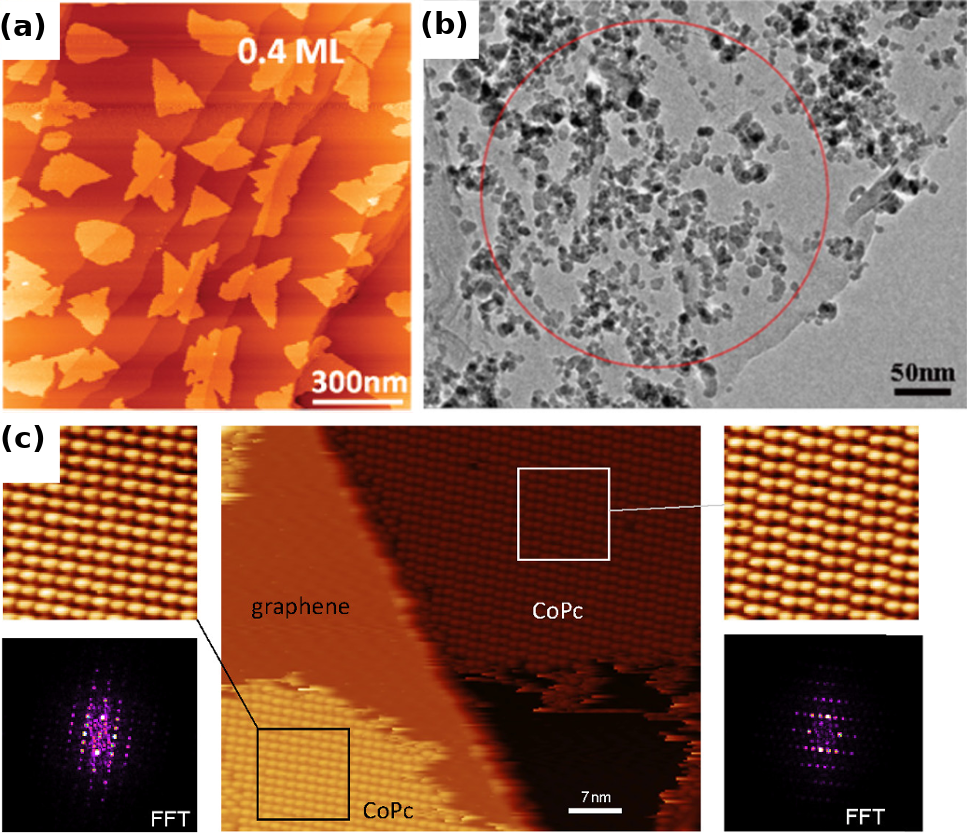
\includegraphics[width=0.8\textwidth]{Introduction/Figures/Untitled_new.png}
    \caption[Representative images depicting various types of self-assemblies formed over a graphene surface]{(a) STM image showing dentritic growth of C\textsubscript{60} islands on graphene/Ru(0001) at low coverage. Reprinted (adapted) with permission from ref.\supercite{lu_using_2012}. Copyright 2023 American Chemical Society. (b) TEM image of 10Fe-GO system. Reprinted (adapted) with permission from ref.\supercite{yang_electrostatic_2020}. Published by Elsevier B.V. on behalf of Cairo University. (c) STM image (0.7V/2pA) showing two CoPc islands with kinks in different directions of the CoPc lattice. Reprinted (adapted) with permission from ref.\supercite{hamalainen_self-assembly_2012}. Copyright 2023 American Chemical Society.}
    \label{fig:figure1}
\end{figure}

We briefly illustrate each of the interactions with salient examples. Molecules which are devoid of H-bonding groups or ionic groups and contain only hydrophobic cores self assemble over the graphene surface by hydrophobic driven interactions. An example of this is the self assembly of fullerene (C60) over the graphene surface. Loh and coworkers employed STM imaging to investigate the self-assembly of C\textsubscript{60} over a graphene/Ru(0001) substrate.\supercite{lu_using_2012} They chose graphene/Ru(0001) substrate due to the formation of corrugated structures, which could then influence the formation of C\textsubscript{60} self-assemblies. At low surface coverage, they observed that the C\textsubscript{60} molecules would preferentially occupy the C\textsubscript{hcp} valleys, the remaining molecules would undergo a hierarchical adsorption with the C\textsubscript{fcc} valleys getting filled next, followed by the highest points in the corrugations and finally six C\textsubscript{60} molecules would occupy the periphery of the corrugations [Figure 1.1(a)]. 

Metals and metallic nanoparticles interact with the graphene surface via electrostatic interactions. Shuai and coworkers investigated the assembly of \textit{p}-Fe\textsubscript{3}O\textsubscript{4}.\supercite{yang_electrostatic_2020}  They observed that the positively charged Fe\textsubscript{3}O\textsubscript{4} particles would form self-assemblies over the negatively charged graphene oxide (GO) via electrostatic interactions. From TEM images, they confirmed that the \textit{p}-Fe\textsubscript{3}O\textsubscript{4} nanoparticles were able to form homogeneous assemblies over GO nanosheets, in the case of 10Fe-GO system [Figure 1.1(b)]. They also observed that the electrostatic interactions between the positively charged Fe\textsubscript{3}O\textsubscript{4} particles and the negatively charged GO sheets have a synergic effect, promoting the dispersion of both the structures.

Molecules which contain a chelated metal, exhibit both electrostatic and hydrophobic interactions with the graphene sheet. Sainio and colleauges investigated the formation of self-assembled monolayers in Cobalt-Phthalocyanines over a graphene/Ir(111) substrate using STM imaging.\supercite{hamalainen_self-assembly_2012} They observed that the CoPc molecules formed a square lattice over the graphene surface [Figure 1.1(c)], even though the underlying graphene/Ir(111) moire pattern had a hexagonal symmetry. They concluded that this was due to the weak coupling between the graphene and the underlying Ir(111) surface, and opined that graphene/Ir(111) can be a suitable substrate to further investigate the formation of molecular self-assemblies.

Molecules which exhibit extended self-assembled stcutures are those which contain H-bond donor and acceptor groups. Nucleic acids are known to form extendes self assemblies on metallic surfaces like Au(111) and and Cu(111).\supercite{kelly_understanding_2008,lukas_adenine_2009,tsud_adenine_2015,otero_guanine_2005,otero_elementary_2008} Besenbacher and coworkers investiagted the formation of self-assembled monolayers in canonical nucleobases dispersed over Au(111) using STM imaging and ab-initio modelling.\supercite{kelly_understanding_2008,lukas_adenine_2009,otero_guanine_2005,otero_elementary_2008} They observed the formation of ordered networks at low surface coverages which gradually transformed towards random glassy structures with increasing surface coverages.\supercite{otero_elementary_2008}  Nucleobases are also found to form self assemblies on graphene surfaces. Multiple groups have investiagted the formation of 2D self-assemblies in nucleobases dispersed over a graphene surface.\supercite{heckl_two-dimensional_1991,freund_structure_1997,xu_coadsorption_2006,akinwande_large-area_2015,spada_guanosine-based_2008,mamdouh_supramolecular_2006} Heckl and colleagues investigated the formation of 2D networks in adenine molecules dispersed over a graphite surface using STM imaging and Low Energy Electron Diffraction (LEED) experiments.\supercite{heckl_two-dimensional_1991} Similar studies were performed for other nucleobases and (or) nucleobase derivatives.\supercite{freund_structure_1997,xu_coadsorption_2006,mamdouh_self-assembly_2009,wang_controlling_2014,mu_temperature-dependent_2013} The adsorption of nucleobases on the graphene surface is mediated by $\pi-\pi$ interactions, and the preferred orientation of the adsorbent molecule is to align parallel to the underlying graphene surface in order to maximize the $\pi-\pi$ interactions between them. The adsorbent molecules also prefer a ‘AB’ type stacking with respect the underlying graphene lattice, where the face of the adsorbent molecule is slightly shifted from the graphene lattice.

In addition to the self assembly of nucleobases on graphene polymeric DNA strands are also know to adsorb and undergo 2D diffusion over graphene surfaces.\supercite{hampitak_protein_2020,wei_control_2019,he_planar_2020,shankla_step-defect_2019,shankla_conformational_2014,wells_assessing_2012} One of the unique features of multilayer graphene is the interlayer spacing of $\approx$ 3.4 $\angstrom$. This matches the distance between subsequent nucelobases (rise) observed in DNA. These features attracted the exploration of graphene based solid state nanopores for sequencing DNA. In 2010, three groups independently demonstrated the applicability of graphene membranes as suitable tools to detect DNA translocations.\supercite{merchant_dna_2010,schneider_dna_2010,garaj_graphene_2010} They were able to drive the DNA strand through a nanopore constructed in the graphene membrane, and used blockades in the ionic current flowing across the membrane to identify the translocation of DNA strands. This indicated the possibility of employing graphene-based solid-state devices to sequence DNA strands. Solid-state nanopores, such as those constructed in graphene, can sequence long single-stranded DNA molecules without requiring strand fragmentation.\supercite{merchant_dna_2010,schneider_dna_2010,garaj_graphene_2010,li_dna_2003,yuan_solid-state_2018,xue_solid-state_2020} The fragmentation of the full DNA into overlapping short segments is a required step in traditional Sanger-based methods used in many next-generation sequencing methods, and it is a common source of error in reconstructing the complete DNA sequence.\supercite{sanger_dna_1977,daniels_sanger_2021,curci_how_2015} Therefore, it is imperative that a clear understanding of the dynamics of DNA strands near graphene nanopores is required to design graphene membranes with specific properties for DNA sequencing.\supercite{schneider_tailoring_2013} As a first step towards that, it is critical to understand the interactions between the nucleobases, nucleosides, and nucleotides and the graphene surfaces.

Here, we summarize the experimental and theoretical studies describing the interaction of nucleic acids, both as an individual nucelobase and as a polymer, with graphene. We categorize the results in two broad areas: (a) Graphene as a two-dimensional solid support for nucleobase-assisted self-assemblies and (b) Graphene based nanopores as a reliable tool for rapid sequencing of DNA. 

The Introduction is organized in the following order:
\begin{itemize}
    \item We first discuss the studies describing the binding energetics of monomeric nucelobases or polymeric DNA strands interacting with the graphene surface.
    \item We then focus on the formation of nucleobase self-assemblies over a graphene surface.
    \item In the final section, we review the studies utilizing graphene-based devices for sequencing single-stranded DNA (ssDNA) and double-stranded DNA (dsDNA).
\end{itemize} 

In all the sections we discuss results from both the experimental and theoretical standpoints.

\section{Energetics of Interactions with Graphene surface}
The interaction between the nucleobases and the graphene surface has been investigated in the literature via both experimental and computational studies. Experimentally, Isothermal calorimetry (ITC)  experiments and single-molecular force spectroscopy (SMFS) are employed to investigate the binding of nucleobases and (or) short ssDNA strands with the graphene surface. Theoretically, ab-initio calculations and molecular dynamics simulations are used to investigate binding energies. ab-initio calculations are performed in the gas-phase while molecular dynamics simulations are used to study the binding energetics in aqueous phase. 

To understand the process of self-assembly of nucleobases on the graphene surface and the translocation dynamics of DNA strands through the nanopore, it is important to gain insights into the binding energetics of nucleobase-graphene interactions. Here, we review a few critical experimental and computational studies investigating the vdW interactions between the nucleobases (small DNA strands) with the graphene surface.

\subsection{Nucleobases}
\subsubsection{Experimental Studies}
\paragraph{Isothermal calorimetry:} Rao and coworkers investigated the binding free energies of four canonical DNA nucleobases with the graphene surface using isothermal calorimetry (ITC) experiments in aqueous and basic environments.\supercite{varghese_binding_2009} They obtained interaction energies of -6.64 (-11.85), -- (-13.45), -4.39 (-9.38) and -0.68 (-4.72) kcal/mol for adenine, guanine, cytosine and thymine in aqueous (basic) environments. The binding free energies follow the relative ordering of guanine $>$ adenine $>$ cytosine $>$ thymine, with significantly stronger interactions with the graphene surface being observed in basic media compared to aqueous media. This trend also revealed stronger binding for purines (adenine, guanine) when compared to pyrimidines (cytosine, thymine).

\subsubsection{Computational Studies}
\begin{figure}
    \centering
    \includegraphics{Introduction/Figures/Figure2.png}
    \caption[Equilibrium geometry of nucleobases on top of graphene: (a) guanine, (b) adenine, (c) thymine, (d) cytosine, and (e) uracil from ab-initio calculations]{Equilibrium geometry of nucleobases on top of graphene: (a) guanine, (b) adenine, (c) thymine, (d) cytosine, and (e) uracil. Reprinted (adapted) with permission from ref.\supercite{gowtham_physisorption_2007} Copyright 2023 American Physical Society.}
    \label{fig:figure2}
\end{figure}

\paragraph{ab-initio studies:} ab-inito DFT calculations generally employ the following scheme to obtain the binding energies and minima, where a routine geometry optimization is performed for the combined nucleobase - graphene model system, and the binding energies are then obtained as the difference between the energy of the nucleobase - graphene system and the sum of individual molecules (graphene sheet and nucleobase).

Karna and coworkers investigated the various factors influencing the physisorption of nucleobases over the graphene surface.\supercite{gowtham_physisorption_2007} They employed periodic density functional theory (DFT) and single molecule calculations at M\"{o}ller-Plusset (MP2) level of theory and split-valence 6-311++G(d,p) basis set to investigate the relevant descriptors. They observed that interaction energies were dependent on the orientation of the nucleobases with respect to the graphene surface, with parallel stacking of nucleobases being the most stable configuration [Figure 1.2]. They also observed that the presence of heteroatoms (nitrogen and oxygen) on the nucleobases affects the interactions between the nucleobases and the graphene surface. The binding energies for adenine, guanine, cytosine, thymine and uracil were found to be -21.68, -24.68, -18.45, -19.14 and -17.06 kcal/mol, respectively. A strong dependence of the molecular polarizability of the nucleobases on the stabilization of the inter-molecular interactions was also observed, with guanine having the highest molecular polarizability and uracil having the lowest molecular polarizability.

Grimme and coworkers investigated the energetics of $\pi$-stacked graphene nucleobase complexes.\supercite{antony_structures_2008} They employed DFT calculations at B97-D functional and a triple-zeta valence plus polarization TZV(2d,2p) basis set to investigate the relevant properties of the complexes (interaction energies, geometries and electronic properties). The interaction energies were found to be strongly dependent on the stacking geometry. The most stable configuration was observed to be the parallel stacked configuration, which maximized the $\pi$-stacking interactions between the graphene surface and the nucleobase. The binding energies for adenine, guanine, cytosine, thymine and uracil were calculated to be -20.6, -26.3, -19.2, -19.9 and -17.0 kcal/mol, respectively. They also observed that the interactions between the graphene surface and the nucleobases were primarily mediated via dispersion interactions, with the interaction energies showing a direct relationship with the number of carbon atoms included in the graphene unit cell.

\begin{figure}
    \centering
    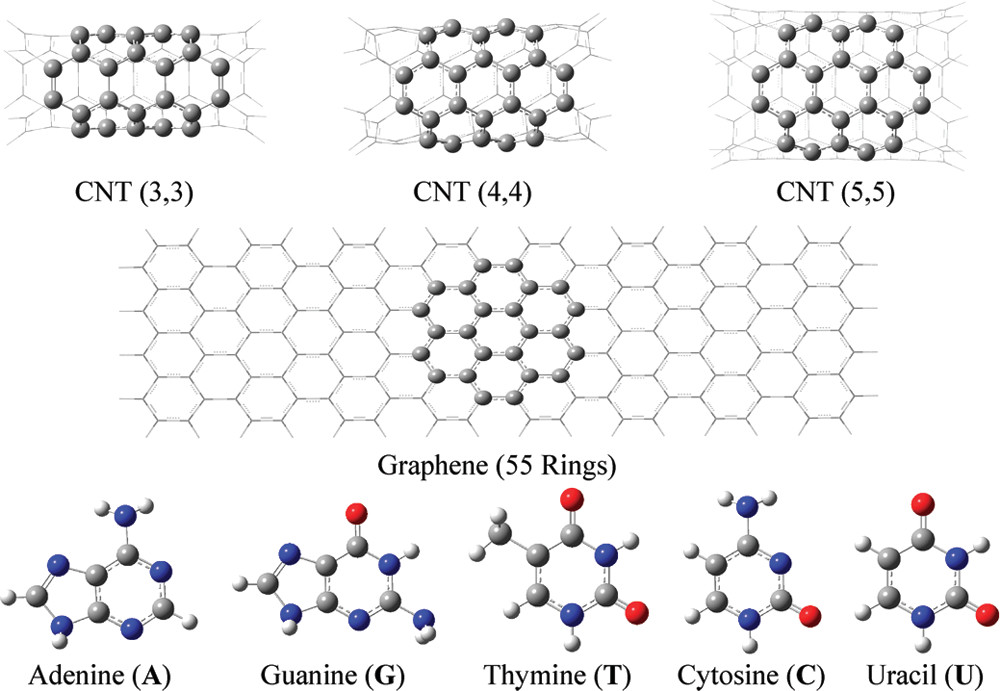
\includegraphics{Introduction/Figures/Figure3.png}
    \caption[Representative structures corresponding to (3,3), (4,4), (5,5) SWCNTs, graphene sheet and canonical nucleobases]{Representative structures corresponding to (3,3), (4,4), (5,5) SWCNTs, graphene sheet and canonical nucleobases are also presented. Atoms considered interacting in ONIOM are depicted as balls and sticks, and other atoms are depicted as lines. Figure adapted from scheme presented in ref \supercite{umadevi_quantum_2011}. Copyright 2023 American Chemical Society.}
    \label{fig:figure3}
\end{figure}

Using single-molecule DFT calculations, Sastry and coworkers investigated the interactions of nucleobases with a poly-conjugated surface and carbon nanotubes.\supercite{umadevi_quantum_2011} They investigated the binding energies of nucleobases with four sets of surfaces: a flat graphene surface and three carbon nanotubes of increasing radii starting from (3,3) to (5,5) as shown in Figure 1.3. The ONIOM formalism with M06-2x Minnesota functional and 6-31g* basis was used to describe atoms in the QM layer, and AM1 semi-emperical method was used to describe other atoms. The central coronene ring section of the graphene sheet and the nucleobases were marked as QM layer, and the remaining atoms were assigned to semi-empirical layer. The binding energies for nucleobases interacting with the graphene surface were found to be -14.14, -14.78, -13.30, -14.29 and -11.92 kcal/mol for adenine, guanine, cytosine, thymine and uracil, respectively. The nucleobases' binding energies were found to be strongly dependent on the curvature of the surface, with the highest binding energies obtained when the surface is devoid of curvature. This observation was ascribed to the increase in the $\pi$-stacking interactions between the nucleobase and the adsorbent surface as the curvature of the adsorbent decreases.

Kim and coworkers investigated the binding of nucleobases with two systems: naphthalene and a graphene surface (modelled as an n=5 flake with 150 carbons arranged in hexagonal symmetry).\supercite{cho_noncovalent_2013} The authors obtained interaction energies of -19.8, -21.7, -18.4 and -19.7 kcal/mol for adenine, guanine, cytosine and thymine, respectively using periodic DFT calculations at the semilocal Perdew–Burke–Ernzerhof (PBE) functional coupled with the pairwise Tkatchenko-Scheffler (TS) dispersion correction. The binding free energies obtained by Kim and coworkers were comparable to the values obtained by Karna et al.\supercite{gowtham_physisorption_2007} and Grimme et al.\supercite{antony_structures_2008} while differing in the computational methods adopted.

Cho and coworkers investigated the interaction between nucleobases and graphene surface using multiple functionals (LDA, PBE, PBE+vdW and vdW-DF) and observed that guanine had the strongest binding across all nucleobases, while cytosine was the weakest.\supercite{lee_physisorption_2013} The authors obtained binding energies of -23.06 (-14.53), -27.31 (-17.06),  -21.45 (-13.38) and  -21.91 (-13.84) kcal/mol for adenine, guanine, cytosine and thymine, respectively from PBE+vdW (vdW-DF) calculations. They also observed that the the main contribution to the vdW interactions between the nucleobases and the graphene surface arose from the $\pi$-orbitals belonging to the substrate and the nucleobase.

The calculations all indicate towards a very strong $\pi$-$\pi$ interaction between the nucleobase and the graphene surface, with the face of the nucleobase lying almost flat on the surface.\supercite{cho_noncovalent_2013,antony_structures_2008,umadevi_quantum_2011,vovusha_adsorption_2015,bhai_probing_2020,lee_physisorption_2013,le_physisorption_2012,panigrahi_interaction_2012,cortes-arriagada_intermolecular_2021,cortes-arriagada_phosphorene_2018} It also emerges that the binding energies follow the trend guanine $>$ adenine $>$ thymine $>$ cytosine, irrespective of the method used for the calculation. ab-initio methods are generally employed to investigate the interaction of only one nucleobase with a graphene sheet or patch of graphene in a gas phase environment. However, experimental studies are carried out in an aqueous (or basic) environment. Thus an accurate description of the binding characteristics would require the explicit inclusion of water molecules. Molecular Dynamics simulations offer a suitable framework to investigate the effect of solvation on the binding characteristics of nucleobases with the graphene surface.

\paragraph{Molecular Dynamics Simulations:} Molecular Dynamics (MD) simulations generally employ a metadynamics pathway for the investigation of such binding energies, where a particular reaction coordinate, generally denoted as $\zeta$ (the z-projected distance between the nucleobase and the graphene surface in this case) is scanned in an MD simulation via the application of a biasing force.

Walsh and coworkers investigated the binding of nucleobases with the (0001) surface of HOPG using metadynamics simulations.\supercite{hughes_adsorption_2017} They obtained binding energies of -5.38 $\pm$ 0.24, -6.62 $\pm$ 0.38, -3.08 $\pm$ 0.21 and  -3.94 $\pm$ 0.24 kcal/mol for adenine, guanine, cytosine and thymine respectively. It is interesting to note that the relative ordering of the interaction energies remains consistent with the ab-inito calculations, which also predicted an ordering of guanine $>$ adenine $>$ thymine $>$ cytosine. The metadynamics simulations also predicted the first minima at $\sim$ 3.8 $\angstrom$, indicative of the strong $\pi$-$\pi$ interactions between the nucleobases and the graphene surface.

\begin{table}
    \centering
    \caption[Binding free energies (in kcal/mol) of nucleobases interacting with the graphene surface]{Binding free energies (in kcal/mol) of nucleobases interacting with the graphene surface. Experimental values are compared with those obtained from quantum mechanical (QM) calculations and Additive non-polarizable simulations. Exp. = aqueous solution and Exp.\textsuperscript{\#} = NaOH (basic) solution. QM\textsuperscript{\#} = MP2/6-311++ G(d,p), QM\textsuperscript{$\dag$} = B97-D/TZV(2d,2p), QM\textsuperscript{$\ddag$} = ONIOM (M06-2X/6-31G*:AM1) and QM\textsuperscript{*} = vdW-DF
    }
    \label{tbl:example1}
    \begin{tabular}{@{}cccccccc@{}}
        \toprule
        System & Exp.\supercite{varghese_binding_2009} & Exp.\textsuperscript{\#}\supercite{varghese_binding_2009} & QM\textsuperscript{\#}\supercite{gowtham_physisorption_2007} & QM\textsuperscript{$\dag$}\supercite{antony_structures_2008} & QM\textsuperscript{$\ddag$}\supercite{umadevi_quantum_2011} & QM\textsuperscript{*}\supercite{cho_noncovalent_2013} & add. \supercite{hughes_adsorption_2017} \\ \midrule
        Adenine & -6.64 & -11.85 & -21.68 & -20.6 & -14.14 & -14.53 & -5.38 \\
        Guanine & -- & -13.45 & -24.68 & -26.3 & -14.78 & -17.06 & -6.62 \\
        Cytosine & -4.39 & -9.38 & -18.45 & -19.2 & -13.30 & -13.38 & -3.08 \\
        Thymine & -0.68 & -4.72 & -19.14 & -19.9 & -14.29 & -13.84 & -3.94 \\
        Uracil & -- & -- & -17.06 & -17.0 & -11.92 & -- & -- \\ \bottomrule
        \end{tabular}
    \end{table}    

% Inspired by the ab-initio calculations\supercite{gowtham_physisorption_2007,antony_structures_2008,umadevi_quantum_2011,cho_noncovalent_2013}, we investigated the effect of molecular polarizability on the adsorption of nucleobases over a graphene surface.\supercite{h_polarization_2021} We demonstrated the the inclusion of polarizability plays an important role in determining the energetics of the interactions between the nucleobases and the graphene surface. The binding energies from classical Drude polarizable FF simulations for adenine, guanine, cytosine, thymine and uracil were found to be -8.35, -9.85, -5.96, -7.66 and -7.03 kcal/mol, respectively. From non-polarizable additive FF simulations, we obtained binding energies of -9.40, -9.68, -7.03, -7.97 and -7.35 kcal/mol for adenine, guanine, cytosine, thymine and uracil respectively.
  
In Table 1, we tabulate the binding free energies obtained from various experimental and theoretical studies. We note that the binding energies obtained by the multiple groups are in qualitative agreement, with the discrepancies in the actual energies arising from their specific system geometry and investigation techniques. All the results indicate that guanine has the strongest binding affinity with the graphene surface, and uracil has the weakest binding affinity across all nucleobases. From ab-intio DFT calculations and MD simulations, it is also observed that parallel stacking of the nucleobases is the most stable conformation adopted for nucleobase-graphene interactions. The inclusion of explicit solvation in the MD simulations improves the agreement between calculated binding energies and experimentally derived binding energies, an effect missing from the gas-phase QM calculations. 

\subsection{DNA strands}
\subsubsection{Experimental Studies}
\paragraph{Isothermal Calorimetry:} Chen and coworkers investigated the binding of nucleosides (adenosine, guanosine, cytidine and thymidine) and small oliginucleotides (A\textsubscript{5}, C\textsubscript{5}, AGCTA and T\textsubscript{5}) with the graphene oxide surface using isothermal calorimetry experiments.\supercite{ranganathan_complex_2016} They obtained binding free energies in the range of -30 to -37 kcal/mol for the small oligonucleotides, while a binding free energy of -6.0, -6.2, -5.8 and -5.1 kcal/mol were obtained for adenosine. guanosine, cytidine and thymidine respectively. The authors obtained a relative ordering of C\textsubscript{5} $\sim$ A\textsubscript{5} $>$ AGCTA $>$ T\textsubscript{5} for the association constants. Association constants for G\textsubscript{5} could not be obtained due to strong intermolecular interactions between the guanine nucleobases.

\paragraph{Single-Molecule Force Spectroscopy:} Vezenov and coworkers employed single-molecule force spectroscopy (SMFS) experiments to investigate the binding kinetics of short ssDNA homopolymers with the graphene surface.\supercite{manohar_peeling_2008,iliafar_quantifying_2012} They obtained the binding energies of -5.87, -4.92, -4.48 and -6.70 kcal/mol for dA\textsubscript{50}, dG\textsubscript{100}, dC\textsubscript{50} and dT\textsubscript{50} strands, respectively. It is interesting to note that they obtained the highest binding energy for thymine.  This is in contrast to the experimental and computational (ab-initio and MD) studies on the binding of nucleobases which predict the tend to be guanine $>$ adenine $>$ cytosine $>$ thymine. The authors reasoned that the formation of higher-order structures within the long ssDNA used in the experiment would play a significant role in determining the binding energies and might explain the observed discrepancy between the experimental and theoretical interaction patterns.

This observation was corroborated by the experimental investigations of Walsh and coworkers, who investigated the binding of shorter ssDNA strands (30 nucleotides long) with graphene surfaces using SMFS. The binding energies for dA\textsubscript{30}, dG\textsubscript{30}, dC\textsubscript{30} and dT\textsubscript{30} strands were found to be -9.0, -12.67, -7.65 and -7.89 kcal/mol \supercite{hughes_adsorption_2017}. The trend dG\textsubscript{30} $>$ dA\textsubscript{30} $>$ dT\textsubscript{30} $\sim$ dC\textsubscript{30} is in agreement with the trends predicted by previous experimental and computational investigations.

\begin{figure}
    \centering
    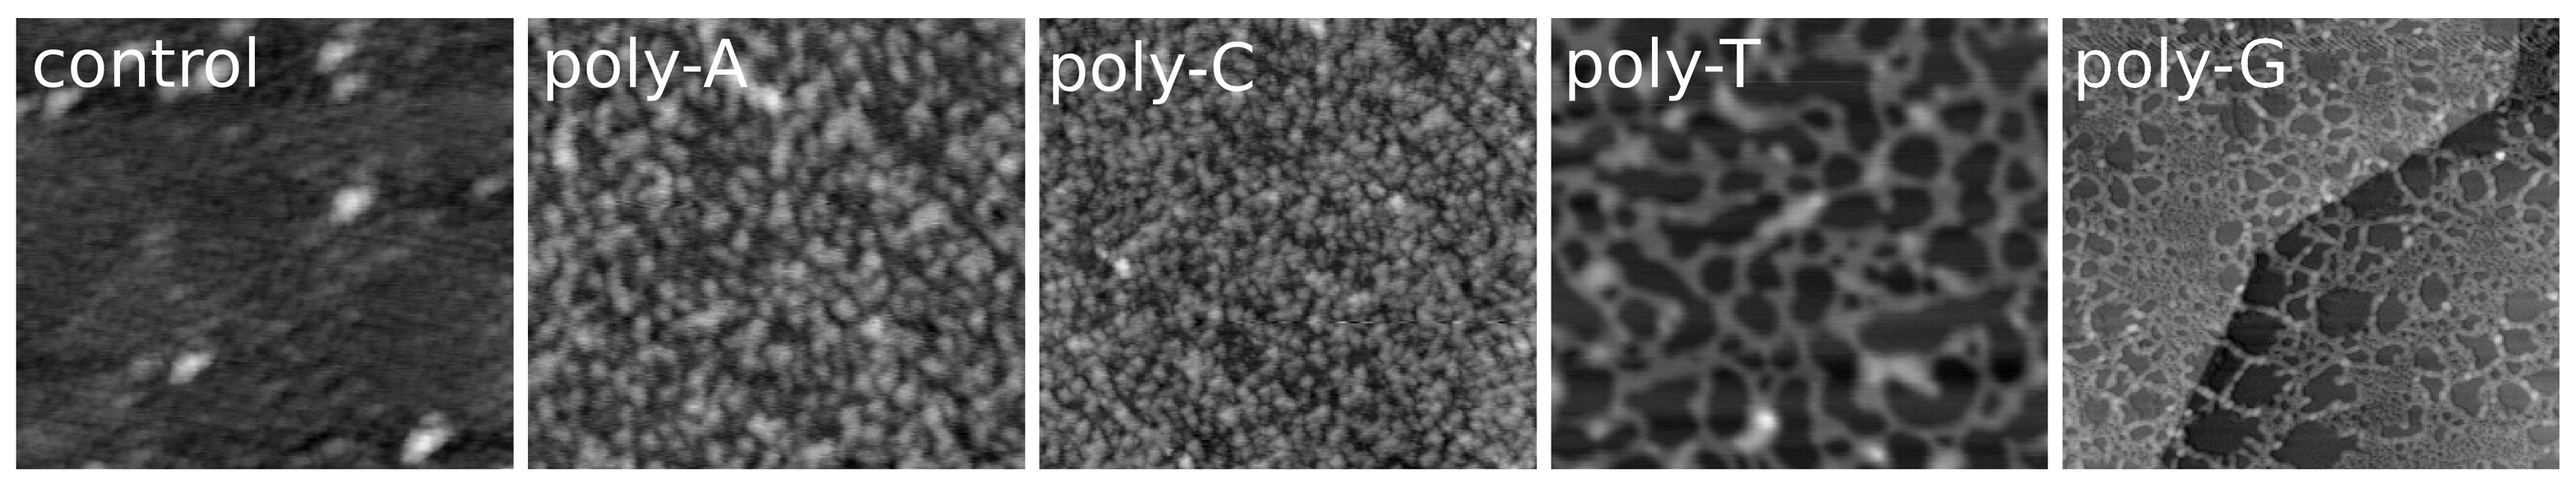
\includegraphics[width=\textwidth]{Introduction/Figures/Figure12_crop.png}
    \caption[Atomic Force Micrographs of the height of the control experiment, poly-A, C, T, and G, respectively.]{Atomic Force Micrographs of the height of the control experiment, poly-A, C, T, and G, respectively. All images are 750×750 $nm^2$, except for poly-G, which is 5×5 $\mu m^2$. Reprinted (adapted) from ref. \supercite{akca_competing_2011}. Published by Public Library of Science (PLOS).}
    \label{fig:figure4}
\end{figure}

\paragraph{Atomic Force Microscopy:}Postma and coworkers investigated the binding of ssDNA with the graphene surface using AFM imaging, in an attempt to shed light on the various competing interactions within the system.\supercite{akca_competing_2011} They observed that ssDNA would self-assemble into two distinct shapes: either into spherical particles, or into elongated chains. They also noted that poly-A and poly-C preferentially formed spherical particles, while poly-G and poly-T strands formed elongated chains while adsorbing onto the graphene surface [Figure 1.4]. They reason that the observed differences can be explained by considering two energy terms: intermolecular interactions, denoted as $E_b$ and interactions with graphene, denoted as $E_g$, with spherical particles preferred when $E_b > E_g$ and elongated chains, when $E_b < E_g$. They observed that the cross over between the spherical and extended structures is between 6.91 - 11.53 kcal/mol.

\subsection{Computational Studies}
\paragraph{Molecular Dynamics Simulations:} Liu and coworkers investigated the binding of poly-adenine, poly-thymine and poly-cytosine ssDNAs with graphene oxide surface using MD simulations.\supercite{lopez_polycytosine_2021} The most stable interactions were observed when poly-cytosine ssDNA was interacting with the GO surface, followed by poly-thymine and poly-adenine respectively. From energy calculations, they noted that the hydrogen bonding interactions between the phosphate backbone and the graphene oxide surface leads to the observed stabilization of poly-dC over the GO surface. They opined that the increased stabilization had its origins in the lack of $\pi$-stakcing interactions between the cytosine nucleobases and GO surface, leading to a significantly more flexible structure, which favoured the formation of more hydrogen bonding interactions with the GO surface. They observed that the interactions between the ssDNA and the graphene oxide surface was dependent on the pH of the solution, with basic or neutral pH favouring the binding.

Dutta and coworkers employed all-atom MD simulations to investigate the binding of ssDNA and dsDNA strands with the graphene, \textit{h}-BN and C\textsubscript{2}N surface\supercite{mukhopadhyay_screening_2020}. They employed 5-d(ATGCATGCATGC)-3 as a model sequence for ssDNA and 5-d(CGCGAATTCGCG)-3` as a model sequence for dsDNA. From MD simulations, the authors observed that the adsorption of ssDNA onto the graphene and \textit{h}-BN surfaces was a rapid process, with the intra-strand hydrogen bonds being lost within the first 200 and 100 ns of the simulation time, respectively. They estimated a binding free energy of $\sim$ -225 kcal/mol for ssDNA interacting with the graphene surface. In contrast, a much higher value of -320 kcal/mol was obtained for ssDNA interacting with \textit{h}-BN surface. For dsDNA, they observed that the adsorption of the strand was initiated by the interaction of a pair of terminal nucleobases with the surface via $\pi$–$\pi$ interactions. Similar to ssDNA, they observed a strong binding for the dsDNA with graphene and \textit{h}-BN surfaces, with binding energies of $\sim$ -385 kcal/mol for dsDNA interacting with \textit{h}-BN and $\sim$ -380 kcal/mol for dsDNA interacting with graphene surface. They noted a loss in the secondary structure of the dsDNA strand upon interacting with graphene and \textit{h}-BN surfaces, where a continuous loss of inter-strand hydrogen bonds and intra-strand $\pi$-$\pi$ interactions was observed. This loss had been ascribed to the stabilization provided by the $\pi$-$\pi$ interactions between the nucleobases and the graphene (\textit{h}-BN) surface. 

Lei and coworkers investigated the binding of ssDNA with a graphene oxide surface using MD simulations.\supercite{xu_dynamic_2017} They observed that the interactions between the ssDNA and the graphene oxide surface is mediated via both hydrogen bonding interactions between the oxidized regions of the surface and $\pi$-$\pi$ stacking interactions between the nucleobases and the unoxidized regions of the surface.

Zhao and coworkers investigated the self-assembly of ssDNA with graphene surface using molecular dynamics simulations.\supercite{cheng_steered_2012} They observed that the nucleobases in the ssDNA underwent $\pi$-$\pi$ interactions with the graphene surface, with the bases aligning parallel to the underlying surface. The relative ordering of the obtained binding energies (in kcal/mol) were found to be consistent with the results obtained from previous ab-initio calculations, with G (-18.5) $>$ A (-17.4) $>$ T (-15.4) $>$ C (-14.4).

After discussing the energetics of nucleobase binding to the graphene surface, we next discuss the process of nucelobase self-assembly on graphene support.

\section{Nucleobase Self-Assemblies}
\subsection{Homogeneous Systems}
\subsubsection{Experimental Studies}
\paragraph{Adenine:} 
Heckl and coworkers investigated the formation of 2D networks among adenine nucleobases dispersed over a graphite surface using STM imaging and Low Energy Electron Diffraction (LEED) experiments.\supercite{freund_structure_1997} From STM imaging and LEED data, they identified three distinct orientations of the adenine molecules in the observed 2D network. From all-atom MD simulations, they identified one model structure obeying the symmetry constraints imposed by the STM and LEED data. They identified an extended hydrogen-bonded network, with four hydrogen bonds per nucleobase, and the extended network of NH\textsubscript{2}-N hydrogen bonds stabilising the overall hydrogen-bonded network [Figure 1.5(a)]. They also observed that the adsorbed molecules were not perfectly flat over the graphene surface, with a slight tilt with respect to the normal vector to the graphene surface.

\begin{figure}
    \centering
    \includegraphics[width=\textwidth]{Introduction/Figures/Figure4.png}
    \caption[Representative structures for adenine self-assemblies over graphene]{(a) STM image of an epitaxially grown monolayer of adenine on graphite (001) with molecule positions indicated (size of the imaged area: 48$\angstrom$*32$\angstrom$; U = 1.0 V, I = 90 pA, constant current mode). (b) High-resolution STM constant-current image of alkyl-substituted adenine (A-C20) physisorbed onto a graphite surface from 1-phenyloctane solution (12.0 nm × 12.0 nm, V\textsubscript{bias} = 0.6 V, I\textsubscript{set} = 0.7 nA). (c) Model suggestion to characterize the packing in the STM image of panel b. (d) High-resolution STM constant-current image of A-C20 physisorbed onto a graphite surface from 1-phenyloctane solution (15.0 nm × 15.0 nm, V\textsubscript{bias} = 0.7 V, I\textsubscript{set} = 0.8 nA). (e) Model suggestion to characterize the packing in the STM image of panel d. Panel a is reprinted (figure) with permission from \supercite{freund_structure_1997}. Copyright 2023 by the American Physical Society. Panels b-e is Reprinted (adapted) with permission from ref \supercite{mu_temperature-dependent_2013}. Copyright 2023 American Chemical Society. }
    \label{fig:figure5}
\end{figure}

Chi and coworkers investigated the self-assembly of a long alkyl-chain (icosane) terminated adenine derivative on a HOPG surface as a function of temperature.\supercite{mu_temperature-dependent_2013} They employed in-situ STM imaging and ab-initio DFT calculations to characterize the self-assemblies. Two distinct forms ($\alpha$- and $\beta$-) of the self-assembly were observed depending on the temperature. Interconversion between the two forms were also investigated as a function of the temperature [Figure 1.5(b-e)]. 

\paragraph{Guanine:} Spada and coworkers investigated the formation of self-assemblies in guanosine derivatives dipersed over an HOPG surface using STM imaging\supercite{gottarelli_self-assembly_2000}. They observed that the side chains (\textit{p}-(C\textsubscript{12}H\textsubscript{25}O)C\textsubscript{6}H\textsubscript{4} and C\textsubscript{9}H\textsubscript{19}) remained flat on the graphene surface, and the self-assembled mono-layer consisted of two ribbon-like arrangements of guanine molecules interacting via hydrogen bonds.

Samor\`{i} and coworkers demonstrated the formation of self-assembled monolayers of N$^9$-substituted guanine molecules over a HOPG surface using STM imaging and ab-initio DFT calculations.\supercite{ciesielski_nanopatterning_2010} They investigated the effect of side chain length on observed self-assemblies at the HOPG - 1,2,4-trichlorobenzene interface. The authors observed the formation of distinct self-assemblies for varying side chain lengths, with the smallest alkyl chain molecule adopting a ribbon-like structure. In contrast, the larger ones progressively moved towards crystalline structures, stabilized via hydrogen bonding interactions.

\begin{figure}
    \centering
    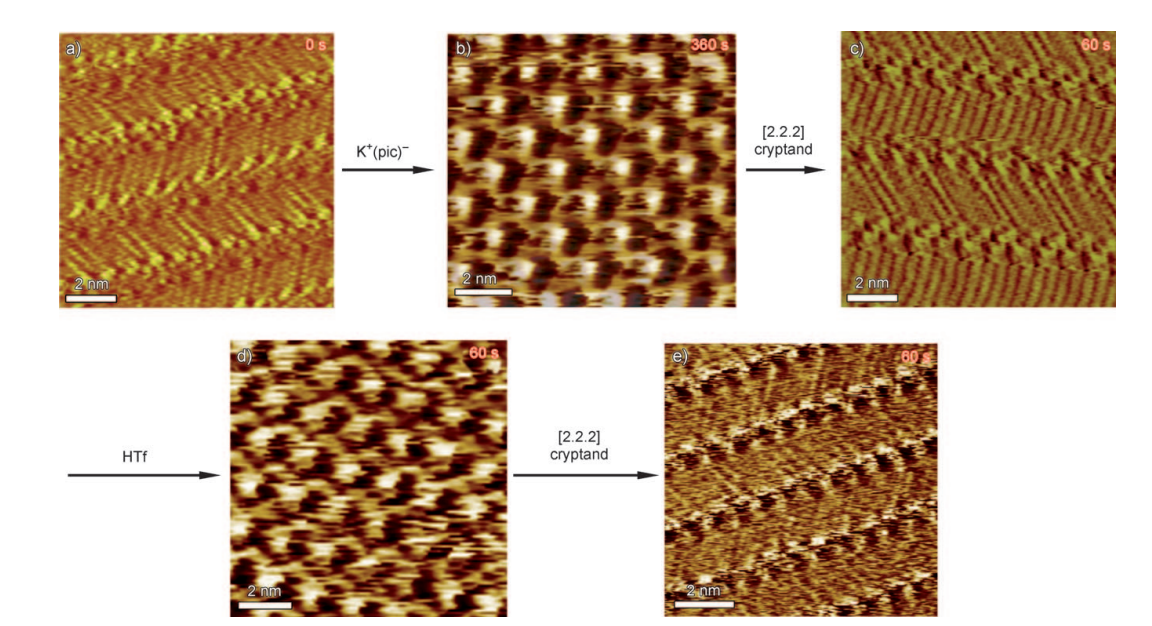
\includegraphics[width=\textwidth]{Introduction/Figures/Figure5.png}
    \caption[STM images demonstrating the structural evolution of monolayer of guanosine derivatives over graphene surface]{Consecutive STM images showing the structural evolution of a monolayer of guanosine derivatives over a 9 min time scale (time range displays in the upper right part of the images correspond to the time that was needed to reach the equilibrium after addition of reacting agents). (a), (c), and (e) show ribbon-like structure, whereas (b) and (d) exhibit G4-based architectures. Tunneling parameters: (a), (c), and (e) U$_t$=350 mV and I$_t$=15 pA; (b) and (d) U$_t$=200 mV and I$_t$=5 pA. Figure adapted (reprinted) with permission from ref. \supercite{ciesielski_dynamers_2010}. Copyright 2023 John Wiley and Sons.}
    \label{fig:figure6}
\end{figure}

Samor\`{i} and coworkers demonstrated the inter-conversion between a ribbon-like guanine supramolecular structure and G4 quartets in N$^9$-alkylguanine molecules dispersed over a graphite surface\supercite{ciesielski_dynamers_2010}. They demonstrated that the structures can be inter-converted with the addition of potassium picrate, [2.2.2]cryptand and trifluromethanesulfonic acid (HTf), where the addition of potassium ions drives the conversion towards G4 quartets, and the addition of cryptand facilitating the back-conversion to ribbon-like structures. They were able to demonstrate the successive interconversions via STM imaging, where the observed transitions in the monolayer corresponded to the two states [Figure 1.6].

Li and coworkers investigated the formation of 2D self-assembled monolayers in guanine molecules dispersed over an HOPG surface using STM imaging\supercite{xu_directional_2021}. They observed that the guanine molecules self-assembled into two distinct strcutures, one resembling a linear structure, and other corresponding to a G4 quartet. They observed that the guanine quartets are connected via intermolecular hydrogen bonds, extending the observed 2D network into a line.

We note that multiple reports of guanosine-based self-assemblies are available in the literature\supercite{spada_guanosine-based_2008,xu_directional_2021,ciesielski_dynamers_2010,ciesielski_nanopatterning_2010,gottarelli_self-assembly_2000}, and the results seem to agree that the guanine molecules tend to self-assemble into one of the three forms: either into linear chains of guanine molecules, or into G4 quartets, or into a combination of these two forms. 

\begin{figure}[h]
    \centering
    \includegraphics[width=\textwidth]{Introduction/Figures/figure_cytosine.png}
    \caption[STM images for cytosine self-assemblies over graphene]{(a) STM image of pure cytosine at water-HOPG interface (20*20  nm\textsuperscript{2};  scale bar, 5 nm; imaging tunneling current, 561.7 pA; tunneling bias, 770.3 mV). (b) Correlation-averaged zoom-in (5*5nm\textsuperscript{2}; scale bar, 1 nm). A unit cell is indicated. Reprinted (adpated) with permission from ref.\supercite{xu_coadsorption_2006}. Copyright 2023 American Chemical Society. (c) Atom numbering in cytosine molecule. (d) STM image depicting the self-assembled networks formed by cytosine molecules at the water–HOPG interface (I = 0.74nA and V = -0.42 V). High-resolution STM images show (e) self-assembled networks formed by cytosine molecules (I = 0.78nA, V = -0.45 V). Panel (d-e) adapted (reprinted) with permission from ref.\supercite{xu_directional_2021}. Copyright 2023 Elsevier.}
    \label{fig:figure7}
\end{figure}

\paragraph{Cytosine:} Besenbacher and coworkers investigated the formation of 2D self-assembled monolayers dispersed over an HOPG surface using STM imaging and DFT calculations\supercite{xu_coadsorption_2006}. They observed that cytosine molecules self-assembled in linear chains of cytosine molecules interacting via intermolecular hydrogen bonding interactions [Figure 1.7(a-b)]. From SCC-DFTB calculations, they identified that the 1D cytosine chain were formed from cytosine dimers interacting via symmetric hydrogen bonds between C2(O) and N1 atoms. We present the atom numbering used in Figure 1.7(c).

Li and coworkers also investigated the formation of 2D self-assembled monolayes in cytosine molecules disperesed over an HOPG surface using STM imaging\supercite{xu_directional_2021}. They observed the formation of an ordered 2D self-assembled structure composed of parallel 1D chains, where individual cytosine molecules form four hydrogen bonds with two neighbors, forming a chainlike structure [Figure 1.7(d-e)].

\paragraph{Thymine:} Besenbacher and coworkers investigated the formation of supramolecular self-assemblies at the interface of HOPG and 1-octanol for thymine nucleobases using STM imaging\supercite{mamdouh_supramolecular_2006}. They observed the formation of 1D chains of interacting thymine molecules, where thymine dimers self-assembled into parallel chains, which were further stabilized via inter-molecular hydrogen bonding interactions. Each thymine molecule forms four hydrogen-bonds with two of its neighbors in a chainlike structure, resulting in a zigzag arrangement of nucleobases.

\begin{figure}
    \centering
    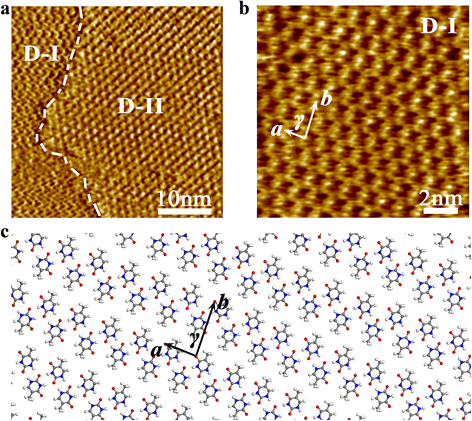
\includegraphics[width=0.5\textwidth]{Introduction/Figures/Figure17.png}
    \caption[STM images for thymine self-assemblies over graphene]{(a) STM image depicting two adjacent domains of self-assembled monolayers of melanine and thymine nucelobases over graphite surface. (b) HR-STM image for D-I domain formed by thymine molecules. V\textsubscript{bias}=0.450 V and I\textsubscript{t}=0.102 nA. (c) Proposed model structure for thymine self-assembly. Figure adapted from ref.\supercite{zhao_investigating_2016}. Published by Springer Nature.}
    \label{fig:figure8}
\end{figure}

Liu and coworkers investigated the adsorption of thymine nucleobases at 1-octanol/HOPG interface using STM imaging.\supercite{zhao_investigating_2016} They observed the formation of a zig-zag arrangement of thymine molecules, where a thymine molecule is interacting with the neighbouring molecules via intermolecular hydrogen bonding interactions, facilitated via C2(O) and N3 atoms [Figure 1.8]. This observation is in agreement with the results from Besenbacher et al., who also investigated the formation of such self-assemblies in a very similar system.\supercite{mamdouh_supramolecular_2006}

Having discussed the experimental studies of 2D self-assemblies in canonical nucleobases disperesed over a graphene and (or) HOPG surface, we now focus on the computational investigations exploring the same phenomenon. Computational studies provide atomistic insights in processes that play an important role in the formation of the observed self-assemblies. To this end, we now summarize investigations based on all-atom molecular dynamics simulations.

\subsubsection{Computational Studies}
\paragraph{Molecular Dynamics Studies:} Heckl and coworkers investiagted the self-assembly of adenine nucelobases disperesed over a graphite surface using Dreiding II FF.\supercite{edelwirth_molecular_1998} In a previous investigation, they had observed the formation of self-assembled adenine monolayers over graphite.\supercite{freund_structure_1997} From the three dimeric assemblies which were considered to model the observed self-assembly, only one dimeric assembly was found to reach convergence after energy minimization and lattice dynamics simulations. The final assembly was observed to be composed of adenine dimers interacting via hydrogen bonding interactions [Figure 1.9].
\begin{figure}
    \centering
    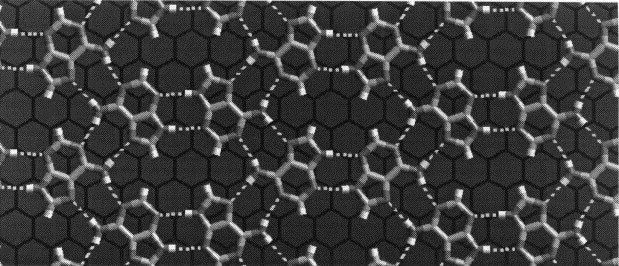
\includegraphics{Introduction/Figures/Figure18.png}
    \caption[Representaive image depicting adenine self-assemblies over graphene]{2D self-assembly of adenine nucleobases over graphite surface. Hydrogen bonds are represented using dashed lines. Figure adpated with permission from ref.\supercite{edelwirth_molecular_1998}.Copyright 2023 Elsevier Science B.V.}
    \label{fig:figure9}
\end{figure}

Dutta and coworkers investigated the energetics of the formation of 2D assemblies by guanine, xanthine and hypoxanthine nucleobases over graphene, hexagonal boron nitride (\textit{h}-BN), and black phosphorene. They observed that the nucleobases retained the quartet geometry on all the investigated surfaces at lower temperatures, while significant reorganization of the nucleobases and subsequent loss of the quartet geometry were observed at higher temperatures.\supercite{mukhopadhyay_design_2018}  The authors reported a stabilizaton of $\sim$ 30 kcal/mol for the individual nucleobases involved in the quartet formation at lower temperatures, indicating the preference for the nucleobases to self-assemble into 2D assemblies. They also observed significant inter-quartet hydrogen bonding interactions between the quartets, providing extra stabilization to the 2D self-assembly.

Pandey and coworkers investigated the dynamics of guanine and cytosine nucleobases adsorbed over a graphene surface using non-polarizable additive FF MD simulations.\supercite{saikia_hierarchical_2017, saikia_dynamics_2018} They investigated the formation of self-assembled structures in guanine and cytosine nucleobases disperesed over a graphene surface in the presence and absence of solvent. They observed a significant difference in the interaction patterns observed in gaseous and aqueous phase simulations, with gaseous phase calculations predicting the formation of self-assembled structures stabilized by inter-molecular hydrogen bonding and $\pi$-stacking interactions between the nucleobases. In contrast, aqueous phase calculations predict a dispersed state with the nucleobases primarily interacting with the underlying graphene surface via $\pi$-stacking interactions [Figure 1.10(a-c)]. The loss of inter-molecular hydrogen bonding interactions between the nucleobases in the aqueous phase calculations results in a dispersed configuration. However, their observation was in starck contrast to the experimental observations\supercite{mu_temperature-dependent_2013, ciesielski_self-assembly_2013, heckl_two-dimensional_1991, freund_structure_1997} where significant hydrogen bonding interactions between the nucleobases stabilized the self-assembled monolayers.

\begin{figure}[h]
    \centering
    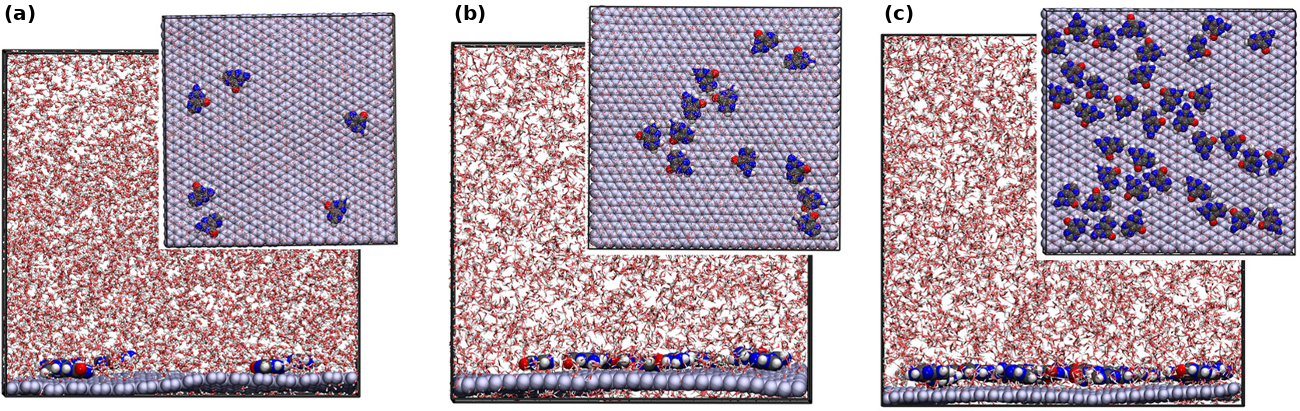
\includegraphics{Introduction/Figures/Figure7_cropped.png}
     \caption[Representaive image depicting guanine and cytosine self-assemblies over graphene]{(a–c) Snapshots of Gn bases (n = 6, 12, and 36) physisorbed on graphene in solvent.  Reprinted (adapted) with permission from ref \supercite{saikia_hierarchical_2017}. ACS.}
     \label{fig:figure10}
\end{figure}

% Previous studies based on ab-inito calculations have demonstrated that the strength of the non-covalent interactions between the nucleobases and the underlying graphene surface is proportional to the molecular polarizability of the nucleobases and the surface.\supercite{gowtham_physisorption_2007} Ab-inito calculations were also used in conjunction with experimental studies to explore how nucleobases self-assemble on a graphene (or graphite) surface.\supercite{xu_coadsorption_2006,ciesielski_nanopatterning_2010,wang_controlling_2014,mu_temperature-dependent_2013} However, due to the poor scaling of ab-initio methods, the applicability of these methods are limited to the study small molecular clusters or unit cells, indicating that they are not suitable to understand the dynamics of nucleobases on a graphene surface. In constrast, Molecular Dynamics simulations offer a much more accessible pathway towards understanding such dynamics. However, we note that additive FF simulations based on fixed point charges are ill-equipped to describe molecular polarizability, leading to errenous simulation outcomes.

% To understand the effect of molecular polarizability on the dynamics of nucleobases dispersed over a graphene surface, we investigated the dynamics of nucleobases dispersed over a graphene surface using Drude polarizable FF simulations.\supercite{h_polarization_2021} We demonstrated that the inclusion of polarizability plays a vital role in determining the dynamics of the nucleobases dispersed over the graphene surface. We observed the formation of ordered self-assembled structures by cytosine nucleobases adsorbed over a graphene surface, where strong inter-molecular hydrogen bonding interactions stabilized the self-assembled structures [Figure 1.10(d)]. The non-polarizable additive FF simulations did not account for this observation.

% In the same study, we also observed significant differences in the dynamics of guanine nucleobases disperesed over a graphene surface based on the FF that was employed. In non-polarizable additive FF simulations, the nucleobases were found to form small molecular clusters composed of hydrogen-bonded dimers. In contrast, Drude FF simulations predicted a 3D assembly of nucleobases tethered to the graphene surface via nucleobase - graphene $\pi$-$\pi$ interactions. We observed that the 3D assembly was stabilized via both intermoelcular hydrogen-bonding interactions and $\pi$-$\pi$ stacking interactions.

% \begin{figure}[h]
%     \centering
%     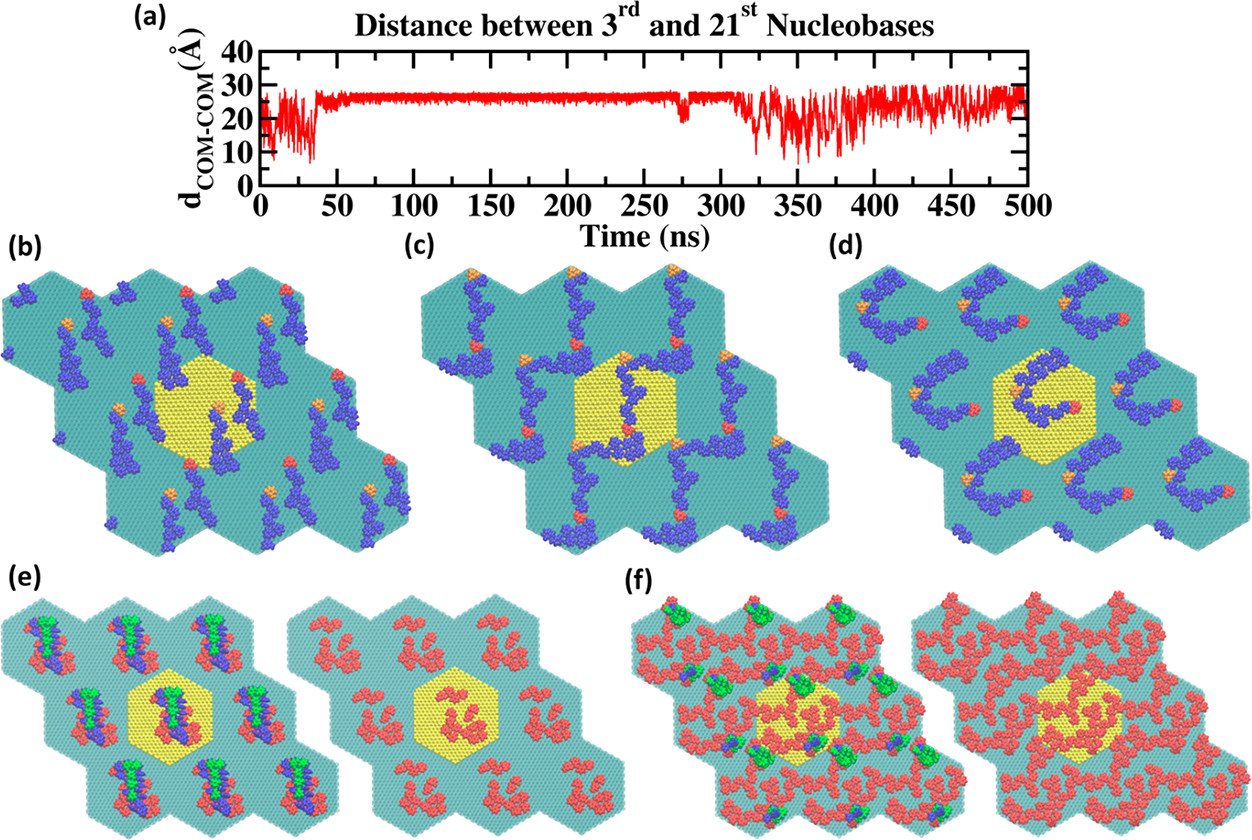
\includegraphics{Introduction/Figures/Figure8.png}
%     \caption[Representaive image depicting cytosine self-assemblies over graphene as a function of surface coverage]{(a) Time series of the center-of-mass to center-of-mass descriptor used to identify the nucleobase assemblies observed in 0.25 M simulations. Representative structures depicting the 2D network corresponding to (b) region-I, (c) region-II, and (d) region-III of the d\textsubscript{COM–COM} time series. Representative structures of nucleobase assemblies in (e) 0.50 M and (f) 0.75 M simulations. The simulation cell is indicated in yellow color and periodic images of the cell are colored green. (b–d) Nucleobases used in the center-of-mass metric are in red (3) and orange (21). All other nucleobases are colored blue. (e) and (f) Nucleobases are color-coded with respect to the distance from the graphene sheet. Nucleobases in regions (i) (d\textsubscript{Nuc–Graph} $<$ 4.5 $\angstrom$), (ii) (4.5 $\angstrom$ $<$ d\textsubscript{Nuc–Graph} $<$ 8.5 $\angstrom$), and (iii) (d\textsubscript{Nuc–Graph} $>$ 8.5 $\angstrom$) are presented in red, blue, and green, respectively. Reprinted (adapted) with permission from ref\supercite{h_capturing_2022}. Copyright 2023 American Chemical Society.}
% \end{figure}

% In a follow-up investigation, we demonstrated the transition of self-assembled monolayers from an ordered structure to a random arrangement depending on the concentration of the adsorbate (nucleobase) molecules.\supercite{h_capturing_2022} We investigated the self-assembly behaviour of cytosine nucleobases at three distinct concentrations covering the low (0.25M), medium (0.50M) and high (0.75M) concentration limits using classical Drude polarizable FF simulations. Our investigations showed that cytosine nucleobases at low concentrations can self-assemble into ordered 2D assemblies with significant lifetime, and the ordered self-assembly undergoes a steady transition towards a random arrangement of nucleobases with no perceived order with increasing concentration [Figure 1.11]. We also note that the self-assemblies we observed at 0.25M were structurally similar to the ones observed by Besenbacher and coworkers in cytosine molecules dispersed at a HOPG - 1-octanol interface via STM imaging.\supercite{xu_coadsorption_2006}

In the next section, we focus on few studies that have investigated the formation of mixed self-assemblies, where the structures are formed between two monomers of different chemical identity. It is imperative that such self-assemblies offer an important pathway towards realizing 2D networks of tunable properties, where the interactions can be tuned by intelligent choice of the interacting partners.

\subsection{Heterogeneous Systems}
\subsubsection{Experimental Studies}
\paragraph{Adenine-Thymine:}Besenbacher and coworkers investigated the formation of supramolecular self-assemblies at the interface of HOPG and 1-octanol using adenine and thymine nucleobases by employing STM imaging and DFT calculations.\supercite{mamdouh_supramolecular_2006} They observed the formation of a distinct AT supramolecular assembly which was constitutionally different from AA and TT pairings. From STM imaging, they observed two distinct regions: one row containing a cyclic substructure and another containing a 1D single chain, with the 1D chain interweaved between the rows containing cyclic substructures. They concluded from combinatorial DFT calculations that the observed AT heterostructure originates from interactions between two distinct subunits: two quartets of AT type and two sets of AA type [Figure 1.11(a-c)].

\begin{figure}
    \centering
    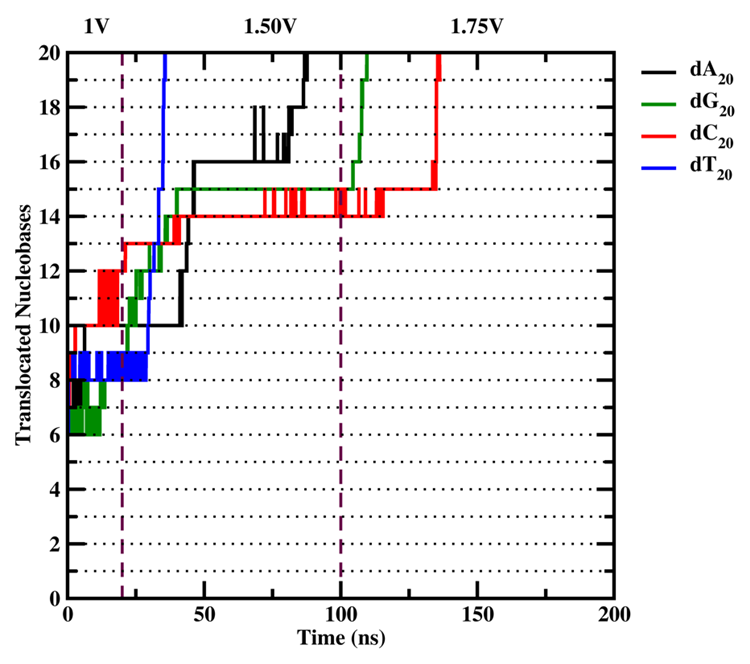
\includegraphics{Introduction/Figures/Figure10.png}
    \caption[STM images of A-T and G-U mixtures at the 1-octanol/graphite interface]{(a) STM image of A+T mixture at the 1-octanol/graphite interface. The tunneling parameters are I\textsubscript{tunn} = 1.2 nA and V\textsubscript{bias} = -447.4 mV. (b) Correlation-averaged zoom-in image of the area indicated in image (a) by a black square. (c) Calculated model suggesting that each cycle is composed of four molecules: 2A+2T, leading to reverse Hoogsteen A-T-A-T quartets adjacent to homochiral chains of A-A dimers. Cycles and A-A dimers are indicated with red rectangles and yellow ovals, respectively. The unit cell is indicated in black. Reprinted (adapted) with permission from ref \supercite{mamdouh_supramolecular_2006}. Copyright 2023 American Chemical Society. (d) High-resolution STM images of GU-base pairs at the 1-octanol/graphite interface. (e) zoom-in image of the yellow area indicated in A. Tunneling parameters are I\textsubscript{tunn} = 0.70 nA, V\textsubscript{bias} = 589.0 mV. (f) Molecular structure proposed by ab initio calculations. The GU-cyclic structures are indicated by yellow ovals, their size by blue arrows, and the unit cell lattice vectors are indicated. Green arrows indicate the hydrogen bonds between the GU-cyclic structures along unit cell vector a. Reprinted (adapted) with permission from ref \supercite{mamdouh_two-dimensional_2008}. Copyright 2023 American Chemical Society.}
    \label{fig:figure11}
\end{figure}

\paragraph{Guanine-Cytosine:} Besenbacher and coworkers investigated the formation of 2D self-assembled structures in a guanine-cytosine admixture at an HOPG-1-octanol interface using STM imaging and DFTB calculations.\supercite{xu_coadsorption_2006} They observed the formation of ordered self-assembly from the guanine-cytosine WC pairs formed from a 1D arrangement of interacting guanine and cytosine molecules. From STM images, they observed the formation of three distinct regions, where regions I and II corresponded to cytosine self-assemblies and region III corresponded to guanine-cytosine networks. DFTB calculations predicted two probable generating structures for the observed guanine-cytosine self-assembly, with two symmetric hydrogen bonds between -NH\textsubscript{2} and C2(O) extending the 1D chain. 

\paragraph{Guanine-Uracil:} Besenbacher and coworkers demonstrated the formation of a 2D self-assembled heterostructures from the interaction of guanine and uracil nucleobases at the interface of a HOPG surface and 1-octanol using STM imaging and DFT calculations.\supercite{mamdouh_two-dimensional_2008} They observed that the heterostructure formed from GU pairing substantially differed from the structures generated via the homogeneous pairing of nucleobases (GG and UU). They employed a systematic combinatorial DFT investigation to identify the unit cell corresponding to the observed GU heterostructure. They observed that only one among the multiple generated unit cells explained the obtained STM data [Figure 1.11(d-f)].

\subsubsection{Computational Studies}
\paragraph{ab-initio studies:} Cort\'{e}s-Arriagada investigated the adsorption of nucleobases and base pairs on graphene uisng PBE functional and obtained the following binding energies -14.53,  -18.68, -14.53, -14.07 and -12.45 kcal/mol for adenine, guanine, cytosine, thymine and uracil, respectively.\supercite{cortes-arriagada_phosphorene_2018} They also investigated the interaction of G-C, A-T and A-U pairs with graphene and the interaction energies of -28.13, -27.44 and -25.83 kcal/mol. The authors noted that the base pairs underwent preferential adsorption in the armchair direction of the surface.

In a follow-up study\supercite{cortes-arriagada_intermolecular_2021}, the same author investigated the binding of nucleobases and base pairs with the graphene surface using ab-inito calculations at the same level of theory as the previous study\supercite{cortes-arriagada_phosphorene_2018}. In this study, the author also investigated the effect of solvation on the binding energies using the conductor-like polarizable continuum model (CPCM) available in ORCA. The binding energies obtained for gas-phase (solvated) system were -12.91 (-10.61), -16.60 (-10.84), -12.91 (-7.61), -12.68 (-10.38), -11.07 (-8.54) kcal/mol for adenine, guanine, cytosine, thymine and uracil, respectively. They observed that the binding energies for single nucleobases interacting with a graphene surface in gas-phase followed the relative ordering of G $>$ A $>$  C $>$ T $>$ U, while the ordering became  G $>$ A $>$  T $>$ U $>$ C upon solvation. For base-pairs, the binding energies obtained were -25.14 (-20.30), -24.91 (-20.99) and -22.60 (-18.69) kcal/mol for C-G, A-T and A-U base pairs, with relative ordering being C-G $>$ A-T $>$ A-U in gas-phase and  A-T $>$ C-G $>$ A-U upon solvation. They observed that solvation drastically reduced the interaction energies between the nucleobases and the graphene surface, due to water screening the interactions between the nucleobases and the graphene surface. 

\paragraph{Molecular Dynamics Simulations:} Řezáč and coworkers investigated the differences between the propensity for hydrogen bonding interactions and $\pi$-stacking interactions between the nucleobases in three different conditions: vacuum, solvated and in the presence of solid support (graphene) using enhanced sampling MD simulations.\supercite{spiwok_free-energy_2011} They demonstrated a notable difference in the stabilizing interactions between the nucleobases in these conditions, with vacuum simulations predominantly stabilized via hydrogen-bonding interactions, while solvated systems preferred $\pi$-stacking interactions. In contrast, nucleobases preferentially interacted via hydrogen bonding interactions in the presence of solid support like graphene [Figure 1.12]. The authors reasoned that the strong preference of the nucleobases to first interact with the graphene surface via $\pi$-stacking interactions drives the later formation of the hydrogen bonding interactions between the nucleobases. This observation agrees with the calculated interaction energies: 19.1 - 26.3 kcal/mol for graphene-nucleobase $\pi$-stacking interactions, while A-T and G-C hydrogen bonds are at -13.1 and -17.5 kcal/mol, respectively.

\begin{figure}
    \centering
    \includegraphics[width=\textwidth]{Introduction/Figures/Figure6_md.png}
    \caption[Free-energy surfaces of the association of mA–mT and mG–mC pairs on graphene. Representative structures for minima are also presented]{Free-energy surfaces of the association of mA–mT and mG–mC pairs on graphene, calculated as the negative of the metadynamics bias potential. Representative structures for Minima A–N are also presented. The axes are the collective variables describing base stacking and Watson–Crick pair formation. Snapshots of the metadynamics simulations corresponding to minima A–N. The structures of the purines are superimposed within a group. These minima are Watson–Crick pairs (B,K), stacked pairs (F,N), dissociated bases (A,G), and other hydrogen-bonded arrangements (others). Reprinted (adapted) with permission from ref \supercite{spiwok_free-energy_2011}. Copyright 2023 American Chemical Society.}
    \label{fig:figure12}
\end{figure}

Mittal and coworkers demonstrated the influence of hydrogen bonding interactions in stabilizing the DNA base pairs adsorbed over a graphite surface.\supercite{shankar_dna_2012} They employed all-atom MD simulations to investigate the binding free energies of all possible combinations of nucleoside dimer pairs interacting with the graphene surface. They observed that the formation of non-Watson-Crick-type hydrogen bonding interactions between the adsorbed nucleosides accords extra stabilization to them. They obtained a relative ordering (energies in kcal/mol) of guanine-cytosine (-3.49) $>$ adenine-guanine (-3.08) $>$ adenine-thymine (-2.82) $>$ adenine-adenine (-2.18) $>$ cytosine-thymine (-2.09) $>$ guanine-guanine (-1.92) $>$ cytosine-cytosine (-1.77) $>$ adenine-cytosine (-1.40) $>$ thymine-thymine (-1.36) $>$ guanine-thymine (-0.79) for the interacting nucleosides. The authors also note that the $\pi$-stacking interactions between the nucleobases and the graphene surface primarily drive the dynamics. This observation agrees with the results obtained by Řezáč et al.,\supercite{spiwok_free-energy_2011} who investigated the interactions between nucleobases adsorbed over a graphite surface.

Thus, we note that hydrogen bonding interactions and vdW interactions are the two major factors in the formation and stabilization of 2D self-assembled monolayer structures. An accurate description of such interactions are required to understand the mechanisms behind the formation of such structures. ab-initio calculations capture the energetics of such interactions but fail to provide insights into the time evolution of such interactions. Molecular Dynamics simulations provide insights into the time evolution of such interactions. However, non-polarizable additive simulations do not capture the formation of self-assembled structures. 

Having discussed the self-assembly of nucleobases over a graphene (graphite) surface, we now focus on the experimental and theoretical studies on the applicability of graphene nanodevices for rapid and accurate sequencing of DNA. We first describe pioneering experimental studies that demonstrated the applicability of graphene membranes as suitable candidates for DNA sequencing before discussing the potential associated issues. We then discuss the computational studies based on MD simulations to provide an atomistic insight into the translocation dynamics of the DNA strands as they move through the nanopore.

\section{Graphene Nanodevices for DNA Sequencing}
Nanopores have attracted significant attention from the scientific community as a suitable tool towards rapid and accurate detection of a wide variety of molecules.\supercite{cherf_automated_2012, manrao_reading_2012, sutherland_structure_2004, chuah_nanopore_2019, liu_two-way_2013, cai_solid-state_2021, goyal_use_2015, baaken_high-resolution_2015} The basic working principle behind nanopore sequencing is that the flow of ionic current through the nanopore is sensitive towards the translocation of the molecule through the nanopore, and the measurement of this ionic current could serve as a marker towards the identification of the specific nucleobase occupying the nanopore at that instant. One of the first demonstrations of the applicability of nanopores in the detection of ssDNA and RNA molecules came from a study by Kasianowicz and coworkers, who demonstrated that the ionic current in the system was sensitive towards the translocation of ssDNA (RNA) molecules through the $\alpha$-hemolysin pore, providing a marker to identify the translocation of molecules through the nanopore.\supercite{kasianowicz_characterization_1996} Studies based on nanopores in \textit{Mycobacterium smegmatis} porin A (MspA)\supercite{faller_structure_2004} have demonstrated that they are a suitable alternative to $\alpha$-hemolysin nanopores due to a single sensing region with a diameter of $\approx$ 1.2 nm and length of $\approx$ 0.5 nm, in contrast to the three sensing regions in $\alpha$-hemolysin with a length of $\approx$ 5 nm and a diameter of $\approx$ 1.4 nm at the smallest point\supercite{stoddart_single-nucleotide_2009,stoddart_multiple_2010}. Even though biological nanopores have been tremendously successful in sequencing applications\supercite{stoddart_single-nucleotide_2009,stoddart_multiple_2010,bates_dynamics_2003,vercoutere_discrimination_2003,nakane_nanosensor_2004,stoddart_nucleobase_2010,ayub_individual_2012,di_muccio_insights_2019,wang_retarded_2020}, they suffer from a few significant drawbacks: (i) they have high sensitivity towards temperature and pH, and (ii) they cannot be reused immediately after being used once; both of which severely restricts its operational scope.\supercite{haque_solid-state_2013}

Solid-state nanopores, such as the ones constructed in graphene and SiN\textsubscript{x}, offer a viable alternative towards biological nanopores. They have high chemical and thermal stability and can be reused multiple times, negating the drawbacks associated with biological nanopores. However, the initial excitement associated with the application of solid-state nanopores in SiN\textsubscript{x} and SiO\textsubscript{2} soon died out when it was realized that it is impossible to achieve single-molecule resolution due to the large sensing regions ($>$10 nm), leading to multiple nucleobases occupying the nanopore at the same time\supercite{li_dna_2003,storm_translocation_2005}. It was soon identified that a single-molecule resolution could be achieved by reducing the sensing area, and 2D materials such as graphene\supercite{garaj_graphene_2010,schneider_dna_2010,wells_assessing_2012,merchant_dna_2010}, \textit{h}-BN and MoS\textsubscript{2}\supercite{liu_spontaneous_2020,qiu_detection_2017,zou_spontaneous_2020,luan_spontaneous_2018} began to be investigated as suitable membranes for sequencing applications. In particular, the inter-layer spacing between two graphene layers is 3.4 $\angstrom$, which is identical to the distance between two adjacent nucleotides in a DNA strand, indicating the possibility that graphene could be a suitable membrane for DNA sequencing applications.

In this context, we now discuss pioneering experiments and simulations that demonstrated the applicability of graphene membranes for DNA sequencing applications. We divide the discussion into translocation of dsDNA and ssDNA since both these cases present different translocation behaviours.

\subsection{double-stranded DNA (dsDNA)}
\subsubsection{Experimental Studies}
\begin{figure}[!h]
    \centering
    \includegraphics[width=\textwidth]{Introduction/Figures/figure_dsDNA_expt.png}
    \caption[Results from dsDNA - graphene nanopore experiments]{(a) Representaive image depicting graphene nanopore device. Ionic current trace of DNA translocation events (b) Time trace of DNA translocation events indicating unfolded, partially folded, and fully folded entries. (c) Histogram of blocked currents for measured translocation events for the nanopore device at V\textsubscript{B}=100 mV in 1 M KCl solution. Scatter plot of event length vs event depth at V\textsubscript{B}=100 mV with regions of unfolded and folded events highlighted inside the circled areas. Panel (a) reprinted (adapted) with permission from ref \supercite{garaj_graphene_2010}. Copyright 2023 Nature Publishing Group. Copyright 2023 American Chemical Society. Panel(b) reprinted (adapted) with permission from ref \supercite{schneider_dna_2010}. Copyright 2023 American Chemical Society. Panel(c) reprinted (adapted) with permission from ref \supercite{merchant_dna_2010}. Copyright 2023 American Chemical Society.}
    \label{fig:figure13}
\end{figure}

In 2010, Golovchenko and coworkers were one of the first groups to independently demonstrate that graphene membranes could be suitable for DNA sequencing.\supercite{garaj_graphene_2010} They employed an identical setup as the two other groups, with the graphene membrane placed above a SiN block and a 5-25 nm nanopore drilled into the graphene membrane by electron-beam drilling [Figure 1.13(a)]. They measured the ionic current across the graphene membrane and demonstrated the appearance of a larger blockage current associated with the translocation of DNA through the graphene nanopore.

In 2010, Dekker and coworkers independently demonstrated the applicability of graphene membranes as functional materials for DNA sequencing.\supercite{schneider_dna_2010} They demonstrated the successful translocation of a double-stranded DNA (dsDNA) through nanopores of various diameters ranging from 5-25 nm. They observed signals corresponding to three distinct modes of translocation: non-folded, partially folded and fully folded [Figure 1.13(b)]. They obtained translocation speeds of approximately 17,000 bp ms\textsuperscript{-1}, considerably slower than those achievable in SiN pores at 40,000 bp ms\textsuperscript{-1}.

Drndi\'{c} and coworkers also demonstrated one of the first experimental realizations of employing a graphene nanopore as a functional material for DNA sequencing in 2010 [Figure 1.13(c)]. They investigated a variety of devices with varied nanopore diameters (5-10 nm) and thicknesses (1-5 nm).\supercite{merchant_dna_2010} They were able to achieve higher blockage currents in comparison to traditional solid-state nanopores. They obtained an average velocity between 200,000 and 330,000 bp ms\textsuperscript{-1}, which was comparable to the velocities obtained from other solid-state nanopores. It was observed that bare graphene membranes were unsuitable for DNA sequencing applications due to the significant ion current noise and low yields, with only 10\% of the fabricated 50 devices having detectable DNA translocation. However, it was also noted that the deposition of a 5 nm thick layer of titanium dioxide resulted in a significant reduction in the noise in the observed ionic current and increased stability of the bare graphene pores.

Branton and coworkers investigated the efficacy of nanopores constructed in single-layer graphene membranes in detecting DNA bases with single-molecule resolution\supercite{garaj_molecule-hugging_2013}. The authors reported the fabrication and characterization of nanopores of varying diameters in single-layer graphene membranes and the effect of pore diameter on the detection resolution. They observed that graphene nanopores with a pore diameter comparable to the diameter of the dsDNA have high sensitivity and subnanometer resolution. The authors also employed numerical modelling to explain the experimental results and to estimate the parameters of the nanopore and the DNA molecule, such as the ion-conducting diameter, the length, and the blocking diameter. They observed that the translocation of dsDNA through the nanopore differed according to the diameter of the nanopore employed, with larger nanopores allowing for the translocation of dsDNA either in a long unfolded state or a folded state, while smaller nanopores allowed only for unfolded states. The authors also showed that dsDNA would denature at high pH, and the translocation of the ssDNA produced subsequently was considerably slower due to the interactions with the graphene surface. 

Radenovic and coworkers investigated a nanopore drilled onto a graphene nanoribbon as a suitable device for DNA detection\supercite{traversi_detecting_2013}. They investigated two markers to identify the translocation of DNA molecules through the nanopore: (i) the ionic current in the system and (ii) the transverse current flowing across the graphene nanoribbon. The authors observed that they could reliably identify the translocation events by correlating the dips (spikes) in the ionic current (transverse current) and found a significant correlation between these two events. The authors also reasoned that the random uncorrelated spikes in the ionic and transverse currents could be explained by considering that the DNA molecules can approach the nanopore without undergoing translocation, and can result in a weak blocking of the ionic current in the system. In contrast, the spikes in transverse current might have their origins in the electronic interactions between the graphene nanoribbon and charged molecules in solution.

An important issue concerning employing graphene nanopores for the reliable and efficient sequencing of dsDNA(ssDNA) is the significant 1/f noise in the experimental readouts of ionic currents. In one such study, Dekker and coworkers investigated the various factors that can lead to the observed noise in the measurements and noted that the noise was substantially reduced upon increasing the thickness of the nanopore, pointing to the mechanical fluctuations in the graphene sheet as a possible origin for the observed noise\supercite{heerema_1f_2015}. In this study, the authors investigated the following factors to determine its effect on the 1/f noise: (a) Pore diameter, (b) Salt concentration, (c) Effect of substituent groups and (d) Membrane thickness. A linear relationship was found between the pore size (diameter) and the observed noise, and a larger pore leads to a smaller noise. A very minimal correlation was observed between the salt concentration and the observed noise. It was found that the pore size and salt concentration could not explain the high 1/f noise observed in the experiments. The effect of substituent groups and the subsequent modification in the number of charge carriers on the observed noise were investigated by introducing carboxyl groups at the pore edges. No significant correlations were observed between the 1/f noise and the modulation of charge carriers, indicating that substituent groups are also not responsible for the observed noise. A significant correlation was observed between the membrane thickness (number of graphene layers) and the 1/f noise. It was found that the noise underwent significant reduction upon increasing the number of graphene layers, with a 1.5 times reduction in the noise levels when the layer thickness was increased from 1 to 20 graphene layers. The authors reasoned that the mechanical behaviour of the graphene layers was the reason for the significant 1/f noise observed in the graphene membranes. Few-layer graphene sheets can have significant oscillations in the sheets, inducing low-frequency noise in the measured ionic current readouts by modifying the ionic flux across the membrane.

In an unrelated study, Kim and coworkers also investigated the origins of 1/f noise in graphene-based devices, and they investigated devices consisting of few-layer graphene on top of quartz and silicon nitride substrates\supercite{kumar_noise_2013}. Initially, they investigated the effect of substrate on the 1/f noise in graphene. They found that the quartz-based device displayed a lower noise than the silicon nitride based device. Next, they investigated the effect of the number of layers on the noise. They observed that the few-layer graphene on a quartz device had significantly lower noise than single-layer graphene on a quartz device. They demonstrated that an FLG device would enhance the ionic current and spatial resolution and improve the signal-to-noise ratio.

\subsubsection{Molecular Dynamics Studies}
Schulten and coworkers employed all-atom MD simulations to investigate the translocation of dsDNA through a graphene nanopore, to understand its efficacy as a sequencing tool.\supercite{sathe_computational_2011} They investigated a variety of descriptors, namely - pore size, the strength of an external electric field, DNA conformation and pore charge, and its effect on the calculated ionic current. They observed that a larger pore diameter would be beneficial in capturing the DNA strand in comparison to a smaller pore, as the capture of the diffusion of the DNA strand towards the pore mouth precedes the capture of the DNA by the pore, with the non-linear potential drop across larger pores facilitating this movement. While investigating the effect of pore charge on the translocation of DNA strands, they observed that positively charged pores resulted in faster translocations than negatively charged pores due to the electrostatic repulsion between the pores and the negatively charged DNA. They also demonstrated that ionic current measurement could discern between A-T and G-C pairs. Applying a suitable external bias in MD simulations is the key to breaking A-T hydrogen bonds selectively, resulting in different ionic current signatures compared to G-C pairs [Figure 1.14(a)].

\begin{figure}
    \centering
    \includegraphics[width=\textwidth]{Introduction/Figures/figure_dsDNA_sim.png}
    \caption[Results from dsDNA - graphene nanopore all-atom MD simulations]{(a) Ionic current traces, CoM positions and averaged potential maps for dsDNA through graphene nanopores at various applied external biases. Ionic curent for poly-(AT)\textsubscript{20} and poly-(GC)\textsubscript{20} duplexes at different applied external biases. (b) Representative snapshots depicting the progress of dsDNA translocation through a graphene-\textit{h}-BN heterostructure nanopore. (c) Scatter diagram of CoM positions abd overlapped conformations of dsDNA at different external biases.Panel (a) reprinted (adapted) with permission from ref \supercite{sathe_computational_2011}. Copyright 2023 American Chemical Society. Panel (b) reprinted (adapted) with permission from ref \supercite{balasubramanian_dna_2021}. Copyright 2023 American Chemical Society. Panel (c) reprinted (adapted) with permission from ref \supercite{qiu_electrically_2016}. Copyright 2023 American Chemical Society.}
    \label{fig:figure14}
\end{figure}

Balasubramanian and coworkers investigated the translocation dynamics of a dsDNA through a nanopore constructed in graphene-\textit{h}-BN heterostructure using MD simulations\supercite{balasubramanian_dna_2021}. They observed that on average poly-(AT) strands required more time to complete translocations in comparison to poly-(GC) strands, with the average time being 13-24 ns for poly-(GC) strands and 28-46 ns for poly-(AT) strands. The authors reasoned that the longer translocation time of the poly(AT) sequence is based on the fact that the DNA-substrate interaction with graphene significantly distorts the double helix structure in poly-(AT) strand, leading to the dsDNA behaving as two uncorrelated ssDNA strands, and resulting in a decrease in the transverse mobility of the poly(AT) sequence (across the nanopore) consequently leading to a longer translocation time. In constrast, the double-helix structure of the poly-(GC) strand remains almost intact, leading to shorter translocation times, in general [Figure 1.14(b)].

Leburton and coworkers employed all-atom MD simulations to investigate the effect of applied external biases and the pore geometry on the conformational dynamics of the dsDNA residing within the nanopore\supercite{qiu_electrically_2016}. To this end, they first investigated the effect of multiple applied external biases on the conformational dynamics of dsDNA. They observed that a positive applied external bias reduced the fluctuations in the dsDNA due to the increased electrostatic interactions between the negatively charged dsDNA backbone and the positively charged pore walls. In contrast, they observed that a negative applied external bias resulted in more significant fluctuations in dsDNA due to the strong repulsion between the negatively charged DNA backbone and the negatively charged pore walls [Figure 1.14(c)]. To investigate the effect of pore geometry on the conformational dynamics of the dsDNA, the authors investigated the dynamics of dsDNA in a tear-drop-shaped nanopore at three voltages: -0.5 V, 0 V and 0.5 V. The authors demonstrated that at 0.5 V, the DNA strand moved towards the sharp end of the nanopore, where a slower decay of the applied external bias is expected. In contrast, the strand was located at the broader end of the nanopore during 0 V and -0.5 V simulations, indicating that fluctuations within the DNA strand can be controlled via careful choices of pore geometries and applied external biases.

Wu and coworkers investigated the effect of nanopore thickness on the translocation dynamics of a dsDNA through a graphene nanopore with varying radii and applied external biases\supercite{lv_impact_2013}. They investigated a range of nanopore thickness (1-3 layers) and pore radii (2, 2,4 and 3 nm) at applied external biases of 1-4 V, and observed that the layer thickness was inversely correlated with the speed of the translocations, with thicker nanopores slowing down the translocation of the dsDNA through the nanopore. They also observed that higher applied external biases could effect translocations even in thicker nanopores, which would otherwise be devoid of any observable translocations.

Wu and coworkers employed all-atom MD simulations to investigate the correlation between the calculated ionic current and the spatial orientations of the dsDNA strand while moving through the nanopore\supercite{lv_spatial_2014}. The authors investigated multiple systems with two different applied external biases to evaluate the effect of spatial orientations of dsDNA on the calculated ionic current. They observed that the local conformations adopted by the DNA strand significantly affected the ionic current. From further analysis of the ionic current trace and the dynamics of the dsDNA strand, they also concluded that the interactions between the DNA strand and the graphene sheet can influence the ionic current. Further, they also observed that the ionic current depends on the location of the DNA strand with respect to the nanopore.

\subsection{single-stranded DNA (ssDNA)}
\subsubsection{Experimental Studies}
\begin{figure}
    \centering
    \includegraphics[width=\textwidth]{Introduction/Figures/figure_ssDNA_expt.png}
    \caption[Results from ssDNA - graphene nanopore experiments]{(a) Ionic current trace obtained for pristine graphene nanopore incubated with ssDNA. Timesteps where large 1V pulses (red dots) were applied are also indicated. (b) STM image for the pristine graphene nanopore. (c) STM image for the same nanopore after the experiment, demonstrating pore clogging. Reprinted (adapted) with permission from ref \supercite{schneider_tailoring_2013}. Copyright 2023 Nature Publishing Group.}
    \label{fig:figure15}
\end{figure}

Hydrophobic interactions between the ssDNA strand and the graphene surface are a limiting factor in the translocation of the ssDNA strand through the graphene nanopore, with significant pore clogging observed when pristine graphene membranes are employed [Figure 1.15]. Schnider and coworkers demonstrated that a SAM with a long hydrophilic alkyl chain could be a suitable anti-fouling agent to tune the interactions between the ssDNA strand and the graphene surface.\supercite{schneider_tailoring_2013} They constructed the SAM from two molecular cores - a hydrophobic aminopyrene and a tetraethyleneglycol monomethyl ether N-hydroxysuccinimide ester, where the aminopyrene molecules interact with the graphene surface and the long alkyl chain protruding out into the solution, rendering the graphene surface hydrophilic. From AFM studies, they observed that the ssDNA did not adsorb onto the SAM-coated graphene surface, even at high loading limits of 10 ng $\mu$l\textsuperscript{-1}. They also demonstrated unhindered translocations of ssDNA through the graphene nanopore, in contrast to the pristine graphene nanopore, where significant pore clogging necessitated the application of high voltage (1V) to effect translocations.

While hydrophobic interactions between the graphene surface and DNA leads to pore clogging, slowing down the transport of DNA across the graphene membrane is also essential to achieve sufficient temporal resolution in ionic current measurements. To this end, Aksimenteiv and coworkers constructed two devices - a graphene-alumina-graphene membrane and an alumina-graphene-alumina membrane to investigate the translocation dynamics.\supercite{banerjee_slowing_2015} They investigated the transport of dsDNA and ssDNA through these membranes. For ssDNA translocation, they observed a significant reduction in the translocation velocity ($\approx$ 180 nt ms\textsuperscript{-1}) compared to a native alumina membrane ($\approx$ 550 nt ms\textsuperscript{-1}) due to the increased interaction between the ssDNA and graphene surface. The hydrophobic interactions between the nucleobases and the graphene surface are absent for dsDNA for two reasons: (a) because of  Watson-Crick hydrogen bonding interactions and (b) the presence of a negatively charged phosphate backbone. Thus, they underwent translocations significantly faster compared to ssDNA, with a translocation velocity of 2500 bp ms\textsuperscript{-1}, which is approximately an order of magnitude faster than the translocation velocity for an ssDNA through a graphene-alumina-graphene membrane. The difference in translocation speeds for ssDNA and dsDNA demonstrated that the hydrophobic interactions between the graphene surface and the ssDNA could result in longer dwell times and significantly better temporal resolution in ionic current measurements.

\subsubsection{Molecular Dynamics Studies}
\begin{figure}
    \centering
    \includegraphics[width=\textwidth]{Introduction/Figures/figure_ssDNA_sim}
    \caption[Results from ssDNA - graphene nanopore all-atom MD simulations]{(a) Representative figures depicting the system setup and progress of translocations of ssDNA through nanopores of varying thicknesses. (b) Hydrogen bonds between poly(dA) and poly(dT) with DNA origami. (c) Representative snapshots of translocated nucleotides of ssDNA in circular, square and triangular graphene–MoS\textsubscript{2} heterostructure nanopores.  (d) Representaive images depicting the three pulling directions investigated and the motion of ssDNA along the defect channels under an applied external force. Panel (a) reprinted (adapted) from ref \supercite{wells_assessing_2012}. Copyright 2023 American Chemical Society. Panel(b) reprinted (adapted) with permission from ref \supercite{barati_farimani_dna_2017}. Copyright 2023 American Chemical Society. Panel (c) reprinted (adapted) with permission from ref \supercite{zou_spontaneous_2020}. Copyright 2023 American Chemical Society. Panel (d) reprinted (adapted) with permission from ref.\supercite{shankla_step-defect_2019}. Copyright 2023 Nature Publishing Group.}
    \label{fig:figure16}
\end{figure}

Using all-atom MD simulations, Aksimenteiv and colleagues demonstrated that few-layer graphene membranes can act as suitable tools for rapid and accurate sequencing of ssDNA.\supercite{wells_assessing_2012} They investigated the translocation dynamics of four ssDNA homopolymers (adenine, guanine, cytosine and thymine) through multiple pore geometries and membranes of various thicknesses using non-polarizable additive FF simulations [Figure 1.16(a)]. They demonstrated that the interactions between the graphene surface and the ssDNA strand could significantly slow the transport of ssDNA across the graphene membrane. They noted that the transport of ssDNA across the graphene membrane occurs in single nucleotide steps. However, they also noted that the transport mechanism does not proceed in one direction leading to multiple entries and exits being registered for a single nucleotide, eventually leading to an erroneous readout of the ssDNA sequence.

Aluru and coworkers employed all-atom MD simulations to evaluate the translocation dynamics of an ssDNA through a DNA origami-decorated graphene nanopore.\supercite{barati_farimani_dna_2017} They employed a modified DNA strand with eight adenine nucleotides removed from the template strand, leaving eight free thymine nucleotides of the complementary strand as a decorator over the nanopore. They observed that at a particular voltage, the transport of the ssDNA across the hybrid nanopore depends on the interactions between the ssDNA and the DNA origami, with the dwell time of $\sim$ 3 ns for polydA, due to its interaction with the complementary T nucleotides in the DNA origami [Figure 1.16(b)]. Even though DNA origami only had free T nucleotides, the formation of hydrogen bonds between the polydC strand and the G-C base pairs in the DNA origami led to a significant dwell time for polydC strands. From ionic current measurements, they demonstrated that ionic current measurements could reliably identify A and G bases, while T and C bases have similar ionic currents. The authors opined that a statistical analysis of ionic current and dwell times could reliably identify the four bases.

Zhou and colleagues investigated the effect of various pore geometries in a graphene-MoS\textsubscript{2} heterostructure on the spontaneous transport of ssDNA across the membrane, using MD simulations\supercite{zou_spontaneous_2020}. They observed significantly slower translocations in triangular nanopores, while the translocations were observed to be the fastest in circular nanopores [Figure 1.16(c)]. Their observations of the spontaneous transport of ssDNA across the heterostructure were rationalised using the electrostatic interactions between the positively charged Mo ions and the negatively charged phosphate (PO\textsubscript{4}\textsuperscript{-}) groups in the ssDNA. This observation of spontaneous transport of ssDNA under the influence of chemical potential, and without an explicit applied external bias is in line with the previous observations by Zhou and coworkers, where a similar transport was observed from MD simulations\supercite{luan_spontaneous_2018}.

Shankla and Aksimenteiv investigated the motion of an ssDNA along a step-defect using all-atom MD simulations\supercite{shankla_step-defect_2019}. Using constant velocity-steered MD (SMD) simulations, the authors demonstrated a sharp increase in the force acting on the ssDNA molecules at a defect junction, which quickly drops to zero once the molecule has crossed the junction. They also noted a directional dependence on the force, with a higher force ($\approx$ 2-2.5 times) required to pull the ssDNA up a defect junction than to move it down a defect junction. The authors reasoned that the origin of this difference could be attributed to the hydration of the nucleotide, with the nucleotide losing the hydration as it moves up the defect junction and then getting rehydrated once it moves past the junction. In contrast, while the nucleotide moves down the defect junction, it first gains hydration, which is then lost as it moves across the junction, and finally regains the hydration as it moves past the defect junction. The authors also demonstrated that a step-guided pattern that transport ssDNA either towards or away from a nanopore [Figure 1.17(d)]. 

Shankla and Aksimenteiv employed all-atom MD simulations to also study the translocation dynamics of an ssDNA through a charged graphene nanopore\supercite{shankla_conformational_2014}. The authors used a poly-dT\textsubscript{20} strand to model an ssDNA and investigated the dynamics of the ssDNA through three nanopores, where the graphene sheets had a surface charge density between -2 and 2e/nm\textsuperscript{2} in steps of 0.5. They observed that the charge of the graphene sheet has a significant effect on the dynamics of the ssDNA, with the interactions between the ssDNA and the graphene surface being drastically different between -2e/nm\textsuperscript{2} and 2e/nm\textsuperscript{2} simulations. For a charge-neutral system (0e/nm\textsuperscript{2}), they observed that the strand has significant interactions with the graphene sheet via stacking interactions between the nucleobases and the surface. At the same time, the negatively charged phosphate groups did not interact with the surface. However, upon increasing the charge to +2e/nm\textsuperscript{2}, they observed that the nucleobases' orientation had changed to 47$\degree$ from 0$\degree$, indicating that the negatively charged phosphate groups had started interacting with the positively charged graphene surface. On a similar footing, changing the surface charge density to -2e/nm\textsuperscript{2} has the opposite effect, where the ssDNA would be repelled away from the graphene surface. The authors observed that these interactions are reversible, meaning it is possible to convert from one state to another by changing the surface charge density on the graphene surface. For other homopolymers considered in the study (dA\textsubscript{20}, dG\textsubscript{20}, dC\textsubscript{20} and a methylated version of dC\textsubscript{20}), very similar dynamics were observed where some or all nucleobases were observed to be repelled away from the surface at a surface charge density of -2e/nm\textsuperscript{2}. However, they observed different dynamics at the other end of the surface charge density (2e/nm\textsuperscript{2}), where some combination of orientations (flat, tilted and unbound) were observed for the four homopolymer strands. To comment on the effect of surface charge density on the translocation of ssDNA through the nanopore, the authors investigated the translocation of ssDNA through the same nanopores at an applied external bias of 500 mV. They observed that the translocation velocity of the dT\textsubscript{20} strand depended on the surface charge density, with the translocation velocity varying in a correlated manner with the surface charge density. As a proof-of-concept, the authors also demonstrated a stop-and-go type of dynamics for the ssDNA by changing the surface charge densities and the applied external bias, where they demonstrated that under a constant applied external bias, changing the surface charge density would halt the translocation of the ssDNA through the nanopore.  

Smolyanitsky and coworkers employed all-atom MD simulations to investigate the applicability of a cytosine-decorated graphene nanopore as a functional material for DNA sequencing.\supercite{paulechka_nucleobase-functionalized_2016} They studied the efficacy of the functionalized nanopore in detecting guanine nucleobases present in the ssDNA strand by using the ripples generated in the graphene nanoribbon (GNR) during the translocation of ssDNA. They demonstrated that a cytosine-functionalized nanopore could reliably identify guanine-rich segments in the translocating ssDNA.

Schulten and coworkers investigated the translocation dynamics of poly-dA\textsubscript{14} through a nanopore constructed in a graphene nanoribbon using steered molecular dynamics (SMD) simulations\supercite{qiu_intrinsic_2015}. They observed that the ssDNA would undergo quicker translocations if the 3'-end of the ssDNA is threaded through the nanopore, in contrast to the 5'-end where the translocations were more sluggish, giving rise to the step-wise translocations previously reported in the literature.  They reasoned that by reversing the pulling direction inorder to translocate the 3' end of the ssDNA through the nanopore, the DNA bases can form a bigger angle with the graphene surface normal and, can move quicker through the nanopore; while pulling in the original direction, with the 5'-end translocating first, the DNA bases would form a smaller angle with the graphene surface, increasing the probability of the nucleobases getting stuck in the nanopore, giving rise to stepwise translocations.

\section{Conclusions}
Here, we have summarised a few critical experimental and computational investigations demonstrating the applications of graphene as a solid-state support for 2D SAM formation and a solid-state membrane for rapid and accurate DNA sequencing. These research studies underline the importance of graphene and (or) graphene-like materials as solid-state support and functional materials for biological applications. The electronic structure of graphene can be tuned based on the electronic nature of the adsorbed molecules, opening up the possibility of using graphene as a functional material for sensing applications. However, we note that MD simulations based on classical additive FFs need further improvement in describing the formation of such self-assemblies\supercite{saikia_hierarchical_2017,saikia_dynamics_2018}. Few authors investigated the development of FFs specifically parameterized to describe such interactions, but they are generally not transferable between systems\supercite{manukyan_first_2015}. Previous studies based on ab-inito calculations have demonstrated that the strength of the non-covalent interactions between the nucleobases and the underlying graphene surface is proportional to the molecular polarizability of the nucleobases and the surface.\supercite{gowtham_physisorption_2007} However, additive non-polarizable FF simulations, based on fixed point charges are unable to describe molecular polarizability, leading to errenous simulation outcomes. This indicates that a polarizable description for all the components is a necessary requirement towards understanding the self-assembly of nucleobases and (or) other small molecules at the graphene interface.  

The outbreak of the severe acute respiratory syndrome coronavirus 2 (Sars-Cov-2) and the swift progress in the development of treatment protocols hightlights the need for a fast, reliable and afforable method for DNA sequencing. In this context, graphene nanopores have emerged as a suitable material for DNA sequencing. Multiple authors have investigated various methodologies for efficiently using graphene membranes as a DNA sequencing tool. We want to highlight the work by Aksimenteiv and coworkers, where they demonstrated that two channels of opposite chirality can transport ssDNA across the nanopore without pore clogging\supercite{shankla_step-defect_2019}. Those simulations were performed using additive FF, and further investigations using classical Drude FF might be required to further understand ssDNA's transport across the nanopore. We note that investigations about the specific effects of water and ions on the transport of DNA strands across the graphene membranes and their effects on the ionic and (or) transverse current measurements still need to be explored.

To this end, ionic conductivity and transport phenomena in nanopores, nanochannels is an active field of investigation with better representations required to capture the associated dynamics. Some recent developments to this end have been the use of non-equilibrium modelling to capture the concentration dependent dynamics.\supercite{nazari_transport_2020,karmakar_non-equilibrium_2023} Recent experimental studies have explored transverse detection of DNA strands using both graphene\supercite{heerema_probing_2018} and MoS\textsubscript{2} nanopores,\supercite{graf_transverse_2019} wherein nucleobase detection was observed in both the cases. Theoretically many groups have explored transverse current signatures of nucleobases trapped within a nanopore, however a limitation with this work is that these DFT bases calculations are performed using single layer nanopores.\supercite{prasongkit_transverse_2011,lagerqvist_fast_2006,prasongkit_theoretical_2015} A multilayer description must be adopted for a better description of nanopore interactions as evidenced by simulation studies.\supercite{wells_assessing_2012} We expect to see more investigations from both experimental and theoretical point of views aimed at investigating the transport of DNA molecules across nanopores.

\section{Thesis Objectives}
The overall objective of this thesis is to provide a generalized methodology to investigate the dynamics of small molecules in presence of a graphene surface. The specific objectives are:
\begin{itemize}
    \item To transfer and test the Drude polarizable FF parameters to describe a polarizable graphene sheet, and to investigate the dynamics of nucleobases in the presence of a polarizable graphene surface.
    \item To investigate the dynamics of mono and divalent ions in the presence of a graphene surface, to gain insights on the interaction patterns of the ions with the graphene surface.
    \item To investigate the dynamics of a ssDNA translocating through a pristine graphene nanopore, to gain insights into the experimentally observed pore clogging, and to gain insights into the various factors that affect the translocation dynamics. 
\end{itemize}

\section{Thesis Outline}
 Using all-atom MD simulations, in conjunction with Drude polarizable FF parameterization, we investigate the dynamics of nucleobases, ions and short ssDNA strands in presence of a polarizable graphene surface to gain a critical understanding of the interfacial dynamics. In this section, we provide a brief overview of the thesis. This thesis is divided into six chapters, with a brief description of each chapter provided here.

\begin{itemize}
    \item \textbf{Chapter 1} provides a survey of the literature pertaining to the applications of graphene and (or) graphite in the domains of nucleobase self-assemblies and as functional materials for DNA sequencing. 
    \item \textbf{Chapter 2} provides a brief overview of the simulation methods used in this thesis and also provides a summary of Adaptive Biasing Force simulations.
    \item \textbf{Chapter 3} reports the development of Drude polarizable FF paraneters for graphene, and the effect of molecular polarizability on the dynamics of nucleobases disperesed over a graphene surface.
    \item In \textbf{Chapter 4}, polarizable force field simulations elucidate the aggregation behaviour of nucleobases on a graphene surface as a function of solute concentration, providing valuable insights into their dynamics.
    \item In \textbf{Chapter 5}, polarizable force field simulations elucidate the dynamics of electrolyte solutions in close contact with a polarizable graphene surface. We also report an accurate reproduction of the ion-graphene interactions from polarizable simulations.  
    \item \textbf{Chapter 6} provides an atomistic description of the factors influencing the translocation dynamics of a single-stranded DNA (ssDNA) as it moves through a pristine graphene nanopore.
    \item \textbf{Chapter 7} provides an overall summary of the thesis and avenues for future work.
\end{itemize}

\section{List of Publications}
\begin{itemize}
    \item \textbf{H., Hemanth} and Mallajosyula*, S.S.; Polarization Influences the Evolution of Nucleobase - Graphene Interactions; {\textit{Nanoscale}, 2021, \textbf{13}, 4060 - 4072}
    \item \textbf{H., Hemanth}, Yadav, P. K. and Mallajosyula*, S.S.; Capturing Concentration Induced Aggregation of Nucleobases on Graphene Surface Through Polarizable Forcefield Simulations; {\textit{J. Phys. Chem. C}, 2022, \textbf{31}, 13122 - 13131}
    \item \textbf{H., Hemanth}, Mewada, R. and Mallajosyula*, S.S.; Capturing Charge and Size Effects of Ions at the Graphene - Electrolyte Interface Using Polarizable Force Field Simulations; {\textit{Nanoscale Adv.}, 2023, \textbf{5}, 796 - 804}
    \item \textbf{H., Hemanth} and Mallajosyula*, S.S.; Unveiling DNA Translocation in Pristine Graphene Nanopores: Understanding Pore Clogging via Polarizable Simulations; {\textit{ACS Appl. Mater. Interfaces}, 2023, \textbf{47}, 55095-55108} 
    \item \textbf{H., Hemanth} and Mallajosyula*, S.S.; Graphene: From Solid Support for Nucleobase Assisted Self-Assemblies to Functional Material for DNA Sequencing; {\textit{J. Phys. Chem. C}, 2024, \textbf{8}, 3091-3112} 
\end{itemize}

    \chapter[Theoretical Background and Methodology]{Theoretical Background and Methodology}
Molecular dynamics (MD) is a robust computational technique employed to explore the dynamic behaviour of atoms and molecules over time, offering microscopic insights into various physical and chemical phenomena. Its applications span diverse fields, including chemistry, physics, materials science, and biochemistry.

The origins of molecular dynamics can be traced back to the mid-20th century, with significant progress made in the following decades. Alder and Wainwright's pioneering work in the late 1950s laid the groundwork for numerically integrating classical equations of motion, enabling atomic-level simulations.\supercite{alder_studies_1959} Over time, computer hardware and algorithm advancements have propelled MD simulations to unprecedented accuracy and complexity.

The simulation entails solving Newton's equations of motion to predict the positions and velocities of atoms or molecules as they evolve. This computational approach yields valuable information on structural dynamics, thermodynamics, and kinetic properties of materials. The accuracy of MD simulations relies on the chosen force field, which mathematically models interactions between particles.

MD's significant contribution lies in unravelling the intricacies of biomolecular processes. Simulations of proteins, nucleic acids, and other macromolecules have proven invaluable for understanding protein folding, enzyme catalysis, and molecular recognition. These insights enhance our comprehension of molecular life and drive advancements in drug discovery and the design of targeted therapies.

Beyond biomolecules, MD plays a pivotal role in investigating the dynamics of solutions, enabling the study of liquids and gases in different environments. Its applications extend from understanding the properties of simple liquids to modelling complex solutions in chemical processes and environmental systems.

In summary, molecular dynamics offers a unique and powerful tool to investigate the dynamic nature of molecules and materials. Its applications across scientific domains drive advancements in our understanding of the natural world, facilitating the development of new technologies and solutions to complex problems.

In the context of this thesis, MD simulations were employed to investigate the dynamics of nucleobases, electrolyte solutions, and short ssDNA strands in the presence of a graphene surface. MD simulations involve solving Newton's equations of motion for numerous atoms at discrete time steps, generating a 3N-dimensional potential energy surface at each time slice, with the potential energy surface intricately tied to the atomic positions at each time step. The energy derivatives at each step are then utilized to propagate the coordinates and velocities to the subsequent step using one of the algorithms described below.

\section[Integration of Equations of Motion]{Integration of Equations of Motion}
\subsection[Integrators]{Integrators}
    \begin{itemize}
        \item \textbf{Verlet algorithm}\supercite{grubmuller_generalized_1991, gronbech-jensen_simple_2013}: The Verlet algorithm is a second-order integrator where the positions and velocities are propagated through time, starting from an initial set of coordinates and velocities. The Verlet algorithm is a numerically stable method. The algorithm is time reversible, meaning it is possible to run the integrator backwards to identify the dynamical trajectory's starting position due to the equations' lack of randomness. The basic algorithm does not require knowledge about the particle velocities to propagate the coordinates through time due to the algorithm's structure, which has a form described below.
        \begin{align*}
            x(1) &= x(0) + v(0)*\Delta t + \frac{1}{2}a(0)\Delta{t^2} \\
            x(t+1) &= 2x(t) - x(t-1) + a(t)\Delta{t^2}
        \end{align*}
        \item \textbf{Velocity-Verlet algorithm}\supercite{paterlini_constant_1998,marry_trotter_2007}: Velocity-verlet algorithm has explicit dependence on the velocities of the particles, and we use the velocities calculated at the midpoint of two consecutive timesteps in propagating the coordinates through time. The equations governing the Velocity-verlet algorithm have the form described below.
        \begin{align*}
            v(t + \frac{1}{2}\Delta{t}) &= v(t) + \frac{1}{2}a(t)\Delta{t} \\
            x(t+1) &= x(t) + v(t+ \frac{1}{2}\Delta{t})\Delta{t} \\
            a(t+1) &= F(t)/m \\
            v(t+1) &= v(t+\frac{1}{2}\Delta{t}) + \frac{1}{2}a(t+\Delta{t})\Delta{t}
        \end{align*}
        \item \textbf{Leapfrog algorithm}\supercite{toxvaerd_algorithms_1991,van_gunsteren_leap-frog_1988}: The Leapfrog algorithm is conceptually similar to the Velocity-verlet method in that positions and velocities leapfrog over each other in sequence. Similar to Verlet and Velocity-verlet algorithms, the leapfrog algorithm is also a second-order algorithm. 
    \end{itemize}

    \subsection{Constraints and Restraints}
    Traditionally, the bonds involving hydrogen atoms are constrained during an MD simulation, to allow for the ue of larger time steps in the integration of equations of motion. This is due to the fact that the time step of an MD simulation must be small enough to capture the fastest bond-stretching frequency, which would be for bonds involving hydrogen atoms.
    We use SETTLE\supercite{miyamoto_settle_1992} and SHAKE\supercite{ryckaert_numerical_1977} algorithms to constraint the necessary bonds in the MD simulations.

    When employing constraints, they are generally employed using lagrange multipliers, where the are $n$ holomonic constraints denoted as $\left\{ \sigma_1,\sigma_2,\cdots  \right\}$, we can express the lagrange multipliers as:
    \begin{align*}
        \sigma_k = \left\| r_i(t) - r_j(t)\right\|^2 - d_k^2
    \end{align*} 

    where $\sigma_k$ is the $k^{th}$ holonomic constraint, and $r_i$ and $r_j$ are the unconstrained positions of $i^{th}$ and $j^{th}$ atom involved in the $k^{th}$ holonomic constraint, and $d_{k}$ is the constrained bond length.

    In contrast, Restraints are generally applied to restrain one (or more) atoms in space. This is generally employed by attaching a spring on the restrained atom (atoms) with a user defined spring constant, such that the motion of the restrained atoms is arrested during the MD simulations. This is particulary useful when investigating surfaces, where you need to account for the surface vibrations, but also need to arrest the sliding motion of the surface.

    \subsection{Thermostats and Barostats}
    Thermostats and Barostats are typically employed to investigate a system in a particular ensemble (isobaric-isothermal or isochoric-isothermal), and a selection of thermostats and barostats which can be used for the same are described below: 

    \begin{itemize}
        \item \textbf{Velocity rescaling Thermostat}\supercite{woodcock_isothermal_1971}: This is the simplest form of themostat, where the atomic velocities at each step are rescaled by a factor $\lambda$ at a calculated temperature of $T(t)$, such that the rescaled velocities are at the desired temperature $T_0$.
        \begin{align*}
            \lambda = \sqrt{\frac{T(t)}{T_0}}
        \end{align*}

        \item \textbf{Berendsen Thermostat}\supercite{berendsen_molecular_1984}: In Berendsen Thermostat, the system is weakly coupled to an external heat bath, with an associated coupling constant $\tau$, such that the velocities at each step are rescaled by a parameter $\lambda$. Here, the temperatures are alloed to fluctuate, but the temperature $T(t)$ is dampened towards the target temperature $T_0$.
        \begin{align*}
            \lambda = \sqrt{\left[1 + \frac{dt}{\tau}\left(\frac{T_0}{T(t)}-1\right)\right]}
        \end{align*}

        \item \textbf{Andersen Thermostat}\supercite{andersen_molecular_1980}: In Andersen Thermostat, a predertmined number of atoms undergo collision with a stochastic bath particles, and are then assigned new velocities based on the Maxwell-Boltzmann distribution such that the canonical ensemble is correctly sampled. The time interval between two successive collisions is dependent on the collision frequency ($\nu$) and follows the Poisson distribution.

        \item \textbf{Langevin Thermostat}\supercite{schneider_molecular-dynamics_1978}: Langevin dynamics controls the system's temperature by introducing a Gaussian random error term, which readjusts the particles' velocities via collisions with virtual particles modelled via Gaussian random errors. However, the presence of this error term means that Langevin dynamics is not time-reversible, unlike other algorithms.
        \begin{align*}
            \ddot{r_i} = \frac{F_i - m_i\gamma v_i + F^{rand}_i}{m_i}
        \end{align*}
        Here, $\ddot{r}$ denotes the accelaration on the particle $i$, $\gamma$ denotes the friction coefficient, and $F^{rand}_i$ in a Gaussian random error term with a mean of zero and non-zero $\sigma$ calculated as:
        \begin{align*}
            \sigma_i = \sqrt{\frac{2m_i\gamma k_B T}{dt}}
        \end{align*}

        \item \textbf{Nos\'{e}-Hoover Thermostat}\supercite{nose_molecular_1984,hoover_canonical_1985}: In Nos\'{e}-Hoover Thermostat, the system is extended via the introduction of a virtual particle $\bar{s}$ with a mass $Q > 0$ and a velocity of $\dot{\bar{s}}$, with the magnitude of $Q$ determining the coupling between the heath bath and the system, and in turn determining the temperature fluctuations. The Hamiltonian for the extended system can then be written as:
        \begin{align*}
            \mathcal{H} = \frac{P_i^2}{2m_i} + U(r) + \frac{p_s^2}{2Q} + N_{free}k_BTln(s) 
        \end{align*}
        where $N_{free}$ is the available number of degrees of freedom.
    \end{itemize}

    Having discussed the available Thermostats, we now discuss the available Barostats.
    \begin{itemize}
        \item \textbf{Berendsen Barostat}\supercite{berendsen_molecular_1984}: In Berendsen Barostat, the coordinates and the cell vectors are rescaled at each time step, with the pressure $P(t)$ relaxing to a target pressure $P_0$ following the first order kinetic equation:
        \begin{align*}
            \frac{dP(t)}{dt} = \frac{P-P_0}{\tau_p}
        \end{align*}
        where $P(t)$ is the instantaneous pressure, $P_0$ is the target pressure and $\tau_p$ is the barostat relaxation time. 

        Here, the scaling matrix for the cell vectors is determined from the following equation:
        \begin{align*}
            \mu = 1 - \frac{dt\beta}{\tau_p}\left(P_0 - P(t)\right)
        \end{align*}
        where $\beta$ is the isothermal compressiblity of the system, and is usually set to a value of $4.6x10^{-10}$ Pa\textsuperscript{-1} which is the isothermal compressiblity of liquid water at 300 K and 1 atm pressure. The matrix $\mu$ will be diagonal with the elements $\mu_{xx} = \mu_{yy} = \mu_{zz}$ if the scaling is isotropic.

        \item \textbf{Nos\'{e}-Hoover Langevin Barostat}\supercite{feller_constant_1995,martyna_constant_1994}: In Nos\'{e}-Hoover Langevin Barostat, the pressure control in implemented via the use of Langevin dynamics to control the pressure fluctuations. In this algorithm, the pressure fluctuations are introduced by using langevin equation where V is also a dynamical variable, of the form:
        \begin{align*}
            \dot{r_i} &= \frac{p_i}{m_i} + \frac{1\dot{V}}{3V}r_i \\
            p_i &= f_i - \frac{\dot{V}}{3V}p \\
            \ddot{V} &= \frac{1}{Q}\left[P(t)-P_0\right]-\gamma\dot{V} + R(t)
        \end{align*}

        where $Q$ is the mass of the virtual particle, $P(t)$ is the instantaneous pressure and $P_0$ is the target pressure. Here $\gamma$ is the collision frequency, and $R(t)$ is the Gaussian random noise.
    \end{itemize}

    \subsection{Short-range and Long-range Interactions}
    From a computational standpoint, the evaluation of the non-bonded interactions are the most expensive, with a naive algorithm scaling as $N^2$ where $N$ is the number of particles in the system. One of the easiest methods to reduce the associated computational complexity is to use a cut-off scheme, where the interactions between two particles are smoothly varied to zero, depending on some distance based criterion. We present a representative image depicting the distance based cut-off scheme in Figure 2.1. 
    \begin{figure}[!h]
        \centering
        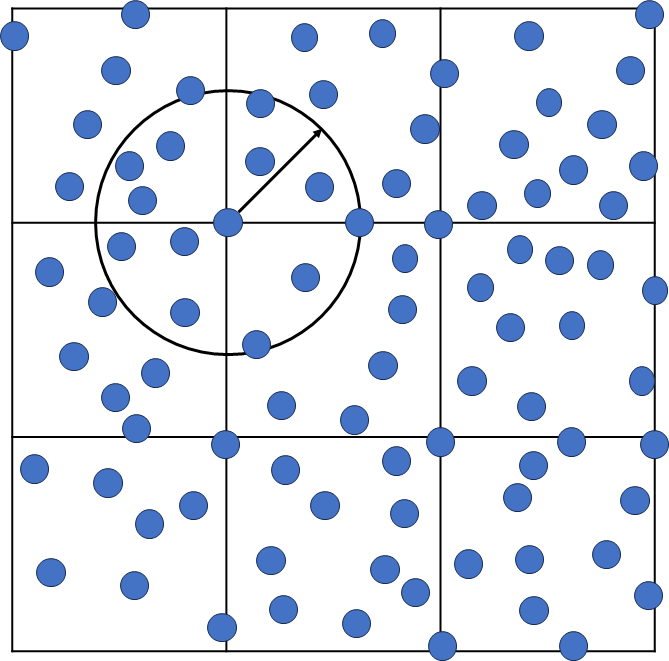
\includegraphics[width=0.5\textwidth]{Methods/Figures/cutoff.png}
        \caption[Representative Image depicting the use of a distance based cut-off scheme for the evaluation of non-bonded interactions]{Representative Image depicting the use of a distance based cut-off scheme for the evaluation of non-bonded interactions. Blue spheres indicate Helium atoms, and the black circle indicates the cut-off sphere for the evaluation of non-bonded interactions.}
    \end{figure}
    
    Here, the distance-based cut-off would be a sufficiently reasonable approximation in the evaluation of short-range VdW interactions, however for long-range interactions such as electrostatics, this approximation would introduce large errors in the evaluated energies due to the slow onvergence. One method to mitigate this problem is the use of Ewald summation, wherein the electrostatic interactions is decomposed into two terms: one term in real-space that converges very quickly, and a long-range term summing over the periodic images. However, Ewald summation might face convergence issues, if either the unit cell is ill-defined, or the unit-cell is not charge neutral. 
    
    In Particle Mesh Ewald (PME) method, the electrostatic interaction is again decomposed into two terms: a short-range term evaluated in real-space, and a long-range term evaluated in fourier space. In PME, the long-range term is evaluated on a discrete mesh of charges, and is evalued using FFT algorithms. As in the case of Ewald summation, PME also requires the simulation to be periodic in x-,y- and z-directions, and have a smoothly varying density.
    
    \subsection{Periodic Boundary Conditions}
    It is computationally impractical to perform MD simulations on systems of experimentally relevant dimensions. Periodic boundary conditions (PBC) allow us to use a simulation box of computationally trackable dimensions and mitigate finite box effects like self-interactions. Under periodic boundary conditions, any particle leaving the box during the simulation is replaced by its image from one of the twenty-six periodic images generated around the original simulation box. We present a representative image depicting the PBC conditions in a 2D plane in Figure 2.2.

    \begin{figure}[!h]
        \centering
        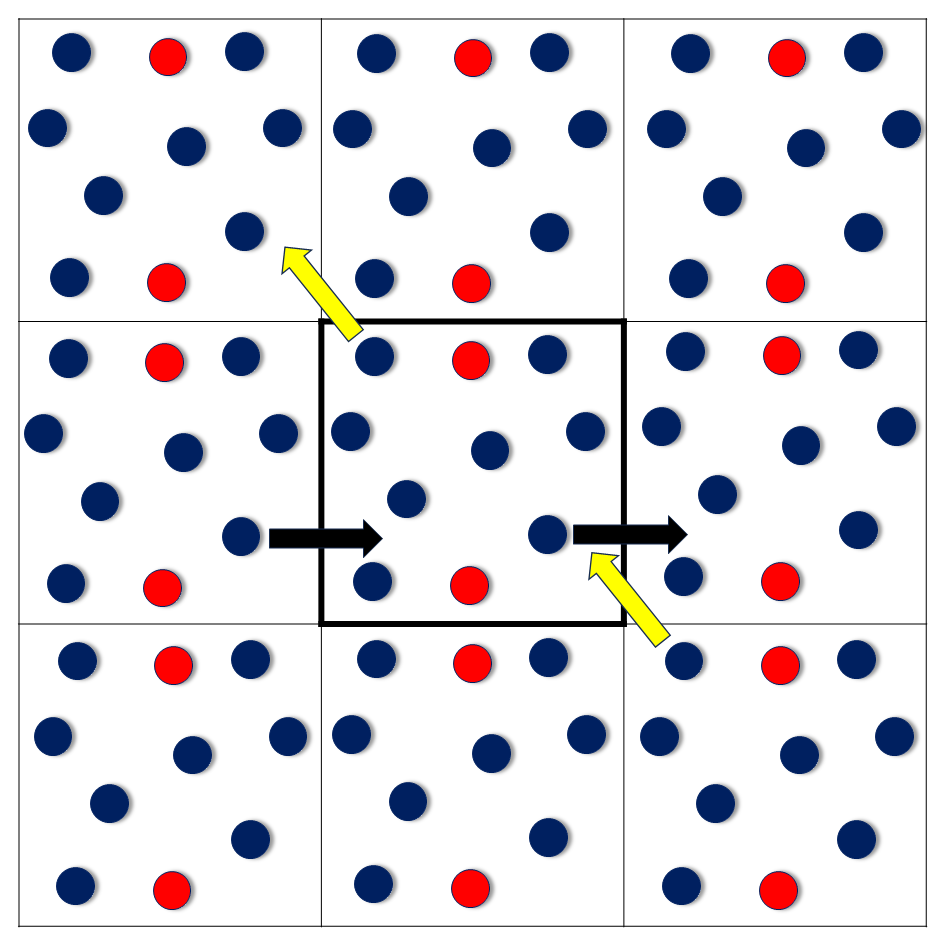
\includegraphics[width=0.5\textwidth]{Methods/Figures/pbc.png}
        \caption[Representative image depicting the application of PBC in a 2D plane]{Representative image depicting the application of PBC in a 2D plane. The central simulation box is indicated by the use of solid lines. The trajectory for two particles at the edges of the simulation box, and its periodic images are also indicated.}
    \end{figure}

    % Consider the case of a 3D system with system dimensions of Lx, Ly and Lz and angles of 90. A naive implementation for the periodic boundary conditions in Fortran, in this case, would be as follows:
    % \begin{align*}
    %     r &= r - r_{old}        \\           
    %     r &= r - \text{ANINT}( \frac{r}{box}) * box \\
    % % r &= r + r_{old}               \\    
    % \end{align*}

    % Here $r$ and $r_{old}$ are the coordinates of the particle at time $t+1$ and $t$, and ANINT is a Fortran routine that rounds a floating point number to the nearest integer.

    \section{Force fields}
    The fundamental idea behind FFs is to decompose the interactions between collections of atoms into a set of analytic functions fitted to reproduce QM results and (or) experimental observables. We can decompose the interactions between sets of atoms into the following sections:
    \begin{itemize}
        \item We model all atoms as hard spheres, and Hook's law models the bonds between atoms, where the bond is approximated with a spring of a specified spring constant, empirically determined. 
        \item We use Hook's law to model angles between three bonded atoms, where the spring constant determines the flexibility of the angle and is also empirically determined. 
        \item We use a periodic potential to model the dihedral between four bonded atoms since the dihedral angle is between [0,180]. 
        \item The standard Lennard-Jones equation evaluates non-bonded interactions between all pairs of non-bonded atoms.
    \end{itemize}
    One central assumption is that the parameters are molecule-agnostic, i.e. the parameters developed for one set of atoms can be transferred with minimal reparameterization towards another molecule, provided the chemical environment of the atom is equivalent. In other words, the parameters used to describe a carbon atom in benzene must be transferrable to describe the carbon atom in naphthalene in a similar chemical environment, with the parameters requiring minimal modifications.
    
    We have employed Chemistry at HARvard Molecular Mechanics (CHARMM) FF for the simulations reported in this thesis. The functional form of the classical non-polarizable additive FF is as follows:
    \begin{multline*}
        V(r^N) = \sum_{bonds}^{}k_i(x_i-x_i^{min})^2 + \sum_{angles}^{}k_j(\theta_j-\theta_j^{min})^2 + \sum_{dihedrals}^{}k_{\phi}(1 + cos(n\phi-\delta)) + \\ \sum_{impropers}^{} k_{\omega}(\omega - \omega_{min})^2 + \sum_{UreyBradley}^{}(S-S_{min})^2 + \\ \sum_{electrostatic}^{}\frac{1}{\epsilon}*\frac{q_i * q_j}{r_{ij}} +  \sum_{VdW}^{}\epsilon_{ij}(\frac{\sigma_{ij}^{12}}{r_{ij}^{12}}-\frac{\sigma_{ij}^{6}}{r_{ij}^6})
    \end{multline*}
    
    where $k_i$, $k_j$ etc are the spring constants for the bonds and angles respectively. Values indicated as $x_{i}^{min}$, $\theta_{i}^{min}$ correspond to the equilibrium bond length and angle. As observed from the equation, the dihedral energy is expressed as the linear combination of a periodic cosine function, where $k_{\phi}$ is the force constant, $\phi$ is the dihedral angle, $\delta$ is the phase shift, and $n$ is the multiplicity of the dihedral. Improper dihedrals are important in maintaining the planarity of a structure, where $k_{\omega}$ is the spring constant and $\omega$ characterizes the out-of-plane bend of the plane. Urey-Bradley interactions account for the 1-3 interactions between the $i^{th}$ and $k^{th}$ atoms in an angle formed by i, j and k atoms, and has important applications in maintaining the geometry of H-O-H angle in water. VdW interactions between two non-bonded atoms i and j, separated by a distance $R_{ij}$ is evaluated using a pairwise Lennard-Jones potential dependent on the specific ``well-depth'' $(\epsilon)$ and equilibrium distance $\sigma$ for the interating particles. The energy terms are evaluated using the standard Lorentz-Berthelot mixing rules:
    \begin{align*}
        \sigma_{ij} &=   \frac{\sigma_i + \sigma_j}{2} \\
        \epsilon_{ij} &= \sqrt{\epsilon_i*\epsilon_j}
    \end{align*}

    Electrostatic energy is computed using Coulumb potential, with $q_i$ and $q_j$ being the partial charges on the particles, and $r_{ij}$ being the distance between the particles.

    \subsection[Classical Drude FF]{Classical Drude FF}
    We have also used classical Drude polarizable FF to investigate the influence of polarizability on the dynamics of the systems. Here, we note that classical non-polarizable FFs like CHARMM have their basis in fixed-point charges, which means that they are not particularly suited for studying systems where significant shifts in the local environment for the molecules are expected, like in the case of biological systems. In such cases, polarizable FFs like classical Drude polarizable FF offers a pathway towards the inclusion of the contributions from the local environment towards the dynamics of the systems.

    In the case of classical Drude polarizable FF, the polarizability of the heavy atoms (excluding hydrogen) is modelled via Drude particles attached to the heavy atoms via a harmonic spring. The Drude particles have a negative charge associated with them. In contrast, the atomic cores have a positive charge, such that the total charge of the atom and associated Drude particle equals the partial charge of the atom. A representative structure depicting the arrangement of atomic cores and associated drude particles are presented in Figure 2.3. 
    \begin{figure}
        \centering
        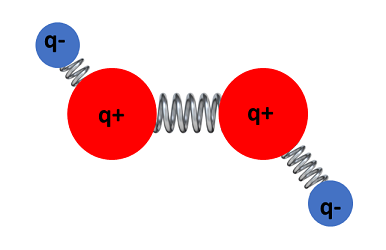
\includegraphics[width=0.75\textwidth]{Methods/Figures/drude.png}
        \caption[Schematic Representation of Drude particles for a C-C bond]{Schematic Representation of Drude particles for a C-C bond. Carbon atoms are represented as red speheres, and Drude particles are represented as blue spheres. The partial positive and negative charges of the heavy atoms and the Drude particles are also indicated. Bonds between heavy atoms are represented as larger springs, and bonds between Drude particles and heavy atoms are represented using smaller springs.}
    \end{figure}

    Here, the Drude particles represent the electronic degrees of freedom for the heavy atom, with the vibration of the Drude particle allowing the electronic interactions of the heavy atom to respond to fluctuations in the local environment, via dipole-dipole and induced-dipole effects. In classical Drude FF, the charges on the Drude particles ($q_D$) and the induced dipole moment ($\mu$) in an external electric field \textit{E} is defined as:
     \begin{align*}
        \mu &= \frac{{q_D}^2 E}{k_d}\\
        d &= \frac{q_D E}{k_d}
     \end{align*}

     We evalue the atomic polarizability ($\alpha$) as:
     \begin{equation*}
        \alpha  =   \frac{{q_D}^2}{k_d}
     \end{equation*}

    Here, the value of $k_D$ corresponds to the harmonic spring constant for the bond connecting the Drude particle to the heavy atom, and has a value of 1000 kcal mol\textsuperscript{-1} for all Drude particle-heavy atom pairs, while a value of 500 kcal mol\textsuperscript{-1}, corresponding to $\frac{k_D}{2}$ is used in CHARMM and NAMD.

    The bonded and non-bonded terms in classical Drude FF is treated exactly the same as in non-polarizable additive FF, with the functional form of the interactions remaining the same in both the FF. The electrostatic interactions are calculated using the following functional form, to include the effects of the electrostatic interactiosn between the unscreened charges, and the Drude particles on $i^{th}$ and $j^{th}$ atom. 
    \begin{align*}
        U_{elec} = \sum_{i}^{}\sum_{j>i}^{}\left[\frac{q_i * q_j}{|r_i - r_j|} + \frac{q_i * q_{D_j}}{|r_i - r_j - d_j|} + \frac{q_j * q_{D_i}}{|r_j - r_i - d_i|} + \frac{q_{D_i} * q_{D_j}}{|r_i - d_i - r_j - d_j|}\right]
    \end{align*}

    Here, $q_i$ and $q_j$ correspond to the unscreened charges on the heavy atoms, while $q_{D_i}$ and $q_{D_j}$ correspond to the charges on the corresponding Drude particles. $r_i$, $r_j$, $d_i$ and $d_j$ are the locations of the $i^{th}$ and $j^{th}$ heavy atoms and the associated Drude particles. The electrostatic term includes the induced-dipole interaction between the two interacting atoms, and 1-2 and 1-3 atom interactions are scaled according to the Thole scaling function, which is described below:
    \begin{align*}
        S_{ij}(r_{ij}) = 1 - \left| 1 + \frac{(a_i * a_j)*r_{ij}}{2(\alpha_i*\alpha_j)^{\frac{1}{6}}}*\exp{\left[\frac{(a_i * a_j)*r_{ij}}{(\alpha_i * \alpha_j)^{\frac{1}{6}}}\right]} \right|
    \end{align*} 

    Here, $r_{ij}$ is the distance between the $i^{th}$ and $j^{th}$ atom, and $a_i$ and $a_j$ are the corresponding thole screeing parameters.

    Classical Drude FF has been employed to investigate the dynamics of a wide variety of systems; including carbohydrates\supercite{pandey_drude_2019,kognole_extension_2022}, proteins and nucleic acids; and contains the parameters to describe a large subset of the chemical space including, but not limited to; biomolecules\supercite{baker_development_2011,savelyev_all-atom_2014}, ions\supercite{lin_polarizable_2018}, water\supercite{lamoureux_polarizable_2006}, heteroatom (O-, N- and S-) conatining molecules\supercite{lopes_polarizable_2009,zhu_polarizable_2010,he_polarizable_2013}, linear and branched hydrocarbons\supercite{vorobyov_polarizable_2005} and aromatic compounds\supercite{lopes_polarizable_2007}.

    We also note that the availabity of classical Drude FF in MD simulation packages like CHARMM\supercite{brooks_charmm_1983,brooks_charmm_2009}, NAMD\supercite{phillips_scalable_2005,phillips_scalable_2020} and OpenMM\supercite{eastman_openmm_2010,eastman_openmm_2017} enables the study of large systems of experimental and biological relevance using MD simulations, without the need to use expensive QM/MM or ab-initio dynamics methods.

The quality of a molecular dynamics simulation is highly dependent on multiple factors, in which three factors listed below are of significant importance:
\begin{itemize}
    \item Initial positions of the atoms in the starting structure. If the intial confirmations introduce some biases in the system, it would affect the simulations outcomes, such that all possible states might not get adequately sampled during the simulation.
    \item Parameters used to describe the interactions between the particles (atoms) during the MD simulation, which are used to compute the potential energy surface. If the parameters used are unable to describe certain interactions, the predictions might not be reflective of the experimental observations.
    \item Integrator used to propagate the structure from time step of $t$ to time step of $t+1$. Some integrators might be numerically unstable over large lengths of time, and the errors at each step might get accumulated in the trajectory.
\end{itemize}

\section{Adaptive Biasing Force Simulations}
We employed Adaptive Biasing Force (ABF) simulations to investigate the binding energies of small molecules with the graphene surface in additive and classical Drude FF simulations. Here, we briefly describe the ABF method and then discuss the specific use case given in this thesis.

ABF, at its core, is an importance sampling method\supercite{comer_adaptive_2015}. However, the importance is adaptive, such that the code can automatically adjust the average force to escape kinetic energy traps in the free-energy surface. In ABF, the free energy along a transition coordinate (called a collective variable) is the negative gradient of the potential arising from the average force acting along that transition coordinate ($\xi$). The force acting on the system can be decomposed into two terms: one corresponding to the average force acting on it and the other term accounting for the random force amounting to the fluctuations in all other degrees of freedom for the system. Here, the random force is thought of as a diffusive force, such that the system under investigation evolves diffusively along the path of the potential of the mean force. The adaptive nature of the ABF method lies in the fact that the method requires no information about the free energy surface apriori, and the derivative of the free energy (and the path of diffusion) is estimated on the fly during the simulation. The method accomplishes this by estimating the running average of the instantaneous force acting on the system and applying an equal and opposite external bias, such that the sum of both forces is zero. Since the average applied external bias would converge to zero over time, and the running average of the instantaneous force on the system converges to the average value at equilibrium, the system now has a flat potential energy landscape, where the remaining barriers would be overcome via thermal fluctuations.

Mathematically, the ABF method works by modifying the potential V to resemble a flat energy landscape along the transition coordinate ($\xi$) of our choice, such that $V(x)$ becomes $V(x) - A_t[\xi(x)]$. We then update $A_t$ such that it converges to the free energy $A$, with the difference of an additive constant, as defined by:
\begin{align*}
    \exp(\beta A(z)) = \int_{}^{}\exp\left[-\beta V(x)\right]\delta_{\xi(x)-z}(dx)
\end{align*}
where $\delta_{\xi(x)-z}(dx)dz = dx$.

We now look into the update rule for $A_t$ such that the condition $\lim_{t\to\infty} A_t = A$ holds true. We have the formula
\begin{align*}
    A'(z) &= -\frac{\int F_{\xi}(x)\exp\left[-\beta V(x)\right]\delta_{\xi(x)-z}(dx)}{\int\exp\left[-\beta (x)\right]\delta_{\xi(x)-z}(dx)} \\
    F_\xi &= -\frac{\nabla V.\nabla\xi}{\left| \nabla\xi \right|^2} + \beta^{-1} div\left(\frac{\nabla\xi}{\left| \nabla\xi \right|^2}\right)
\end{align*}

We now note that $A'(z)$ denotes the conditional average of $F_\xi$, and the equation for $A'(z)$ remains true even when the potential is changed to $V(x) - A_t\circ\xi$ for any function $A_t$. Thus, we note that a biasing potential $A_t$ that depends only on the $\xi$, will leave avergaes conditioned by $\xi$ the same. Tthe logic behind ABF method can be summarized as follows:
\begin{align*}
    dx_t &= M^{-1} p_t dt \\
    dp_t &= -\nabla(V - A_t\circ\xi)(x_t)dt - \gamma M^{-1}p_tdt + \sqrt{2\gamma k_BT}dW_t \\
    A'_t(z) &= E\left[F_\xi(x_t)|\xi(x_t)=z\right]
\end{align*}
where $x_t$ and $p_t$ are the position and momentum of the system at time $t$, $M$ is the mass tensor, $k_B$ is the boltzmann constant, and $W_t$ is the Gaussian random process.

It is recommended that the collective variable $\xi$ be split into multiple windows, so that convergence towards the average value is accelerated.

In this thesis, we employed ABF simulations to investigate the potential of mean force for the interactions between the nucleobases and the graphene surface in Chapter3, between monovalent and divalent cations and Cl\textsuperscript{-1} ion with the graphene surface in Chapter5, and between nucleosides and modified nucleotides and graphene surface in Chapter6. In all these calculations, the collective variable $(\xi)$ was chosen to be the z-projected distance between the graphene surface and the center of mass of the small molecule (nucleobases, nucleosides or modified nucleotides) or ions.

\section{Software and Hardware Used}
This thesis employed the Nanoscale Molecular Dynamics (NAMD) simulation package to perform all classical MD simulations. The initial QM calculations reported in the first chapter used Gaussian 09 and Orca. Home-developed Python codes were also utilized to conduct all the analyses reported herein. All MD trajectories and PDB structures were visualized using the Visual Molecular Dynamics (VMD) and GaussView packages. This thesis required extensive computational resources provided by the High-Performance Computing Facility, IIT Gandhinagar, and Param Ananta Supercomputing Facility at IIT Gandhinagar. 
    \chapter[Polarization Influences the Evolution of Nucleobase -  Graphene Interactions]{Polarization Influences the Evolution of Nucleobase -  Graphene Interactions \protect\footnote[2]{This chapter has been published as \textbf{H., Hemanth} and Mallajosyula*, S.S.; Polarization Influences the Evolution of Nucleobase - Graphene Interactions; {\textit{Nanoscale}, 2021, \textbf{13}, 4060 - 4072}}}
\section{Introduction}
Graphene, a two-dimensional allotrope of carbon with hexagonal lattice has found applications in a wide range of disciplines, with electronics and material science applications at one end of the spectrum and biomedical applications at the other end.\supercite{geim_rise_2007, geim_graphene_2009, lalwani_two-dimensional_2013, akinwande_large-area_2015}  Recently, self-assembly of nucleobases on a solid support has been extensively studied in the literature, with examples of nucleobases spontaneously forming higher-order structures on metal supports like Au(111)\supercite{kelly_understanding_2008, lukas_adenine_2009} Graphene presents itself as a unique support, which can facilitate the self-assembly of nucleobases. In fact, the self-assembly of guanine nucleobases on Graphene Oxide (GO) has been studied in the literature.\supercite{chiorcea_afm_2005} The major advantage of graphene is that it can be used as an atomistically thin monolayer support to study the self-assembly of nucleobases, unlike the surface-driven assembly observed on Au(111) and Ag(111). Graphene has attracted attention as a fast and reliable tool for DNA sequencing\supercite{heerema_graphene_2016, wells_assessing_2012, dontschuk_graphene_2015, schneider_tailoring_2013} through nanopores created within the graphene sheet. Such applications are based on the non-covalent interactions present between the nucleobases and the graphene sheet, and understanding them is relevant for tuning the interactions and successfully creating nanopore based sequencing technology. Expensive QM calculations,\supercite{umadevi_quantum_2011, cho_noncovalent_2013, gowtham_physisorption_2007, umadevi_noncovalent_2014, lee_physisorption_2013} coupled with experimental studies,\supercite{varghese_binding_2009} have been employed to study the binding energies and relative orientations of the nucleobases on the graphene sheet. Multiple authors have shown that polarizability\supercite{gowtham_physisorption_2007, lee_physisorption_2013} of nucleobases play an essential role in dictating the strength of such non-covalent interactions. Computational complexities of routine QM methods such as MP2, HF and DFT which scale as O(\textit{N\textsuperscript{5}}), O(\textit{N\textsuperscript{4}}) and O(\textit{N\textsuperscript{3-4}}) respectively, limit the applicability of QM studies to smaller systems, typically one nucleobase/nucleotide interacting with a patch of the graphene sheet in a gas phase environment. This problem becomes even more challenging upon the inclusion of an explicit solvent in the calculation.

Molecular Dynamics (MD) simulations offer a viable alternative to this scenario, at the cost of high accuracy. At present, MD simulations are routinely employed to study the time evolution of large systems and help in understanding the dynamics of such systems. However, additive Force Fields (FFs) based on fixed point charges used to describe the interactions (bonded and non-bonded) in MD simulations are ill-equipped to describe the time evolution of molecular polarizability of the system. The results from MD simulations based on additive FF suggest that a subtle interplay between intermolecular hydrogen-bonding and $\pi$-$\pi$ interactions between nucleobases and the graphene sheet decides the outcome of nucleobase - graphene sheet interactions.\supercite{saikia_hierarchical_2017, saikia_dynamics_2018, ortmann_attracted_2005} However, a full-scale investigation based on the polarizable FF is absent from the literature. In this regard, we study the dynamics of nucleobases in the presence of a polarizable graphene sheet, to understand the effect of molecular polarizability on non-covalent interactions, by employing a Drude polarizable FF available in Chemistry at Harvard Molecular Mechanics (CHARMM).
\section{Computational Methodology}
Geometry optimizations for coronene were performed using the Gaussian 09 suite of programs, at the MP2/6-31G(d) level of theory. Vibration modes were also calculated at the same level of theory to ensure that the molecule was at a minimum on the potential energy surface.  Interaction energies were calculated using the ORCA suite of programs,\supercite{neese_orca_2012} at the RI-MP2/cc-pVQZ/cc-pVQZ/C level of theory from geometries optimized at the MP2/6-31G(d) level of theory. QM calculations were used to test the transfer of parameters.
\begin{figure}
    \centering
    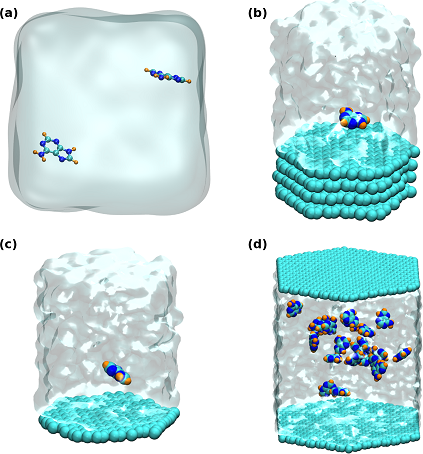
\includegraphics{Chapter1/Figures/Figure1.png}
    \caption[Representative structures for the systems considered in the present study]{Representative structures for the systems considered in the present study. (a) Free-standing nucleobases (b) Graphene - nucleobase PMF calculations using ABF simulations with multilayer graphene sheet, (c) Graphene -  nucleobase PMF calculations using ABF simulations with monolayer graphene sheet and (d) Homogeneous nucleobase- graphene system}
    \label{fig:figure17}
\end{figure}

The MD simulations were performed at the isobaric-isothermal (NPT) ensemble using the Nanoscale Molecular Dynamics (NAMD) package.\supercite{phillips_scalable_2005} CHARMM36 all-atom force field was used to describe the bonded and non-bonded interactions in graphene and nucleobases in additive FF simulations. Classical Drude polarizable FF was employed to describe the bonded and non-bonded interactions in nucleobases for Drude polarizable FF simulations. Parameters developed in-house were used to describe the bonded and non-bonded interactions in the polarizable graphene sheet. Particle Mesh Ewald (PME)\supercite{darden_particle_1993} summation was used to evaluate the electrostatic interactions with a cut-off of 9.0 $\angstrom$. Water molecules were described by the TIP3P\supercite{jorgensen_comparison_1983} water model in additive FF simulations, and the SWM4-NDP\supercite{lamoureux_polarizable_2006} polarizable water model was employed in the Drude polarizable FF simulations, with bond lengths and bond angles constrained via the SETTLE algorithm.\supercite{miyamoto_settle_1992} All simulations were performed at room temperature (298 K) with Langevin dynamics using the Nos\'{e}-Hoover Langevin piston method applied to maintain the pressure at 1 atm. For Drude FF simulations, an additional dual thermostat was employed to maintain the Drude particles in an ice bath at 1 K.

Free-standing nucleobases were modelled using CHARMM for additive FF simulations and the solvated system was simulated in a box of dimensions (30 × 30 × 30)$\angstrom$\textsuperscript{3}. We present a representative structure depicting the system setup for free-standing nucleobases in Figure 3.1(a).  Corresponding input files for the Drude polarizable FF were generated using in-house scripts. All systems were minimized with 60000 steps of CG minimization, and subsequent equilibration for 1 ns in the NPT ensemble. Production runs for additive FF simulations were run for 800 ns, while for the Drude polarizable FF simulations, production simulations were run for 2300 ns for adenine, 500 ns for guanine and thymine, and 2000 ns for cytosine. The simulations for adenine and cytosine were extended from 500 ns to 2300 ns and 2000 ns to achieve convergence.

Simulations using Adaptive Biasing Force (ABF) were also performed to estimate the binding free energies for nucleobase - nucleobase interactions and nucleobase - graphene sheet interactions. We employed a biasing force of 0.20 kcal mol\textsuperscript{-1}$\angstrom$\textsuperscript{-2} at both ends of the scan length. The scan length was divided into windows of length 0.05 $\angstrom$. We employed two methodologies to perform the ABF simulations. The first methodology was adapted from the work by Comer et al.\supercite{comer_predicting_2015,poblete_determinants_2017} In this methodology, four layers of graphene sheets were constructed to simulate a bulk graphite, with the lower sheets restrained by applying a harmonic potential. Nucleobases were placed on top of the graphene sheet and ABF simulations were performed. The ABF simulations were performed in a hexagonal unit cell of dimensions (29 x 29 x 45)  $\angstrom$\textsuperscript{3}. We present a representative structure depicting the system setup for the ABF simulations with the bulk graphite in Figure 3.1(b). In the second methodology, the ABF simulations were performed using a monolayer of graphene, to differentiate graphene and the bulk graphite. A monolayer graphene system was constructed as a hexagonal unit cell of dimensions (29 x 29 x 30) $\angstrom$\textsuperscript{3}. We present a representative structure depicting the system setup for ABF simulations with a monolayer graphene in Figure 3.1(c). Similar to the four-layer graphite system, the nucleobase was placed atop the graphene sheet. ABF scans in a nucleobase - nucleobase system were performed from 3 $\angstrom$ to 10 $\angstrom$. ABF scans in a nucleobase - graphene sheet system were performed from 3 $\angstrom$ to 15 $\angstrom$. ABF simulations for both systems were run for 100 ns in both additive and Drude FF. The simulations were deemed to have attained convergence when the number of observations in each bin was >1.5 x 10\textsuperscript{6}.

The graphene sheet was modeled using Inorganic Builder Toolkit available in VMD,\supercite{humphrey_vmd_1996} with a radius of 21 $\angstrom$ and a height of 2 $\angstrom$. We used 21 nucleobases for homogeneous nucleobase - graphene sheet simulations, and 30 nucleobases (15 of each type) in heterogeneous nucleobase - graphene sheet simulations.The graphene sheet-nucleobase system was simulated in a hexagonal unit cell of dimensions (52 × 52 × 60) $\angstrom$\textsuperscript{3}.  We present a representative structure depicting the system setup for the homogeneous nucleobase - graphene sheet simulations in Figure 3.1(d).  All systems were minimized with 60000 steps of CG minimization, and subsequent equilibration for 1 ns in the NPT ensemble. Production simulations were run for 500 ns in the NPT ensemble for additive FF, and for 500 ns in Drude FF. The equations of motion were integrated with a time step of 2 fs in additive FF simulations, while a shorter time step of 1 fs was employed in Drude polarizable FF simulations. The central atom in the graphene sheet was restrained using a harmonic potential, to ensure that the sheet does not slide during the simulations. No additional constraints were applied, and the sheets were allowed to breathe during the simulations. We note that there are a lot of reports in the literature in which the complete sheet geometry is constrained. We have ensured that the parameters allow for the ``breathing'' motion of the graphene sheets. 

Hydrogen bond and dipole moment analysis was performed using plugins available in VMD. The average number of hydrogen bonds present in the system serves as an indicator of the overall stability of the system, with a higher number of hydrogen bonds suggesting the presence of ordered structures within the system. Instances of $\pi$-$\pi$ interactions between (1) nucleobases and (2) nucleobase - graphene sheets were tracked with in-house analysis codes. Relative orientations of the nucleobases with respect to the graphene sheet were tracked to establish preferential conformations of the nucleobases in the simulation box.

\section{Results and Discussions}
\subsection{Validation of transferred parameters for the polarizable graphene sheet}
\begin{table}
	\centering
	\caption[Tansferred classical Drude Polarizable FF parameters]{Parameters transferred from benzene to graphene sheet in Drude polarizable FF. The atom descriptors are presented in Figure 3.3.}
	\begin{tabular}{cccc}
            \toprule
		Identifier	&	Parameter & Force Constant & Multiplicity\\ \midrule
		$l_{C-C}$ ($\angstrom$)	&	1.375	& 305.000&	--\\
		$l_{C-H}$ ($\angstrom$)	&	1.080	& 340.000&	--\\
        $\theta_{CCC}$(\degree)	&	120.00& 40.000& --\\
		$\theta_{CCH}$ (\degree)	&	120.00& 30.000 &--\\
		$\phi_{CCCC}$(\degree)	&	180.00  &  2.800&    2 \\
		$\phi_{CCCH}$ (\degree)	&	180.00& 4.200    &2\\
		$q_{C^\#}$	(e)&	0.0000& --&--\\
		$q_{C^\dagger}$	(e)&	0.0000& --&--\\
		$q_{C^\ddagger} $	(e)&	-0.1106& --&--\\
		$q_{H}$	(e)&	0.1106&-- &--\\
		$k_D$ (kcal/mol/$\angstrom^2$)	&	1000& --&--\\
		$\epsilon_C$ (kcal/mol)	&	-0.0690&-- &--\\
		$\sigma_C$ ($\angstrom$)	&	2.0900&-- &--  \\ \bottomrule
	\end{tabular}
 \end{table}
 
\begin{figure}
    \centering
    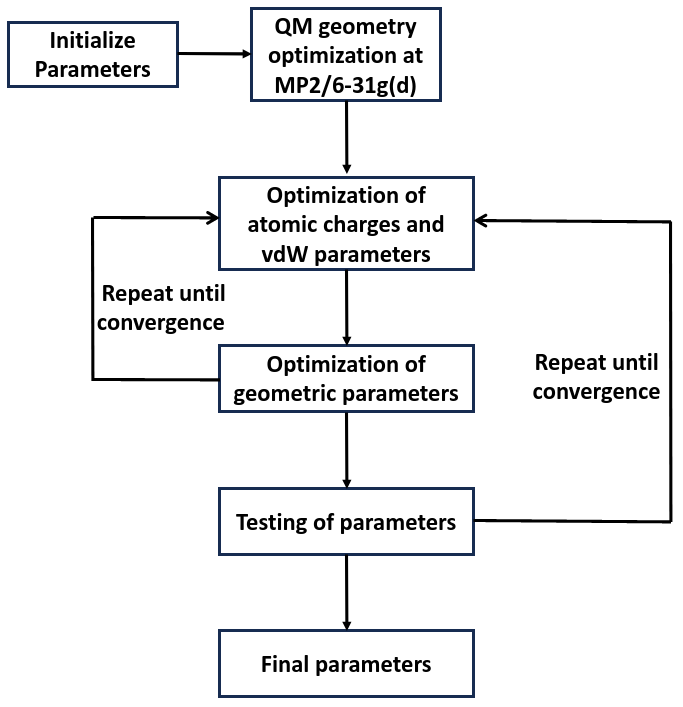
\includegraphics[width=0.6\textwidth]{Chapter1/Figures/Scheme-final.png}
    \caption[Parameterization strategy in CHARMM FF]{Parameterization strategy in CHARMM FF.}
\end{figure}

\begin{figure}
    \centering
    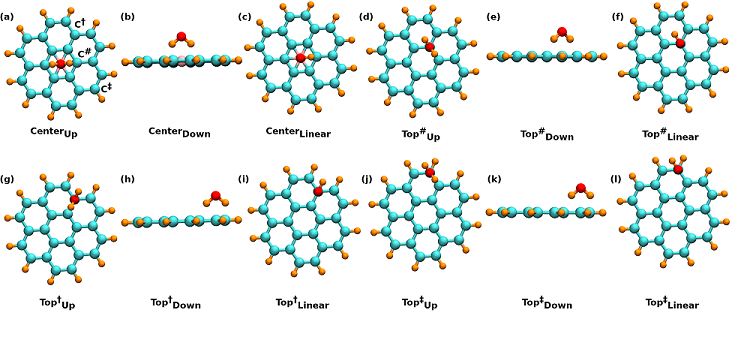
\includegraphics{Chapter1/Figures/water.png}
    \caption[Different solute-water pair interaction modes for the coronene - water model system]{Different solute-water pair interaction modes for the coronene - water model system. Carbon atoms are colored green, oxygen atoms are red and hydrogen atoms are orange. (a), (c), (d), (f), (g), (i), (j) and (l) present the top view of the concerned system, while (b), (e), (h) and (k) present the side views of the systems. C\textsuperscript{\#} forms the central six-membered ring of coronene. C$^\dagger$ corresponds to the carbon atoms on the peripheral ring, connected to the hydrogen atoms. C$^\ddagger$ corresponds to the carbon atoms on the periphery, not connected to the hydrogen atoms. All figures are generated using VMD.}
\end{figure}

The absence of suitable parameters to describe a polarizable graphene sheet necessitated the development and testing of new FF parameters to describe the graphene sheet. Towards this end, we transferred the parameters available in CHARMM Drude polarizable FF for polarizable benzene to model a polarizable graphene sheet. This transfer is analogous to the transfer of parameters from benzene to model graphene in the additive FF. The transferred parameters are presented in Table 3.1. The strategy employed for the testing of transferred parameters is presented Figure 3.2. The transferred parameters were tested using coronene as a model system for graphene, with the central six-membered ring analogous to carbons in the graphene sheet, and the external ring being analogous to the passivated ends and central pore. The transferred parameters were tested to capture the water interactions with coronene. Eight different interaction modes were considered for studying the interaction of the water molecule with the graphene sheet, which can be classified as Center, Top\textsuperscript{$\dagger$}, Top\textsuperscript{$\ddagger$} and Top\textsuperscript{\#} based on the interacting carbon atom and Up or Down based on the orientation of hydrogen atoms in the water molecule. The interaction geometries considered were based on the previous study by Schyman et al. where the adsorption of water molecules and ions was explored using OPLA-AAP FF,\supercite{schyman_exploring_2013} where it was shown that the linear approach by water molecules was disfavoured in larger carbon-based aromatic structures. All interaction modes considered are presented in Figure 3.3. The solute-water pair distances and interaction energies obtained from the QM and MM (Drude) calculations are presented in Tables 3.2 and 3.3. The interaction energies are evaluated as $E$(interaction energy) = $E$(coronene + water) - $E$(coronene) - $E$(water). These have been reported as $E$\textsubscript{QM} and $E$\textsubscript{MM}(Drude) in Table 3.3. We observed a fair reproduction of the solute-water pair interaction distances and interaction energies by the transferred parameters. The strongest interactions were observed when the water molecule approaches coronene with the hydrogens facing the sheet. The solute-water pair interaction energies calculated using RI-MP2 are also shown in Table 3.3. The parameters showed good agreement with the values obtained from QM calculations at the MP2/6-31G(d)//RI-MP2/cc-pVQZ/cc-pVQZ/C level of theory. The interaction energies and solute-water distances were also calculated at the $\omega$-B97X-D level of theory to ensure that the developed parameters are able to closely reproduce the previously reported water-interaction energy and distance reported for the system in polarizable version of the Optimized Potentials for Liquid Simulations-All Atom (OPLS-AAP) FF.

To test the applicability of the parameters developed for the polarizable graphene sheet, we calculated the binding free energies of the nucloebases to test the ability of the parameters to suitably reproduce the binding energy profiles calculated from additive and gas-phase QM simulations.

% \begin{algorithm}
%     \caption[Parameterization strategy in CHARMM FF]{Parameterization strategy in CHARMM FF.}
%     \begin{algorithmic}
%         \State Parameters $\gets$ Initialize parameters based on chemical similarity.
%         \State QM geometry $\gets$ QM geometry optimization at MP2/6-31g(d) level of theory.
%         \State QM water interaction $\gets$ QM water interactions at MP2/6-31g(d) level of theory.
%         \While{Not converged}
%             \State Optimize atomic charges and vdW parameters [Intermolecular parameters]
%             \State Optimize geometric parameters [Intramolecular parameters] 
%             \State Check convergence for both intermolecular and intramolecular parameters.
%         \EndWhile
%         \State Parameters $\gets$ Final (Optimized) FF parameters.
%     \end{algorithmic}
% \end{algorithm}

%  \begin{landscape}
    \begin{table}
        \centering
        \small
        \caption[Solute-water pair distances for the coronene - water interaction modes]{Solute-water pair distances for the coronene - water interaction modes. All distances are reported in \angstrom. MM\textsubscript{D} represents the Drude polarizable FF simulations}
            \begin{tabularx}{\textwidth}{ccccccc}
                \toprule
                Interaction                 &   MP2     &   $\omega$-B97X-D     &   MM\textsubscript{D}     &   QM\textsubscript{MP2}-MM\textsubscript{D}   &   QM\textsubscript{$\omega$-B97X-D}-MM\textsubscript{D}   &   OPLS-AAP \supercite{schyman_exploring_2013}  \\ \midrule
                Center\textsubscript{Up}    &   2.94    &   3.00    &   3.42    &   -0.48   &   -0.42   &   --  \\
                Top\textsuperscript{\#}\textsubscript{Up}   &   3.06    &   3.09    &   3.54    &   -0.48   &   -0.45   &   --  \\
                Top\textsuperscript{$\dagger$}\textsubscript{Up}    &   3.21    &   3.24    &   3.64    &   -0.43   &   -0.40       &   --  \\
                Top\textsuperscript{$\ddagger$}\textsubscript{Up}    &   3.32    &   3.29   &   3.60   &   -0.28  &   -0.31       &   --  \\ 
                Average\textsubscript{Up}   &   3.13    &   3.16    &   3.55    &   -0.42   &   -0.40   &   --  \\
                Center\textsubscript{Down}  &   3.20    &   3.27  &   3.36  &   -0.16 &   -0.09   &   3.15  \\
                Top\textsuperscript{\#}\textsubscript{Down} &   3.26    &   3.30    &   3.42    &   -0.16   &   -0.12   &   --  \\
                Top\textsuperscript{$\dagger$}\textsubscript{Down}  &   3.32    &   3.37    &   3.46    &   -0.14   &   -0.09   &   --  \\
                Top\textsuperscript{$\ddagger$}\textsubscript{Down} &   3.32    &   3.35    &   3.44    &   -0.12   &   -0.09   &   --  \\ 
                Average\textsubscript{Down}   &   3.28    &   3.32  &   3.42  &   -0.15 &   -0.10       &   3.15    \\  \bottomrule        
            \end{tabularx}
        \label{tab:my_label}
    \end{table}

    \vspace{2em}
    
    \begin{table}
        \centering
        \small
        \caption[Solute-water pair interaction energies for the coronene - water interaction modes]{Solute-water pair interaction energies for the coronene-water interaction modes. All energies are reported in kcal mol\textsuperscript{-1}. $\Delta{E}$\textsuperscript{1} = $E$\textsubscript{MM}-$E$\textsubscript{MP2}, $\Delta{E}$\textsuperscript{2} = $E$\textsubscript{MM}-$E$\textsubscript{$\omega$-B97X-D}, $\Delta{E}$\textsuperscript{3} = $E$\textsubscript{MM}-$E$\textsubscript{RI-MP2}}
            \begin{tabular}{cccccccc}
                \toprule
                Interaction                 &   $E$\textsubscript{MP2}     &    $E$\textsubscript{$\omega$-B97X-D}  &   $E$\textsubscript{RI-MP2}   &   $E$\textsubscript{MM}   &   $\Delta{E}$\textsuperscript{1}  &   $\Delta{E}$\textsuperscript{2}  &   $\Delta{E}$\textsuperscript{3}  \\ \midrule
                Center\textsubscript{Up}    &   0.15    &   -0.81   &   -1.59   &   -0.82   &   -0.97   &   -0.01   &   0.77    \\
                Top\textsuperscript{\#}\textsubscript{Up}   &   0.45  & -0.36 & -1.13 & -0.56 & -1.01 & -0.20 & 0.57 \\
                Top\textsuperscript{$\dagger$}\textsubscript{Up}   &    0.69  & 0.17  & -0.55 & -0.38 & -1.07 & -0.55 & 0.17  \\    
                Top\textsuperscript{$\ddagger$}\textsubscript{Up}   &   0.57  & 0.11  & -0.39 & -0.47 & -1.04 & -0.58 & -0.08  \\    
                Average\textsubscript{Up}   &   0.47  & -0.22 & -0.92 & -0.56 & -1.02 & -0.34 & 0.36    \\  
                Center\textsubscript{Down}    & -2.35 & -4.00 & -3.77 & -3.12 & -0.77 & 0.88  & 0.65    \\
                Top\textsuperscript{\#}\textsubscript{Down}   & -2.20 & -3.82 & -3.48 & -2.88 & -0.68 & 0.94  & 0.60 \\
                Top\textsuperscript{$\dagger$}\textsubscript{Down}   &  -1.71 & -3.15 & -2.70 & -2.32 & -0.61 & 0.83  & 0.38  \\    
                Top\textsuperscript{$\ddagger$}\textsubscript{Down}   & -1.49 & -2.92 & -2.44 & -1.91 & -0.42 & 1.01  & 0.53  \\    
                Average\textsubscript{Down}   & -1.94 & -3.47 & -3.10 & -2.56 & -0.62 & 0.92  & 0.54  \\    \bottomrule 
            \end{tabular}
        \label{tab:my_label}
    \end{table}
%  \end{landscape}

 \begin{landscape}
    \begin{table}
       \centering
       \small
       \caption[Binding free energies of nucleobases obtained from additive and Drude PMF simulations and QM calculations]{Binding free energies of nucleobases obtained from additive and Drude PMF simulations and QM calculations. All energies are reported in units of kcal mol\textsuperscript{-1}. Additive\textsuperscript{\#} and Drude\textsuperscript{\#}  correspond to PMF calculations on an unconstrained monolayer graphene sheet. Binding free energies are calculated as the difference between the energies of the equilibrium state and well-separated states. Exp. = aqueous solution and Exp.\textsuperscript{\#} = NaOH solution. Difference between the binding energies of 4-layer graphite and monolayer graphene simulations is reported in parentheses.}
       \begin{tabular}{ccccccccccc}
           \toprule
           Nucleobase  &   Additive (c36)  & Drude &   $\Delta{E}$\textsubscript{Add-Drude}    &   Additive\textsuperscript{\#} (c36)  &   Drude\textsuperscript{\#}    &  $\Delta{E}$\textsuperscript{\#}\textsubscript{Add-Drude}   &   QM  &   QM \supercite{antony_structures_2008}  &   Exp.\supercite{varghese_binding_2009}    &   Exp.\textsuperscript{\#}\supercite{varghese_binding_2009} \\ \midrule
           Adenine  & -9.40 & -8.35 & -1.05 & -8.51(-0.89) & -8.61(-0.26) & 0.10 & -17.24 & -13.6 & -6.64 & -11.85 \\
           Guanine  & -9.68 & -9.85 & 0.17  & -8.93(-0.75) & -9.51(-0.34) & 0.58 & -17.23 & -17.6 & —     & -13.45 \\
           Cytosine & -7.03 & -5.96 & -0.31 & -6.86(-0.17) & -7.87(1.91)  & 1.01 & -13.47 & -13.0 & -4.39 & -9.38  \\
           Thymine  & -7.97 & -7.66 & -1.07 & -7.73(-0.24) & -8.27(0.61)  & 0.54 & -14.33 & -14.7 & -0.68 & -4.72  \\
           Uracil   & -7.35 & -7.03 & -0.32 & -6.83(-0.52) & -7.00(-0.03) & 0.17 & -12.20 & -12.6 & —     & —     \\ \bottomrule
       \end{tabular}
       \label{tab:my_label}
    \end{table}   
   
    \begin{table}
        \centering
        \small
        \caption[Binding free energies of nucleobases obtained from additive and Drude PMF calculation for unconstrained and constrained monolayer graphene sheet]{Binding free energies of nucleobases obtained from additive and Drude PMF calculation. All energies are reported in units of kcal mol\textsuperscript{-1}. Additive\textsuperscript{\#} and Drude\textsuperscript{\#} corresponds to PMF calculations in Additive and Drude polarizable FF on an unconstrained monolayer graphene sheet. Add\textsuperscript{$\dagger$} and Drude\textsuperscript{$\dagger$} corresponds to PMF calculations calculations in Additive and Drude polarizable FF on a fully constrained monolayer graphene sheet. Binding free energies are calculated as the difference between the energies of equilibrium state and well separated states.}
        \begin{tabular}{ccccccc}
           \toprule
           Nucleobase  &   Additive\textsuperscript{\#} (c36)  &   Additive\textsuperscript{$\dagger$} (c36)   &   $\Delta{E}$\textsuperscript{\#}\textsubscript{Additive\textsuperscript{\#}-Additive\textsuperscript{$\dagger$}} &   Drude\textsuperscript{\#}   &   Drude\textsuperscript{$\dagger$}    &   $\Delta{E}$\textsuperscript{\#}\textsubscript{Drude\textsuperscript{\#}-Drude\textsuperscript{$\dagger$}}     \\ \midrule
           Adenine  & -8.51 & -9.06 & 0.55 & -8.35 & -8.92 & 0.57  \\
           Guanine  & -8.93 & -9.41 & 0.48 & -9.85 & -9.76 & -0.09 \\
           Cytosine & -6.86 & -6.89 & 0.03 & -5.96 & -6.64 & 0.68  \\
           Thymine  & -7.73 & -8.47 & 0.74 & -7.66 & -6.32 & -1.34 \\
           Uracil   & -6.83 & -7.03 & 0.20 & -7.03 & -6.86 & -0.17 \\ \bottomrule
        \end{tabular}
        \label{tab:my_label}
    \end{table}
 \end{landscape}

 \subsection{Potential of mean force calculations}
 \begin{figure}
    \centering
    \includegraphics{chapter1/Figures/Figure3.png}
    \caption[Representative image for scan coordinate in nucleobase - graphene sheet ABF simulations]{Representative image for scan coordinate in nucleobase - graphene sheet ABF simulations.}
 \end{figure}
 \begin{figure}
    \centering
    \includegraphics{chapter1/Figures/Figure2.png}
    \caption[Potential of Mean Force (PMF) of the five nucleobases: adenine, thymine, guanine, cytosine and uracil, respectively]{Potential of Mean Force (PMF) of the five nucleobases: adenine, thymine, guanine, cytosine and uracil, respectively.}
 \end{figure}
 Potential of Mean Force (PMF) was calculated for the adsorption of the nucleobases (adenine, guanine, thymine, cytosine and uracil) on the graphene sheet to estimate the effect of polarization on the binding free energies. The scan coordinate used for evaluating the nucleobase - graphene sheet PMF is presented in Figure 3.4.  PMF scans obtained from additive, Drude polarizable FF and QM calculations are presented in Figure 3.5. Binding free energies estimated from additive and Drude simulations of the four-layer graphite and monolayer graphene are presented in Table 3.4. The binding free energies from the Drude (additive) simulations from the four-layer graphite ABF simulations for the five nucleobases G, A, T, C and U were found to be -9.85 (-9.68), -8.35 (-9.40), -7.66 (-7.97), -5.96 (-7.03) and -7.03 (-7.35), respectively. The binding free energies from the Drude (additive) simulations from the monolayer graphene ABF simulations for the five nucleobases G, A, T, C and U were found to be -9.51 (-8.93), -8.61 (-8.51), -8.27 (-7.73), -7.87 (-6.86) and -7.00 (-6.83), respectively. All energies are presented in kcal mol\textsuperscript{-1}. We find that the inclusion of polarizability makes it easier to adsorb and desorb nucleobases from the bulk graphite. The binding free energies for A and C are -1.05 kcal mol\textsuperscript{-1} and -1.07 kcal mol\textsuperscript{-1} lower respectively in classical Drude polarizable FF simulations, when compared to the additive simulations for the bulk graphite system. The influence of polarization on G, C and U was minimal when compared to A and T for the bulk graphite system. In terms of the absolute values, the binding free energies follow the trend G > A > T > U > C in both Drude and additive simulations of the bulk graphite systems. For the monolayer systems, the binding energies of C, G and T are 1.01 kcal mol\textsuperscript{-1}, 0.58 kcal mol\textsuperscript{-1} and 0.54 kcal mol\textsuperscript{-1} higher respectively in classical Drude polarizable FF simulations, when compared to the additive simulations. The influence of polarization on A and U was minimal when compared to that on G, C and T for the monolayer graphene system. We find that the inclusion of polarizability makes it harder to adsorb and desorb nucleobases from the monolayer graphene. In terms of the absolute values, the binding free energies follow the trend G > A > T > C > U in both Drude and additive simulations of the monolayer graphene systems. We note that while the inclusion of polarization makes it easier to desorb nucleobases from graphite, the same favours strong adsorption over the monolayer graphene. However, in both the cases, the maximum change is of the order of 1 kcal mol\textsuperscript{-1}. This is in agreement with the experimental observations by Varghese et al.\supercite{varghese_binding_2009}, and theoretical calcultaions by Grimme et al.\supercite{antony_structures_2008} The graphene-nucleobase interaction energies calculated using isothermal titration calorimetry in aqueous (alkaline) solution reported by Varghese et al. for G, A, T and C were found to be nil (-13.45), -6.64 (-11.85), -0.68 (-4.72) and -4.34 (-9.38), respectively (interaction energies could not be calculated for guanine in aqueous solution due to the insolubility of guanine in aqueous solution).  All energies are reported in kcal mol\textsuperscript{-1}. We observe that the values obtained using both the Drude and additive simulations lie between the experimental values obtained for aqueous and alkaline solutions. Additionally, we also performed ABF simulations with a constrained graphene sheet to probe the influence of structural fluctuations in the graphene monolayer on the adsorption of the nucleobases. The binding free energies are tabulated in Table 3.5. For the additive simulations, we observe that the average difference in the binding free energies upon constraining the sheet is 0.4 kcal mol\textsuperscript{-1}. The maximum difference was observed for T with the binding free energy being 0.74 kcal mol\textsuperscript{-1} higher upon constraining the sheet. For Drude simulations, the maximum difference in binding free energies between an unconstrained and constrained sheet was observed for T and C. For T, we observe that constraining the sheet lowered the binding free energy with the difference being -1.34 kcal mol\textsuperscript{-1}, while for C constraining the sheet increases the binding energy with the difference being 0.68 kcal mol\textsuperscript{-1}. From both additive and Drude simulations, we note that constraining the sheet influences the binding energetics and must be accounted for in the simulations.
 
 \subsection{Nucleobase - nucleobase interactions}
 Before studying the interaction of the nucleobases with the graphene sheet, we also estimated the influence of polarization on the nucleobase - nucleobase interactions. We estimated the binding free energies of nucleobase - nucleobase interactions by studying the dynamics of a two nucleobase system via an unbiased simulation and an adaptive biasing force (ABF) simulation. The unbiased simulations were run for 800 ns and 500 ns for the additive and Drude FF, respectively. The simulations for adenine and cytosine were extended to 2300 ns and 2000 ns, respectively, to ensure convergence. In the ABF simulations, the scan coordinate was defined as the distance between the center of mass (COM) of the two nucleobases. In Figure 3.6, we present a representative illustration of the scan coordinate. In Figures A.1 and A.2 of the Appendix A, we present the time series corresponding to the distance between the COM of the two nucleobases and the relative orientation between the two nucleobases for the additive and Drude simulations, respectively. The PMF plots obtained for the nucleobase-nucleobase interactions from the additive and Drude simulations are presented in Figure A.3 in the Appendix A. The structures corresponding to the minima observed from the PMF calculations for nucleobase-nucleobase interactions are presented in Figure 3.7.

    \begin{figure}
        \centering
        \includegraphics{Chapter1/Figures/Figure4.png}
        \caption[Representative image for scan coordinate in nucleobase - nucleobase ABF simulations]{Representative image for scan coordinate in nucleobase - nucleobase ABF simulations. Orientation of nucleobases are  calculated from the normal vectors of molecular planes, as \textit{arccos(NormalI · NormalII)}.}
    \end{figure}

    \begin{table}
        \centering
        \caption[Binding free energies of nucleobase - nucleobase interactions obtained from additive and Drude simulations]{Binding free energies of nucleobase - nucleobase interactions obtained from additive and Drude simulations. All energies are reported in units of kcal mol\textsuperscript{-1}. Binding free energies are calculated as the difference between the energies of the equilibrium state and the well-separated states. Binding energies from the unbiased simulations are reported in parentheses. dA, dC, dT and U correspond to deoxyadenosine, deoxythymidine, deoxycytidine and uridine, respectively.}
        \begin{tabular}{ccccc}
            \toprule
            Nucleobase & additive & Drude\textsubscript{$\pi$-stacking} & Drude\textsubscript{Hbond} & Expt.\supercite{schyman_exploring_2013} \\ \midrule
            Adenine & -1.54(-1.23) & -2.17(-1.20) & -1.50(dA)	& -5.62(-5.02) \\
            Guanine & -1.74(-1.36) & -1.96(-1.75) & - & -1.95(-1.21) \\
            Cytosine & -0.42(-0.09) & 0.66(0.34) & 0.06(dC) & -2.03(-2.59) \\
            Thymine & -0.99(-0.72) & 0.95(-0.29) & 0.06(dT) & -0.57(-0.23) \\
            Uracil & -0.54(-0.69) & -0.61(-0.45) & 0.21(U) & -0.39(-0.21) \\ \bottomrule
        \end{tabular}
    \end{table}

    \begin{figure}
        \centering
        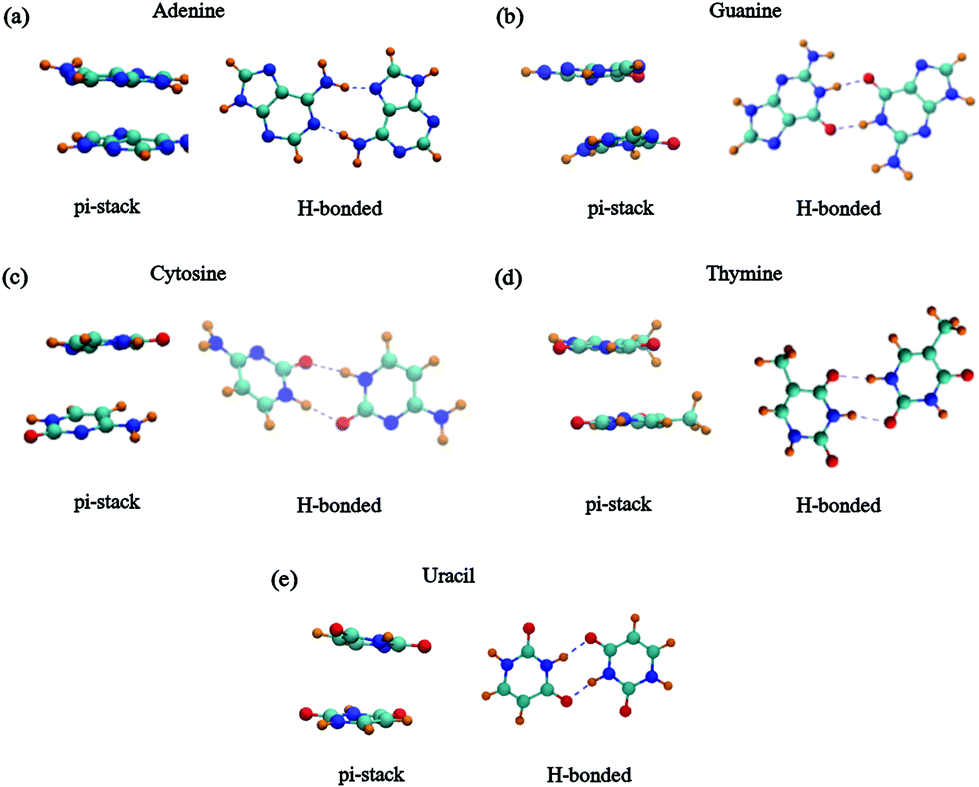
\includegraphics[width=\textwidth]{Chapter1/Figures/Figure6.png}
        \caption[Representative structures corresponding to various minima observed in the PMF curves for Adenine, Guanine, Cytosine, Thymine and Uracil nucleobases.]{Representative structures corresponding to various minima observed in the PMF curves for (a) Adenine, (b) Guanine, (c) Cytosine, (d) Thymine and (e) Uracil nucleobases.}
    \end{figure}

    We observe that adenine forms an unsymmetrical hydrogen-bonded dimer, while other nucleobases favour the formation of symmetrical dimers. It was also observed that all nucleobases were preferentially adopting a slip-stacked arrangement in $\pi$-stacked configurations. We observed a satisfactory overlap between the binding energies obtained from both the unbiased and ABF simulations in both additive and Drude simulations. On comparing the additive and Drude simulations, we also observe distinct signatures of the influence of polarization.  Additive simulations predominantly favor only the $\pi$-stacking conformations for all the nucleobases, while in the Drude simulations, we observe both hydrogen bonding and $\pi$-stacking conformations.  In fact, hydrogen bonding was observed to be the preferred mode of interaction for all the nucleobases, except guanine, where both $\pi$-stacking and hydrogen bonding were equally favoured. Binding free energies for $\pi$-stacking obtained from additive and Drude simulations are presented in Table 3.6. For the additive simulations, we observe that both the ABF and unbiased simulations predict the binding free energy trend as G > A > T > U > C, with the binding free energy values ranging between -1.74 (-1.36) kcal mol\textsuperscript{-1} and -0.42 (-0.09) kcal mol\textsuperscript{-1} from the ABF (unbiased) simulations. From the Drude simulations, we observe that the unbiased simulations predict the trend, G > A > U > T > C, with the free energy values ranging between -1.75 kcal mol\textsuperscript{-1} and 0.34 kcal mol\textsuperscript{-1}. However, the ABF simulations predict the trend to be A > G > U > C > T with the free energy values ranging between -2.17 kcal mol\textsuperscript{-1} and 0.95 kcal mol\textsuperscript{-1}. Experimental studies by Solie and Schellman using thermal osmometry have earlier reported that the interactions between nucleobases and nucleosides in aqueous solution are mediated via $\pi$-stacking of nucleobases.\supercite{solie_interaction_1968} Stacking free energies from their experimental studies for deoxyadenosine, deoxythymidine, deoxycytidine and uridine were found to be -1.50 kcal mol\textsuperscript{-1}, 0.06 kcal mol\textsuperscript{-1}, 0.06 kcal mol\textsuperscript{-1} and 0.21 kcal mol\textsuperscript{-1}, respectively. The same have been reported in Table 3.6.  We observe that the values obtained from both Drude and additive simulations are in agreement with the experimental values. We note that the experimental studies were performed on nucleosides, while our results are for nucleobases. Binding free energies corresponding to the formation of hydrogen-bonded dimers observed in Drude simulations are also presented in Table 3.6. Both the ABF and unbiased simulations show that adenine favors the formation of hydrogen bonds (-5.62 and -5.02 kcal mol\textsuperscript{-1}), followed by cytosine (-2.03 and -2.59 kcal mol\textsuperscript{-1}) and guanine (-1.95 and 1.21 kcal mol\textsuperscript{-1}), while thymine (-0.57 and -0.23 kcal mol\textsuperscript{-1}) and uracil (-0.39 and -0.21 kcal mol\textsuperscript{-1}) do not favor the formation of hydrogen-bonded dimers. The formation of adenine and guanine tetrads via intermolecular hydrogen-bonding is well known in the literature.\supercite{verma_many_2010, burge_quadruplex_2006, cassidy_guanine-centric_2014} The formation of hydrogen-bonded stabilized adenine dimers in solution has also been observed by infrared spectroscopy.\supercite{hamlin_hydrogen-bonded_1965}

    Based on the satisfactory reproduction of nucleobase - graphene sheet binding energies and an insight into the energetics of the nucleobase - nucleobase interactions, we study the self-assembly of nucleobases on a graphene sheet. We follow the dynamics of a homogeneous nucleobase - graphene system for five nucleobases, and also consider a heterogeneous (GC/AT) base pair - graphene system. Each system was simulated for 500 ns using the additive FF and for 500 ns using the Drude FF.
    \subsection{MD Simulations}
    \subsubsection{Homogeneous nucleobase - graphene system}
    We study the evolution of the interactions between the nucleobases and the underlying graphene sheet by performing a time-series analysis for two collective variables: (i) distance between the COM of the nucleobase and the graphene sheet (d\textsubscript{Nuc-Graph}) and (ii) relative orientations of the nucleobase with respect to the graphene sheet ($\theta$\textsubscript{Nuc-Graph}). In Figure 3.8 we illustrate both the collective variables. The time series corresponding to the additive and Drude simulations are presented in Figures A.4 and A.5 of the Appendix A. The convergence of the simulations was addressed using the time series analysis. For the additive simulations, we observed that the nucleobases, irrespective of their chemical identity, preferentially interacted with the graphene sheet to form a monolayered assembly. All the nucleobases were observed to drift towards the graphene sheet and form a stable monolayer within the first 100 ns. The last 350 ns of the additive simulations were used for further analysis. Similarly in Drude simulations, we found that all the nucleobases, except guanine, interacted preferentially with the graphene sheet forming a stable mono-layer. Guanine was found to form multiple layers stabilized by $\pi$-$\pi$ interactions between guanine nucleobases. We observe that fluctuations in the COM time series cease beyond 150 ns. The last 350 ns of the Drude simulation trajectories were used for further analyses presented in the paper. 
    \begin{figure}
        \centering
        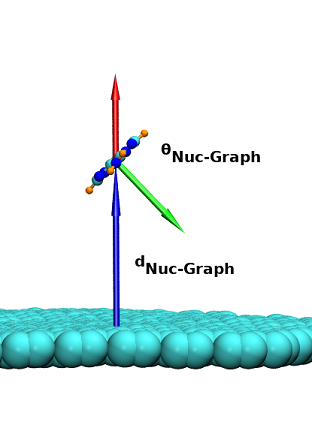
\includegraphics{Chapter1/Figures/cv.png}
        \caption[Representative illustration of the CVs used to study the evolution of the interactions between the nucleobases and the underlying graphene sheet]{Representative illustration of the CVs used to study the evolution of the interactions between the nucleobases and the underlying graphene sheet. Relative orientations are calculated as \textit{arccos(z-axis * Normal)}. d\textsubscript{Nuc-Graph} is evaluated as the difference between z-coordinates of COM of nucleobase and graphene sheet.}
    \end{figure}

    In Figure 3.9(a) we present the distribution corresponding to the distance between the COM of the nucleobase and the graphene sheet (d\textsubscript{Nuc-Graph}). We clearly observe the formation of a monolayer for all nucleobases expect guanine, highlighting the fact that nucleobases tend to interact preferentially with the graphene sheet. The average d\textsubscript{Nuc-Graph} distances for adenine, cytosine, thymine and uracil were found to be 3.44 (3.62) $\angstrom$, 3.56 (3.62) $\angstrom$, 3.56 (3.73) $\angstrom$ and 3.92 (4.61), respectively, in additive (Drude) simulations. For guanine, in the Drude simulations, the bases arranged themselves to form 5 distinct layers at distances 3.66 $\angstrom$, 6.77 $\angstrom$, 10.09 $\angstrom$, 13.45 $\angstrom$ and 16.78 $\angstrom$ from the graphene sheet, as shown in Figure 3.9(b). The average d\textsubscript{Nuc-Graph} distance for guanine from the additive simulation was 3.67 $\angstrom$. In Figure A.5 of the Appendix A, we we also present the distribution of the relative orientations of the nucleobase with respect to the graphene sheet. We observe that all the nucleobases lie flat on the graphene sheet or within the stacks formed in the guanine Drude simulations.
    \begin{figure}
        \centering
        \includegraphics[width=\textwidth]{Chapter1/Figures/FigureCOM.png}
        \caption[Distribution of d\textsubscript{Nuc-Graph} of nucleobases: adenine, guanine, cytosine, thymine and uracil, respectively. Snapshot from the simulation trajectory of guanine showing the $\pi$-stack formation]{ (a) Distribution of d\textsubscript{Nuc-Graph} of nucleobases: adenine, guanine, cytosine, thymine and uracil, respectively. Signatures of $\pi$-stacks formed by guanine nucleobases in Drude simulations are discernible from the plot. (b) Snapshot from the simulation trajectory of guanine showing the $\pi$-stack formation.}
    \end{figure}

    The results observed by us for the additive simulations are in agreement with the earlier reports by Saikia et al.,\supercite{saikia_hierarchical_2017, saikia_dynamics_2018} wherein cytosine and guanine were found to preferentially tile the surface of the graphene sheet. Thus, we note that for the additive simulations, the nucleobase - nucleobase interactions die out quickly, as the nucleobase - graphene sheet $\pi$-interactions become dominant. However, in the Drude simulations, we observe the formation of $\pi$-stacks and even hydrogen-bonded structures.
    \begin{figure}
        \centering
        \includegraphics[width=\textwidth]{Chapter1/Figures/dipole_new.png}
        \caption[Probability distribution of instantaneous dipole moments for the nucleobases: adenine, guanine, cytosine, thymine and uracil, respectively]{Probability distribution of instantaneous dipole moments for the nucleobases: adenine, guanine, cytosine, thymine and uracil, respectively. Dipole moments are reported in units of Debye.}
    \end{figure}
    
    In an attempt to understand the influence of molecular polarizability on non-covalent interactions, we analyzed the instantaneous dipole moments of the nucleobases over the length of the simulation trajectory from both the nucleobase only and nucleobase - graphene simulations. The probability distributions of the instantaneous dipole moments from both the additive and Drude FF simulations are presented in Figure 3.10. We observe that the dipole moments from the Drude simulations are shifted to larger values when compared to the additive simulations. The average dipole moments from the nucleobase - graphene additive (Drude) simulations for A, G, C, T and U were found to be 3.0 (4.0) D, 7.6 (9.4) D, 8.2 (12.1) D, 4.6 (7.9) D and 4.5 (6.3) D, respectively. We found that the distribution of dipole moments did not show a strong dependency on the formation of self-assembled structures in the simulations. It was observed that the distributions of instantaneous dipole moments obtained from freebase and nucleobase - graphene sheet simulations showed an appreciable overlap in both additive and Drude simulations. This was especially true for the purine nucleobases, where no influence of the graphene sheet was observed on the values of the instantaneous dipole moments. For the pyrimidine nucleobases, we find a slight shift in the average dipole moment value in the presence of the graphene sheet. For cytosine, the value increased from 11.9 D to 12.1 D, while for T the value decreased from 8.3 D to 7.8 D. We note that this may be due to the formation of strong hydrogen-bonding observed in thymine.

    Finally, we analyze the simulations for the formation of local hydrogen-bonded structures on the graphene sheet. Nucleobases are known to form hydrogen-bonded self-assemblies on two dimensional supports such as Au(111) and Ag(111).\supercite{ciesielski_self-assembly_2016} Formation of the hydrogen-bonded ordered structures for nucleobases on the graphite surface has been observed for adenine,\supercite{freund_structure_1997} guanine\supercite{heckl_two-dimensional_1991} and uracil.\supercite{sowerby_scanning_1997} The experimental studies using scanning tunnelling microscopy (STM) and low-energy electron diffraction (LEED) found that the nucleobases formed a close-packed network of hydrogen-bonded dimers. Stability of the hydrogen-bond stabilized dimer and higher ordered structures were evaluated as a function of the probability of occurrence. We employed a cut-off of >25\% occurrences to classify the hydrogen-bonded structures as significant. We did observe the formation of hydrogen-bonded structures in additive simulations; however, the probabilities of these dimeric structures were found to be <25\%.  We note that this observation is in accordance with the earlier reports by Saikia et al.,\supercite{saikia_hierarchical_2017,saikia_dynamics_2018} who observed a dispersive behaviour for guanine and cytosine on graphene surfaces at low concentrations. For Drude simulations, we observed the formation of hydrogen-bonded structures even at the low concentrations (0.25 M) studied by us. The structures were found to be predominantly dimeric in nature, with the probabilities of the formation of stable dimeric structures for adenine, guanine, cytosine, thymine and uracil being between 33.45\%-50.76\%, 28.67\%-75.21\%, 33.92\%-88.20\%, 29.24\%-69.29\% and 39.20\%-75.06\%, respectively. In Figure A.6 of Appendix A, we present the probability of the formation of dimer pairs as a heat map. We observed the formation of 15, 15, 21, 9 and 4 dimers in adenine, guanine, cytosine, thymine and uracil simulations, respectively. To ascertain the lifetime for the dimer pairs, we also evaluated the hydrogen bond auto-correlation function. The plots for the hydrogen bond auto-correlation function are presented in Figure 3.11. The average lifetimes of the dimer pairs obtained by fitting the auto-correlation function using a two-term exponent are tabulated in Table 3.7 for both the additive and Drude polarizable FF simulations. The average lifetimes are found to be 23.68 ps and 65.11 ps for the additive and Drude simulations, respectively.
    \begin{figure}
        \centering
        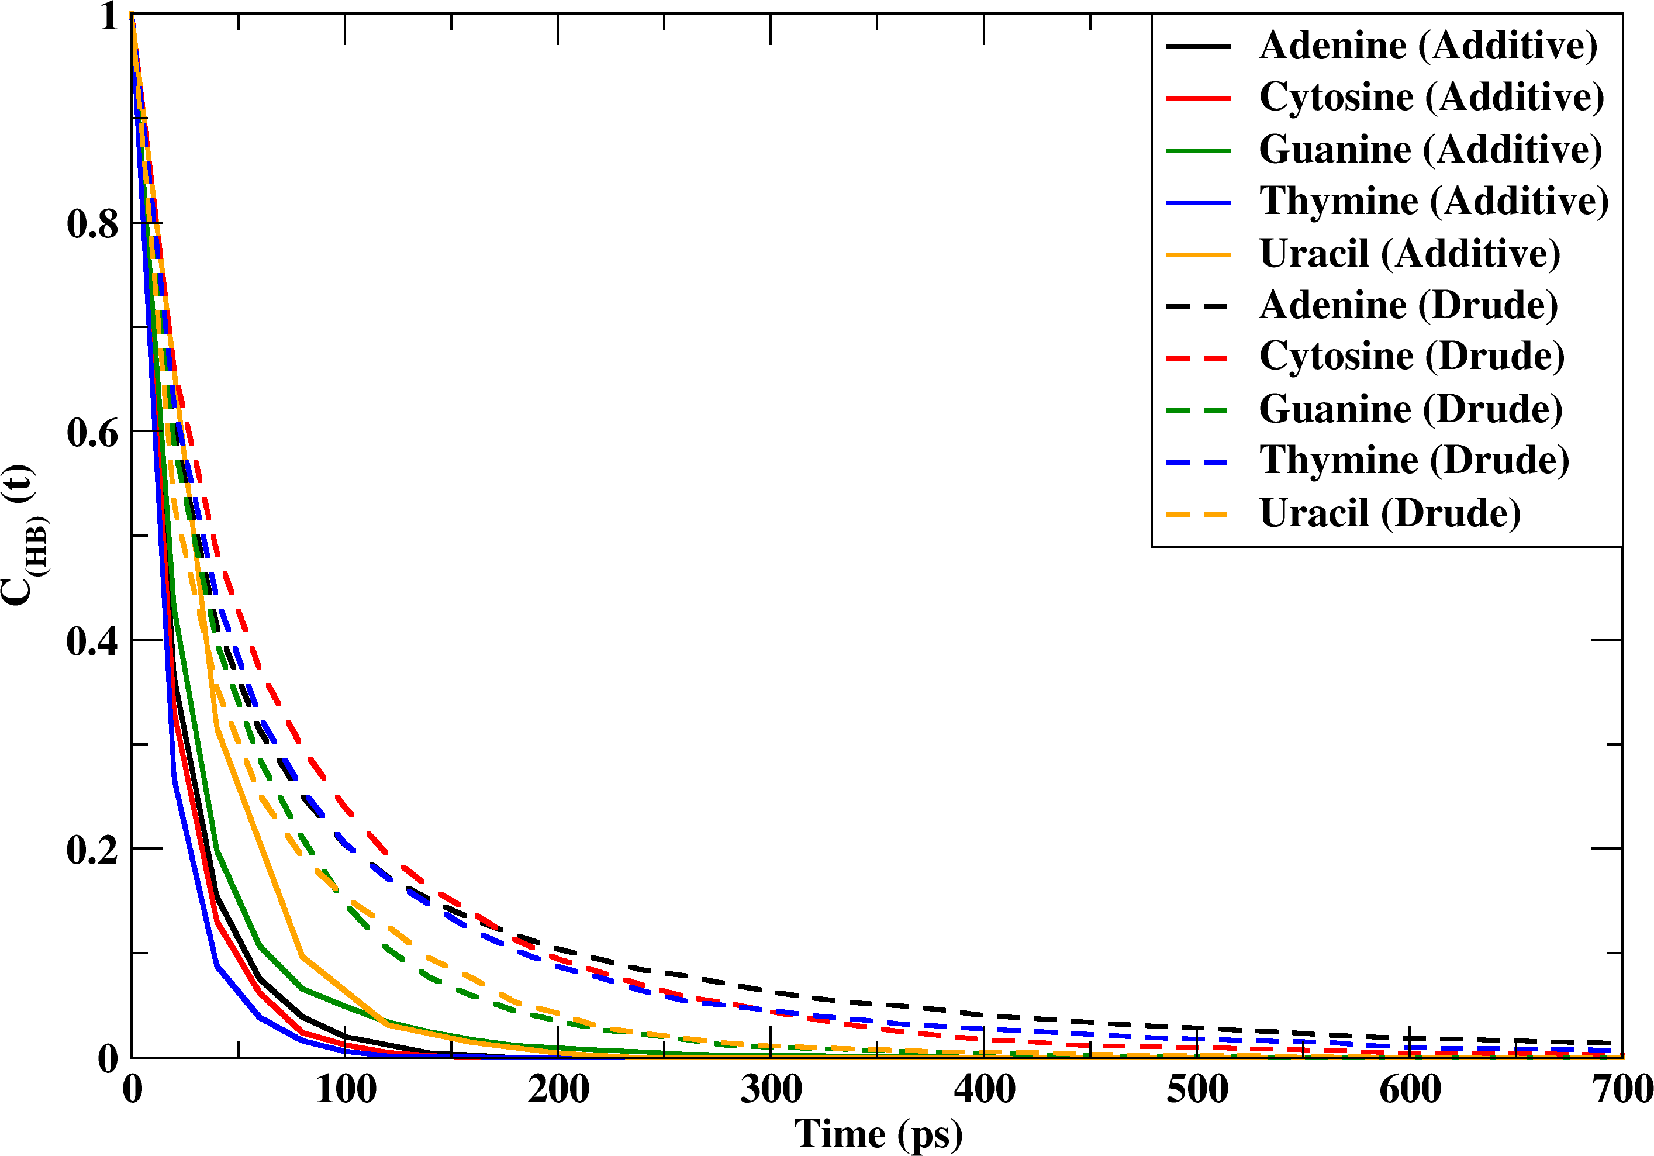
\includegraphics[width=\textwidth]{Chapter1/Figures/autocorrelation.png}
        \caption[Comparison of continuous hydrogen-bond auto-correlation function for the dimer pairs in the simulation systems]{Comparison of continuous hydrogen-bond auto-correlation function for the dimer pairs in the simulation systems.}
    \end{figure}
    \begin{table}
        \centering
        \caption[Average lifetimes of the hydrogen bonded dimers observed in the nucleobases for additive and Drude polarizable FF simulations.]{Average lifetimes of the hydrogen bonded dimers observed in the nucleobases for additive and Drude polarizable FF simulations. Lifetimes are calculated by fitting to a two term-exponential}
        \begin{tabular}{ccc}
            \toprule
            Nucleobase  &   $\tau$\textsubscript{additive}(ps)  &   $\tau$\textsubscript{Drude}(ps) \\ \midrule
            Adenine     &   21.73   &   79.86   \\
            Guanine     &   28.08   &   49.73   \\
            Cytosine    &   19.39   &   74.94   \\
            Thymine     &   14.49   &   71.88   \\
            Uracil      &   34.72   &   49.17   \\
            $\tau$\textsubscript{Average}   &   23.68   &   65.11   \\ \bottomrule
        \end{tabular}
    \end{table}
    \begin{figure}
        \centering
        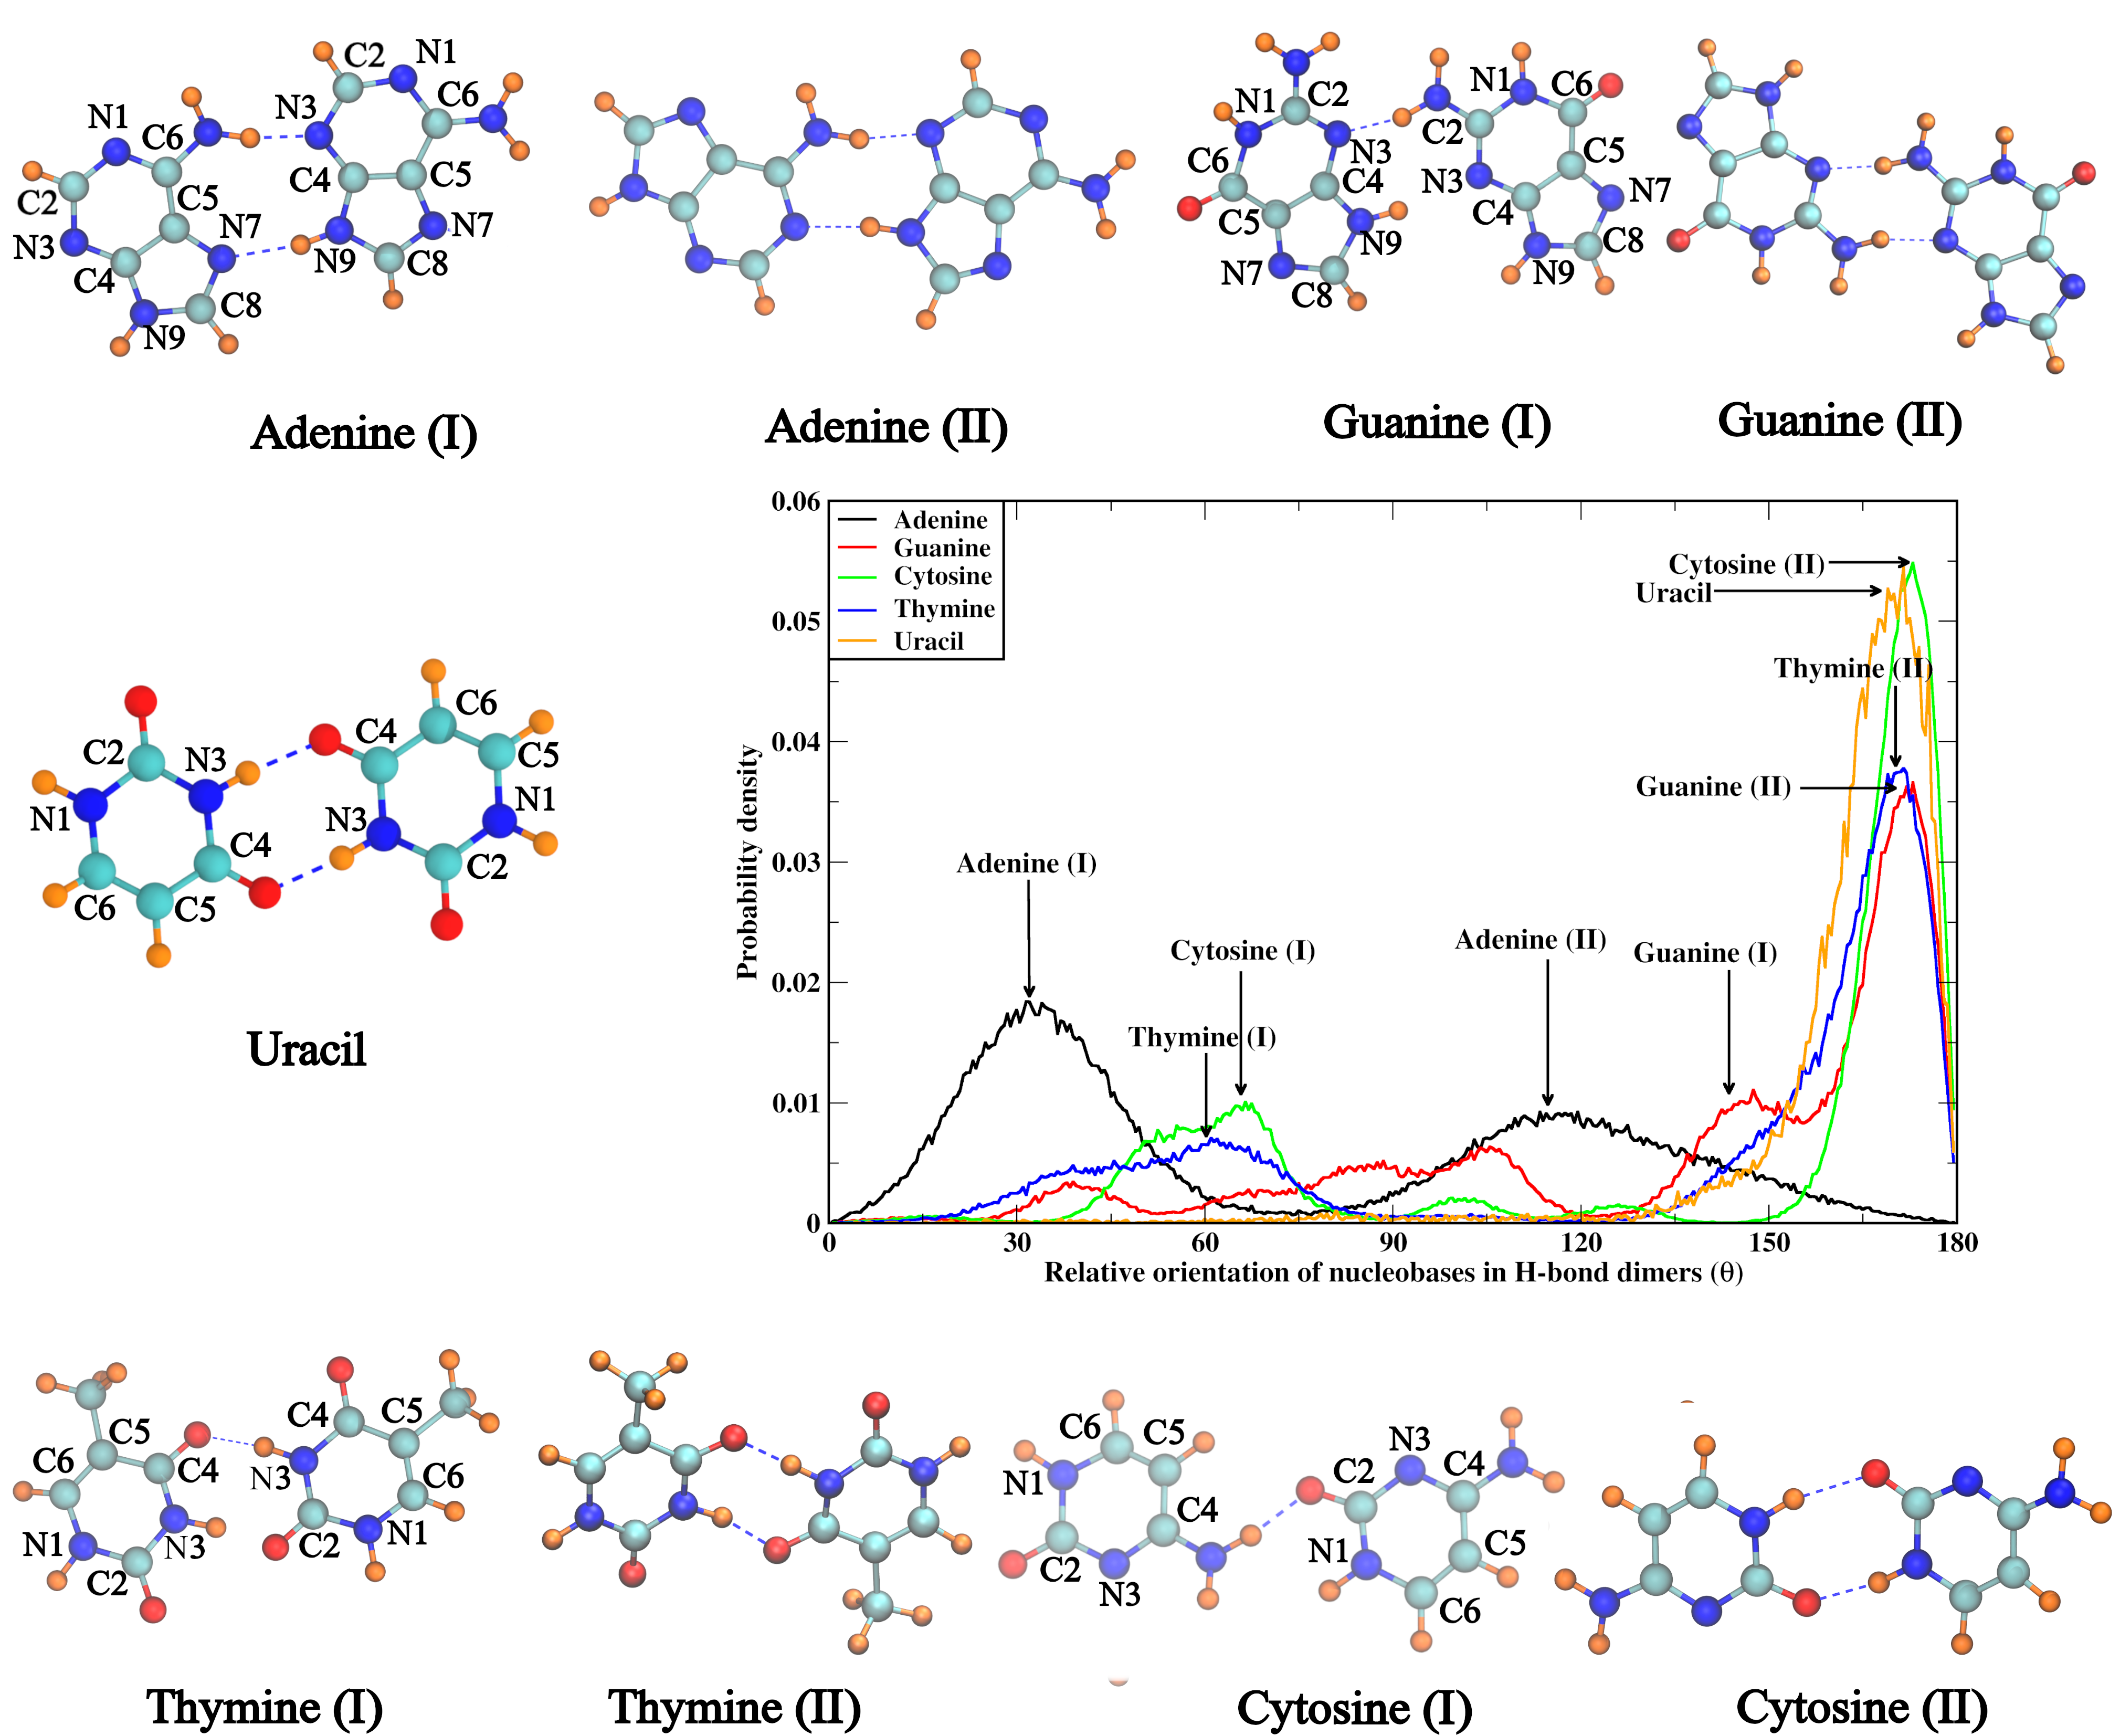
\includegraphics[width=\textwidth]{Chapter1/Figures/hbonds_full_mod_new1.png}
        \caption[Relative orientation of nucleobases in hydrogen-bonded dimers observed in homogeneous Drude FF simulations. Structures corresponding to the most significant hydrogen-bonded dimer pairs have also been presented]{Relative orientation of nucleobases in hydrogen-bonded dimers observed in homogeneous Drude FF simulations. Structures corresponding to the most significant hydrogen-bonded dimer pairs have also been presented. Carbon atoms are coloured green, nitrogen atoms are blue, oxygen atoms are red and hydrogen atoms are orange.}
    \end{figure}
    % \begin{figure}
    %     \centering
    %     \includegraphics[width=\textwidth]{Chapter1/Figures/adenine_network_compressed.png}
    %     \caption[ Representative image showing various hydrogen-bonded structures formed by Adenine on graphene sheet]{ Representative image showing various hydrogen-bonded structures formed by Adenine on graphene sheet}
    % \end{figure}
    \begin{table}
        \centering
        \caption[Prominent Hbonds between nucleobases in homogeneous nucleobase - graphene Drude polarizable FF simulations]{Hbond pairing among the nucleobases in homogeneous nucleobase - graphene Drude polarizable FF simulations.}
        \begin{tabular}{cccc}
            \toprule
            Structure   & Nucleobase 1  & Nucleobase 2  & Orientation (\degree)\\ \midrule
            Adenine(I)  & -NH$_2$       & N3            & 31.5\degree \\
                        & N7            & N9 \\ 
            Adenine(II) & -NH$_2$       & N3            & 113.5\degree \\
                        & N1            & N9 \\ 
            Guanine(I)  & -NH$_2$       & N3            & 145\degree \\
            Guanine(II) & -NH$_2$       & N3            & 173\degree \\ 
                        & N3            & -NH$_2$ \\ 
            Cytosine(I) & -NH$_2$       & C2(O)         & 67\degree \\ 
            Cytosine(II)& C2(O)         & N1            &   173\degree\\ 
                        & N1            & C2(O) \\ 
            Thymine(I)  &   C4(O)       &   N3          &   60\degree   \\
            Thymine(II) &   C4(O)       &   N3          &   173\degree  \\
                        &   N3          &   C4(O)   \\  
            Uracil      &   C4(O)       &   N3          &   173\degree  \\
                        &   N3          &   C4(O)   \\      \bottomrule
        \end{tabular}
    \end{table}

    \begin{figure}
        \centering
        \includegraphics{Chapter1/Figures/cytosine_figure1.png}
        \caption[Representative image showing the self-organised C1-D(2) ribbon-type higher-order structures formed by cytosine on the graphene sheet.]{Representative image showing the self-organised C1-D(2) ribbon-type higher-order structures formed by cytosine on the graphene sheet.}
    \end{figure}
    
    Upon analyzing the structural characteristics of the dimer pairs, we observed that the various dimeric assemblies formed amongst the nucleobases could be classified using the relative orientation of the bases in the dimer pairs. Hydrogen-Bonded dimer pairs were identified by enforcing a distance cut-off of 3.0 $\angstrom$ between the hydrogen-bond donor (D) and acceptor (A) atoms, and an angle cut-off of 20$\degree$ between the vectors lying along D-H and H-A bonds. In Figure 3.12, we present the relative orientation of the nucleobases in hydrogen-bonded dimer pairs. For adenine, we find the formation of two unique dimer pairs with a relative average orientation of 31.5$\degree$ [adenine(I)] and 113.5$\degree$ [adenine(II)]. The conformations corresponding to adenine(I) and adenine(II) are presented in Figure 3.12.  In both adenine(I) and adenine(II), we observe the formation of two hydrogen-bonds between the adenine nucleobases. The atoms involved in the formation of the hydrogen-bonds are listed in Table 3.8.  Besenbacher et al. used ab initio calculations to explore the various dimeric structures, which could be formed in adenine and cytosine monolayers deposited on the Au(111) surface.\supercite{kelly_understanding_2008, lukas_adenine_2009} The dimeric structures formed within the simulation cell for adenine, adenine(I) and adenine(II) are consistent with the structures A\textsubscript{1}A\textsubscript{5} and A\textsubscript{2}\={A}\textsubscript{5} reported by Besenbacher et al.\supercite{kelly_understanding_2008} using ab initio calculations and STM observations. In Figure A.7 of the Appendix A, we present representative snapshots of the self-assembly of adenine dimers on the graphene sheet. For guanine, cytosine and thymine, we find the formation of a dominant hydrogen-bonded dimer with a relative angle of 173$\degree$ when compared to adenine, wherein we observed two hydrogen-bonded dimers with similar occurrences.  In Figure 3.12, we also present the conformations corresponding to these dominant hydrogen-bonded dimers for guanine, cytosine and thymine. In contrast to the adenine hydrogen-bonded dimers for guanine, cytosine, thymine and uracil, we observe the formation of symmetric hydrogen-bonded dimers, with the same atoms being involved in the formation of hydrogen-bonds in the two nucleobases. For guanine(II), the hydrogen-bonds are formed between the amino (-NH\textsubscript{2}) group and the N3 nitrogen, for cytosine(II) the hydrogen-bonds are formed between the C2 carbonyl oxygen and the N1 nitrogen, for thymine(II) the hydrogen-bonds are formed between the C4 carbonyl oxygen and the N3 nitrogen, and for uracil the hydrogen-bonds are formed between the C4 carbonyl oxygen and the N3 nitrogen. The other hydrogen-bonded structures among guanine, cytosine and thymine (guanine(I), cytosine(I) and thymine(I)) were found for transient structures with only one hydrogen-bond between the nucleobases. It is interesting to note that the symmetric dimers found in guanine, cytosine, thymine and uracil have been observed in experimental assemblies.\supercite{kelly_understanding_2008, lukas_adenine_2009, sowerby_scanning_1997, otero_elementary_2008, spada_guanosine-based_2008, xu_probing_2007} The guanine dimer with hydrogen-bonds between the amino (-NH\textsubscript{2}) group and the N3 nitrogen has been observed to be an integral part of the G-ribbon B structure reported by Spada et al.,\supercite{spada_guanosine-based_2008} wherein the guanine nucleobases were self-assembled on a graphite support. The cytosine dimer structure, with hydrogen-bonds between the C2 carbonyl oxygen and the N1 nitrogen, has been observed to be a part of the C-1D(2) ribbon structure studied by Besenbacher et al.\supercite{otero_elementary_2008} for the cytosine assemblies on the Au(111) support. It was found that cytosine could assemble into multiple patterns on the Au(111) support by the formation of zigzag filaments and five- and six-membered rings. Central to all these self-assemblies was the formation of various dimeric conformations between the cytosine nucleobases, highlighting the importance of dimerization in the self-assembly.  In Figure 3.13, we present a snapshot from the Drude simulations, wherein we observed the self-assembly of the cytosine dimers to aggregate and form C-1D(2) ribbon-like structures observed by Besenbacher et al.\supercite{otero_elementary_2008} for the cytosine assemblies on the Au(111) support. Similar to the pattern formation in cytosine, Besenbacher et al. also studied the formation of supramolecular assemblies in thymine.\supercite{xu_probing_2007} The thymine dimers reported by us were observed in the island structures of thymine assemblies on the Au(111) support. Uracil dimers reported by us were observed in the herringbone structures of uracil assemblies on graphite and molybdenum disulphide surfaces.\supercite{sowerby_scanning_1997,sowerby_molecular_1998}

    \subsubsection{Heterogeneous nucleobase - graphene system}
    Nucleobases have the unique ability to form specific inter-molecular hydrogen-bonds, which leads to the formation of well-known Watson-Crick base pairs between adenine : thymine and guanine : cytosine. To explore the formation of such base pairs, we analyze two sets of heterogeneous systems, adenine with thymine and guanine with cytosine, to explore the spontaneous formation of hydrogen-bond stabilized base pairs over the graphene sheet. The simulation cell consisted of 15 nucleobases of purine (A/G) and pyrimidine (T/C) type, accounting for 30 nucleobases per cell. Heterogeneous simulations were performed at a concentration of 0.16 M. We restrict the analyses to only Drude polarizable FF simulations, wherein we observed significant aggregation and higher-order structures.
    \begin{figure}
        \centering
        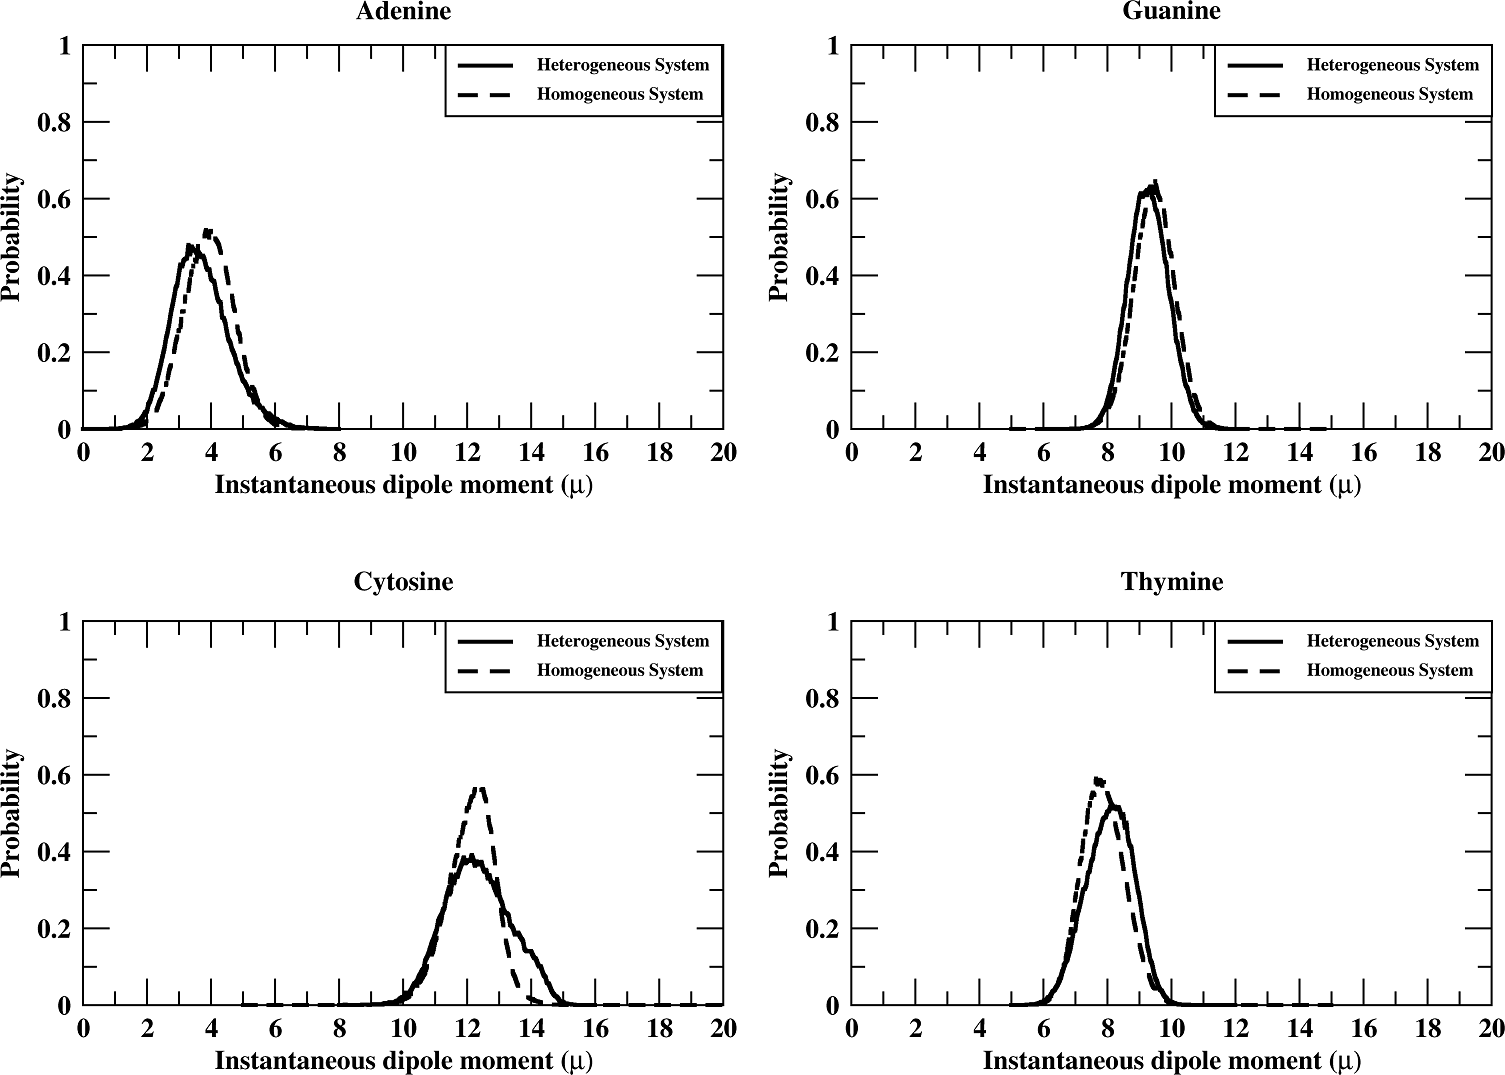
\includegraphics[width=\textwidth]{Chapter1/Figures/hetdipole.png}
        \caption[Probability distribution of Instantaneous dipole moments for nucleoobases; Adenine, Guanine, Cytosine, Thymine and Uracil respectively]{Probability distribution of Instantaneous dipole moments for nucleoobases; Adenine, Guanine, Cytosine, Thymine and Uracil respectively. Dipole moments are reported in units of Debye}
    \end{figure}
    We analysed the instantaneous dipole moments over the length of the trajectory for heterogeneous nucleobase - graphene simulations, and the results were compared with the values obtained from the homogeneous nucleobase - graphene simulations. The probability distributions of instantaneous dipole moments from both homogeneous and heterogeneous nucleobase - graphene simulations are presented in Figure 3.14. The average dipole moments from homogeneous and heterogeneous nucleobase - graphene simulations of the DNA nucleobases are presented in Table 3.9. The average dipole moments from the heterogeneous nucleobase - graphene (homogeneous) simulations for A, G, C and T were found to be 3.7 (4.0) D, 9.3 (9.4) D, 12.3 (12.1) D and 8.0 (7.9) D, respectively. The difference in dipole moments is also presented in Table 3.9. We observed that the dipole moments from heterogeneous simulations undergo shifts when compared to the homogeneous simulations. Dipole moments of purine nucleobases: adenine ($\Delta\mu$ = -0.3) and guanine ( $\Delta\mu$ = -0.1) were found to shift to lower values in comparison with the values from the homogeneous simulations. The dipole moments of cytosine ( $\Delta\mu$ = 0.2) and thymine ( $\Delta\mu$ = 0.1), being pyrimidine nucleobases, underwent shifts towards higher values in comparison with the homogeneous simulations. We note that our results are in line with the observations in base flipping.\supercite{lemkul_induced_2014} However, the magnitude of change in dipole moment is less compared to base flipping.
    \begin{table}
        \centering
        \caption[Instantaneous dipole moments of nucleobases from homogeneous and heterogeneous nucleobase - graphene simulations]{Instantaneous dipole moments of nucleobases from homogeneous and heterogeneous nucleobase - graphene simulations}
        \begin{tabular}{cccc}
            \toprule
            Nucleobase  &   Dipole moment ($\mu$)   &   Dipole moment ($\mu$)   & $\Delta\mu$\\
                        &   homogeneous             &   heterogeneous           &           \\  \midrule
            Adenine     &   4.0                     &   3.7                     &   -0.3    \\
            Guanine     &   9.4                     &   9.3                     &   -0.1    \\
            Cytosine    &   12.1                    &   12.3                    &   0.2     \\
            Thymine     &   7.9                     &   8.0                     &   0.1     \\  \bottomrule
        \end{tabular}
    \end{table}
    
    We next investigate the formation of hydrogen-bonded structures in the heterogeneous systems. Using the same distance and angle cut-offs to identify a hydrogen bond as discussed for the homogeneous system, we identify hydrogen-bonded dimer pairs in the heterogeneous system. We did not observe significant formation of hydrogen-bonded structures from the heterogeneous nucleobase - graphene sheet simulations using additive FF. We have presented the heat maps depicting the probabilities of the formation of various dimer pairs from the additive FF simulations in Figure A.8 of the Appendix A. For the Drude simulations we observed that in the heterogeneous system, the hydrogen bonds are only observed between purine and pyrimidine bases, i.e. between adenine and thymine or guanine and cytosine. We did not observe hydrogen bonds between purine bases or pyrimidine bases such as A : A, T : T, G : G or C : C. The probabilities of the formation of dimeric structures were between 52.62\%-83.71\% and 39.14\%-90.16\% for the adenine - thymine and guanine - cytosine pairs, respectively. We observed the formation of 10 dimers in the adenine - thymine and guanine - cytosine simulations, respectively. The probabilities of the formation of various heterogeneous nucleobase dimer pairs from the Drude polarizable FF simulations are presented as a heat map in Figure A.9 in Appendix A.
    \begin{figure}
        \centering
        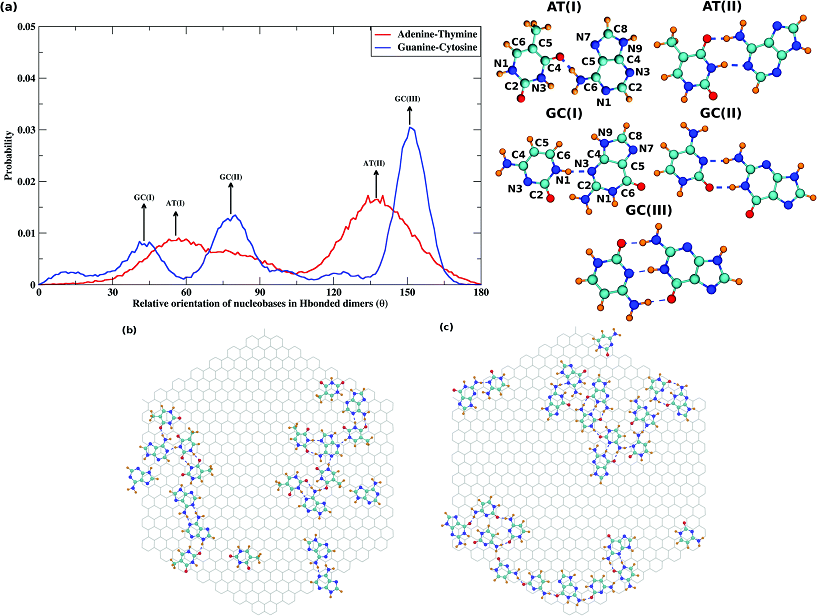
\includegraphics[width=\textwidth]{Chapter1/Figures/Figurelast.png}
        \caption[Relative orientation of nucleobases in the hydrogen-bonded dimers observed in heterogeneous Drude FF simulations. Structures corresponding to the most significant hydrogen-bonded dimer pairs have also been presented]{(a) Relative orientation of nucleobases in the hydrogen-bonded dimers observed in heterogeneous Drude FF simulations. Structures corresponding to the most significant hydrogen-bonded dimer pairs have also been presented. Carbon atoms are coloured green, nitrogen atoms are blue, oxygen atoms are red and hydrogen atoms are orange. Representative image showing higher-order structures in (b) A : T and (c) G : C simulations.}
    \end{figure}

    In Figure 3.15(a), we present the relative orientation of the nucleobases involved in hydrogen-bonded dimers. We use this analysis to identify the distinct interaction modes between the nucleobases. For adenine and thymine dimer pairs, we observe a bimodal distribution for the relative orientations centered at 31.5$\degree$ [AT(I)] and at 113.5$\degree$ [AT(II)]. The first peak [AT(I)] corresponds to the formation of a single hydrogen bond between A and T, which is also reflected by the broad distribution. The second peak (AT(II)) corresponds to the formation of the conventional Watson-Crick hydrogen-bonded structure, with two hydrogen bonds between A and T. The representative structures of the hydrogen-bonded dimers and the atoms involved in the hydrogen-bonds are presented in Fig. 3.14(a). The atoms involved in the formation of hydrogen-bonds are listed in Table 3.10. For guanine and cytosine dimer pairs, we observe three distinct peaks in the distribution for the relative orientations centered at 41$\degree$ [GC(I)], 80$\degree$ [GC(II)] and 151$\degree$ [GC(III)], respectively. The representative structures corresponding to these peaks are presented in Figure 3.15(a). We observe that these distributions correspond to the formation of a single hydrogen-bond [GC(I)], two hydrogen-bonds [GC(II)] and three hydrogen-bonds[GC(III)] between guanine and cytosine. GC(III) corresponds to the canonical Watson-Crick hydrogen-bonded structure. The atoms involved in the hydrogen-bonds are presented in Table 3.10.
    \begin{table}
        \centering
        \caption[hydrogen-bond pairing among the nucleobases in the heterogeneous nucleobase - graphene simulation]{hydrogen-bond pairing among the nucleobases in the heterogeneous nucleobase - graphene simulation}
        \begin{tabular}{cccc}
            \toprule
            Structure   &   Nucleobase I            &   Nucleobase II           &   Orientation     \\   \midrule
            AT(I)       &   -NH\textsubscript{2}    &   N3                      &   31.5$\degree$   \\
                        &   N7                      &   N9                                          \\
            AT(II)      &   -NH\textsubscript{2}    &   N3                      &   113.5$\degree$  \\
                        &   N1                      &   N9                                          \\  
            GC(I)       &   N1                      &   N3                      &   41$\degree$     \\
            GC(II)      &   N3                      &   -NH\textsubscript{2}    &   80$\degree$     \\
                        &   C2(O)                   &   N1                                          \\
            GC(III)     &   C2(O)                   &   -NH\textsubscript{2}    &   115$\degree$    \\
                        &   N3                      &   N1                                          \\
                        &   -NH\textsubscript{2}    &   C6(O)                                       \\  \bottomrule
        \end{tabular}
    \end{table}

    We also analysed if the dimeric structures aggregated within the simulation cell to form higher-order assemblies. The ability of the nucleobases to form single and multiple hydrogen-bonds in A : T and G : C pairs enables the formation of higher-ordered structures, instead of dimers dispersed over the graphene sheet. Using STM imaging, Besenbacher et al. observed the formation of ordered structures for A : T and G : C pairs co-adsorbed on the HOPG surface.\supercite{mamdouh_supramolecular_2006,xu_coadsorption_2006} From the heat maps presented in Figure A.9 of the Appendix A, we observe the occurrences of a nucleobase being hydrogen-bonded to more than one partner. In Figures 3.15(b) and (c), we present representative snapshots of higher-order structures observed by us in A : T and G : C simulations. We observe that the structures are stabilized by different combinations of hydrogen-bonds, and are in agreement with the experimental results.

    \section{Conclusions}
    In summary, the results from the present study show a qualitative and quantitative agreement with the previously reported results in the literature, while improving upon the parameters available in the literature to describe a polarizable graphene sheet. We show that the inclusion of polarizability affects the outcome of simulations for both free-standing nucleobases and nucleobase - graphene sheet systems. It is shown that polarizability plays a crucial role in determining the fate of non-covalent interactions within the simulation cell. The observance of $\pi$-$\pi$ stacking interactions in guanine is consistent with the experimental observation of a strong hydrophobic-driven assembly in guanine nucleobases\supercite{varghese_binding_2009} and poly-G single strands,\supercite{akca_competing_2011} an effect which is not captured by additive simulations. The polarizable simulations were also able to accurately capture the observed phenomenon of the formation of H-bond stabilized dimers,\supercite{kelly_understanding_2008,lukas_adenine_2009,otero_elementary_2008,spada_guanosine-based_2008,xu_probing_2007} in contrast to additive simulations where no H-bond formation was observed amongst the nucleobases. We were also able to study the spontaneous formation of ordered self-assemblies in adenine and cytosine nucleobase-graphene systems, which have not been observed in additive simulations. We also explored the formation and dynamics of ordered self-assemblies in heterogeneous nucleobase - graphene sheet simulations. The study sheds light on the relative strengths of nucleobase - graphene sheet interactions and nucleobase - nucleobase interactions, and how the subtle interplay between the various forces dictates the evolution of the system. The parameters for the polarizable graphene sheet would also enable the study of other interfacial phenomena at the graphene surface.
    \chapter[Capturing Concentration-Induced Aggregation of Nucleobases on a Graphene Surface through Polarizable Force Field Simulations]{Capturing Concentration-Induced Aggregation of Nucleobases on a Graphene Surface through Polarizable Force Field Simulations \protect\footnote[3]{This chapter has been published as \textbf{H., Hemanth}, Yadav, P. K. and Mallajosyula*, S.S.; Capturing Concentration Induced Aggregation of Nucleobases on Graphene Surface Through Polarizable Forcefield Simulations; {\textit{J. Phys. Chem. C}, 2022, \textbf{31}, 13122 - 13131}}}
\section{Introduction}
Controlled supramolecular assemblies formed by small molecules on two-dimensional (2D) supports have attracted significant attention in the scientific community.\supercite{goronzy_supramolecular_2018, moradi_two-dimensional_2017,quesne-turin_first-principles_2017} Noncovalent interactions such as hydrogen bonding, $\pi$-$\pi$ stacking, and electrostatic interactions play a fundamental role in stabilizing such supra-molecular assemblies.\supercite{subramani_self-assembly_2012} Here, nucleobases offer a viable pathway to the realization of both structured and amorphous self-assemblies due to the presence of multiple hydrogen bond donors and acceptors.\supercite{saravanan_surface_2018, saikia_hierarchical_2017, freund_structure_1997, heckl_two-dimensional_1991, saikia_dynamics_2018, kelly_understanding_2008, lukas_adenine_2009, wandlowski_structure_1996, otero_elementary_2008}. Chemical moieties with a nucleobase core act as starting blocks for rosette nanotubes\supercite{marsh_self-complementary_1996, fenniri_helical_2001} and other self-assemblies.\supercite{lafitte_quadruply_2006, park_highly_2005, sessler_novel_2003} Self-assemblies formed by nucleobases or their derivatives have found applications in bionanotechnology\supercite{laguerre_synthetic_2015, suri_role_2009, song_self-assembled_2011} and catalysis.\supercite{chhabra_electroless_2011, borzsonyi_water-soluble_2010} A fundamental understanding of the behavior of nucleobases at the solid-liquid interface is also crucial in understanding the evolution of life from simple chemical moieties.\supercite{cassidy_guanine-centric_2014, sowerby_role_1998}

Cytosine, one of the five natural nucleobases, can spontaneously self-assemble into higher-order structures over various solid-state supports such as Au(111),\supercite{kelly_understanding_2008, otero_elementary_2008} Cu(111)\supercite{tanaka_two-dimensional_1996} and highly oriented pyrolytic graphite (HOPG).\supercite{xu_directional_2021} Electroanalytical studies coupled with in situ STM imaging by Wandloski et al. showed that cytosine self-assemblies respond to an external voltage.\supercite{wandlowski_structure_1996} Otero et al. studied the formation of self-assembled networks in cytosine adsorbed over a Au(111) surface.\supercite{otero_elementary_2008} They observed the formation of geometries like five-/six-membered rings and filaments, which exist as a part of a more extensive self-assembled random network; 2D structures like graphene provide unique solid-state supports that are truly atomistically thin, as compared to the solid-state supports like Au(111) and Cu(111) surfaces. It is of interest to explore if graphene as a support can exhibit self-assembly properties akin to the metallic solid-state supports.

Molecular dynamics (MD) simulations provide a computational framework to gain insight into the atomistic interactions involved in the interfacial phenomenon. MD simulations have been used to study the self-assembly of nucleobases and other small molecules on solid-state supports like Au(111),\supercite{rapino_modeling_2005, maleki_molecular_2011, rosa_enthalpyentropy_2014} \textit{h}-BN,\supercite{ding_adsorption_2013, saikia_polarity-induced_2018} graphene,\supercite{saikia_hierarchical_2017, saikia_dynamics_2018} C\textsubscript{2}N,\supercite{mukhopadhyay_gauging_2018, mukhopadhyay_screening_2020} g-C\textsubscript{3}N\textsubscript{4},\supercite{mukhopadhyay_delicate_2020} and black-PN.\supercite{mukhopadhyay_design_2018}  However, it has been found that simulations using additive force fields (FF) do not capture the self-assembly behavior of nucleobases on 2D supports, rather the simulations capture a dispersive behavior for nucleobases adsorbed over the graphene sheet.\supercite{saikia_dynamics_2018} Tekin et al. reported that a modified Buckingham potential could capture the self-assembly of cytosine until hexamers in MD simulations.\supercite{manukyan_first_2015} However, specialized potentials, like the ones developed by Tekin et al., might not be immediately transferable to systems containing biomolecular entities. Having a FF that captures both the aggregation dynamics of nucleobases and is readily compatible with other components of the simulation system is desirable to ensure the continued applicability of MD simulations to such problems. We have recently shown that MD simulations based on the Drude polarizable FF could accurately capture higher-order structures in cytosine molecules adsorbed on a graphene sheet.\supercite{h_polarization_2021} In our work we established that inclusion of polarization captured the $\pi$-$\pi$ stacking as well as hydrogen-bonded network formation, while additive simulations only resulted in random dispersion of nucleobases on the 2D graphene support. We refer the reader to an earlier work for a detailed comparison between the additive and polarizable simulations.\supercite{h_polarization_2021} We showed that cytosine molecules adsorbed onto the graphene sheet self-assembled into C1-D(2) ribbon type structures previously observed by Kelly et al. via STM imaging and DFT calculations.\supercite{kelly_understanding_2008}

Self-assembly studies are generally hampered by the formation of solution aggregate structures as opposed to the desirable uniformly dispersed monolayer self-assembly on the underlying solid-state support.\supercite{lotito_approaches_2017} The balance between solution aggregation and solid-supported monolayer formation is generally dependent on the concentration of the solute. In the present study, we investigate the effect of concentration on the adsorption dynamics and self-assembly of nucleobases in the presence of graphene as a solid support. To this end, we study the dynamics of cytosine nucleobases dispersed on the graphene sheet at three different concentrations 0.25 M (21 nucleobases), 0.50 M (45 nucleobases), and 0.75 M (60 nucleobases). The study reveals the dependence of concentration and the interplay of intermolecular nonbonded interactions, hydrogen bonding, and $\pi$-$\pi$ interactions, controlling the formation of the observed structures.

\section{Computational Methodology}
Graphene sheets, with a radius of 21 $\angstrom$ and height of 2 $\angstrom$, were constructed using Inorganic Builder Toolkit available in VMD.\supercite{humphrey_vmd_1996} We used two graphene sheets separated by 55 $\angstrom$ to model the graphene surface. The molecular geometries of cytosine nucleobases were generated utilizing the topology information present in the Chemistry at Harvard Molecular Mechanics (CHARMM) additive nucleic acid FF\supercite{hart_optimization_2012, foloppe_all-atom_2000, mackerell_all-atom_2000} (CHARMM36) using the CHARMM program.\supercite{brooks_charmm_1983, brooks_charmm_2009} On the basis of the concentration, 21 nucleobases (0.25 M), 45 nucleobases (0.50 M), and 60 nucleobases (0.75 M) were added to the system. The nucleobases were initially arranged as an ordered matrix, with the interplanar distances set to 7 $\angstrom$ in all three dimensions, in an attempt to avoid biasing the system toward intermolecular $\pi$-stacking interactions. The layer closest to the graphene sheet in the cytosine matrix was placed at least 10 $\angstrom$ above the graphene sheet to avoid self-assembly bias. The nucleobase - graphene system was solvated using VMD to bring the system dimensions to (52 × 52 × 60) $\angstrom$\textsuperscript{3} The Drude particles were added to the final solvated systems using in-house scripts. In Figure 4.1, we present the representative structure depicting the system setup.

\begin{figure}
    \centering
    \includegraphics{Chapter2/Figures/Figure0.png}
    \caption[Representative structures of the initial system setup for various systems investigated in this paper]{Representative structures of the initial system setup for (a) 0.25M, (b) 0.50M, (c) 0.75M nucleobase - graphene, and (d) 0.60M freestanding nucleobase simulations. Carbon atoms are coloured green, nitrogen atoms are blue, oxygen atoms are red and hydrogen atoms are orange. Water molecules have been excluded from (a), (b) and (c) for clarity}
\end{figure}

The MD simulations were performed in the isobaric-isothermal (NPT) ensemble using the Nanoscale Molecular Dynamics (NAMD) simulation package.\supercite{phillips_scalable_2005} The Classical Drude polarizable FF was used to describe the bonded and nonbonded interactions of the nucleobases. Classical Drude polarizable parameters previously tested by us for studying graphene - nucleobase interactions\supercite{h_polarization_2021} were used to describe the bonded and nonbonded interactions of the graphene sheet. Water molecules were described by SWM4-NDP polarizable water model\supercite{lamoureux_polarizable_2006} with bond lengths and bond angles constrained via the SETTLE\supercite{miyamoto_settle_1992} algorithm. Particle Mesh Ewald (PME) summation\supercite{darden_particle_1993} was used to evaluate electrostatic interactions with a cutoff of 9.0 $\angstrom$. All simulations were performed at room temperature (298 K) with Langevin dynamics and a Nos\'{e}-Hoover Langevin piston applied to maintain the pressure at 1 atm. An additional dual thermostat was applied to maintain the Drude particles in an ice bath at 1 K.

The nucleobase - graphene systems were minimized for 60000 steps using conjugate-gradient (CG) minimization to remove unfavorable contacts. Minimized structures were equilibrated in an NPT ensemble for 1 ns. The central atom of the graphene sheet was constrained using a harmonic potential of 1.0 kcal (mol $\angstrom$)\textsuperscript{-2} to ensure that the sheets did not slide during the simulations. No additional constraints were applied, with the sheets allowed to ``breathe'' over the course of the simulations. The equations of motion were integrated using a time step of 1 fs. Production simulations were carried out for 750 ns for all the nucleobase - graphene systems, except for the 0.75 M system which was run for 600 ns. 

To estimate the influence of the graphene surface on the aggregation dynamics of cytosine nucleobases we also simulated cytosine nucleobases in water. A 0.60 M system of cytosine nucleobases in a water box of dimensions (50 × 50 × 50) $\angstrom$\textsuperscript{3} was generated using CHARMM and VMD. A total of 45 nucleobases were arranged in an ordered matrix, with interplanar distances set to 7 $\angstrom$ in all dimensions to prevent the system from biasing toward intermolecular $\pi$-stacking interactions. The Drude particles were added to the final solvated system using in-house scripts. A representative image showing the system setup is presented in Figure 4.1. The system was minimized for 60000 steps using CG minimization and subsequently equilibrated in an isobaric-isothermal ensemble for 1 ns. Production simulations were carried out for 500 ns. The same simulation parameters as described earlier were used for studying the cytosine nucleobase water simulation.

Plugins available in VMD were used to analyze hydrogen bonds and instantaneous dipole moment of the nucleobases. In-house analysis scripts were used for analyzing the formation of $\pi$-stacks, hydrogen-bonded networks, and the relative orientation of the nucleobases.

\section{Results and Discussions}
In our earlier study, we observed that at low concentrations (0.25 M) the cytosine nucleobases formed a well-dispersed monolayer on the graphene sheet. This was characterized by analyzing two collective variables: (1) projected distance between the center-of-mass (COM) of the nucleobase and graphene sheet (d\textsubscript{Nuc-Graph}) and (2) relative orientation of the nucleobase with respect to the graphene sheet ($\theta$\textsubscript{Nuc-Graph}). In Figure 4.2, we illustrate the collective variables employed to track the interaction of nucleobases with the underlying graphene sheet.
In Figure B.1 of the Appendix B, we present the time series corresponding to d\textsubscript{Nuc-Graph} obtained from the 0.25, 0.50, and 0.75 M simulations. We observe that fluctuations in the d\textsubscript{Nuc-Graph} time series cease beyond 250 ns for the 0.25 and 0.50 M simulations, indicative of the systems reaching an equilibrium. For the 0.75 M simulations, the simulations are deemed convergent after first 100 ns, wherein the fluctuations in the d\textsubscript{Nuc-Graph} time series cease, denoting the equilibrium state.  In the remainder of the chapter, the last 500 ns of the simulation trajectories are used for analysis. In Figure B.2 of the Appendix B, we present the probability distribution corresponding to d\textsubscript{Nuc-Graph} evaluated for two blocks of the simulation trajectory, 250-500 ns and 500-750 ns, for the 0.25 and 0.50 M simulations. For the 0.75 M simulation, we present the probability distribution for blocks corresponding to 100-350 ns and 350-600 ns. We observe significant overlap between the distributions.
\begin{figure}
    \centering
    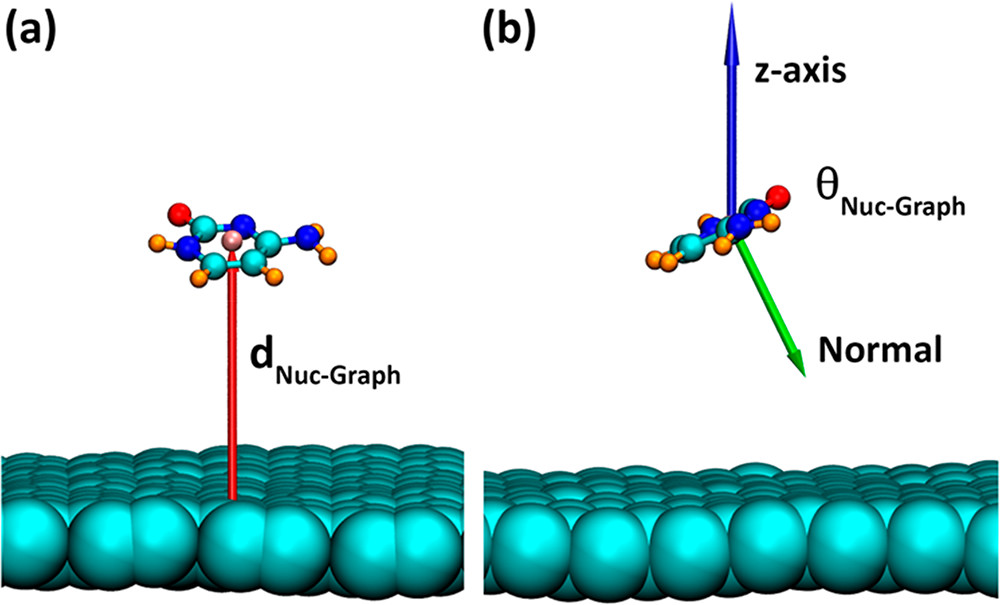
\includegraphics{Chapter2/Figures/Figure1.png}
    \caption[Representative illustration of collective variables used to study the evolution of nucleobase - graphene simulations]{Representative illustration of collective variables used to study the evolution of nucleobase - graphene simulations. (a) d\textsubscript{Nuc-Graph} and (b) $\theta$\textsubscript{Nuc-Graph}. d\textsubscript{Nuc-Graph} is calculated as the difference between the z-coordinates of the COM of nucleobase and top layer of the graphene sheet. $\theta$\textsubscript{Nuc-Graph} is calculated as \textit{arccos(Normal.z-axis)}.}
\end{figure}

\begin{figure}
    \centering
    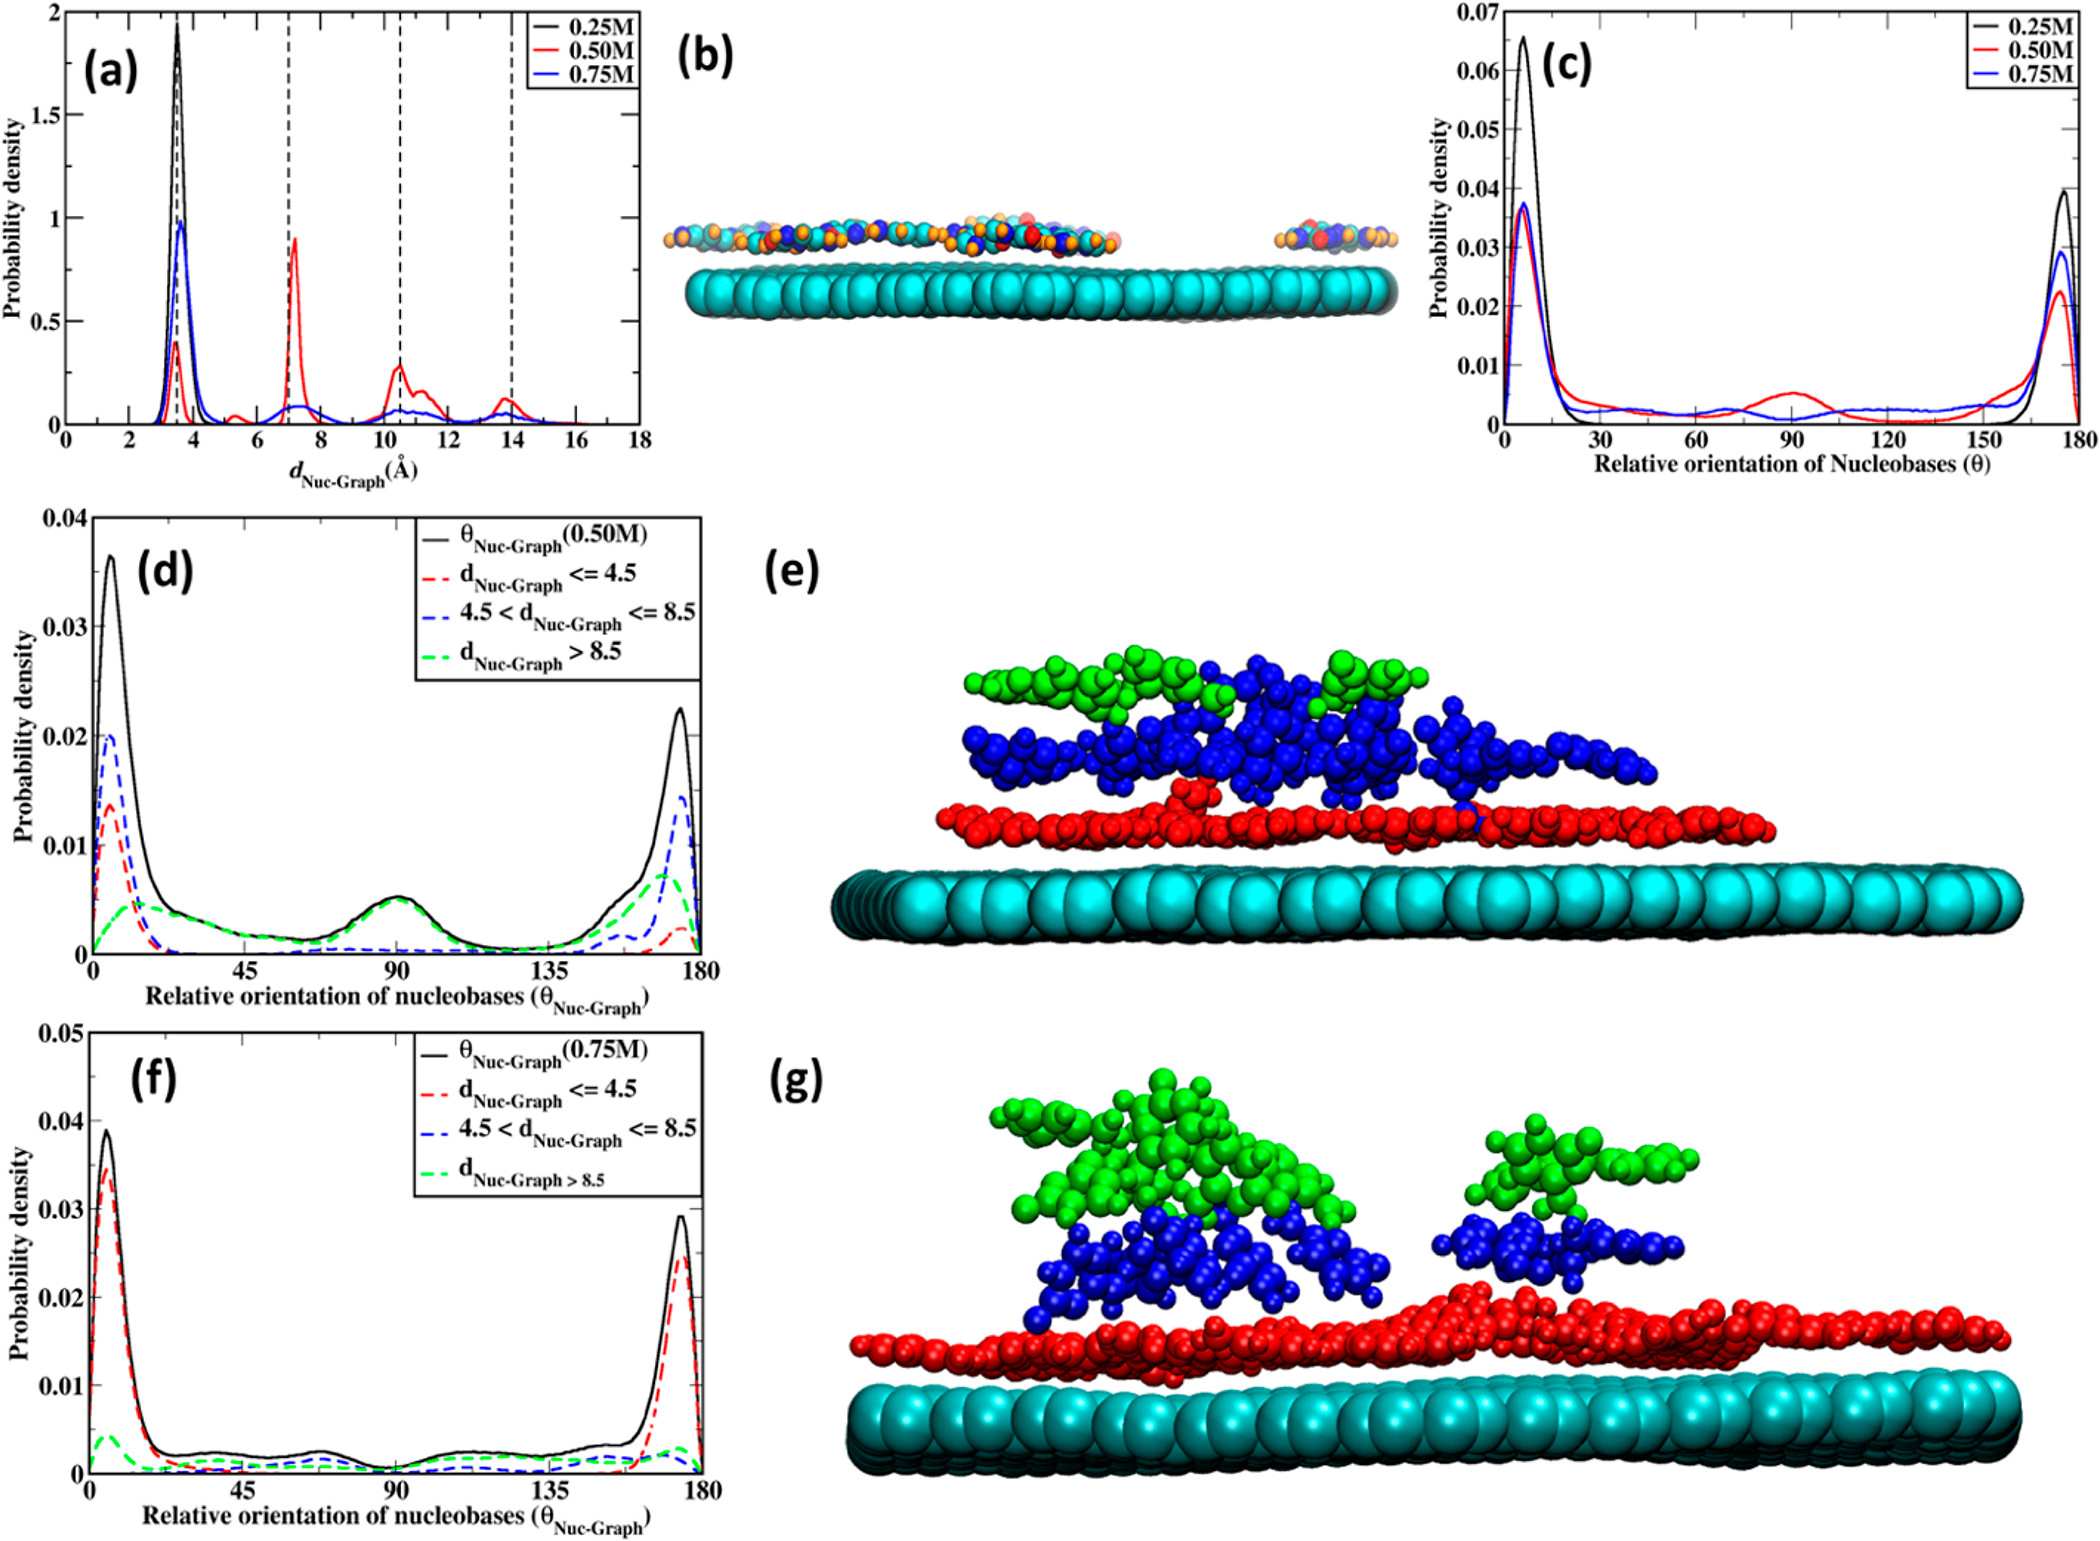
\includegraphics[width=\textwidth]{Chapter2/Figures/Figure2.png}
    \caption[Probability distribution of d\textsubscript{Nuc-Graph} and $\theta$\textsubscript{Nuc-Graph} for cytosine nucleobases at 0.25, 0.50, and 0.75 M, respectively. Representative structures corresponding to identified features are also presented]{Probability distribution of (a) d\textsubscript{Nuc-Graph} for cytosine nucleobases at 0.25, 0.50, and 0.75 M, respectively. (b) Representative image of the 0.25 M simulations, (c) Probability distribution of $\theta$\textsubscript{Nuc-Graph} for cytosine nucleobases at 0.25, 0.50, and 0.75 M, respectively. (d) $\theta$\textsubscript{Nuc-Graph} distribution as a function of d\textsubscript{Nuc-Graph} distance for 0.50 M simulations. (e) Representative image of the 0.50 M simulations, nucleobases in regions (i) (d\textsubscript{Nuc-Graph} < 4.5 $\angstrom$), (ii) (4.5 $\angstrom$ < d\textsubscript{Nuc-Graph} < 8.5 $\angstrom$), and (iii) (d\textsubscript{Nuc-Graph} > 8.5 $\angstrom$) are presented in red, blue, and green, respectively. (f) $\theta$\textsubscript{Nuc-Graph} distribution as a function of d\textsubscript{Nuc-Graph} distance for 0.75 M simulations. (g) Representative image of the 0.75 M simulations; color coding is similar to the representative image for 0.50 M simulations. Distances are presented in $\angstrom$ and orientations are presented in degrees (deg).}
\end{figure}
In Figure 4.3(a), we present the probability distribution corresponding to d\textsubscript{Nuc-Graph} for all the systems. For the 0.25 M simulations, we observe a single peak in the d\textsubscript{Nuc-Graph} distribution at a distance of 3.5 $\angstrom$ that is indicative of the formation of a monolayer of nucleobases on the graphene sheet [Figure 4.3(a)]. In Figure 4.3(b), we present a representative snapshot of the arrangement of the nucleobases on the graphene sheet from the 0.25 M simulations. In Figure 4.3(c), we present the probability distribution corresponding to $\theta$\textsubscript{Nuc-Graph} for all the systems. For the 0.25 M simulations, we observe that the formation of this monolayer is driven by the $\pi$-$\pi$ interactions between the nucleobase and the underlying graphene sheet. This observation is consistent with our earlier studies\supercite{h_polarization_2021} and the results previously reported by Saikia et al., where cytosine nucleobases were found to tile the surface of the graphene sheet.\supercite{saikia_dynamics_2018} The fact that the nucleobases lie flat on the graphene sheet is also corroborated by the $\theta$\textsubscript{Nuc-Graph} bimodal distribution for 0.25 M simulations with 175$\degree$ < $\theta$\textsubscript{Nuc-Graph} < 5$\degree$ [Figure 4.3(c)]. For 0.50 M simulations, we observe multiple peaks in the d\textsubscript{Nuc-Graph} distribution at around 3.5, 7.0, 10.5, and 14.0 $\angstrom$ [Figure 4.3(a)]. The peaks at 3.5 and 7.0 $\angstrom$ appear as sharp distributions, while the peaks at 10.5 and 14.0 $\angstrom$ appear as broad distributions. Analyzing the molecular interactions giving rise to these distributions, we observe that the peaks at 3.5 and 7.0 $\angstrom$ correspond to the formation of a monolayer assembly of the cytosine nucleobases. This is corroborated by analyzing the $\theta$\textsubscript{Nuc-Graph} distribution relative to the d\textsubscript{Nuc-Graph} distances presented in Figure 4.3(d). The $\theta$\textsubscript{Nuc-Graph} distribution is analyzed for three regions: (i) d\textsubscript{Nuc-Graph} < 4.5 $\angstrom$, (ii) 4.5 $\angstrom$ < d\textsubscript{Nuc-Graph} < 8.5 $\angstrom$, and (iii) d\textsubscript{Nuc-Graph} > 8.5 $\angstrom$. Regions (i) and (ii) correspond to the peaks at 3.5 and 7.0 $\angstrom$, while region (iii) corresponds to the broad distributions around 10.5 and 14.0 $\angstrom$. For both regions (i) and (ii), we observe a bimodal $\theta$\textsubscript{Nuc-Graph} distribution with 175$\degree$ < $\theta$\textsubscript{Nuc-Graph} < 5$\degree$, indicating that in both the distributions the nucleobases lie flat relative to the underlying graphene sheet. Thus, the monolayer at 3.5 $\angstrom$ is stabilized by $\pi$-$\pi$ interactions between the nucleobase and the underlying graphene sheet, while the monolayer at 7.0 $\angstrom$ is stabilized by $\pi$-$\pi$ interactions between the cytosine nucleobases in the first monolayer and the second monolayer. For region (iii), corresponding to nucleobases beyond 8.5 $\angstrom$, we observe a continuous distribution for $\theta$\textsubscript{Nuc-Graph} as opposed to the bimodal distribution observed for regions (i) and (ii). Both d\textsubscript{Nuc-Graph} and $\theta$\textsubscript{Nuc-Graph} indicate a disruption of the $\pi$-stacked monolayer structure beyond 8.5 $\angstrom$. This is due to nucleobase - nucleobase aggregation that is stabilized via intermolecular hydrogen bonding and $\pi$-$\pi$ interactions. In Figure 4.3(e), we present a representative snapshot from the 0.50 M simulation illustrating the arrangement of the nucleobases in the three regions as defined by the d\textsubscript{Nuc-Graph} distribution. Upon increasing the concentration to 0.75 M, we observe the formation of three distinct peaks in the d\textsubscript{Nuc-Graph} distribution, centered at 3.5, 7.0, and 10.5 $\angstrom$ [Figure 4.3(a)]. It is observed that the peak at 3.5 $\angstrom$ has a sharp feature, while the peaks at 7.0 and 10.5 $\angstrom$ appear as broad distributions. We analyze the $\theta$\textsubscript{Nuc-Graph} distribution for three regions: (i) d\textsubscript{Nuc-Graph} $\leq$ 4.5 $\angstrom$, (ii) 4.5 < d\textsubscript{Nuc-Graph} $\leq$ 8.5 $\angstrom$, and (iii) d\textsubscript{Nuc-Graph} > 8.5 $\angstrom$. The resulting distributions are presented in Figure 4.3(f). Nucleobases lying in the region d\textsubscript{Nuc-Graph} $\leq$ 4.5 $\angstrom$ lie flat on the graphene sheet, which is corroborated by the bimodal distribution of $\theta$\textsubscript{Nuc-Graph} with peaks centered at < $\theta$\textsubscript{Nuc-Graph} = 175$\degree$ and $\theta$\textsubscript{Nuc-Graph} = 5$\degree$. Thus, the nucleobases closest to the graphene sheet form a monolayer assembly stabilized by $\pi$-$\pi$ interactions between the nucleobases and underlying graphene sheet. For nucleobases lying in regions (ii) and (iii), we observe that $\theta$\textsubscript{Nuc-Graph} adopts a broad distribution, indicative of the formation of nucleobase aggregates, which are stabilized by intermolecular hydrogen bonding and $\pi$-$\pi$ interactions.
\begin{figure}
    \centering
    \includegraphics[width=\textwidth]{Chapter2/Figures/Figure3.png}
    \caption[Probability distributions of anngle between the normal ($\phi$) of the nucleobases involved $\pi$-stacks and hydrogen-bonded dimers. Representative structures corresponding to identified features are also presented.]{(a) Representative image from the 0.60 M nucleobase simulations. Hydrogen bonds are illustrated by dotted lines. (b) Probability distribution of the angle between the normal ($\phi$) of the nucleobases involved in $\pi$-stacks. Representative images illustrating the side-view and top-view of the antiparallel and parallel arrangement of the $\pi$-stacks corresponding to $\phi$ values of 42 and 138$\degree$. (c) Probability distribution of the angle between the normal ($\phi$) of the nucleobases involved in hydrogen-bonded dimers. Representative images illustrating the arrangement of the nucleobases corresponding to the peaks in the distribution.}
\end{figure}

\begin{figure}
    \centering
    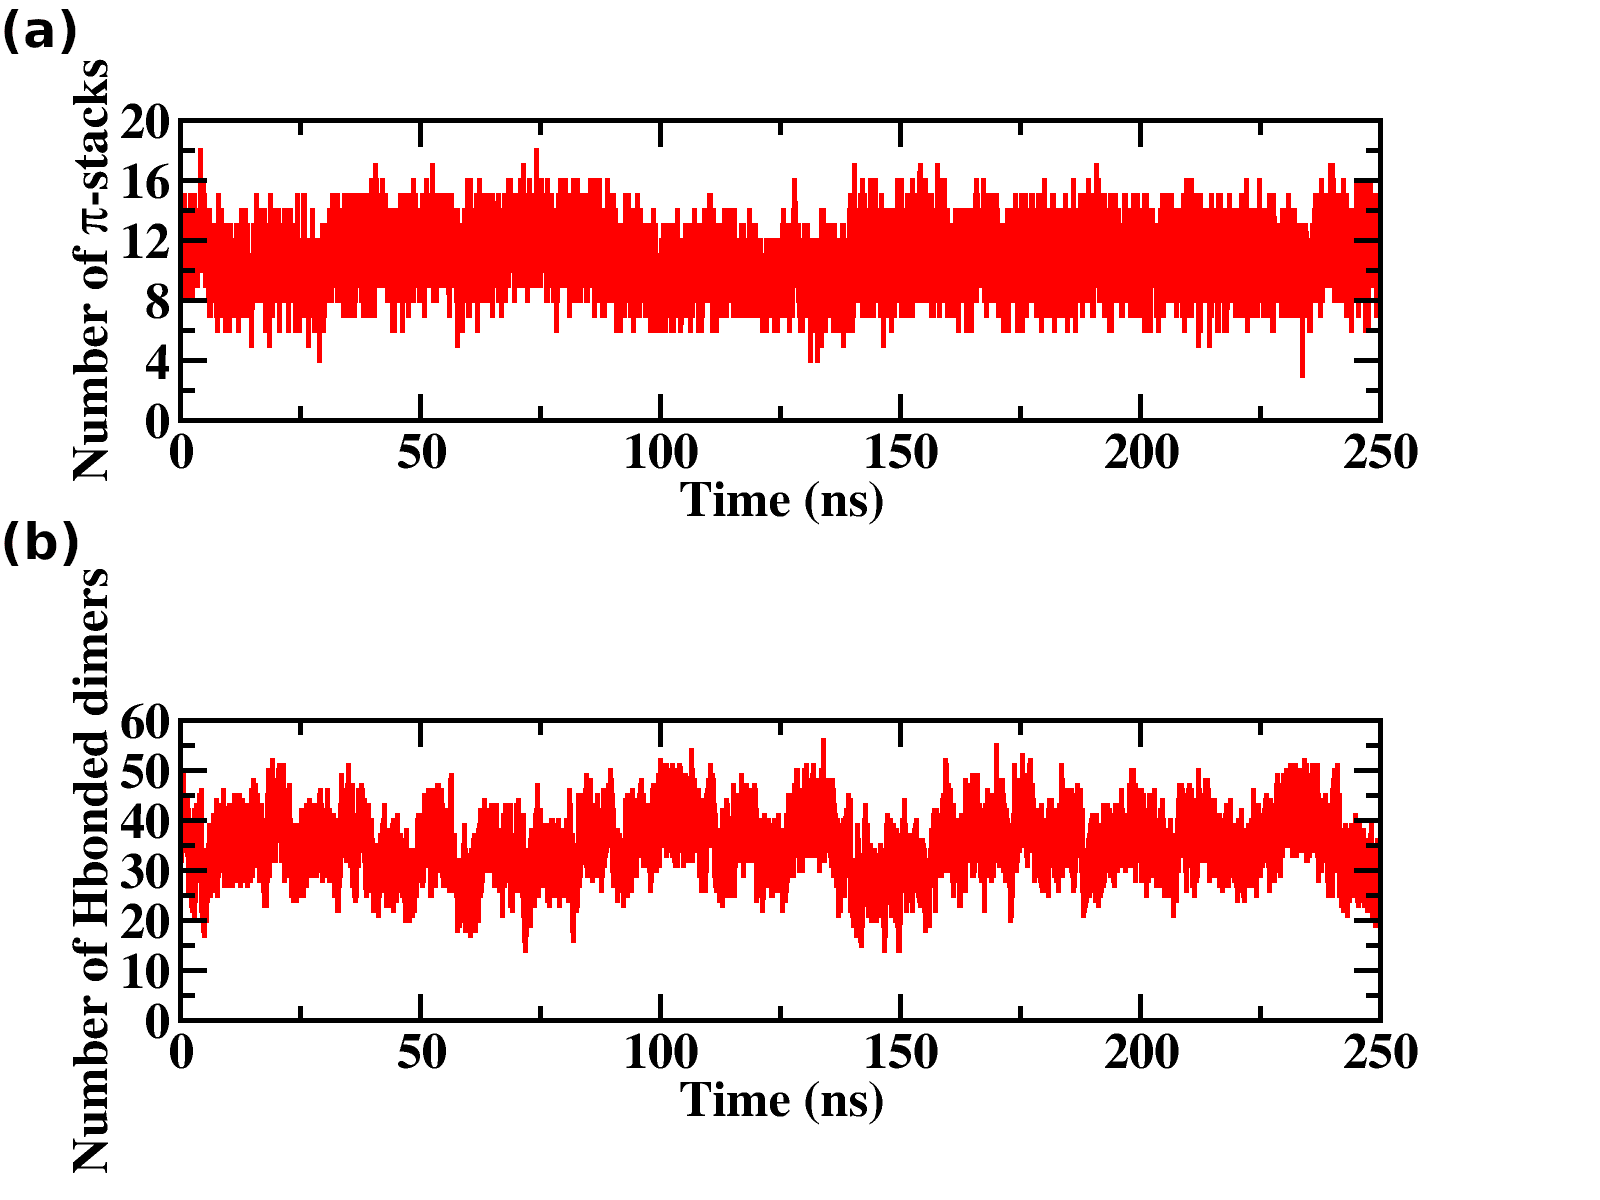
\includegraphics[width=\textwidth]{Chapter2/Figures/B3_port.png}
    \caption[Time series plots for number of $\pi$-stacks and hydrogen - bonded dimers in 0.60M simulations]{Time series plots for number of (a) $\pi$-stacks and (b) hydrogen - bonded dimers in 0.60M simulations.}    
\end{figure}

To comment on the aggregate structures, we analyze the solution structures obtained from the 0.60 M nucleobase-only simulations. In Figure 4.4(a), we present a representative snapshot obtained from the nucleobase only simulations. We observe aggregate formations which are stabilized by $\pi$-$\pi$ interactions and intermolecular hydrogen bonding. To quantify the $\pi$-stacked and hydrogen-bonded structures, we used a geometric criterion. $\pi$-stacked structures were identified by enforcing a distance cut off of 4.0 $\angstrom$ between the center of mass (d\textsubscript{COM-COM}) of the two nucleobases. Additionally, the angle between the normal ($\phi$) of the nucleobases involved in the $\pi$-stack was analyzed to identify the nature of the $\pi$-stacking.  For face-to-face stacking, the $\phi$ angle was considered to be less than 45$\degree$ or greater than 135$\degree$. All hydrogen-bonded dimers were identified by enforcing a distance cutoff of 3.0 $\angstrom$ between the hydrogen-bond donor (D) and acceptor (A), and an angle cutoff of 20$\degree$ between the vectors directed through D-H and D-A bonds. In Figure 4.5, we present the time series corresponding to the number of $\pi$-stacks and hydrogen-bonded dimers identified. We observe that on an average there are 10 $\pi$-stacks and 34 hydrogen-bonded dimer pairs among the cytosine nucleobases. This is indicative of aggregated structures. In Figure 4.4(b), we present the probability distribution corresponding to $\phi$ for all the identified $\pi$-stacked nucleobases. We observe a bimodal distribution, with peaks centered at 42 and 138$\degree$. This is indicative of a slipped-stacked arrangement of the nucleobases. In Figure 4.4(b), we present representative structures to illustrate the two $\pi$-stacked conformations. The 42 and 138$\degree$ stacked conformations correspond to the antiparallel and parallel arrangement of nucleobases with respect to each other as illustrated by the top view of the conformations in Figure 4.4(b). The average d\textsubscript{COM-COM} distance between the nucleobases forming the $\pi$-stacks was found to be 3.8 $\angstrom$. This value lies between the d\textsubscript{COM-COM} distances obtained for cytosine - cytosine $\pi$-stacked geometries from experimental X-ray structures (4.2 $\angstrom$) and theoretical (3.4 $\angstrom$) calculations.\supercite{mignon_influence_2005} We next analyze the relative orientation of the nucleobases in the hydrogen-bonded dimer pairs by calculating the angle between the normal of the nucleobases in the identified hydrogen-bonded dimer pair ($\phi$). The same is presented in Figure 4.4(c). We observe a very wide distribution with broad peaks centered at 43, 92, and 119$\degree$. We identify these peaks as Cyt(I), Cyt(II), and Cyt(III). In Figure 4.4(c) we present the representative structures corresponding to these peaks. For all the conformations we observe only a single hydrogen-bond between the nucleobases. For Cyt(I), Cyt(II), and Cyt(III) we observe the hydrogen-bonds between -NH\textsubscript{2} and N3, -NH\textsubscript{2} and O2, and -NH\textsubscript{2} and -NH\textsubscript{2} atoms, respectively.
\begin{figure}
    \centering
    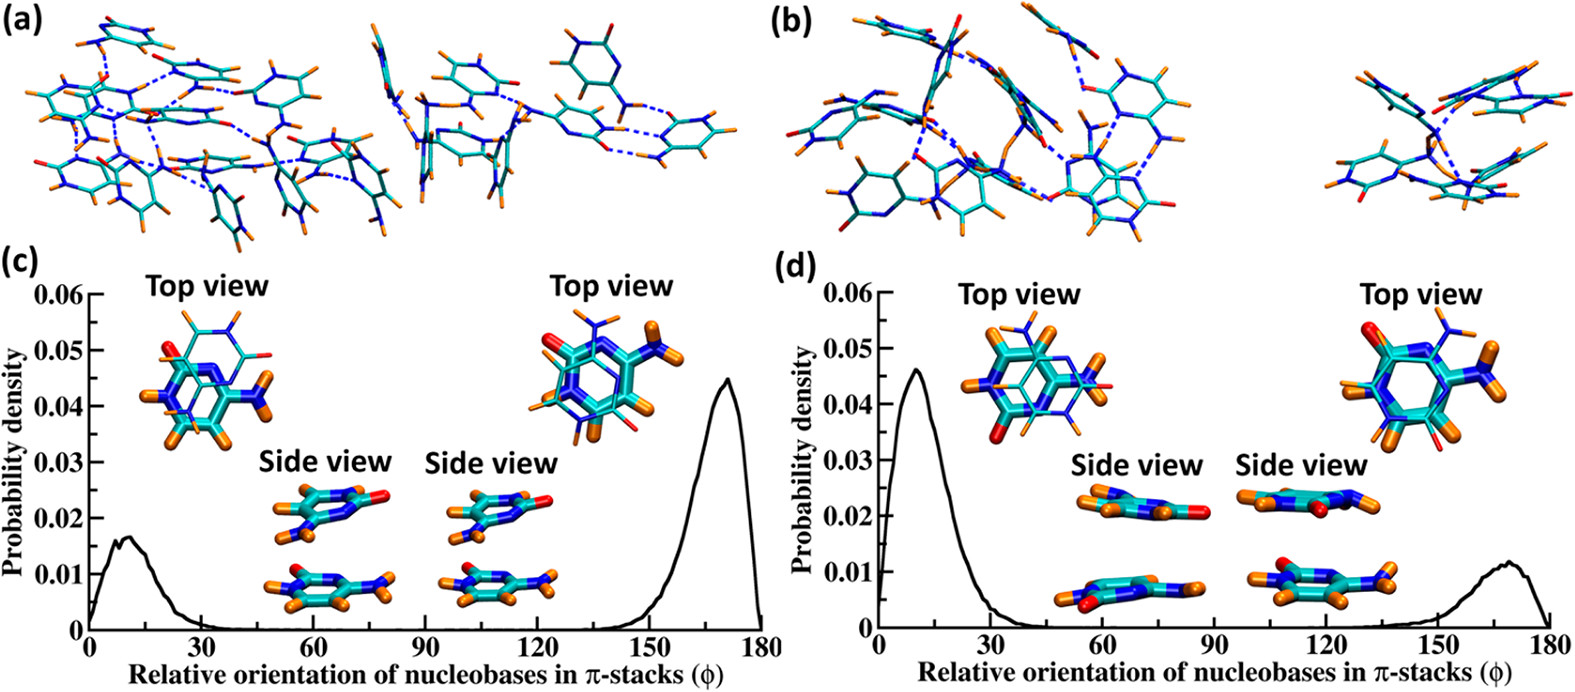
\includegraphics{Chapter2/Figures/Figure4.png}
    \caption[Representative structures depicting various aggregates formed in 0.50 and 0.75M simulations are presented. Probability distribution of the angle between the normal of the nucleobases ($\phi$) in the $\pi$-stacks are also presented]{Representative image from (a) 0.50 M and (b) 0.75 M simulation depicting the formation of aggregates. Probability distribution of the angle between the normal of the nucleobases ($\phi$) in the $\pi$-stacks from (c) 0.50 M and (d) 0.75 M simulations. Top and side views of the representative structures corresponding to the observed peaks are also presented.}
\end{figure}

On the basis of the analysis of the aggregate structures in solution we analyze the aggregate structures observed in the 0.50 and 0.75 M nucleobase - graphene simulations. We first analyze the formation of $\pi$-stacks before analyzing the formation of hydrogen-bonded structures. From Figure 4.2(d) and Figure 4.2(f), we observe that aggregate structures stabilized by $\pi$-$\pi$ interactions between the nucleobases are observed in regions (ii) 4.5 $\angstrom$ < d\textsubscript{Nuc-Graph} < 8.5 $\angstrom$ and (iii) d\textsubscript{Nuc-Graph} > 8.5 $\angstrom$. This is reflected in the $\theta$\textsubscript{Nuc-Graph} distribution. While the $\theta$\textsubscript{Nuc-Graph} exhibits a bimodal distribution for region (i) d\textsubscript{Nuc-Graph} $\leq$ 4.5 $\angstrom$, for regions (ii) and (iii) we observe a broad distribution spanning 0 - 180$\degree$ for both the 0.50 and 0.75 M simulations. The nucleobases in region (i) are stabilized by the $\pi$-$\pi$ interactions with the underlying graphene sheet, while in regions (ii) and (iii), they are stabilized by $\pi$-$\pi$ interactions among the nucleobases. The $\pi$-stacks are identified using the same geometric criterion of a distance cut off of 4.0 $\angstrom$ between the center of mass (d\textsubscript{COM-COM}) of the two nucleobases as described earlier. In Figures 4.6(a) and 4.6(b), we present the representative structures of the aggregates formed in regions (ii) and (iii). To identify the orientation of the nucleobases in the $\pi$-stacks we analyze the angle between the normal ($\phi$) of the nucleobases. The probability distribution corresponding to $\phi$ for all the identified $\pi$-stacked nucleobases is presented in Figures 4.6(c) and 4.6(d) for the 0.50 and 0.75 M nucleobase - graphene simulations. We observe that both the 0.50 and 0.75 M simulations favor a bimodal distribution. For 0.50 M, the peaks are centered around $\phi$ values of 9 and 171$\degree$, while for 0.75 M, the peaks are centered around 10 and 170$\degree$. Upon investigating the structural arrangement of the nucleobases, we observe that for 0.50 M simulations the antiparallel arrangement of the nucleobases is favored ($\phi$ = 171$\degree$), while for the 0.75 M simulations the slipped-stacked arrangement of the nucleobases is favored ($\phi$ = 10$\degree$). The arrangement and the relative orientations of the nucleobases in presented in Figures 4.6(c) and 4.6(d) for the 0.50 and 0.75 M simulations, respectively.

We next analyzed the simulation trajectories for the formation of hydrogen-bonded structures. The same hydrogen-bond criteria used earlier to identify the hydrogen-bonded structures in the nucleobase only simulations were followed. All hydrogen-bonded dimers were identified by enforcing a distance cutoff of 3.0 $\angstrom$ between the hydrogen-bond donor (D) and acceptor (A) and an angle cutoff of 20$\degree$ between the vectors directed through D-H and D-A bonds.  All hydrogen-bonded dimers with a probability of $\geq$50\% were classified as significant. We observed the formation of 15, 25, and 34 dimer pairs in the 0.25, 0.50, and 0.75 M nucleobase - graphene simulations, respectively. The probabilities of formation of stable dimeric assemblies were found to lie in the ranges of 54-88\%, 50-88\%, and 51-88\% for the 0.25, 0.50, and 0.75 M simulations and the corresponding plots are presented in Figure B.3 of the Appendix B. 
\begin{figure}
    \centering
    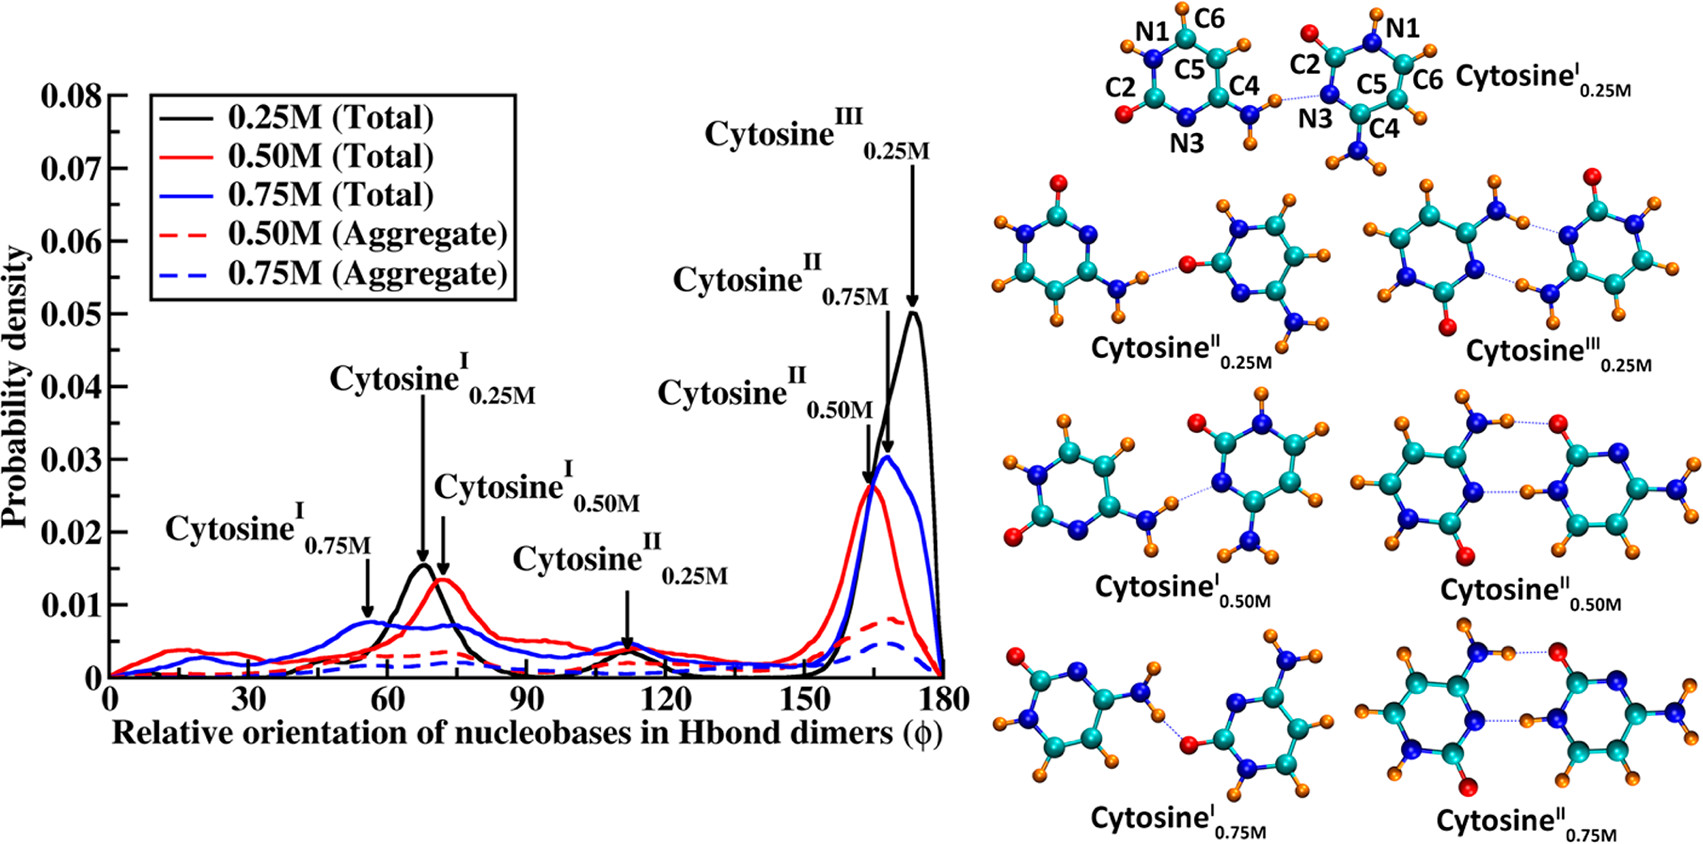
\includegraphics[width=\textwidth]{Chapter2/Figures/Figure5.png}
    \caption[Probability distribution of the angle between the normal ($\phi$) of the nucleobases involved in hydrogen-bond dimers. Representative images illustrating the arrangement of the nucleobases corresponding to the peaks in the distribution are also presented]{Probability distribution of the angle between the normal ($\phi$) of the nucleobases involved in hydrogen-bond dimers. Representative images illustrating the arrangement of the nucleobases corresponding to the peaks in the distribution are also presented. Atom numbering is also presented to illustrate the atoms involved in the hydrogen-bond. Dotted curves in the probability distribution correspond to hydrogen-bonded dimers observed in regions (ii) and (iii) of the 0.50 and 0.75 M simulations.}
\end{figure}

We classify the various dimeric assemblies based on the relative orientation of nucleobases within the dimer pairs. The relative orientation of nucleobase in hydrogen-bonded dimers were determined by calculating the angle between the normalized dipole moment vectors ($\phi$) in the identified hydrogen-bonded dimer pairs as discussed earlier for the solution simulation. The probability distribution of the relative orientation is presented in Figure 4.7. The atoms involved in various hydrogen-bonded dimers are presented in Table 4.1.
\begin{table}
    \centering
    \caption[Atoms involved in the hydrogen-bonds for the various structures observed in the nucleobase - graphene simulations]{Atoms involved in the hydrogen-bonds for the various structures observed in the nucleobase - graphene simulations}
    \begin{tabular}{cccc}
        \toprule
        Structure   &   Nucleobase I    &   Nucleobase II     &     Orientation \\ \midrule
        Cytosine\textsuperscript{I}\textsubscript{0.25M}    &   -NH\textsubscript{2}    &   C2(O)   &   72$\degree$ \\
        Cytosine\textsuperscript{II}\textsubscript{0.25M}   &   C2(O)   &   N1      &   115$\degree$    \\
        Cytosine\textsuperscript{III}\textsubscript{0.25M}  &   N3      &   C2(O)   &   173$\degree$    \\
                                                            &   C2(O)   &   N3      &   \\
        Cytosine\textsuperscript{I}\textsubscript{0.50M}    &   N3      &   -NH\textsubscript{2}    &   73$\degree$ \\
        Cytosine\textsuperscript{II}\textsubscript{0.50M}   &   -NH\textsubscript{2}    &   C2(O)   &   164$\degree$    \\
                                                            &   N3      &   N1      &   \\
        Cytosine\textsuperscript{I}\textsubscript{0.75M}    &   C2(O)   &   -NH\textsubscript{2}    &   60$\degree$ \\
        Cytosine\textsuperscript{II}\textsubscript{0.75M}   &   -NH\textsubscript{2}    &   C2(O)   &   166$\degree$    \\
                                                            &   N3      &   N1      &   \\  \bottomrule
    \end{tabular}
\end{table}

For the low (0.25 M) concentration limit, we observed the formation of three distinct dimer pairs, with average relative orientations of 72$\degree$ (Cytosine\textsuperscript{I}\textsubscript{0.25M}), 115$\degree$ (Cytosine\textsuperscript{II}\textsubscript{0.25M}), and 173$\degree$ (Cytosine\textsuperscript{III}\textsubscript{0.25M}). The dimer pairs with relative orientations of 72 and 115$\degree$ were observed to be transient structures with a single hydrogen bond between the interacting residues. Cytosine\textsuperscript{III}\textsubscript{0.25M} is stabilized by the formation of two symmetric hydrogen bonds between C2(O) and the N3 nitrogen of the interacting nucleobases. The Cytosine\textsuperscript{III}\textsubscript{0.25M} structure agrees with the kk2 structure previously reported by Fernandez et al.\supercite{gonzalez_competition_2017} and was also observed to be a part of C1-D(2) type ribbon structures for cytosine networks studied by Otero et al.\supercite{otero_elementary_2008} using STM imaging and DFT calculations. The dimer pairs Cytosine\textsuperscript{I}\textsubscript{0.25M} and Cytosine\textsuperscript{III}\textsubscript{0.25M} were previously observed by us from short simulations of cytosine nucleobases on graphene sheets.\supercite{h_polarization_2021} 

For intermediate (0.50 M) concentrations, we observe the formation of two distinct dimer pairs, with relative average orientations of 72$\degree$ (Cytosine\textsuperscript{I}\textsubscript{0.50M}) and 164$\degree$ (Cytosine\textsuperscript{II}\textsubscript{0.50M}). Cytosine\textsuperscript{I}\textsubscript{0.50M} appears as a transient structure with only one hydrogen-bond between the nucleobases. Cytosine\textsuperscript{II}\textsubscript{0.50M} was observed to be stabilized by two hydrogen bonds between the residues, with hydrogen bonds forming between the amino (-NH\textsubscript{2}) group and C2(O) and between the N3 and N1 nitrogen atoms. The structure assigned as Cytosine\textsuperscript{II}\textsubscript{0.50M} agrees with the structure kk1 previously reported by Fernandez et al. using REMPI spectroscopy and MM/DFT studies.\supercite{gonzalez_competition_2017} At high concentration (0.75M) limits, we observe the formation of two unique dimer pairs, with relative orientations of 60$\degree$ (Cytosine\textsuperscript{I}\textsubscript{0.75M}) and 166$\degree$ (Cytosine\textsuperscript{II}\textsubscript{0.75M}). The dimer pair with a relative average orientation of 166° (Cytosine\textsuperscript{II}\textsubscript{0.75M}) is structurally similar to the dimer pair Cytosine\textsuperscript{II}\textsubscript{0.50M}, with both structures being stabilized by two pairs of hydrogen bonds between the interacting nucleobases. Thus, from the nucleobase - graphene simulations we observe the formation of a dominant hydrogen-bonded dimer pair with relative orientation of $\phi$ $\geq$ 160$\degree$. This alludes to the effect of the underlying graphene sheet in stabilizing the interactions between the nucleobases by providing a solid support for the formation of planar/quasi-planar hydrogen-bonded dimers. However, we also note the gradual decrease in the probability of formation of planar/quasi-planar dimers with the increase in the concentration of nucleobases. In Figure 4.7, we also present the relative orientation of nucleobases in hydrogen-bonded dimers observed in the aggregate regions (ii) and (iii) from the 0.50 and 0.75 M simulations. We observe that the distribution is spread from 0 to 180$\degree$. Thus, at low concentrations we observe the formation of an ordered 2D assembly while at higher concentrations we see a shift toward complex 3D assembly of nucleobases. We notice that the hydrogen-bonded dimer distributions observed in the nucleobase - graphene simulations are very different from the distributions observed in the 0.60 M nucleobase only simulations. This is due to the differences in the binding energetics observed in the nucleobase - graphene and nucleobase - nucleobase systems. In our earlier study, we reported the $\pi$-stacking binding free energies between nucleobase - graphene and nucleobase - nucleobase to be -7.87 and 0.66 kcal/mol, respectively, while the nucleobase - nucleobase hydrogen-bonding free energy was estimated to be -2.03 kcal/mol. Thus, in a nucleobase - graphene system the nucleobases favor adsorption onto the graphene sheet followed by hydrogen-bonding between the nucleobases, while in a nucleobase-only system hydrogen-bonding is favored over formation of $\pi$-stacks, thereby resulting in the observed differences in the hydrogen-bonding patterns.
\begin{figure}
    \centering
    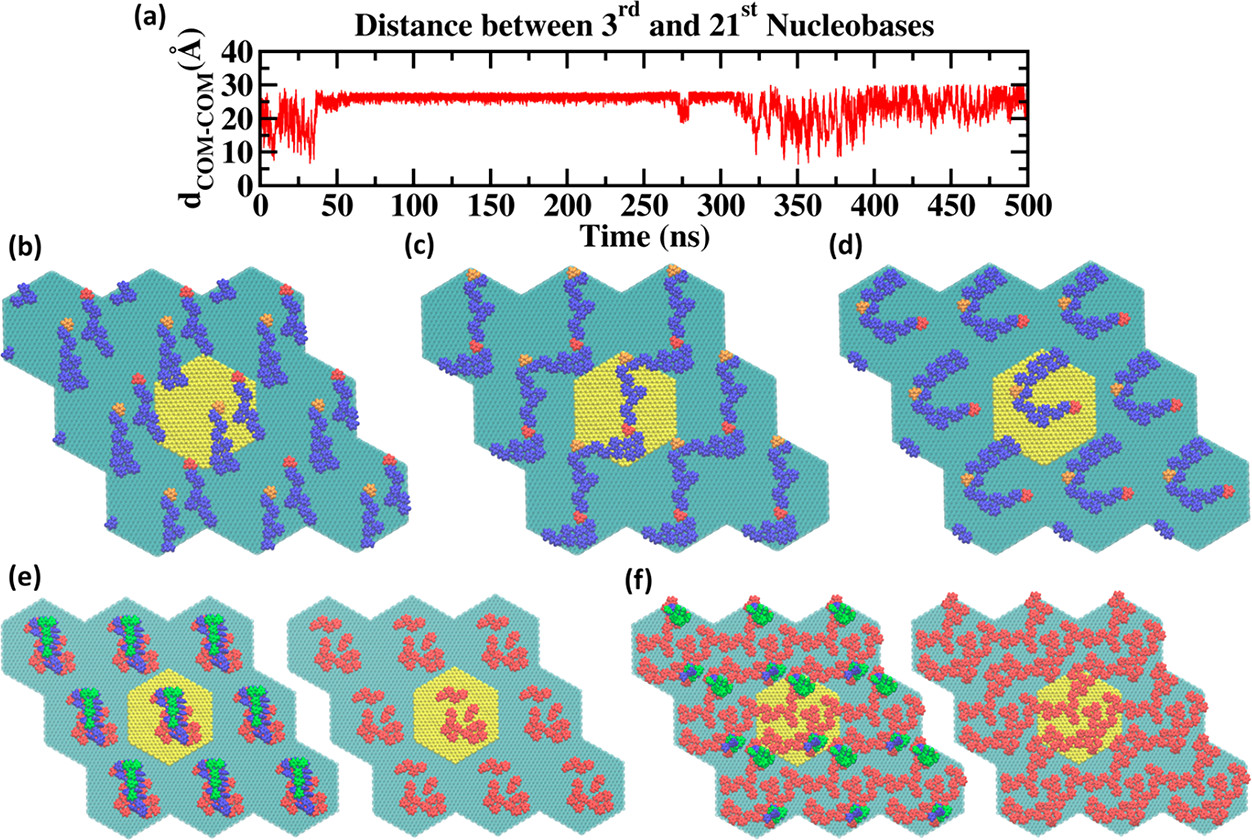
\includegraphics[width=\textwidth]{Chapter2/Figures/Figure6.png}
    \caption[Time series of the center-of-mass to center-of-mass descriptor used to identify the nucleobase assemblies observed in 0.25 M simulations. Representative structures depicting the 2D network corresponding to different regions of the d\textsubscript{COM-COM} time series. Representative structures of nucleobase assemblies in 0.50 M and 0.75 M simulations]{(a) Time series of the center-of-mass to center-of-mass descriptor used to identify the nucleobase assemblies observed in 0.25 M simulations. Representative structures depicting the 2D network corresponding to (b) region-I, (c) region-II, and (d) region-III of the d\textsubscript{COM-COM} time series. Representative structures of nucleobase assemblies in (e) 0.50 M and (f) 0.75 M simulations. The simulation cell is indicated in yellow color and periodic images of the cell are colored green. (b-d) Nucleobases used in the center-of-mass metric are in red (3) and orange (21). All other nucleobases are colored blue. (e) and (f) Nucleobases are color-coded with respect to the distance from the graphene sheet. Nucleobases in regions (i) (d\textsubscript{Nuc-Graph} < 4.5 $\angstrom$), (ii) (4.5 $\angstrom$ < d\textsubscript{Nuc-Graph} < 8.5 $\angstrom$), and (iii) (d\textsubscript{Nuc-Graph} > 8.5 $\angstrom$) are presented in red, blue, and green, respectively.}
\end{figure}

Cytosine nucleobases are known to form hydrogen-bonded assemblies on 2D supports like Au(111),\supercite{kelly_understanding_2008, otero_elementary_2008} Cu(111), and HOPG.\supercite{xu_directional_2021} Having analyzed the relative orientations of nucleobases in the hydrogen-bonded dimers observed in the nucleobase - graphene sheet simulations, we next analyze the formation of two-dimensional network structures in these simulations. Inspection of the simulation trajectory reveals the formation 2D assemblies for the low concentration limit of 0.25 M, while 3D structures are observed for 0.75 M. This is also visible in the representative images presented in Figure 4.2. To identify the network structures, we employed the distance between the center of mass of two selected nucleobases (d\textsubscript{COM-COM}) as the metric to analyze the formation of such networks. The nucleobases were chosen in such a fashion that the COM-COM distance between them was able to accurately capture the dynamics of the 2D network under consideration. For the 0.25 M simulation, we employed the COM-COM distance between the 3\textsuperscript{rd} and 21\textsuperscript{st} nucleobases to describe the dynamics of the network. We present the d\textsubscript{COM-COM} time series corresponding to the selection in Figure 4.8(a). From the d\textsubscript{COM-COM} time series, we observe three distinct time series blocks wherein separate network structures exist. We denote the three blocks as follows: Region-I, corresponding to the initial 50 ns of the analyzed trajectory; Region-II, corresponding to the 50-300 ns window, and Region-III, corresponding to the last 200 ns of trajectory. We observe that for the initial 50 ns of the analyzed trajectory, the COM-COM distance oscillates around an average value of 20 $\angstrom$. In this region, we observe the formation of two different clusters which are in constant motion. This is depicted in the representative structure presented in Figure 4.8(b). After the initial 50 ns, the COM-COM distance quickly settles to an average distance of 25 $\angstrom$. This distribution persists to the last 200 ns. In this region we observe the formation of a periodic zigzag ribbon structure that spans across the periodic boundary conditions of the simulation cell. This is illustrated by the representative structure presented in Figure 4.8(c). Beyond 300 ns, we again observe fluctuations in the distance distribution. The periodic network structure breaks away and leads to the formation of island structures, as illustrated by the representative structure presented in Figure 4.8(d). Both the long network structures as well as the island structures have been observed in experimental studies and by STM imaging of cytosine nucleobases adsorbed on metal surfaces such as Au(111).\supercite{kelly_understanding_2008,wandlowski_structure_1996,iakhnenko_adsorption_2013,hsu_stm_2021}

Upon increasing the concentration of the nucleobases, we observe an increase in the $\pi$-$\pi$ interaction between the nucleobases, as the monolayer assembly is replaced by multiple layers. The 2D periodic network structure is lost and is replaced by a 3D arrangement of nucleobases favored by interaction between $\pi$-stacks. In Figure 4.8(e), we present the representative structure of the clustered assembly of the nucleobases. The various stacks are presented to highlight the formation of 3D layered structures. For the 0.50 M simulations, the nucleobases are dispersed in various layers. Upon increasing the concentration to 0.75 M, we saturate the graphene sheet with nucleobases, which results in the formation of a pseudoperiodic assembly of the nucleobases in addition to the formation of 3D layered structures. This is reflected in the representative structure presented in Figure 4.8(f).
\begin{figure}
    \centering
    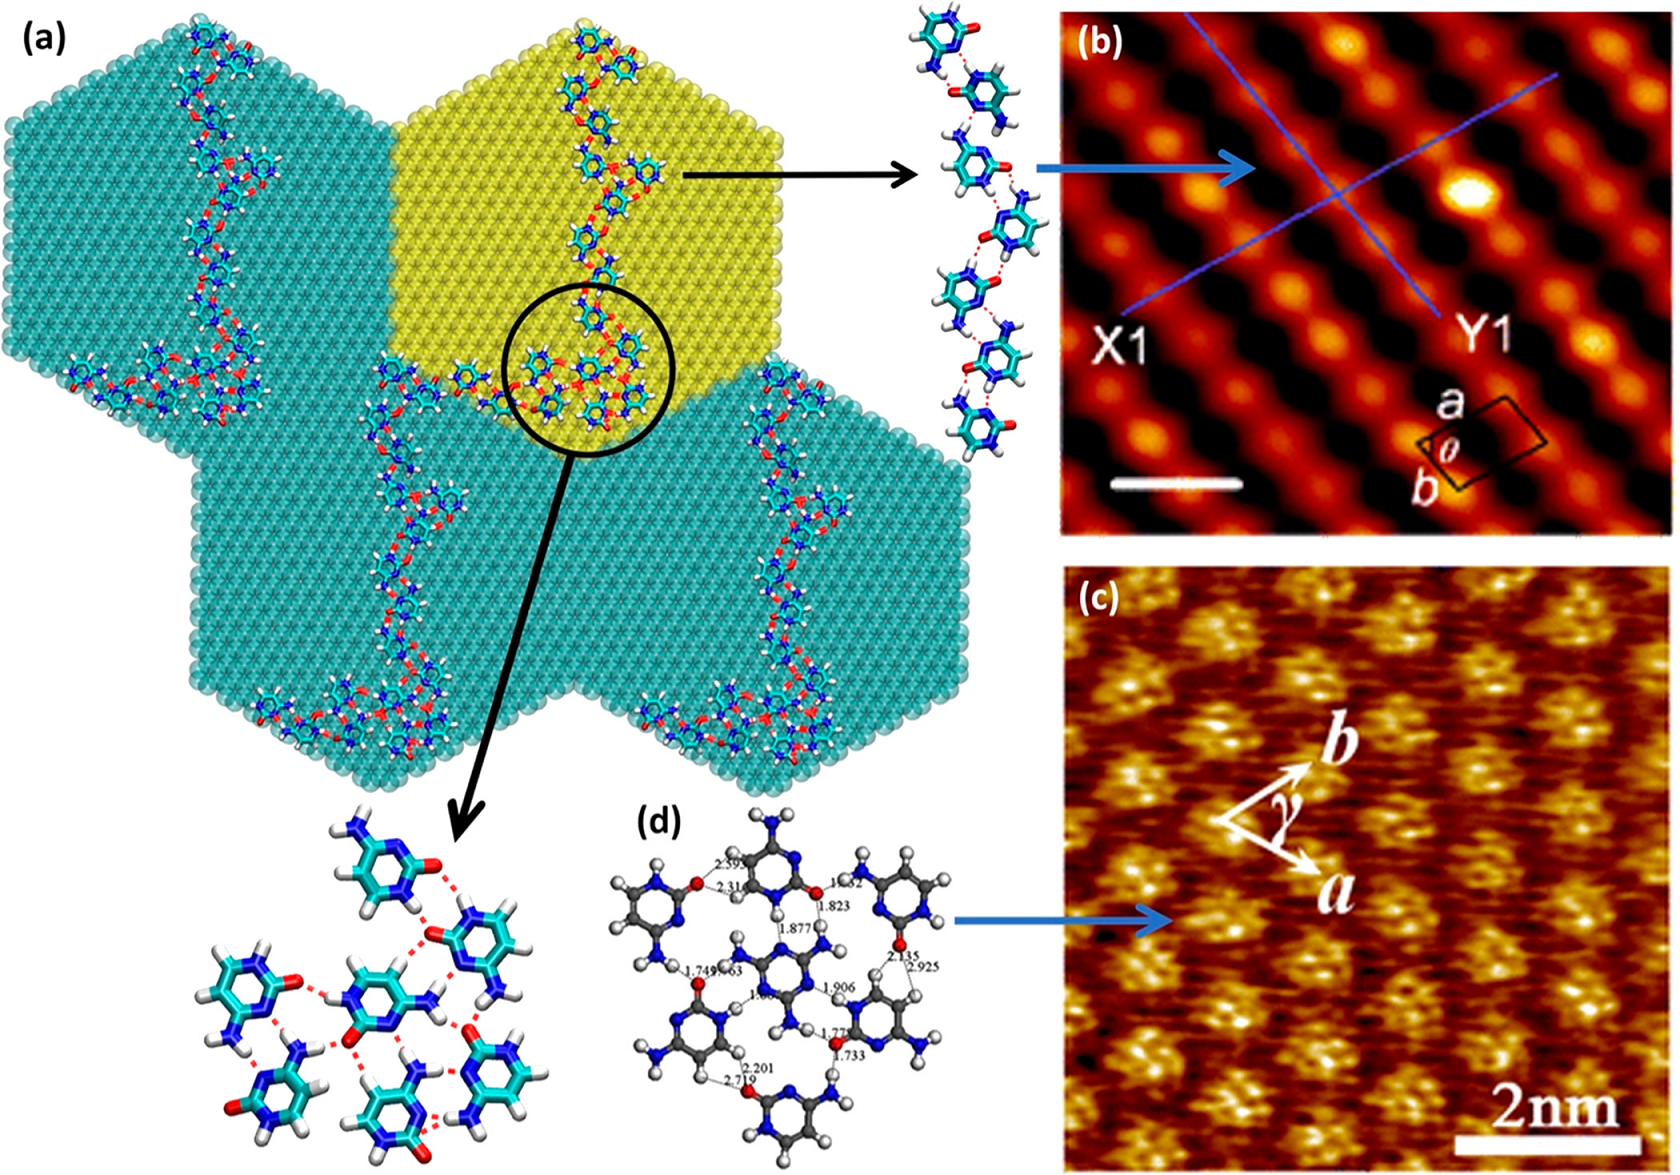
\includegraphics[width=\textwidth]{Chapter2/Figures/Figure7.png}
    \caption[Hydrogen-bonded networks observed in the periodic structure in monolayer assemblies stabilized by the two specific patterns, linear zigzag structures and circular hexagonal arrangement. HR-STM images from experimental reports are also presented]{(a) Hydrogen-bonded networks observed in the periodic structure in monolayer assemblies stabilized by the two specific patterns, linear zigzag structures and circular hexagonal arrangement. (b) HR-STM image (5 × 5 nm2, scale bar, 1 nm) of pure cytosine at the 1-octanol/HOPG interface. Image adapted with permission from ref. \supercite{xu_coadsorption_2006}. Copyright 2022 American Chemical Society. (c) HR-STM for self-assembled domain of melamine-cytosine coassembly. (d) Dmol3 calculated structure of the proposed hexagonal arrangement with six cytosine nucleobases surrounding a central melamine molecule. (c) and (d) Adapted from ref. \supercite{zhao_investigating_2016} under the terms of the Creative Commons Attribution 4.0 International License (http://creativecommons.org/licenses/by/4.0/).}
\end{figure}

In Figure 4.9(a), we present a detailed view of the hydrogen-bonded assemblies that stabilize the periodic monolayer assembly. We notice the formation of a central node which comprises of seven nucleobases arranged in a circular hexagonal fashion. These nodes are connected to an arm-type arrangement that is facilitated by the zigzag linear arrangement of the cytosine nucleobases. It is noted that these assemblies are stabilized by both symmetric and asymmetric hydrogen-bonds between the nucleobases. These arrangements have been have observed for cytosine nucleobases adsorbed on liquid/solid 1-octanol/HOPG interfaces.\supercite{zhao_investigating_2016,xu_coadsorption_2006} Pure cytosine adsorbed at the 1-octanol/HOPG interface is found to be arranged in the linear zigzag fashion. This was investigated by Xu et al. using high-resolution STM (HR-STM). In Figure 4.9(b), we reproduce the high-resolution STM image of pure cytosine adsorbed at the 1-octanol/HOPG interface, wherein the zigzag arrangement of the bases is clearly observed.\supercite{xu_coadsorption_2006} Zhao et al. studied the coadsorption of melamine and cytosine at the 1-octanol/HOPG interface using HR-STM. They found the formation of distorted hexagonal molecular-assembled island structures. We reproduce the HR-STM images obtained by Zhao et al. in Figure 4.9(c).\supercite{zhao_investigating_2016} Using DFT calculations, they ascribed the hexagonal assembly to a melamine molecule surrounded by six cytosine molecules. In Figure 4.9(d), we reproduce the calculated structure proposed by Zhao et al.\supercite{zhao_investigating_2016} We observe that the circular node structure observed by us, wherein a central cytosine is surrounded by six other cytosine nucleobases, is similar to the arrangement of the central melamine surrounded by six cytosine nucleobases. This direct correlation of our simulations with experimentally realized molecular arrangements highlights the strength of polarizable simulations in capturing the self-assembly of nucleobases on 2D graphene support.
\section{Conclusions}
In conclusion, we have investigated the influence of concentration on the self-assembly behavior of nucleobases on a 2D graphene support. The study sheds light on the dynamics of multilayered self-assemblies, hitherto unexplored in the literature, by the inclusion of polarization into simulations. The accurate description of the various interactions forces (Hydrogen-bonded and $\pi$-stacking) allowed us to study the evolution of the dynamics of the system.  At low concentrations (0.25 M), $\pi$-stacking interactions between the graphene surface and nucleobases were found to drive the dynamics of the system. At an intermediate concentration (0.50 M), we observe competition between graphene - nucleobases $\pi$-stacking interactions and nucleobase - nucleobase interactions, leading to the formation of multilayered assemblies. This resulted in the formation of a 3D aggregate structure tethered to the graphene sheet. At a high concentration limit (0.75 M), which is closer to the surface loading limit, our study captures the formation of pseudo-2D assemblies of the nucleobases on the graphene sheet that support 3D aggregate assemblies. This reflects a transition toward glassy networks. These observations are consistent with the experimental observation of cytosine nucleobases adsorbed on 1-octanol/HOPG solid-liquid interfaces and Au(111) surfaces,\supercite{kelly_understanding_2008, wandlowski_structure_1996, zhao_investigating_2016, xu_coadsorption_2006} where such glassy networks were observed via HR-STM imaging. In conclusion, we show that a generalized polarizable FF can accurately capture the formation of self-assembled structures, without the need for specific interaction potentials. We believe that this study would pave the way for further studies on small-molecule assemblies with applications in nanopatterning and tailored self-assemblies. The study will also serve as a benchmark for the applicability of polarizable simulations in capturing solid-liquid interfacial phenomenon.
    \chapter[Capturing Charge and Size Effects of Ions at the Graphene - Electrolyte Interface Using Polarizable Force Field Simulations]{Capturing Charge and Size Effects of Ions at the Graphene - Electrolyte Interface Using Polarizable Force Field Simulations \protect\footnote[4]{This chapter has been published as \textbf{H., Hemanth}, Mewada, R. and Mallajosyula*, S.S.; Capturing Charge and Size Effects of Ions at the Graphene - Electrolyte Interface Using Polarizable Force Field Simulations; {\textit{Nanoscale Adv.}, 2023, \textbf{5}, 796 - 804}}}
\section{Introduction}
Graphene, a 2D allotrope of carbon with a hexagonal unit cell and layered architecture has attracted significant attention from the scientific community with applications in varied fields such as desalination,\supercite{sun_selective_2014,joshi_precise_2014,homaeigohar_graphene_2017,boretti_outlook_2018,yang_ultrathin_2017} energy storage\supercite{liang_graphene-based_2009,wang_supercapacitor_2009,wang_sngraphene_2009,stoller_graphene-based_2008} and electrochemical sensing.\supercite{sheng_electrochemical_2012,pumera_graphene_2010,pumera_electrochemistry_2009} For example, by tuning the interlayer separation in graphene-oxide (GO) membranes Abraham et al. achieved near-perfect salt-rejection, establishing the applicability of graphene and graphene-oxide based membranes for desalination.\supercite{abraham_tunable_2017,nair_unimpeded_2012} For technological advancement in these applications, it is important to understand the adsorption behaviour of the constituent ions at the electrolyte - graphene interface. It is to be noted that simple theories based on the continuum model, which consider only the size and the magnitude of the charge, cannot capture the dynamics of the ion - surface interactions. The shortcomings of the continuum model are even more pronounced for hydrophobic surfaces as observed in graphene and GO sheets, where the interactions are not purely electrostatic.\supercite{mennucci_polarizable_2002} Experimental studies using deep UV second harmonic generation measurements found that direct ion - graphene interactions were responsible for the adsorption of SCN\textsuperscript{-} ions on the graphene surface, with the interactions being enthalpically driven.\supercite{mccaffrey_mechanism_2017} A simple continuum model fails to capture these effects. It has been noted that the adsorption of ions on hydrophobic surfaces is affected by various properties of the ions, including their size, polarizability and hydration free energy to name a few.\supercite{iamprasertkun_capacitance_2019,glendening_dicationwater_1996} Gaining molecular insight into the governing mechanisms of ion-adsorption requires accurate modelling of the electrolyte - graphene interface.

QM calculations can accurately predict such properties, but the scaling of O(\textit{N\textsuperscript{3-4}}) for DFT calculations limits the applicability of such methods to very small systems.\supercite{mu_hydrated_2021} In one such study the interaction of hydrated cation clusters (cation-(H\textsubscript{2}O)\textsubscript{7}) with a graphene sheet was studied which revealed reorganization of the hydration shell around K\textsuperscript{+}, allowing K\textsuperscript{+} to directly interact with the graphene sheet, while such reorganization of the hydration shell was not observed for Li\textsuperscript{+}.\supercite{mu_hydrated_2021} These static QM calculations were followed by very short (10 ps) AIMD simulations to comment on the hydration dynamics.\supercite{mu_hydrated_2021,li_unraveling_2015} These studies highlight the need for alternative methods to accurately capture the ion - graphene interaction in aqueous environments.

Molecular dynamics (MD) simulations offer a viable solution to such problems. However, MD simulations based on classical additive force fields (FFs) cannot capture the ion - graphene interactions as they do not account for charge transfer. Gas-phase and polarizable continuum model (PCM) calculations have shown that the polarizability of ions and the surface plays an important role in describing the strength and evolution of the ion - graphene interactions.\supercite{sunner_ion-solvent_1981,zhou_deciphering_2020} Based on these facts efforts have been focused towards the development of FF parameters that can describe the interactions between ions and the graphene surface.\supercite{williams_effective_2017,chen_multiscale_2018} In these studies, an additional force field term is added to describe the ion - graphene interactions. The parameters are empirically tuned to reproduce the QM calculated binding energies, thus enabling additive simulations to capture the ion - graphene interactions in an otherwise non-polarizable FF simulation.\supercite{williams_effective_2017,chen_multiscale_2018} One of the major drawbacks of such implementations is that the target DFT calculations used to tune the ion - graphene interactions overemphasize the binding energetics as they are based on a mean-field description of the solvation rather than explicit solvation.

To this end polarizable simulations offer a framework for studying the evolution of ion - graphene interactions in explicit solvent, negating the need to empirically tune the FF parameters.\supercite{lin_polarizable_2018,h_polarization_2021}  In our earlier work we described the development and testing of Drude parameters to describe multilayer and monolayer graphene surfaces.\supercite{h_polarization_2021,h_capturing_2022} Here, we study the energetics and dynamics of an aqueous salt solution - multilayer graphene system using Drude polarizable FF simulations, to critically evaluate the ability of FF parameters in describing the interfacial phenomenon.

\section{Computational Methodology}
Multilayer graphene comprising four graphene sheets with a radius of 15 $\angstrom$ and combined height of 10.04 $\angstrom$, where height corresponds to the distance between the lower graphene sheet and the top-most graphene sheet, was modelled using the Inorganic Builder plugin available in the Visual Molecular Dynamics (VMD) package.\supercite{humphrey_vmd_1996} The graphene sheets were stacked in `ABAB` arrangement to simulate multilayer graphene. The multilayer graphene was solvated to bring the final system dimensions to (29.42 x 29.42 x 45)$\angstrom$\textsuperscript{3}. We introduced one molecule (one mole) of the salt of interest (NaCl, KCl, MgCl\textsubscript{2}, CaCl\textsubscript{2} and CsCl) to the solvated system using the AutoIonize plugin available in VMD. We present a representative image of the system setup in Figure 5.1. The Chemistry at Harvard Molecular Mechanics (CHARMM36) all-atom force field (FF) was used to describe bonded and non-bonded interactions in graphene sheets and ions.\supercite{vanommeslaeghe_charmm_2009} A TIP3P three-point water model\supercite{jorgensen_comparison_1983} was used to describe water molecules in additive FF simulations.

We employed in-house scripts to add Drude particles to the final systems to generate the corresponding Drude FF files. The classical Drude oscillator polarizable FF hereto referred to as the Drude polarizable FF was used to describe non-bonded interactions in ions.\supercite{lin_polarizable_2018,h_polarization_2021} Drude polarizable FF parameters previously tested by us were used to describe bonded and non-bonded interactions in graphene sheets.\supercite{h_polarization_2021} The SWM4-NDP polarizable water model\supercite{lamoureux_polarizable_2006} was used to describe water molecules in Drude polarizable FF simulations. We restrained the bond lengths and bond angles in water molecules using the SETTLE algorithm\supercite{miyamoto_settle_1992} in Drude polarizable FF simulations.

Molecular dynamics simulations were performed using the Nanoscale Molecular Dynamics (NAMD) package\supercite{phillips_scalable_2005,phillips_scalable_2020} in an isobaric-isothermal (NPT) ensemble. Particle mesh Ewald\supercite{darden_particle_1993} (PME) summation was used to evaluate the electrostatic interactions with a real-space cut-off of 9 $\angstrom$. All simulations were performed under NTP conditions (298 K and 1 atm pressure) with Langevin dynamics and the Nos\'{e}-Hoover Langevin piston to maintain the NTP conditions. We employed an additional dual thermostat at 1 K to maintain the Drude particles at 1 K during Drude polarizable FF simulations. All systems were minimized for 4000 steps and equilibrated for 1 ns in NPT and 1 ns in NVT ensembles respectively. The central atom of the graphene sheet was restrained using a harmonic potential of 1 kcal mol\textsuperscript{-1} $\angstrom$\textsuperscript{-2} to arrest the sliding motion of the graphene sheets. No additional restraints were employed during the simulations, and the sheets were allowed to relax and breathe during the simulations. We had previously shown that constraining the graphene surface affects the energetics of the system.\supercite{h_polarization_2021} The equations of motion were integrated using a time step of 1 fs in additive FF simulations and 0.5 fs in Drude polarizable FF simulations. Production simulations were performed for a total of 100 ns for each of the six salt - graphene systems considered.

We performed simulations using adaptive biasing force (ABF) to estimate the binding free energies for ion - graphene interactions. ABF scans were performed in a window spanning 3 $\angstrom$ to 15 $\angstrom$ above the topmost graphene sheet. A biasing force of 0.20 kcal mol\textsuperscript{-1} $\angstrom$\textsuperscript{-2} was employed at both ends of the scan length. The scan window was divided into bins of 0.05 $\angstrom$ length. The ABF runs were performed in a hexagonal cell of dimensions (29.42 x 29.42 x 45) $\angstrom$\textsuperscript{3}. ABF runs were performed for a total of 100 ns, and the runs were deemed convergent when the number of observations in each bin was >1.5 x 10\textsuperscript{6}. The methodology for the calculation of ABF was adopted from the work by Comer et al.\supercite{comer_predicting_2015,poblete_determinants_2017}

The densities of ions and water at the graphene - ion interfaces were calculated using in-house scripts. Densities were computed in a window spanning 15 $\angstrom$ from the surface of the multilayer graphene. The calculation window was divided into bins of 0.1 $\angstrom$ length, and the number of observations in each bin was computed. 

% Instantaneous dipole moments for the ions were computed from the simulation trajectory using in-house codes. We calculated the vibration of the Drude particles associated with each ion over the entire simulation trajectory, and the dipole moment for each ion-Drude particle pair was computed as the vector sum of the charge of the particles (ion and the Drude particle) times the distance towards the particle from the combined center of mass of the ion-Drude particle system. The dipole moments are computed in local coordinate frames, such that the center of mass of the ion - Drude particle system is placed at origin. 

% Average dipole moments for the patches of graphene surface interacting with the ions were computed using in-house codes. Similar to the calculation of the dipole moments associated with the ions, we first iterated over all the ions present in the system, and for each ion, a cylindrical selection of carbon atoms was made, with the radius of the cylinder set to 4 $\angstrom$ and the height of the cylinder set to 14 $\angstrom$. This initial selection was then post-processed to remove water molecules and other ions that might be present, to generate the patch of graphene surface directly interacting with the ion. The dipole moment for the graphene patch was then computed as a vector sum of the charge of the particles (carbon atomand the associated Drude particle) times the distance towards the particle from the combined center of mass of the carbon atom - Drude particle system. It is important to note that the vector sum is calculated over all the carbon atoms present in the patch, with the coordinate frame shifted to each carbon atom in sequence.

\section{Results and Discussions}
\begin{figure}
    \centering
    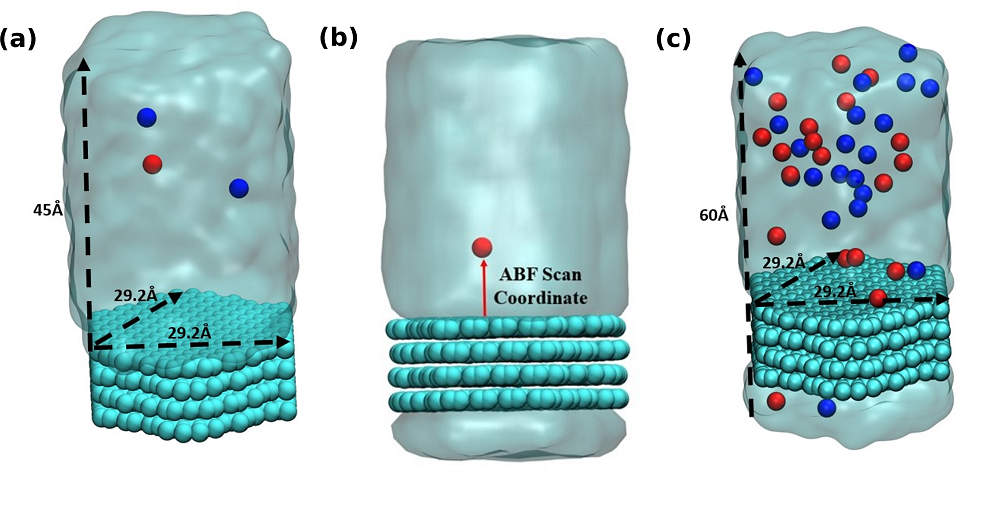
\includegraphics[width=\textwidth]{Chapter3/Figures/FigureS1.png}
    \caption[Representative structures depicting system setup for various systems investigated in this study]{(a) Representative structure depicting system setup for ABF simulations, (b) Scan coordinate used in ABF simulations, and (c) Representative structure for 1M salt solution runs. Lattice vectors for the multilayer graphene are indicated.All figures are prepared using VMD\supercite{humphrey_vmd_1996}.}
\end{figure}

Before discussing the characteristics of the ion - graphene interactions at the graphene - solvent interface we first establish the energetics of ion - graphene interactions.  To this end, we calculate the binding free energy for Li\textsuperscript{+}, Na\textsuperscript{+}, K\textsuperscript{+}, Cs\textsuperscript{+}, Mg\textsuperscript{2+}, Ca\textsuperscript{2+} and Cl\textsuperscript{-} using ABF (adaptive biasing force) simulations for both polarizable and additive force fields. We chose four monovalent cations (Li\textsuperscript{+}, Na\textsuperscript{+}, K\textsuperscript{+}, and Cs\textsuperscript{+}) and two divalent cations (Mg\textsuperscript{2+} and Ca\textsuperscript{2+}) to evaluate the influence of size and charge on the binding free energetics. Cl\textsuperscript{-} is used as the common counterion.  For the ABF simulations we use one molecule of the salt of interest in the solution. Representative images depicting the system setup for ABF simulations are presented in Figure 5.1(a). We employed the z-axis projection of the center-of-mass distance between the ions of interest and the top layer of the multilayer graphene as the scan coordinate. The scan coordinate used for the ABF simulations is presented in Figure 5.1(b). We present the potential of mean force (PMF) scans obtained from Drude polarizable and additive simulations for the monovalent cations in Figure 5.2 and for divalent cations and Cl\textsuperscript{-} ions in Figure 5.3. We also present the binding free energies obtained from Drude polarizable and additive FF simulations in Table 5.1. The binding free energies were estimated with respect to the minimum in the PMF scan and the well separated structure. For the monovalent ions, Li\textsuperscript{+}, Na\textsuperscript{+}, K\textsuperscript{+} and Cs\textsuperscript{+}, the binding free energies from Drude polarizable (additive) FF simulations are estimated to be -6.91 (-7.84), -5.83 (-1.10), -7.13 (-0.56) and -13.26 (-5.38). All energies are reported in kJ mol\textsuperscript{-1}. In Table 5.1 we also report the difference ($\Delta$E\textsubscript{1}) between the Drude polarizable and the additive binding energies. $\Delta$E\textsubscript{1} for Li\textsuperscript{+}, Na\textsuperscript{+}, K\textsuperscript{+} and Cs\textsuperscript{+} is observed to be 0.93 kJ mol\textsuperscript{-1}, -4.73 kJ mol\textsuperscript{-1}, -6.57 kJ mol\textsuperscript{-1} and -7.88 kJ mol\textsuperscript{-1} respectively.  We observe that except for Li\textsuperscript{+} the binding free energies estimated from Drude polarizable simulations are higher than the corresponding values obtained from the additive simulations. This indicates a stronger binding between the graphene surface and the monovalent ions in Drude polarizable simulations when compared to the additive simulations.  Earlier efforts to study ion - graphene interactions using MD simulations relied on capturing DFT derived binding profiles.\supercite{williams_effective_2017,chen_multiscale_2018} These have been found to overestimate the binding energetics.\supercite{elliott_qmmd_2020} We present a comparison of the binding free energies obtained by us with those obtained in these earlier studies to put the values obtained by us into perspective.  In Table 5.1 we present the adsorption energies estimated by Carbone et al. using CPCM DFT calculations (E\textsubscript{DFT}) and from PMF scans obtained after tuning the additive FF parameters (E\textsubscript{additive}\textsuperscript{\#}) to reproduce the CPCM DFT calculations. The E\textsubscript{additive}\textsuperscript{\#} values for Li\textsuperscript{+}, Na\textsuperscript{+} and K\textsuperscript{+} were reported to be -10.7 kJ mol\textsuperscript{-1}, -14.5 kJ mol\textsuperscript{-1} and -12.3 kJ mol\textsuperscript{-1}. The values obtained by us using the Drude polarizable FF are lower than those estimated by Carbone et al. In a follow up study Carbone et al. highlighted two potential shortcomings of the Lennard-Jones parameters optimized by them: (i) the model was parametrized using a single ion thereby the effect of ionic screening due to multiple ions was only included via the standard Lorentz-Berthelot combination rules and (ii) the model did not account for the polarization of the graphene surface due to the specific arrangement of the water molecules at the interface.\supercite{elliott_qmmd_2020} We note that these effects might have contributed to the very high adsorption energies observed by Carbone et al. DFT typically overestimates the adsorption of the ions onto the graphene sheet as it does not account for the screening of the charges by the water molecules. Fang et al. studied the interaction of hydrated cations, Li\textsuperscript{+}-(H\textsubscript{2}O)\textsubscript{n}, Na\textsuperscript{+}-(H\textsubscript{2}O)\textsubscript{n} and K\textsuperscript{+}-(H\textsubscript{2}O)\textsubscript{n} with the graphene sheet.\supercite{mu_hydrated_2021} The values for Li\textsuperscript{+}-(H\textsubscript{2}O), Na\textsuperscript{+}-(H\textsubscript{2}O) and K\textsuperscript{+}-(H\textsubscript{2}O) were observed to be around -42.0, -35.0 and -29.0 kcal mol\textsuperscript{-1} respectively, while the same for Li\textsuperscript{+}-(H\textsubscript{2}O)\textsubscript{9}, Na\textsuperscript{+}-(H\textsubscript{2}O)\textsubscript{9} and K\textsuperscript{+}-(H\textsubscript{2}O)\textsubscript{9} were observed to be -21.12, -22.27 and -22.98 kcal mol\textsuperscript{-1}. We clearly observe a screening effect upon the inclusion of water which is inversely correlated to the size of the cation; hence parameterizing the FF using a simple screened model would result in overstabilization.\supercite{mu_hydrated_2021} In contrast in the Drude polarizable FF the ions were parametrized to be consistent with aqueous bulk thermodynamic properties, such as hydration free energies, self-diffusion coefficients and the energetics of small ion - water clusters, thereby capturing the screening effects introduced by solvation.\supercite{yu_simulating_2010} This is also reflected in the PMF curves obtained from the Drude polarizable simulations wherein with increasing size of the monovalent cation, we observe signatures of the stabilization of the hydrated species.

\begin{table}
    \centering
    \caption[Binding free energies of ions obtained from Drude polarizable and additive FF ABF simulations. Binding energies from literature are also presented]{Binding free energies of ions obtained from Drude polarizable and additive FF ABF simulations. Binding energies are calculated as the difference between the energies of the equilibrium structure (global minimum) and the well-separated structure. $\Delta E_{1}$ is calculated using the formula $\Delta E_{1}$ = $E_{Drude}$ - $E_{additive}$. $E_{DFT}$ corresponds to the binding free energies obtained by Carbone et al. using CPCM DFT calculations.\supercite{williams_effective_2017} $E_{additive}^{\#}$ corresponds to the binding free energies obtained by Carbone et al. using modified additive FF parameters.\supercite{williams_effective_2017}  Ionic radii in solution.\supercite{marcus_ionic_1988} All energies are presented in kJ mol\textsuperscript{-1}. Radii are presented in $\angstrom$.}
    \begin{tabular}{ccccccc}
        \toprule
        Ion                     &   $E_{Drude}$ &   $E_{additive}$  &   $\Delta E_{1}$  &   $E_{DFT}$\supercite{williams_effective_2017}    &   $E_{additive}^{\#}$\supercite{williams_effective_2017}   &   Ionic Radii\supercite{marcus_ionic_1988} \\ \midrule
        Li\textsuperscript{+}   & -6.91  & -7.84 & 0.93  & -10.4 & -10.7 & 0.71 \\
        Na\textsuperscript{+}   & -5.83  & -1.10 & -4.73 & -13.8 & -14.5 & 0.97 \\
        K\textsuperscript{+}    & -7.13  & -0.56 & -6.57 & -12.6 & -12.3 & 1.41 \\
        Cs\textsuperscript{+}   & -13.26 & -5.38 & -7.88 & —     & —     & 1.73 \\
        Mg\textsuperscript{2+}  & -1.0   & -6.59 & 5.59  & -16.5 & -16.3 & 0.70 \\
        Ca\textsuperscript{2+}  & -2.93  & -1.03 & -1.9  & -15.7 & -16.3 & 1.03 \\
        Cl\textsuperscript{-}   & -5.26  & -5.76 & 0.5   & -6.90 & -7.0  & 1.80 \\ \bottomrule
    \end{tabular}
\end{table}

\begin{figure}
    \centering
    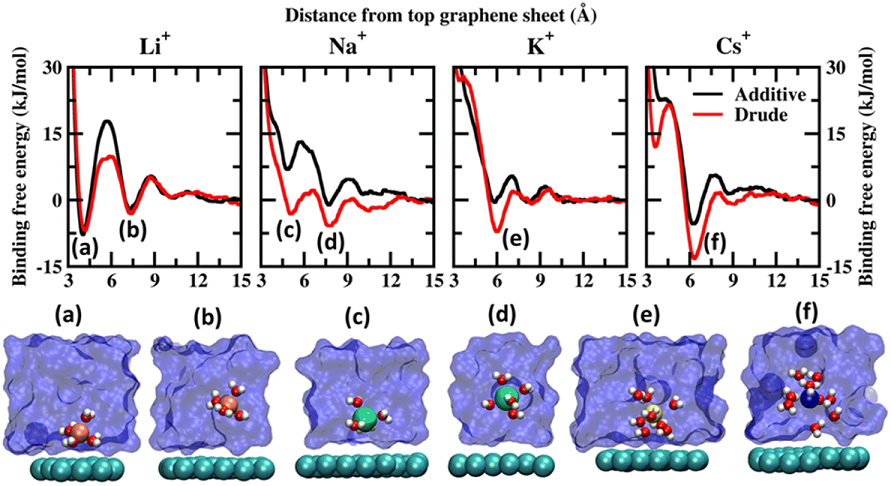
\includegraphics[width=\textwidth]{Chapter3/Figures/Figure2.png}
    \caption[Potential of mean force (PMF) obtained from additive and Drude polarizable FF simulations of monovalent cations considered in this study. Representative structures corresponding to the minima present in the PMF surface obtained from Drude polarizable simulations are also presented to highlight the different interaction modes]{Potential of mean force (PMF) obtained from additive and Drude polarizable FF simulations of monovalent cations, Li\textsuperscript{+}, Na\textsuperscript{+}, K\textsuperscript{+} and Cs\textsuperscript{+}, considered in this study. All energies are reported in units of kJ mol\textsuperscript{-1}. All distances are presented in units of $\angstrom$. Representative structures corresponding to the minima present in the PMF surface obtained from Drude polarizable simulations are presented to highlight the interaction modes. Ions, the underlying graphene sheet and water molecules in the 1\textsuperscript{st} hydration shell are presented in VdW representation. The remaining solvent molecules are presented using a solvent environment to illustrate the solvent environment. Only a small section of the sheet and the solvent are presented for clarity. All figures are prepared using VMD.\supercite{humphrey_vmd_1996}}
\end{figure}

\begin{table}
    \centering
    \small
    \caption[Location of the global minima and next minima observed in the potential energy surface obtained from Drude polarizable and additive PMF simulations]{Location of the global minima and next minima observed in the potential energy surface obtained from Drude polarizable and additive PMF simulations. All distances are presented in units of $\angstrom$.}
    \begin{tabular}{ccccc}
    \toprule
    % Ion         &   Drude Polarizable FF ($\angstrom$)  &               &   additive FF ($\angstrom$)   &                \\
    Ion         &   Minima\textsuperscript{Drude}($\angstrom$)    & Next Minima\textsuperscript{Drude}($\angstrom$)   &   Minima\textsuperscript{add.}($\angstrom$)  &   Next Minima\textsuperscript{add.}($\angstrom$)  \\ \midrule
    Li\textsuperscript{+}                           & 4.20                       & 7.40                     & 4.05                   & 7.25                 \\
    Na\textsuperscript{+}                           & 7.75                       & 5.10                     & 7.75                   & 5.10                 \\
    K\textsuperscript{+}                            & 5.95                       & —                        & 8.10                   & 5.85                 \\
    Cs\textsuperscript{+}                           & 6.35                       & —                        & 6.25                   & —                    \\
    Mg\textsuperscript{2+}                          & 7.55                       & 4.80                     & 4.75                   & 7.46                 \\
    Ca\textsuperscript{2+}                          & 5.95                       & 5.05                     & 7.75                   & 4.70                 \\
    Cl\textsuperscript{-}                           & 3.90                       & —                        & 6.10                   & —                    \\ \bottomrule
    \end{tabular}
    \end{table}

From Figure 5.2, we note that the binding energy curves for all the monovalent ions are predominantly characterized by two minima, the first one at a distance close to $\approx$4 $\angstrom$ and the other minima at a distance $\geq$6 $\angstrom$. These minima correspond to two distinct interaction modes, (i) wherein the ions interact directly with the graphene surface or as a partially solvated species and (ii) wherein the ions interact with the graphene surface through a solvation shell. The distances corresponding to the global minima and the next minima from both the Drude polarizable and additive simulations are tabulated in Table 5.2 for all the systems. For Li\textsuperscript{+}, we observe that the ions favor interacting directly with the graphene sheet at a distance of 4.20 (4.05) $\angstrom$ in Drude polarizable (additive) FF simulations, with binding free energies of -6.91 (-7.84) kJ mol\textsuperscript{-1}. The solvent separated interaction mode is observed at a distance of 7.40 (7.25) $\angstrom$ with binding free energies of -3.09 (-2.10) kJ mol\textsuperscript{-1}. For the remaining monovalent cations Na\textsuperscript{+}, K\textsuperscript{+} and Cs\textsuperscript{+} the solvent separated minima is observed to be the global minima. For Na\textsuperscript{+} ions the global minimum is observed as a solvent separated interaction at a distance of 7.75 $\angstrom$ in both the Drude polarizable and additive simulations. The binding free energy corresponding to this minimum is observed to be -5.83 kJ mol\textsuperscript{-1} and -1.1 kJ mol\textsuperscript{-1} form Drude polarizable and additive simulations respectively.  We observe that the Drude polarizable simulations also favour the direct interaction of the Na\textsuperscript{+} ions and the graphene sheet with a minimum in the binding free energy profile appearing at a distance of 5.10 $\angstrom$, with the binding free energy being -3.15 kJ mol\textsuperscript{-1}. This interaction is not favoured in the additive simulations with the binding free energy being 7.13 kJ mol\textsuperscript{-1}. With increasing size of the ionic radii of the ions we observe the stabilization of the solvent separated minima for both the K\textsuperscript{+} and Cs\textsuperscript{+} species. From the Drude polarizable simulations the minima for K\textsuperscript{+} are observed at 5.95 $\angstrom$, with the binding free energy being -7.13 kJ mol\textsuperscript{-1}. On the other hand, from the additive simulations we observe two shallow minima at 5.85 $\angstrom$ and 8.10 $\angstrom$, with the corresponding binding energy being -0.53 kJ mol\textsuperscript{-1}. For Cs\textsuperscript{+}, a single global minimum is observed at 6.35 $\angstrom$ and 6.25 $\angstrom$ for the Drude polarizable and additive simulations with the binding free energy being -13.26 kJ mol\textsuperscript{-1} and -5.38 kJ mol\textsuperscript{-1} respectively. Overall, for the monovalent ions the binding free energy follows the pattern Cs\textsuperscript{+} > K\textsuperscript{+} > Li\textsuperscript{+} > Na\textsuperscript{+} for the Drude polarizable simulations, while for the additive simulations the pattern is Li\textsuperscript{+} > Cs\textsuperscript{+} > Na\textsuperscript{+} > K\textsuperscript{+}. It can be inferred that the solvent separated interactions are stabilized in the Drude polarizable FF when compared to the additive FF, which is indicative of differential solvation dynamics observed in the Drude polarizable and the additive simulations.

\begin{figure}
    \centering
    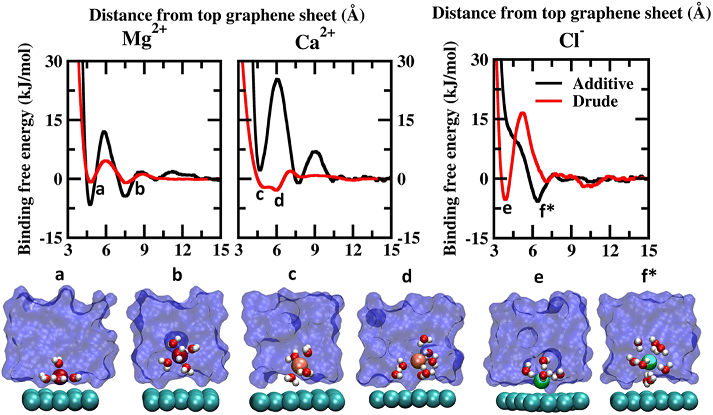
\includegraphics[width=\textwidth]{Chapter3/Figures/Figure3.png}
    \caption[Potential of mean force (PMF) obtained from additive and Drude polarizable FF simulations of divalentvalent cations and Cl\textsuperscript{-} considered in this study. Representative structures corresponding to the minima present in the PMF surface obtained from Drude polarizable simulations are also presented to highlight the interaction modes]{Potential of mean force (PMF) obtained from additive and Drude polarizable FF simulations of divalent cations, Mg\textsuperscript{2+} and Ca\textsuperscript{2+} and counter-ion Cl\textsuperscript{-}, considered in this study. All energies are reported in units of kJ mol\textsuperscript{-1}. All distances are presented in units of $\angstrom$. Representative structures corresponding to the minima present in the PMF surface obtained from Drude polarizable simulations are presented to highlight the interaction modes. Ions, the underlying graphene sheet and water molecules in the 1st hydration shell are presented in VdW representation. The remaining solvent molecules are presented using a solvent environment to illustrate the solvent environment. Only a small section of the sheet and the solvent are presented for clarity. All figures are prepared using VMD.\supercite{humphrey_vmd_1996} The representative structure corresponding to the minima present in the PMF surface obtained from additive simulations of Cl\textsuperscript{-} ions is also presented.}
\end{figure}

The PMF scans obtained from Drude polarizable and additive simulations for divalent cations and Cl\textsuperscript{-} ions are presented in Figure 5.3. For the divalent ions Mg\textsuperscript{2+} and Ca\textsuperscript{2+}, we observe interaction patterns that are consistent with the dependence of the ionic radii of these species. The ionic radii of Mg\textsuperscript{2+} (0.70 $\angstrom$) are similar to the ionic radii of Li\textsuperscript{+} (0.71 $\angstrom$). From the additive simulations we observe that similar to Li\textsuperscript{+} the Mg\textsuperscript{2+} ions favour interacting directly with the graphene sheet with the global minima appearing at 4.75 $\angstrom$. The binding free energy corresponding to this interaction is found to be -6.59 kJ mol\textsuperscript{-1}. The solvent-separated minima are observed at 7.46 $\angstrom$, with the binding free energy being -4.45 kJ mol\textsuperscript{-1}. From the Drude polarizable simulations we observe two shallow minima at 4.80 $\angstrom$ and 7.55 $\angstrom$, which correspond to the direct interaction and solvent-separated interaction of Mg\textsuperscript{2+} with the graphene surface. The binding free energy corresponding to these minima is found to be -0.85 kJ mol\textsuperscript{-1} and -1.00 kJ mol\textsuperscript{-1} respectively. We observe that for both Li\textsuperscript{+} and Mg\textsuperscript{2+} the additive FF stabilizes the direct interaction of the ions with the graphene surface when compared to the Drude polarizable FF. We notice that this is directly related to the ability of the ions to polarize their surrounding solvation shell. In the Drude polarizable FF simulations the water model captures the influence of polarization while in the additive simulations the rigid water model does not account for the change in the polarizability. This is discussed subsequently in the chapter. For Ca\textsuperscript{2+} (1.03 $\angstrom$) the behaviour is similar to the Na\textsuperscript{2+} (0.97 $\angstrom$), which share comparable ionic radii. Similar to Na\textsuperscript{+} the additive FF favours only the solvent-separated interaction between the Ca\textsuperscript{2+} ions and the graphene sheet with the global minima being observed at 7.75 $\angstrom$ and the corresponding binding free energy being -1.03 kJ mol\textsuperscript{-1}. The direct interaction of Ca\textsuperscript{2+} ions with the graphene sheet is not favoured with the free energy cost of the interaction being 2.21 kJ mol\textsuperscript{-1} for the minima appearing at 4.70 $\angstrom$. From the Drude polarizable simulations we observe a free energy distribution that is different from that of the additive simulations. Two closely spaced minima are observed at 5.05 $\angstrom$ and 5.95 $\angstrom$, with the binding free energies being -2.21 kJ mol\textsuperscript{-1} and -2.93 kJ mol\textsuperscript{-1}. This corresponds to the stabilization of the partially solvated cation interacting with the graphene surface. 

The major differences between the additive and Drude polarizable FF are observed for the chloride anions (Cl\textsuperscript{-}). From the additive simulations we observe a minimum at a distance of 6.1 $\angstrom$ from the graphene surface, with the binding free energy being -5.76 kJ mol\textsuperscript{-1}. On the other hand, from the Drude polarizable simulations we observe the minimum at a distance of 3.9 $\angstrom$ from the graphene surface, with the binding free energy being -5.26 kJ mol\textsuperscript{-1}. In the Drude polarizable simulations we observe the preference for a direct interaction between Cl\textsuperscript{-} and the graphene surface, while in additive simulations the interaction between the Cl\textsuperscript{-} ions and the graphene surface is mediated via a solvation shell. Both, experimental studies\supercite{lee_role_2020} and ab initio calculations\supercite{shi_unexpectedly_2012,liu_super-strong_2021,xiaozhen_dft_2022,kim_theoretical_2004} have shown that anions interact directly with the graphene surface. Experimental studies using deep UV second harmonic generation measurements found direct ion - graphene interactions to be responsible for the adsorption of SCN\textsuperscript{-} ions on the graphene surface, with the interactions being enthalpically driven.\supercite{mccaffrey_mechanism_2017} The free energy of adsorption of the thiocyanate to the graphene was estimated to be -8.5 ± 1.1 kJ mol\textsuperscript{-1}. The experimental studies also point towards a direct interaction between the anions and the graphene surface which is captured only by the Drude polarizable FF simulations. It was noted that the anions strongly polarize the graphene surface and the water molecules, which results in the direct interaction between the ions and the graphene surface. This behaviour was not captured by additive simulations and required the inclusion of explicit polarization in molecular dynamics simulations to capture the effect. The anion - graphene interactions have been described earlier by accounting for the polarization using a QM/MD coupling method,\supercite{elliott_qmmd_2020} force field based on a neural network model\supercite{di_pasquale_dynamically_2021} and explicitly polarizable force fields.\supercite{misra_ion_2021} Our results agree with those of earlier studies on the explicit inclusion of polarization. 

\begin{figure}
    \centering
    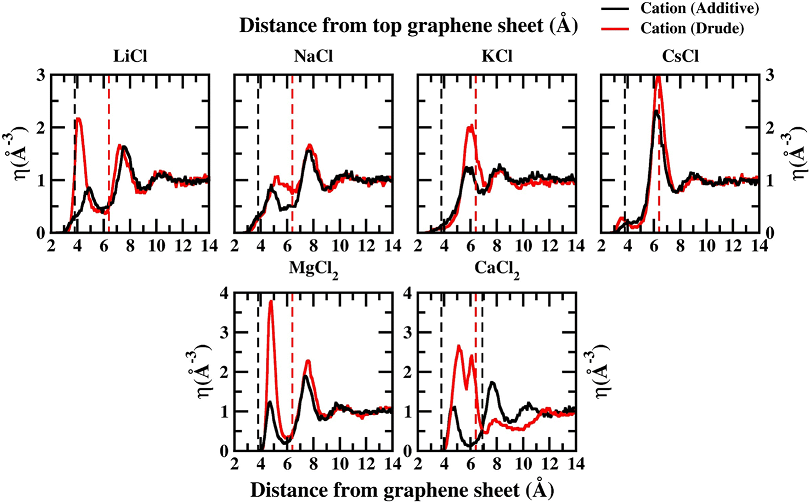
\includegraphics[width=\textwidth]{Chapter3/Figures/Figure4.png}
    \caption[Density profiles for all ions calculated from additive and Drude polarizable FF simulations of 1 M salt solutions. Location of the peak corresponding to the Cl\textsuperscript{-} ion density is depicted using dashed lines]{Density profiles for all ions calculated from additive (black) and Drude polarizable (red) FF simulations of 1 M salt solutions. In each panel we also present the location of the peak corresponding to the Cl\textsuperscript{-} ion density using dashed lines. All densities are presented in units of $\angstrom^{-3}$ and all distances are presented in units of $\angstrom$.}
\end{figure}

\begin{figure}
    \centering
    \includegraphics[width=\textwidth]{Chapter3/Figures/Figure5.png}
    \caption[Number density ($\eta$) for water molecules as a function of the distance from topmost graphene sheet, from 1M additive and Drude polarizable FF salt simulations]{Number density ($\eta$) for water molecules as a function of the distance from topmost graphene sheet, from 1M additive and Drude polarizable FF salt simulations. All distances are presented in units of $\angstrom$.}
\end{figure}

In order to capture the influence of the FF on interfacial dynamics in a realistic system we study the dynamics of 1 M salt solutions of LiCl, NaCl, KCl, CsCl, MgCl\textsubscript{2} and CaCl\textsubscript{2}. A representative image depicting the system setup is presented in Figure 5.1(c). We compute the density profiles of the ions as a function of the distance from the topmost graphene surface to establish the effect of polarization on the ion - graphene interactions. The density profiles obtained from additive and Drude polarizable FF simulations are presented in Figure 5.4. Before commenting on the distribution of the cations we analyse the distribution of the water and the counter-ion Cl\textsuperscript{-} in these simulations. The distribution of the water molecules as a function of distance from the topmost graphene sheet for all the systems is presented in Figure 5.5.  For all the systems, we observe a bimodal distribution with peaks at 3.30 $\angstrom$ and 6.10 $\angstrom$ for the TIP3P additive water model and at 3.40 $\angstrom$ and 6.20 $\angstrom$ for the SWM4 Drude polarizable water model.  The first peak corresponds to the direct interaction of the water molecules with the graphene sheet. In Figure 5.6 we present the distribution of the counterion Cl\textsuperscript{-} as a function of the distance from the topmost graphene surface for all the systems. In the additive simulations we observe a significant peak at around 6.40 $\angstrom$ for all the systems. This peak is indicative of fully solvated Cl\textsuperscript{-} ions interacting with the graphene surface in the additive simulations. For the Drude polarizable simulations we observe a significant peak at around 3.80 $\angstrom$ which implies a direct interaction between the Cl\textsuperscript{-} ions and the graphene surface. These observations are directly related to the underlying free energy distribution, wherein the free energy minimum is observed at around 6.10 $\angstrom$ for the additive FF and around 3.90 $\angstrom$ for the Drude polarizable FF [Figure 5.3]. For the Drude polarizable simulations we also observe a dependence on the cations from the peak height of the distribution at 3.80 $\angstrom$. The height of the peak follows the trend Ca\textsuperscript{2+} > Mg\textsuperscript{2+} > Li\textsuperscript{+} $\approx$ Na\textsuperscript{+} > K\textsuperscript{+} > Cs\textsuperscript{+}. For Ca\textsuperscript{2+} we also observe a strong bimodal distribution of the Cl\textsuperscript{-} ions with a second significant peak at 6.80 $\angstrom$.

\begin{figure}
    \centering
    \includegraphics[width=\textwidth]{Chapter3/Figures/Figure6.png}
    \caption[Number density ($\eta$) for Cl\textsuperscript{-} as a function of the distance from topmost graphene sheet, from 1M additive and Drude polarizable FF salt simulations]{Number density ($\eta$) for  Cl\textsuperscript{-} as a function of the distance from topmost graphene sheet, from 1M additive and Drude polarizable FF salt simulations. All distances are presented in units of $\angstrom$.}
\end{figure}

The ion density distribution for the cations depends on both the size of the cation as well as the underlying FF. For all the systems we observe that the additive simulations favour the interactions between the solvated cation and the graphene sheet, with the major peak in the distribution being observed in the range between 5.7-7.7 $\angstrom$. We observe that this is being driven by the distribution of the counter ion Cl\textsuperscript{-} in the system which is observed at around $\approx$6.40 $\angstrom$ for all the systems. For Li\textsuperscript{+}, Na\textsuperscript{+}, Mg\textsuperscript{2+} and Ca\textsuperscript{2+} we also observe minor peaks in the distribution at 4.9 $\angstrom$, 4.8 $\angstrom$, 4.8 $\angstrom$ and 4.7 $\angstrom$, which correspond to the direct interaction of the ions with the graphene surface or the interaction of a partially solvated ion with the graphene surface. For Li\textsuperscript{+}, Na\textsuperscript{+}, Mg\textsuperscript{2+} and Ca\textsuperscript{2+} this interaction is favoured due to the favourable free energy associated with such interactions [Figure 5.2] in the additive FF. For the Drude polarizable FF we observe two distinct favourable interactions depending on the cations. Li\textsuperscript{+}, Mg\textsuperscript{2+} and Ca\textsuperscript{2+} favour a direct interaction between the cations or partially solvated cations and the graphene surface with the major peak in the distribution being observed at 4.0 $\angstrom$, 4.8 $\angstrom$ and 5.1 $\angstrom$, respectively. On the other hand, Na\textsuperscript{+}, K\textsuperscript{+} and Cs\textsuperscript{+} favour interaction between a fully solvated cation and the graphene surface, with the major peaks being observed at 7.7 $\angstrom$, 6.1 $\angstrom$ and 6.4 $\angstrom$ respectively. Interestingly for Ca\textsuperscript{2+} we observe the next peak in the distribution at 6.1 $\angstrom$. This close pacing of the peaks is correlated to the broad shallow minimum observed in the free energy profile for Ca\textsuperscript{2+} obtained using the Drude polarizable FF parameters [Figure 5.3]. The increased propensity of Li\textsuperscript{+}, Mg\textsuperscript{2+} and Ca\textsuperscript{2+} to reside close to the graphene surface in Drude polarizable FF simulations is also driven by the prominent density of Cl\textsuperscript{-} near the graphene surface with the Cl\textsuperscript{-} distribution being observed at 3.8 $\angstrom$. A decrease in the Cl\textsuperscript{-} ion density at 3.8 $\angstrom$, which is correlated to the peak height at 3.8 $\angstrom$ (Ca\textsuperscript{2+} > Mg\textsuperscript{2+} > Li\textsuperscript{+} $\approx$ Na\textsuperscript{+} > K\textsuperscript{+} > Cs\textsuperscript{+}) results in a shift in the Na\textsuperscript{+}, K\textsuperscript{+} and Cs\textsuperscript{+} densities away from the graphene surface.

\begin{figure}
    \centering
    \includegraphics[width=\textwidth]{Chapter3/Figures/Figure7.png}
    \caption[First hydration number ($\eta_1$) for Li\textsuperscript{+}, Na\textsuperscript{+}, K\textsuperscript{+}, Cs\textsuperscript{+}, Mg\textsuperscript{2+}, Ca\textsuperscript{2+} and Cl\textsuperscript{-} ions from 1 M ion - graphene simulations as a function of distance from the graphene surface. Average dipole moment ($\mu$) for water molecules in various 1 M salt solutions discussed in the study are also presented]{(a) First hydration number ($\eta_1$) for Li\textsuperscript{+}, Na\textsuperscript{+}, K\textsuperscript{+}, Cs\textsuperscript{+}, Mg\textsuperscript{2+}, Ca\textsuperscript{2+} and Cl\textsuperscript{-} ions from 1 M ion - graphene simulations as a function of distance from the graphene surface. (b) Average dipole moment ($\mu$) for water molecules in various 1 M salt solutions discussed in the study. All distances are presented in units of $\angstrom$. Dipole moments are presented in units of Debye.}
\end{figure}

Before concluding we analyse the hydration dynamics of the water molecules around the ions from the Drude polarizable FF simulations. In Figure 5.7(a) we present the average hydration number computed for ions within blocks of 1 A as a function of distance from the graphene sheet. For the monovalent ions we observe that the hydration number increases as a function of the size of the ion. The average hydration number for Li\textsuperscript{+} and Na\textsuperscript{+} was found to be 3.96 and 5.62 irrespective of the distance from the graphene sheet indicative of a near tetra-coordinated and near hexa-coordinated structure for the first hydration shell in these systems. This is also observed in the representative structures presented in Figure 5.2. The larger monovalent ions K\textsuperscript{+} and Cs\textsuperscript{+} exhibit variable hydration numbers depending upon the distance from the graphene sheet. The K\textsuperscript{+} ions exhibit a distorted pentagonal bipyramidal geometry in the bulk with the hydration number being 6.92 for the first hydration shell. Closer to the graphene sheet the hydration number is found to be 5.25 indicating a loss of one/two water molecules from the bulk hepta-coordinated structure. For the largest ion Cs\textsuperscript{+} we observe variable hydration numbers in the bulk, with the hydration number varying from 9.21 to 11.05. This indicates an unstructured dynamic first hydration shell around Cs\textsuperscript{+}. Close to the graphene surface the hydration shell easily loses water molecules and the hydration number drops to 8.21. For the divalent ion Mg\textsuperscript{2+} the average hydration number was found to be 6.00 irrespective of the distance from the graphene sheet. However, a closer inspection of the structure of the hydration shell reveals that near the graphene sheet the hydration shell rearranges into a pentagonal pyramidal structure while in the bulk the hydration shell resembles an octahedral structure [Figure 5.3]. The larger divalent ion Ca\textsuperscript{2+} exhibits a variable hydration number like K\textsuperscript{+} and Cs\textsuperscript{+}. Close to the graphene sheet the hydration number is found to be 3.18, while in the bulk solution the hydration number was found to vary between 3.00 and 4.65. This points to a significant deviation from the octa-coordinated crystal environment for the Ca\textsuperscript{2+} ions in CaCl\textsubscript{2} salt. The hydration shell around Cl\textsuperscript{-} also undergoes partial reorganization upon interacting with the graphene surface. The hydration number drops to 6.02 from a bulk value of 6.65. Visualizing the hydration shell structure reveals a pentagonal pyramidal arrangement of water molecules around Cl\textsuperscript{-} similar to the arrangement observed for Mg\textsuperscript{2+} [Figure 5.3].

Finally, we analyse the dipole moment of the water molecules as a function of the distance from the graphene surface. In Figure 5.7(b) we present the average dipole moment computed for water molecules within blocks of 0.5 $\angstrom$ as a function of distance from the graphene sheet. We note that, from additive FF simulations, the dipole moment of water molecules is constrained to be 2.374 D due to the rigid water model used in the simulations. However, the SWM4 water model used in the Drude polarizable FF simulations is able to respond to the changes in the local environment. Very close to the graphene sheet the average dipole moment of water molecules stabilizes at around 2.41 D, wherein the water molecules are in close contact with the hydrophobic graphene and the influence of ions is not felt. Moving away from the graphene sheet we begin to observe an increase in the ion densities of both the anions and the cations [Figure 5.4]. For MgCl\textsubscript{2} and LiCl simulations, we observe a significant change in the average dipole moment of water with the dipole moment increasing to 2.58 D and 2.51 D at a distance of 5.7 $\angstrom$ from the graphene sheet. This is due to the small size of Mg\textsuperscript{2+} (0.70 $\angstrom$) and Li\textsuperscript{+} (0.71 $\angstrom$) ions, which favours a large charge/surface area ratio resulting in significant polarization of the local environment. On the other hand, for the larger cations we observe a reduced impact of the ions on the average dipole moment of water.

To comment on ion - graphene interactions and how the charges on the ions and the graphene surface respond to such interactions we analyse the dipole moment fluctuations for both the ions and the interacting graphene surface. In Figure C.1 of the Appendix C we present the instantaneous dipole moment of the ions as a function of distance from the graphene surface. In Figure C.2 of the Appendix C we present the instantaneous dipole moment of the interacting graphene surface as a function of distance from the ions. The instantaneous dipole moments of the ions [Figure C.1] and interacting graphene surface [Figure C.2] are found to be invariant with respect to the distance between the ions and the graphene surface. This indicates an absence of direct interaction between the ions and the graphene surface. This is highlighted in the observed distribution of the instantaneous dipole moment of the graphene sheet [Figure C.2], which appears independent of the chemical nature of the ions. However for both the ions and the graphene sheet we observe a spread in the dipole distribution. For the ions [Figure C.1] we observe a strong correlation between the distribution of the instantaneous dipole moments and the charge to surface ratio of the ions, with small ions such as Li\textsuperscript{+} and Mg\textsuperscript{2+} exhibiting a very small dipole distribution and larger ions such as Cs\textsuperscript{+} and Ca\textsuperscript{2+} exhibiting a broader distribution. This distribution can be traced back to the ion - water interactions in the first solvation shell of the ions. For the graphene sheet we observe a distribution from 0.0 D to 2.4 D [Figure C.2]. This dipole response of the graphene surface can be traced back to the interactions with the water molecules present in the 1\textsuperscript{st} monolayer of water observed at 3.40 $\angstrom$ [Figure 5.5]. Thus, we only observe solvent driven interactions between the ions and the graphene surface.
\section{Conclusions}
In conclusion, we show that the Drude polarizable FF parameters for graphene\supercite{h_polarization_2021} along with the parameters for ions\supercite{yu_simulating_2010} reliably capture the dynamics at the graphene electrolyte interface. The Drude parameters are able to capture both the size and charge dependent ion - graphene interactions, which cannot be captured by additive simulations. In particular the Drude parameters are able to capture the anion - graphene interactions, which are severely underestimated in the additive simulations. Additionally, the Drude polarizable simulations also capture the influence of ions on solvation dynamics. These results establish the applicability of Drude parameters for studying ion - graphene interface interactions, like those observed in graphene-based membranes for desalination,\supercite{sun_selective_2014,joshi_precise_2014,homaeigohar_graphene_2017,boretti_outlook_2018,yang_ultrathin_2017} or graphene-based electrodes in energy storage.\supercite{liang_graphene-based_2009,wang_supercapacitor_2009,wang_sngraphene_2009,stoller_graphene-based_2008} The Drude parameters also present an effective alternative to computationally expensive first-principles MD simulations.
    \chapter[Unveiling DNA Translocation in Pristine Graphene Nanopores: Understanding Pore Clogging via Polarizable Simulations]{Unveiling DNA Translocation in Pristine Graphene Nanopores: Understanding Pore Clogging via Polarizable Simulations \protect\footnote[5]{This chapter has been published as \textbf{H., Hemanth} and Mallajosyula*, S.S.; Unveiling DNA Translocation in Pristine Graphene Nanopores: Understanding Pore Clogging via Polarizable Simulations; {\textit{ACS Appl. Mater. Interfaces}, 2023, \textbf{47}, 55095–55108}}}

\section[Introduction]{Introduction}
Whole genome sequencing (WGS) is recognized as a key step in the advancement of modern medicine, with major implications in the development of personalized treatment protocols.\supercite{dewey_clinical_2014} WGS would enable the early identification of genetic disorders and would help in providing suitable medical attention to the general public.\supercite{abubaker_bagabir_covid-19_2022} In the recent years, the importance of WGS was highlighted in tracking the spread of novel coronavirus (Covid-19) and the subsequent development of suitable vaccines to curb the spread of the infection.\supercite{chen_next-generation_2021} WGS enabled the identification of the variants of concern of the severe acute respiratory syndrome coronavirus 2 (SARS-CoV-2) as the virus mutated, which greatly influenced the policy response towards the pandemic situation.\supercite{abubaker_bagabir_covid-19_2022,chen_next-generation_2021} Key to WGS is the requirement of a rapid, accurate and cost-effective sequencing platform.\supercite{giani_long_2020} Traditional efforts on sequencing the DNA are based on the Sanger method, where the DNA strand of interest is fragmented, and amplified before being sequenced.\supercite{sanger_dna_1977} The sequence of the original DNA strand is then recovered based on the overlaps in the fragmented DNA. The traditional sanger-based methods are time-consuming and laborious which lead to the development of next generation sequencing (NGS) technologies that use massively parallel sequencing approaches.\supercite{manyana_hiv-1_2021} However even the NGS methods rely on the fragmentation of the original DNA strand.

Nanopores offer an alternative platform for DNA sequencing that does not involve strand fragmentation. The basic principle of nanopore sequencing is that the analytes enter the nanopore under an applied potential which alters the flow of ions through the nanopore resulting in blockades of the ionic current.  These resultant ionic current blockades are analysed to identify the analyte. Two variants of nanopores have been explored for DNA sequencing (i) Biological nanopores and (ii) Solid state nanopores. Biological nanopores are formed by the self-assembly of protein, peptides or even DNA scaffolds in lipid bilayers or polymer membranes and have been successfully used in sequencing technology.\supercite{hu_biological_2021} However, one of the key limitations of biological nanopores is that they are very susceptible to changes in pH and temperature and cannot be readily reused, which affects their scope of application.\supercite{haque_solid-state_2013} Solid state nanopores, on the other hand provide a stable alternative to the biological nanopores. Solid state nanopores are typically fabricated using techniques like electron milling,\supercite{storm_fabrication_2003} laser-based etching\supercite{gilboa_optically-monitored_2018} and dielectric breakdown of solid membranes,\supercite{waugh_solid-state_2020} which allows one to control the dimensions of the nanopore. Initial studies using conventional silicon based nanopores were not successful in DNA sequencing due to the relatively large thickness of the nanopore membrane that corresponded to multiple nucleobases occupying the nanopore at the same time leading to a loss of resolution.\supercite{li_dna_2003} This led to the search for substrates with thickness that would allow single nucleobases to occupy the nanopore while translocating through it. 

The discovery of graphene\supercite{geim_graphene_2009} and related 2D materials\supercite{novoselov_two-dimensional_2005} of sub nanometre thickness ignited the possibility of using such materials as suitable membranes for DNA sequencing. These 2D membranes in principle address the challenges of stability associated with biological nanopores\supercite{mayer_biological_2022} and membrane thickness associated with silicon based solid state nanopores.\supercite{li_dna_2003} In 2010 a series of initial experiments demonstrated the detection of DNA passing through graphene nanopores.\supercite{schneider_dna_2010,merchant_dna_2010,garaj_graphene_2010} These experiments led to numerous other studies exploring 2D materials for DNA sequencing technologies. We refer the readers to excellent review articles which summarize the progress made in DNA sequencing using graphene and other 2D materials.\supercite{xue_solid-state_2020,qiu_nanopores_2021} Despite the initial excitement the key aim of achieving single-base resolution using graphene nanopores has remained elusive. One of the major issues has been the translocation dynamics of DNA in the nanopore.\supercite{venkatesan_nanopore_2011} Translocation speeds of 20,000-100,000 basepairs/ms have been observed in typical graphene based nanopore experiments. These speeds are generally observed due to the very large pore diameters (3-25 nm)\supercite{schneider_dna_2010,merchant_dna_2010,garaj_graphene_2010} and contaminated graphene lattices used in these studies. On the other hand, Dekker and co-workers reported that clean crystalline graphene nanopores are prone to severe clogging and pore closures for pore diameters ranging from 3 nm to 20 nm.\supercite{schneider_tailoring_2013} These crystalline graphene pore diameters are ideal for observing translocation speeds of 1-100 basepairs/ms which are ideal for achieving single base detection. Understanding the atomistic interactions responsible for the pore clogging and translation dynamics would provide insight into the future development of graphene based nanopores.

Molecular dynamics (MD) simulations studying the translocation dynamics of both single-stranded DNA (ssDNA) and double-stranded DNA (dsDNA) in graphene nanopores have provided atomistic level insights into the translocation events.\supercite{barati_farimani_dna_2017} In a seminal work Aksimentiev and co-workers used MD simulations to address the suitability of graphene nanopores for sequencing ssDNA.\supercite{wells_assessing_2012} In their simulations and in most MD simulations subsequently the graphene nanopore is represented as a clean crystallographic nanopore with the graphene lattice being preserved up to the edges of the nanopore. Aksimentiev and co-workers observed that ssDNA was found to adhere to the graphene surface resulting in 2D diffusion of the adhered DNA on the graphene surface, limited translocation events and even clogging of the pore that required transmembrane bias of about 500 mV to unclog and complete the translocation event. In some cases, the bias voltage had to be increased to 800 mV to complete the translocation event. The pore diameter for which translocation events were observed was 16 Å. Many of these observations were later corroborated in the experimental study by Dekker and co-workers.\supercite{schneider_tailoring_2013,heerema_graphene_2016} However one significant difference between the two studies was the severity of the pore clogging in the experimental study which was not captured in the MD simulations. Using a pore diameter of 50 Å, which was significantly larger than the 16 Å diameter used in the MD studies, Dekker and co-workers observed significant pore clogging which could not be relieved even under the application of multiple large 1V pulses.\supercite{schneider_tailoring_2013} In the MD simulations ramping up the bias by 300 mV was sufficient to progress the translocation event. Subsequent MD studies have also reported a smooth translocation of DNA strands via the nanopores under the application of a bias voltage.\supercite{tyagi_revealing_2019} We note that all these simulations were performed using the additive (non-polarizable) force-fields (FF), which do not account for charge transfer and polarization effects due to the fixed-point charges associated with the atoms in the additive (non-polarizable) FF. This becomes especially crucial when trying to describe the large $\pi$-cloud above the graphene surface. A way to address this issue is the inclusion of polarization into MD simulations. 

The importance of polarizable description of surfaces, especially treating the induced charges in the presence of solvent and counter ions has been recognized when describing interfacial phenomenon\supercite{kondrat_theory_2023,siepmann_influence_1995}. The Drude model presents a simple extension of the potential which can be easily implemented and remains compatible with common bio-molecular force fields, as described by the implementation of the Drude model potential for metallic surfaces.\supercite{geada_insight_2018} Drude parameters have also been developed to describe graphene surfaces.\supercite{ho_polarizability_2013,misra_insights_2017} Striolo et. al. targeted the per atom polarizability of 0.867 Å\textsuperscript{3} for graphene C atoms based on ab-initio calculations of the out-of-plane polarization of multi-layer graphene in vacuum and did not include solvation effects.\supercite{ho_polarizability_2013} In an unrelated study Blanksctein et. al. used a site polarizability of 1.139 and a thole scaling factor of 1.507 to describe the graphene C atoms to capture the wetting of the graphene surfaces by water and reproduce experimentally observed contact angles.\supercite{misra_insights_2017} These Drude parameters were not tested to study $\pi$-$\pi$ interactions between graphene surfaces and aromatics. Towards this endeavour we reported the development of Drude parameters for describing a polarizable graphene sheet which remains compatible with the existing parameters in the CHARMM Drude polarizable force field that encompasses proteins, nucleic acids, carbohydrates and small molecules.\supercite{h_polarization_2021} We used a site polarizability of 1.615 and a thole scaling factor of 1.195 to describe the C atoms in the graphene sheet. These parameters are consistent with the description of aromatics in the CHARMM Drude polarizable force field.\supercite{lopes_polarizable_2007} The parameters were tested to reproduced water-binding energies and nucleobase-graphene $\pi$-$\pi$ interaction energies. The developed parameters were first used to study the aggregation behavior of nucleobases dispersed on a graphene support.\supercite{h_polarization_2021} The polarizable simulations were able to capture experimentally observed $\pi$-$\pi$ stacking interactions amongst Guanine nucleobases\supercite{varghese_binding_2009} and the formation of ordered self-assemblies for Adenine and Cytosine nucleobases.\supercite{otero_elementary_2008,wandlowski_structure_1996} The parameters were also used to study the concentration dependent self-assembly of cytosine nucleobases on 2D graphene support.\supercite{h_capturing_2022} Wherein, in the low surface loading concentration (0.25 M) limit the simulations were able to capture ordered self-assemblies that were consistent with the experimental assemblies of cytosine nucleobases adsorbed on 1-octanol/HOPG solid-liquid interfaces\supercite{xu_coadsorption_2006} and Au(111) surfaces\supercite{otero_elementary_2008,wandlowski_structure_1996} observed via HR-STM-imaging. Additionally, the developed parameters were also used to capture the solvation dynamics of ions at the graphene electrolyte interface.\supercite{h_capturing_2023} The polarizable simulations were able to capture both the size and charge dependent ion-graphene interactions. In particular, the Drude parameters were able to reliably capture the anion-graphene interactions. We note that all these effects which were captured by polarizable simulations are severely underestimated in the additive (non-polarizable) simulations.\supercite{h_polarization_2021,h_capturing_2022,h_capturing_2023} Polarizable force fields have also been found to accurately describe the thermodynamics of ion permeation in biological nanopores which could not be described by additive (non-polarizable) simulations.\supercite{prajapati_computational_2020} In this study, we use polarizable simulations for the first time to study the translocation dynamics of ssDNA through a graphene nanopore. 

\section{Computational Methodology}
We constructed four single stranded DNAs (ssDNA), as twenty nucleoside homopolymers of deoxy-adenosine (dA\textsubscript{20}), deoxy-guanosine (dG\textsubscript{20}), deoxy-cytidine (d\textsubscript{20}) and deoxy-thymidine (dT\textsubscript{20}) using the topology information present in the Chemistry at HARvard Molecular Mechanics (CHARMM) nucleic acid force field.\supercite{hart_optimization_2012,foloppe_all-atom_2000,mackerell_all-atom_2000} A multilayer graphene, consisting of three graphene sheets in ‘A-B-A’ arrangement was constructed using Inorganic Builder plugin available in VMD.\supercite{humphrey_vmd_1996} A nanopore of radius 8 Å was constructed in the nanopore by removing the atoms within 8 angstroms of the center-of-mass (COM) of each graphene layer. Dangling bonds (bonds with unsatisfied valences) were manually identified and removed during the construction of the nanopore. Aksimentiev and co-workers investigated a series of pore geometries and observed that the step wise translocation was observed for a pore diameter of 16 Å in a 3-layer graphene system.\supercite{wells_assessing_2012} Thus, the pore radius of 8 Å was considered to remain consistent with the study by Aksimentiev and co-workers and to facilitate a direct comparison with the previous study.\supercite{wells_assessing_2012} We chose to leave the pore edges unsaturated to remain consistent with the previous study.\supercite{wells_assessing_2012} The ssDNA strand was oriented along the z-axis, with three nucleotides at the 5’-end of the strand threaded through the nanopore, to minimize the onset of translocations. The combined ssDNA-multilayer graphene system was solvated and neutralized with 1M KCl using solvate and Autoionize plugins in VMD. Representative structure depicting the system setup is presented in Figure 6.1. CHARMM36 all-atom FF was used to describe bonded and non-bonded interactions in ssDNA,\supercite{hart_optimization_2012,foloppe_all-atom_2000,mackerell_all-atom_2000} ions\supercite{beglov_finite_1994} and the multilayer graphene.\supercite{vanommeslaeghe_charmm_2009} TIP3P three-point water model\supercite{jorgensen_comparison_1983} was employed to describe water molecules in additive (non-polarizable) FF simulations. 
\begin{figure}
    \centering
    \includegraphics[width=\textwidth]{Chapter4/Figures/Figure1.png}
    \caption[Representative structures depicting the system setup for ssDNA – multilayer graphene.]{Representative structures depicting the system setup for ssDNA – multilayer graphene. (a) Side View and (b) Oblique view of the multilayer graphene to indicate periodic boundary conditions employed. (c) Complete ssDNA – multilayer graphene (water molecules are removed for clarity). All figures are prepared using VMD.\supercite{humphrey_vmd_1996}}
\end{figure}

For the polarizable simulations we employed in-house scripts to add Drude particles to the additive (non-polarizable) FF systems and generate corresponding Drude polarizable systems. Drude polarizable FF was used to describe the bonded and non-bonded interactions in ssDNA\supercite{baker_development_2011,savelyev_all-atom_2014} and ions.\supercite{lin_polarizable_2018} Parameters previously reported by us were used to describe bonded and non-bonded interactions in the multilayer graphene.\supercite{h_polarization_2021} SWM4-NDP four-point polarizable water model was used to describe the water molecules.\supercite{lamoureux_polarizable_2006} We restrained the bond lengths and bond angles in water molecules using the SETTLE\supercite{miyamoto_settle_1992} algorithm in Drude polarizable FF simulations.

All-atom MD simulations were performed using the Nanoscale Molecular Dynamics (NAMD) package.\supercite{phillips_scalable_2005} We employed a real-space cut-off of 9 Å while evaluating electrostatic interactions using Particle Mesh Ewald\supercite{darden_particle_1993} (PME) summation. Equations of motion were integrated using a time step of 1 fs for additive (non-polarizable) FF simulations and a reduced time step of 0.5 fs for Drude polarizable FF simulations. We employed a Langevin thermostat to maintain the simulated system at 298 K. An additional dual thermostat was employed to couple the Drude particles to an ice-bath at 1K. Systems were minimized for 40,000 conjugate-gradient steps to remove unfavorable contacts. The minimized geometries were further equilibrated for 2 ns in an isothermal-isobaric (NPT) ensemble followed by 3 ns in an isothermal-isochoric (NVT) ensemble.  Production runs in an isobaric-isochoric (NVT) ensemble were performed for 500 ns or till a complete translocation of the ssDNA in the additive (non-polarizable) simulations, for Drude the simulations were run for 200 ns or till a complete translocation of the ssDNA is observed. 

For the additive (non-polarizable) FF simulations, the initial applied external bias was set to 0.50 V (500 mV) for the first 100 ns of the production runs. The external bias was then increased to 0.75 V (750 mV) for the next 150 ns in the production runs. Subsequently the external biases were increased to 1.00 V, in an attempt to drive the translocation to completion. 

For the Drude polarizable FF two initial independent runs were initiated with bias voltages of 0.5 V and 1.0 V for 50 ns and 100 ns respectively. No translocations were observed during the 0.5 V runs and for the 1.0 V runs translocations were observed only for dT\textsubscript{20}. Based on these observations for effecting translocations, the initial applied external bias was set to 1.0 V for the first 20 ns of the production runs. The bias was ramped up to 1.50 V for the next 80 ns. After the completion of 100 ns the applied external bias was increased to 1.75 V in an attempt to drive the complete translocation. 

To understand the energetics of the DNA graphene interactions we also computed binding free energies corresponding to the nucleoside-graphene and the modified-nucleotide-graphene interactions using adaptive biasing force (ABF) simulations. We use a modified nucleotide (nucleotide') with phosphate at the 3’ and 5’-ends passivated by methyl groups. This was to mimic the sugar phosphate backbone and the charges observed in the single strand DNA. ABF simulations were also used to compute binding free energies of deoxy-ribose graphene interactions and dimethyl phosphate graphene interactions. For the ABF simulations, the systems were setup as a four-layered graphene block in a ‘ABAB’ stacking arrangement. The methodology for computing the binding free energies from ABF simulations were adopted from the previous work by Comer et. al, where four-layered graphene sheets were employed as a template for multi-layer graphene.\supercite{comer_predicting_2015} The initial coordinates of the nucleosides, nucleotides, deoxy-ribose sugar and dimethyl phosphate were constructed using the topology information available in the CHARMM additive (non-polarizable) FF.\supercite{hart_optimization_2012,foloppe_all-atom_2000,mackerell_all-atom_2000} In-house scripts were used to add the Drude particles to prepare the files for Drude polarizable simulations. We present a representative structure depicting the system setup in Figure 6.2. 
\begin{figure}
    \centering
    \includegraphics[width=\textwidth]{Chapter4/Figures/Figure2.png}
    \caption[Representative structures depicting the scan coordinate employed in adaptive biasing force (ABF) simulations of adenosine and dimethyl phosphate molecules]{Representative structures depicting the scan coordinate employed in adaptive biasing force (ABF) simulations of (a) adenosine molecule and (b) dimethyl phosphate molecule}
\end{figure}

To establish the inherent secondary structural preferences of ssDNA we simulated freestanding ssDNA also. Freestanding ssDNA structures were solvated in an orthorhombic box of dimensions 80 x 80 x 120 Å\textsuperscript{3}. KCl ions were added to the system using the AutoIonize plugin in VMD to bring the system to 1M concentration. The structures were minimized for 40,000 conjugate-gradient steps. The minimized structures were subsequently equilibrated for a total of 5 ns in NPT and NVT ensembles. Corresponding Drude polarizable FF input files were generated using ‘DrudePrepper’ functionality in CHARMM-GUI web interface\supercite{kognole_charmmgui_2022} using the equilibrated structures. Production runs for 100 ns using the additive (non-polarizable) and Drude polarizable FF were performed using the OpenMM simulation package\supercite{eastman_openmm_2017} in an NPT isobaric-isothermal ensemble. A timestep of 1 fs was employed for integrating the equations of motion in both the additive (non-polarizable) and Drude polarizable FF simulations. Translocation of ssDNA through the nanopores were tracked using in-house scripts, following the methodology described by Wells et. al.\supercite{wells_assessing_2012}  Relative orientation and the dipole moment analysis for the nucleotides were performed using in-house codes.

\section[Results and Discussions]{Results and Discussions}
\subsection[Additive (Non-Polarizable) Simulations]{Additive (Non-Polarizable) Simulations}
Before presenting the results from the Drude polarizable simulations we first present the results from the additive (non-polarizable) simulations to establish a point of comparison. In Figure 6.3(a) we illustrate the timeseries of the translocation events observed in the additive (non-polarizable) simulations. A nucleobase is recorded as a translocated nucleobase once the z-coordinate of the center of mass of the nucleobase is greater than the z-coordinate of the center of mass of the bottom graphene sheet. This metric also allows us to capture the exit and opposite re-entry of the translocated nucleobases. As mentioned in the methods section, for the additive (non-polarizable) FF simulations the applied external bias was set to 0.50 V for the first 100 ns. This was then increased to 0.75 V for the next 150 ns and subsequently ramped up to 1.00 V in an attempt to drive the translocation to completion. In the additive (non-polarizable) simulations, the 3’-end of the ssDNA was found to adhere quickly onto the graphene surface within the first $\approx$20 ns for the pyrimidine strands dC\textsubscript{20} and dT\textsubscript{20}, while for the purine strands dA\textsubscript{20} and dG\textsubscript{20} the same was observed within the first $\approx$45 ns. In Figure D.1 of the Appendix D we present the z-coordinate projection of the center of mass of the 3’-end nucleobases (18, 19 and 20) with respect to the top layer graphene sheet, to allude to this observation. The bases adhere onto the graphene surface via $\pi$-$\pi$ interactions between the nucleobases and the graphene surface. For the pyrimidine strands dC\textsubscript{20} and dT\textsubscript{20} we observe rapid translocation of the first 6 and 5 nucleobases respectively, within the first 20 ns of the simulations while the 3’-end of the ssDNA adheres to the graphene surface. In Figure 6.3(b) we present a representative snapshot of dC\textsubscript{20} recorded at 20ns to illustrate the adhering of the 3’-end of the ssDNA to the graphene surface. We observe that the translocated nucleobases remain adhered to the bottom graphene sheet. Following this initial rapid translocation, for dC\textsubscript{20} we observe pore blockage till 100 ns with nucleobase 7 and 8 getting stuck in the nanopore. During this period, we observe multiple exit and re-entry events of nucleobase 7 into the nanopore. During this 80 ns window the complete ssDNA strand adheres itself to the top graphene surface and undergoes 2D diffusion. In Figure 6.3(c) we present a representative snapshot of dC\textsubscript{20} recorded at 100ns to illustrate this observation. This behavior is observed for both the purine and pyrimidine strands, wherein after the initial adsorption of the 3’end nucleobases onto the graphene sheet the remaining nucleobases also get adsorbed onto the graphene surface and undergo 2D diffusion. For dT\textsubscript{20} we observe a sequential stepwise translocation of the first 11 nucleobases till 100 ns. Amongst the purine strands for dA\textsubscript{20} we did not observe any translocation events in the first 100 ns, with nucleobase 3 exiting and re-entering the nanopore. For dG\textsubscript{20} we observe a spontaneous translocation of 6 nucleobases in the first 45 ns which also corresponds to the time taken for the 3’-end of the ssDNA to adheres to the graphene surface. Once the 3’-end of dG\textsubscript{20} adheres to the graphene surface we observe only lateral diffusion of the ssDNA and no further translocation. Thus, within the first 100 ns the complete ssDNA strand adheres to the graphene sheet on either side of the nanopore and the resultant translocation is driven by the ionic current and the applied bias.
\begin{figure}
    \centering
    \includegraphics[width=\textwidth]{Chapter4/Figures/Figure3.png}
    \caption[DNA translocation through nanopores in a three-layer graphene membrane in additive FF]{DNA translocation through nanopores in a three-layer graphene membrane. (a) Number of translocated nucleobases as a function of simulation time obtained from additive (non-polarizable) simulations. Vertical dotted lines indicate change in the applied bias potential. (b) Representative snapshot of dC\textsubscript{20} recorded at 20 ns indicating the adhering of the 3’ end of the ssDNA onto the graphene surface. (c) Representative snapshot of dC\textsubscript{20} recorded at 100 ns indicating the adhering of the complete ssDNA onto the graphene surface. All nucleobases adhering to the top-graphene sheet are presented in orange, while those adhering to the bottom-graphene sheet are presented in green. (d) Representative snapshot of translocated dG\textsubscript{20} ss DNA.}
\end{figure}

To complete the translocation of the strands we increase the bias to 1.0 V. The increased bias resulted in a rapid step wise translocation of pyrimidine dC\textsubscript{20} within 280 ns. For the purine strands the higher bias restarts the translocation with stepwise nucleobase exits being observed between 340 ns and 410 ns for dA\textsubscript{20}, which is followed by a rapid exit from the nanopore with the last 6 nucleobases exiting within 5 ns. For dG\textsubscript{20} the increased bias relieves the pore clogging and translocation events are observed with nucleobases 8, 9, 10 translocating the nanopore. This is followed by a brief clogging period wherein nucleobases 10 and 11 remain trapped in the nanopore. However, once nucleobase 11 leaves the pore the remaining 9 nucleobases translocate within 5 ns, due to the significantly large bias. In Figure 6.3(d) we present a representative snapshot to illustrate the complete translocation of dG\textsubscript{20}. Following the translocation, the strand undergoes 2D diffusion on the graphene surface. 

\subsection{Drude Polarizable Simulations}
\begin{figure}
    \centering
    \includegraphics[width=\textwidth]{Chapter4/Figures/Figure12.png}
    \caption[Number of translocated nucleobases as a function of simulation time obtained from (a) 0.5 V and (b) 1.0 V Drude polarizable simulations.]{Number of translocated nucleobases as a function of simulation time obtained from (a) 0.5 V and (b) 1.0 V Drude polarizable simulations.}
\end{figure}

For the Drude simulations we did not observe any translocations for a bias voltage of 0.5 V. Translocations were observed only for dT\textsubscript{20} when the bias voltage was increased to 1.0 V. In Figure 6.4 we present the time series corresponding to simulations performed at 0.5 V and 1.0 V to illustrate our observations. Thus, in order to study the translocations of ssDNA we used higher bias voltages of 1.0 V (for 20 ns) followed by 1.5 V (for 80 ns) and 1.75 V till complete translocation or till the simulations reached 200 ns. In Figure 6.5(a) we present the timeseries of the translocation events observed in the Drude simulations. In the first 20 ns under the application of a bias voltage of 1.0 V we observe sequential translocations only for dT\textsubscript{20}, wherein 11 nucleobases translocate within the time window. Upon increasing the bias voltage to 1.5 V all the systems begin to translocate. The complete dT\textsubscript{20} strand crosses the nanopore within 27 ns. For dA\textsubscript{20} 9 nucleobases move through the nanopore within 37 ns following which we observe pore clogging till 100 ns. For dG\textsubscript{20} the pore remains clogged till 72 ns after which only one more nucleobase crosses the nanopore till 100 ns. The most sluggish translocation was observed for dC\textsubscript{20}, wherein the pore remined clogged till 80 ns and only 4 translocation events are recorded after that till 100ns. Upon further increase in the bias voltage to 1.75 V, we observe spontaneous translocation events. Complete translocation of dG\textsubscript{20} and dA\textsubscript{20} was observed within 125 ns and 161 ns respectively. For dG\textsubscript{20} rapid translocation was observed within $\approx$10 ns, with 15 nucleobases traversing the nanopore. While, for dA\textsubscript{20} the complete translocation was recorded over $\approx$61 ns, with 10 nucleobases traversing the nanopore. Interestingly, even under the application of the large external bias complete translocation was not observed for dC\textsubscript{20}. Only 12 cytosine nucleobases were found to translocate via the nanopore. We analyze the simulations trajectories to identify the molecular interactions governing the translocation dynamics. 

We observe that contrary to the additive (non-polarizable) simulations, the 3’ end of the ssDNA does not spontaneously tether to the graphene surface in Drude simulations. In Figure D.2 of the Appendix D we present the z-coordinate projection of the center of mass of the 3’-end nucleobases (18, 19 and 20) with respect to the top layer graphene sheet from the translocation 1.0 V – 1.5 V – 1.75 V simulations. In all the simulations we observe a significant slowdown in the tethering dynamics. We note that this is due to the formation of intra-strand H-bonds between the nucleobases in Drude simulations, due to the improved description of the H-bond dynamics in the polarizable force field.\supercite{lemkul_induced_2014} In Figure 6.5(b) and Table 6.1 we present the statistics of the average number of nucleobase-nucleobase H-bonds observed in the ssDNA from the both ssDNA-graphene and freestanding ssDNA simulations. In the presence of the graphene nanopore we observe a significant increase in the number of nucleobase-nucleobase H-bonds for dG\textsubscript{20}, dC\textsubscript{20} and dT\textsubscript{20}, with the effect being most prominent for dC\textsubscript{20}. In the presence of the graphene nanopore the number of nucleobase-nucleobase H-bonds in dC\textsubscript{20} is found to be 8.12 $\pm$ 1.90, while the same for free standing dC\textsubscript{20} is found to be 2.29 $\pm$ 1.18. We note that inter base H-bonds especially amongst cytosine bases, has been observed experimentally. It has been observed that cytosine nucleobases spontaneously self-assemble on solid state supports like Au(111)\supercite{otero_elementary_2008,wandlowski_structure_1996} and highly oriented pyrolytic graphene (HOPG).\supercite{xu_coadsorption_2006} Cytosine-Cytosine base pairing has also been observed for cytosine monophosphates,\supercite{li_full_2023} highlighting the propensity of cytosine-cytosine homo base pairing. Such self-assemblies of cytosine nucleobases were captured using polarizable simulations that could not be accessed via additive (non-polarizable) simulations.\supercite{h_capturing_2022} 
\begin{figure}
    \centering
    \includegraphics[width=\textwidth]{Chapter4/Figures/Figure4.png}
    \caption[DNA translocation through nanopores in a three-layer graphene membrane in Drude polarizable FF]{(a) Number of translocated nucleobases as a function of simulation time obtained from Drude simulations. Vertical dotted lines indicate change in the applied bias potential. (b) Average number of nucleobase-nucleobase H-bonds observed in ssDNA from ssDNA-graphene and freestanding-ssDNA additive (non-polarizable) and Drude polarizabe simulations. (c) Time series on inter-base H-bond responsible for the observed pore clogging in dC\textsubscript{20}. Representative snapshots illustrating the H-bond interactions are presented. Representative snapshot corresponding to the clogged state at 200 ns for dC\textsubscript{20} is also presented. (d) Time series of inter-base H-bond responsible for the observed pore clogging in dG\textsubscript{20} and dA\textsubscript{20}. Representative snapshots illustrating the H-bond interactions are presented for both dG\textsubscript{20} and dA\textsubscript{20}. Representative snapshot illustrating $\pi$-$\pi$ stacking in dA\textsubscript{20} is also presented. Time series are presented till the completion of translocation or till 200 ns for incomplete translocation.}
\end{figure}

\begin{table}[]
    \centering
    \caption[Average number of nucleobase-nucleobase H-bonds observed in the additive (non-polarizable) and Drude polarizable simulations.]{Average number of nucleobase-nucleobase H-bonds (n) observed in the additive (non-polarizable) and Drude polarizable simulations.}
    \label{tab:my-table}
    \resizebox{\textwidth}{!}{%
    \begin{tabular}{@{}ccllll@{}}
    \toprule
    \multicolumn{2}{c}{}                                           & \multicolumn{1}{c}{Adenine} & \multicolumn{1}{c}{Guanine} & \multicolumn{1}{c}{Cytosine} & \multicolumn{1}{c}{Thymine} \\ \midrule
    \multirow{2}{*}{additive (non-polarizable)} & ssDNA - graphene & 1.42 ± 0.65                 & 1.38 ± 0.66                 & 1.93 ± 0.95                  & 1.24 ± 0.54                 \\
                                                & ssDNA            & 2.42 ± 1.20                 & 2.34 ± 1.12                 & 1.19 ± 0.45                  & 1.05 ± 0.22                 \\
    \multirow{2}{*}{Drude polarizable}          & ssDNA - graphene & 2.08 ± 1.06                 & 5.37 ± 2.23                 & 8.12 ± 1.90                  & 3.66 ± 1.33                 \\
                                                & ssDNA            & 2.99 ± 1.87                 & 2.32 ± 1.22                 & 2.29 ± 1.18                  & 1.81 ± 0.90                 \\ \bottomrule 
    \end{tabular}%
    }
\end{table}

The confined dynamics of the ssDNA introduced upon interacting with the graphene nanopore contributes to the stabilization of the transient H-bonds observed amongst cytosines in dC\textsubscript{20}. For dC\textsubscript{20} these H-bonds were found to be responsible for the observed pore blockage in the Drude simulations. In Figure 6.5(c) we present the time series of H-bonds formed by 3-CYT with 4-CYT (3-CYT(N3) -- 4-CYT(NH\textsubscript{2})) and 5-CYT (3-CYT(O) -- 5-CYT(NH\textsubscript{2})) respectively. These H-bonds involving the acceptor atoms of 3-CYT and the donor atoms of 4-CYT and 5-CYT lock the position of 3-CYT within the pore, thus leading to the observed pore blockage till 80ns. In addition to the nucleobase-nucleobase H-bonds we also observe significant $\pi$-$\pi$ stacking amongst the nucleobases. Such $\pi$-stacks and nucleobase H-bonds stabilize the knot-like structure observed in dC\textsubscript{20}, which restricts the complete translocation of the strand. In Figure 6.5(c) we present a representative image of the knot-like structure observed between the terminal residues 15-CYT to 20-CYT for dC\textsubscript{20}. An inter-nucleobase H-bond observed within the nanopore also affects the translocation dynamics in dG\textsubscript{20} and dA\textsubscript{20}. In Figure 6.5(d) we present the time series corresponding to the H-bonds observed in dG\textsubscript{20} and dA\textsubscript{20}. Formation of a nucleobase-nucleobase H-bond between consecutive guanine’s 5-GUA and 6-GUA (5-GUA(N7) -- 6-GUA(NH\textsubscript{2})) traps these nucleobases within the nanopore, leading to the pore blockage. For dA\textsubscript{20} the nucleobase-nucleobase H-bond is observed between 10-ADE and 12-ADE (10-ADE(N1) -- 12-ADE(NH\textsubscript{2})), which stops the strand translocation. Interestingly this H-bond is also stabilized by $\pi$-$\pi$ stacking interaction between 10-ADE and 11-ADE. In Figure 6.5(d) we also present representative snapshots illustrating the H-bonding and $\pi$-stacking interactions. 

\subsection[Drude Polarizable Simulations (Lower Bias)]{Drude Polarizable Simulations (Lower Bias)}
\begin{figure}
    \centering
    \includegraphics[width=\textwidth]{Chapter4/Figures/Figure5.png}
    \caption[DNA translocation through nanopores in a three-layer graphene membrane in Drude polarizable FF at lower voltages]{(a) Number of translocated nucleobases as a function of simulation time obtained from Drude simulations at lower bias voltages. Vertical dotted lines indicate change in the applied bias. (b) Time series of inter-base H-bond responsible for the observed pore clogging in dA\textsubscript{20}, dG\textsubscript{20}, and dC\textsubscript{20}. Representative snapshots illustrating the H-bond interactions are presented. All figures prepared using VMD.\supercite{humphrey_vmd_1996}}
\end{figure}

We note that the rapid nucleobase translocation observed for dT\textsubscript{20} and for dG\textsubscript{20} arises due to the large applied bias voltage of 1.5 V. Ideally, we require a slow and sequential translocation. In order to investigate the effect of the applied bias-voltage we ran additional simulations at lower bias conditions of 1.25 V for 80 ns following the initial 1.0 V runs of 20 ns. After the completion of 100 ns the bias voltage is increased to 1.5 V for additional 100 ns, resulting in a cumulative simulation time of 200 ns. In Figure 6.6(a) we present the timeseries of the translocation events observed in the Drude simulations. For dT\textsubscript{20} we observe a slowdown in the translocation dynamics under the application of a bias voltage of 1.25 V, with sequential translocations being observed from 20 ns till $\approx$ 60 ns, as compared to the rapid translocation observed in Figure 6.5(a). A bias voltage of 1.0 V was not enough to facilitate strand translocation for dT\textsubscript{20}. This indicates the requirement of ramping the bias voltage to facilitate strand translocation. For dA\textsubscript{20}, dG\textsubscript{20} and dC\textsubscript{20} we do not observe any significant translocation under the application of 1.25 V bias voltage. Strand translocation resumes under the application of 1.5 V bias voltage. However, within 200 ns we do not observe complete strand translocation. Similar, to the previous Drude simulations we observe that the formation of nucleobase-nucleobase H-bonds and $\pi$-$\pi$ stacking amongst the nucleobases is responsible for the pore clogging and sluggish translocation. In Figure 6.6(b) we present the timeseries corresponding to the H-bonds observed in dA\textsubscript{20}, dG\textsubscript{20} and dC\textsubscript{20} that are responsible for the pore clogging. For dC\textsubscript{20} and dG\textsubscript{20} the nucleobase-nucleobase H-bond responsible for the pore clogging is observed between the residues occupying the pore, while for dA\textsubscript{20} the H-bond is observed between residues outside the pore. We notice that the stability of H-bonds in dC\textsubscript{20} is significantly more when compared to dA\textsubscript{20} and dG\textsubscript{20}.

\subsection[Nanopore Occupancy]{Nanopore Occupancy}
\begin{figure}
    \centering
    \includegraphics[width=\textwidth]{Chapter4/Figures/Figure6.png}
    \caption[Percentage of the number of nucleobases occupying the nanopore simultaneously evaluated from additive (non-polarizable) and Drude simulations for Adenine, Guanine, Cytosine and Thymine.]{Percentage of the number of nucleobases occupying the nanopore simultaneously evaluated from additive (non-polarizable) and Drude simulations for (a) Adenine, (b) Guanine, (c) Cytosine and (d) Thymine. Drude simulations performed using bias conditions 1.0V-1.50V-1.75V are labelled as Drude, while those performed using bias conditions 1.0V-1.25V-1.50V are labelled as Drude'.}
\end{figure}
One of the salient requirements of an ideal nanopore is a single nucleobase occupancy for making an accurate measurement. However, the analysis of the H-bonds and associated $\pi$-stacks reveals signatures of multiple nucleobase occupancies in the nanopore. To investigate this, we calculate the occupancy of the nanopore as a function of simulation time. In Figure 6.7 we present the statistics of the average nanopore occupancies observed in the additive (non-polarizable) and the two Drude nanopore simulations under different bias conditions. A nucleobase is recorded as occupying the nanopore if the z-coordinate of the center of mass of the nucleobase lies between the z-coordinate of the center of mass of the top and the bottom graphene sheets. The percentage occupancy is calculated with respect to the time taken for complete translocation of the ssDNA or the maximum simulation time in the case of incomplete translocation of the ssDNA. The additive (non-polarizable) simulations were found to exhibit a preference for single nucleobase occupancy of the nanopore, with a single nucleobase occupying the nanopore in dG\textsubscript{20} (69\%) and dT\textsubscript{20} (66\%). For dA\textsubscript{20} and dC\textsubscript{20} two nucleobases are observed to preferentially occupy the nanopore with the occupancy being 46\% and 43\% respectively. For the Drude simulations we observe a strong bias dependence on the occupancy of the nanopore. Under larger translocation bias (1.0V-1.50V-1.75V) we observe as strong preference of two nucleobases occupying the nanopore for all the systems, with the occupancy varying between 24\% to 48\%. We also observe a significant increase in three nucleobases occupying the nanopore for dA\textsubscript{20} (25\%), dC\textsubscript{20} (20\%) and dT\textsubscript{20} (25\%). We notice that this is due to the increased ionic current which induces rapid translocation. Upon lowering the translocation bias (1.0V-1.25V-1.50V) we observe an appreciable drop in the number of occurrences of three nucleobases occupying the nanopore simultaneously. While dA\textsubscript{20} (65\%) and dC\textsubscript{20} (46\%) favor two nucleobases occupying the nanopore, dG\textsubscript{20} (60\%) and dT\textsubscript{20} (48\%) favor one nucleobase occupying the nanopore. An appreciable shift in the percentage occupancy is also observed upon lowering the translocation bias, indicative of slower translocation dynamics. These observations highlight that lower bias favors single occupancy and slower translocation dynamics. However, lower bias also results in prolonged clogged states due to nucleobase-nucleobase H-bonds and $\pi$-$\pi$ interactions. 

\subsection[Orientation Analysis]{Orientation Analysis}
Theoretical calculations and experimental studies have shown that $\pi$-$\pi$ interactions influence the physisorption of the nucleobases onto the graphene surface.\supercite{varghese_binding_2009,umadevi_quantum_2011} The nucleobases are found to lie flat on top of the graphene surface. However, within the nanopore the nucleobases are surrounded by the hydrophobic carbon atoms of graphene. It is important to analyze how the nucleobases are oriented and located in the nanopore and if the presence of multiple nucleobases influences their orientation. First-principle calculations using a single nucleotide or nucleobase placed within single-layer graphene nanogap have alluded to the influence of the orientation of the nucleotide and the lateral position of the same on the tunneling current. However, these calculations are restricted to a single layer graphene sheet and typically within a passivated nanogap. Such calculations\supercite{prasongkit_transverse_2011} do not capture the $\pi$-$\pi$ interactions of the nucleobase/nucleotide with the curved nanopore cavity. 
\begin{figure}
    \centering
    \includegraphics[width=\textwidth]{Chapter4/Figures/Figure7.png}
    \caption[Probability distribution of the location of the center of mass and the orientation of the nucleobase present within the nanopore evaluated from additive (non-polarizable) and Drude simulations]{Probability distribution of the location of the center of mass and the orientation of the nucleobase present within the nanopore evaluated from additive (non-polarizable) and Drude simulations. Drude simulations performed using bias conditions 1.0V-1.50V-1.75V are labelled as Drude, while those performed using bias conditions 1.0V-1.25V-1.50V are labelled as Drude'. Representative figures corresponding to the distance distributions observed for dA\textsubscript{20} (A-I and A-II) and dG\textsubscript{20} (G-I, G-II and G-III) are also presented. Pore edges are presented in red to highlight the curvature of the pore. The overall nucleobase probability distribution corresponding to each peak is accumulated and presented as surface representation. Representative nucleobases also presented in CPK representation to highlight the orientation of the nucleobase in the nanopore. All figures prepared using VMD.\supercite{humphrey_vmd_1996}}
\end{figure}

In Figure 6.8 we present the distributions corresponding to the two metrics which describe the nucleobase behavior in the nanopore, namely location of the nucleobase and the orientation of the nucleobase. The location of the nucleobase is described with respect to the center of mass of the nucleobase in the z-direction, while the orientation of the nucleobase is described as the angle between the surface normal of the nucleobase and the z-axis. In all the simulations we observe that the purine nucleobases, cytosine and thymine, do not exhibit a strong locational preference. Thymine nucleobases are observed to exhibit a very broad orientation preference, ranging from 40$\degree$ to 120$\degree$, with a peak that appears around $\approx$78$\degree$. Cytosine nucleobases on the other hand exhibit a strong orientation preference and are found to align nearly parallel to the surface of the nanopore cavity (or perpendicular to the surface normal of the graphene sheet) with the distribution being centered around $\approx$81$\degree$ for the additive (non-polarizable) dC\textsubscript{20} simulations and around $\approx$90$\degree$ for the two Drude dC\textsubscript{20} simulations. The pyrimidine nucleobases exhibit a locational preference based on the applied external bias. For the additive (non-polarizable) simulations, adenine shows a locational preference with a significant peak around -0.9 Å, which indicates localizing within the nanopore. For guanine we observe peaks around $\approx$ 3.5 Å, -1.0 Å and -3.0 Å, which is indicative of localizations near the pore entry, within the pore and pore exit. For both adenine and guanine, we observe a strong orientation preference with peaks centered around $\approx$106$\degree$ and $\approx$98$\degree$ respectively, indicative of aligning nearly parallel to the pore cavity. In the Drude simulations under the application of higher bias voltages, we do not observe any significant location or orientation preference, barring for cytosine nucleobases which still align themselves parallel to the nanopore cavity. This is indicative of the fast diffusion of the nucleobases through the cavity. Upon lowering the bias voltage, appreciable peaks are observed with both adenine (2.6 Å and -0.9 Å) and guanine (2.4 Å, -1.3 Å and -3.5 Å) favoring to reside in the cavity. Both adenine (110$\degree$) and guanine (88$\degree$ and 108$\degree$) favor aligning themselves parallel to the surface of the pore cavity. We notice that nucleobases tend to stick to the walls of the nanopore cavity while translocating through the nanopore. In Figure 6.9 we present the distribution of the center-of-mass of the nucleobase in the xy-plane, when residing within the nanopore. For dA\textsubscript{20}, dG\textsubscript{20} and dC\textsubscript{20} we observe distributions only closer to the walls of the nanopore. For dT\textsubscript{20} we observe distributions away from the nanopore walls, indicative of unrestricted movement of the thymine nucleobase through the nanopore. Similar unrestricted distributions are also observed under the application of elevated bias conditions (1.0V-1.50V-1.75V) in the Drude simulations. Upon lowering the bias (1.0V-1.25V-1.50V) we observe that the nucleobases (adenine, guanine and cytosine) adhere to the nanopore surface via $\pi$-$\pi$ interactions. We notice that the $\pi$-$\pi$ interactions play a significant role in governing the translocation dynamics. To quantify this interaction, we calculate the binding free energies of nucleosides and nucleotides interacting with the graphene surface. 
\begin{figure}
    \centering
    \includegraphics[width=\textwidth]{Chapter4/Figures/Figure8.png}
    \caption[2D distribution of the center-of-mass of the nucleobase in the xy-plane, when residing within the nanopore from additive, Drude and Drude' simulations]{2D distribution of the center-of-mass of the nucleobase in the xy-plane, when residing within the nanopore. (a) additive FF simulations, (b) 1.0 V - 1.50 V – 1.75 V Drude polarizable FF simulations, and (c) 1.0 V - 1.25 V – 1.50 V Drude polarizable FF simulations.}
\end{figure}

We now analyze the influence of staring conformation on the translocation dynamics of ssDNA through a pristine graphene nanopore using Drude Polarizable FF simulations.

\subsection[Influenece of Starting Conformation]{Influenece of Starting Conformation}
To investigate the effect of starting conformations on the translocation dynamics of ssDNA through graphene nanopores, we performed additional simulations for dA\textsubscript{20}, dG\textsubscript{20}, dC\textsubscript{20} and dT\textsubscript{20} using Drude polarizable FF, starting from a different conformation than the original simulations. The ssDNA strands were regenerated using the topology information present in the CHARMM nucleic acid force field.\supercite{baker_development_2011,savelyev_all-atom_2014} The procedure as described in the methods section was used to generate the graphene sheet. The initial conformation of the ssDNA was now created such that 5 nucleotides at the 5’-end of the ssDNA were threaded through the nanopore as opposed to 3 nucleotides as in the simulations presented in the Drude simulations. A different random seed was chosen to initialize the velocities in the NAMD simulations, thereby creating a different trajectory. The initial system geometry constructed is illustrated in Figure 6.10. The remaining simulations parameters are similar to the those reported in the methods sections.
\begin{figure}
    \centering
    \includegraphics[width=\textwidth]{Chapter4/Figures/Figure9.png}
    \caption[Representative structures depicting the system setup for ssDNA – multilayer graphene.]{Representative structures depicting the system setup for ssDNA – multilayer graphene. Five nucleobases have been threaded through the nanopore, instead of three in the original simulations. (a) Side View and (b) Oblique view of the multilayer graphene to indicate periodic boundary conditions employed. (c) Complete ssDNA – multilayer graphene (water molecules are removed for clarity). All figures are prepared using VMD.\supercite{humphrey_vmd_1996}}
\end{figure}

We present the number of translocated nucleobases as a function of time in Figure 6.11. As reported in the Drude simulations, we apply a bias voltage of 1.0V for the first 20 ns, followed by increasing the applied external bias to 1.50 V for the next 80 ns. After the completion of cumulative 100 ns the applied external bias was increased to 1.75 V in an attempt to drive the complete translocation. 
\begin{figure}
    \centering
    \includegraphics[width=0.75\textwidth]{Chapter4/Figures/Figure10.png}
    \caption[DNA translocation through nanopores in a three-layer graphene membrane in Drude polarizable FF starting from a different conformation]{Number of translocated nucleobases as a function of simulation time obtained from Drude simulations. Vertical dotted lines indicate change in the applied bias potential.}
\end{figure}

The translocation dynamics of dT\textsubscript{20} shows very similar characteristics to the original Drude simulations. We note that the 8\textsuperscript{th} and 9\textsuperscript{th} nucleotides undergo a ratcheting motion within the nanopore during the first 20 ns of the simulation. This state rapidly gives way to rapid translocation of the remaining 11 nucleotides once the applied external bias is increased to 1.50 V. We observe that the remaining 11 nucleotides undergo translocation in rapid succession within the next $\approx$ 5 ns, once the 8\textsuperscript{th} and 9\textsuperscript{th} nucleotides exited the nanopore at around 25 ns. We note that for dA\textsubscript{20}, rapid translocation of four nucleotides is completed within the first $\approx$10 ns of the simulation time, and the translocations then approach a plateau, with no further translocations observed till the applied external bias was increased to 1.50V at the end of the first 20 ns. As we increased the applied external bias to 1.50V, we observed the appearance of translocations again in dA\textsubscript{20}, with $\approx$6 nucleobases rapidly exiting the nanopore once the translocation got initiated at $\approx$45 ns. During this translocation window, we note the instances of two nucleobases simultaneously exiting the nanopore (11 and 12) and (14 and 16). This short translocation was followed by the appearance of another clogged state, spanning the next 15 ns of the simulation time. This clogged state was relieved towards the end of 75 ns, where the remaining nucleobases exit the nanopore in a step-wise fashion. For dG\textsubscript{20}, we observe that the nucleobases 7 and 8 undergo a ratcheting motion during the first 15 ns of the simulation time, culminating in them exiting the nanopore in quick succession towards the end of the first 15 ns. Once the applied external bias was increased to 1.50V, we observe a smooth translocation of nucleobases in dG\textsubscript{20}, with nearly 7 nucleobases exiting the nanopore in the next 20 ns of the simulation. This window of translocation was followed by the appearance of a clogged state, spanning the next 60 ns of the simulation time. After the first 100 ns of the simulation, an increase in the applied external bias to 1.75V resulted in the remaining nucleobases exiting the nanopore in rapid succession. For dC\textsubscript{20}, we note that three nucleobases (6, 7 and 8) undergo rapid translocations during the first few nanoseconds, followed by the nucleobases 11 and 12 undergoing a ratcheting motion within the nanopore. This state is relieved once both the nucleobases simultaneously exit the nanopore at 20 ns mark, when the applied external bias was increased to 1.50V. We observed the translocation of $\approx$ 2 more nucleobases within the next 80 ns of the simulation time. Towards the end of the first 100 ns of the simulation, an increase in the applied external bias to 1.75V drives the translocation process to completion. 

On comparing the translocation dynamic with the previous set of runs, we observe the same trend with dT\textsubscript{20} exhibiting the fastest translocation through the nanopore and dC\textsubscript{20} exhibiting the slowest translocation. dA\textsubscript{20} and dG\textsubscript{20} present translocation dynamics which are intermediate between the dT\textsubscript{20} and dC\textsubscript{20}. One of the main difference between the nanopore dynamics was the translocation of $\approx$ 3-4 nucleotides within the first 20 ns of the simulation. In contrast, we did not observe significant translocations during the first 20 ns in the original simulations as seen in Figure 6.5(a). This is due to the increased number of nucleobases on the trans side (bottom) of the nanopore in these simulations when compared to the previous simulations which pull a part of the strand towards the trans side before the remainder of the strand falls adheres to the graphene sheet on the cis side (top). Once the strand adheres to both the cis and the trans side of the nanopore the translocation dynamics is stalled as observed in the previous simulations. The translocation is restarted only on the application of an external bias. 

\begin{figure}
    \centering
    \includegraphics[width=\textwidth]{Chapter4/Figures/Figure11.png}
    \caption[Potential of mean force (PMF) for nucleobase, nucleoside, nucleotide´, $\beta$-deoxy ribose and dimethyl phosphate interacting with the graphene surface obtained from Drude simulations.]{Potential of mean force (PMF) for nucleobase, nucleoside and nucleotide´ interacting with the graphene surface obtained from Drude simulations. PMF for $\beta$-deoxy ribose and dimethyl phosphate interacting with the graphene surface obtained from additive (non-polarizable) and Drude simulations are also shown. All distances are presented in Å and binding free energies in kcal/mol. PMF for nucleobases are reproduced from our earlier study.\supercite{h_polarization_2021} Nucleotide´ corresponds to a modified nucleotide with phosphates at the 3’ and 5’ ends passivated by methyl groups to mimic the sugar-phosphate backbone.}
\end{figure}
\begin{landscape}
    \normalsize
    \begin{table}
        \centering
        \caption[Binding free energies obtained from Drude ABF simulations and experimental studies for nucleobases, nucleosides and nucleotides]{Binding free energies obtained from Drude ABF simulations. Binding energies are calculated as the difference between the energies of the equilibrium structure and the well-separated structure. Binding energies for nucleobases and nucleosides estimated from ITC measurements by Rao et. al.\supercite{varghese_binding_2009} and Chen et. al.\supercite{ranganathan_complex_2016} respectively. Binding energies for nucleotides estimated from SMFS experiments by Vezenov et. al\supercite{manohar_peeling_2008,iliafar_quantifying_2012} and Walsh et. al\supercite{hughes_adsorption_2017}}
        \label{tab:my-table}
        \begin{tabular}{@{}cccccccc@{}}
        \toprule
        \multicolumn{1}{c}{} & \multicolumn{3}{c}{Drude FF (kcal/mol)} & \multicolumn{4}{c}{Expt. (kcal/mol)}                   \\ \midrule
        System                 & Nucleobase\supercite{h_polarization_2021}  & Nucleoside  & Nucleotide'  & Nucleobase\supercite{varghese_binding_2009} & Nucleoside\supercite{ranganathan_complex_2016} & Nucleotide\supercite{manohar_peeling_2008,iliafar_quantifying_2012} & Nucleotide\supercite{hughes_adsorption_2017}   \\ \midrule
        Adenine                & -8.35       & -11.18      & -9.79        & -11.85     & -6.0       & -5.87      & -9.0         \\
        Guanine                & -8.93       & -13.06      & -14.02       & -13.45     & -6.2       & -4.92      & -12.67       \\
        Cytosine               & -5.96       & -9.39       & -6.75        & -9.38      & -5.8       & -4.48      & -7.65        \\
        Thymine                & -7.66       & -10.88      & -8.26        & -4.72      & -5.1       & -6.70      & -7.89                         
        \end{tabular}
    \end{table}  
\end{landscape}
\subsection[Binding Free Energies]{Binding Free Energies}
In Figure 6.12 we present potential of mean force (PMF) scans obtained from the Drude polarizable ABF simulations for nucleobase, nucleoside and nucleotide´ interacting with the graphene surface. The nucleobase PMF scans have been reproduced from our previous study wherein we investigated the binding free energies for purine and pyrimidine nucleobases interacting with the graphene surface.\supercite{h_polarization_2021} In Figure 6.6 we also present the PMF scans obtained for $\beta$-deoxy-ribose and dimethyl phosphate interacting with the graphene sheet from additive (non-polarizable) and Drude ABF simulations. Similar to the previous study, the scan coordinate was chosen to be the z-coordinate projection of the center-of-mass of the nucleobase, nucleoside, nucleotide´, sugar or dimethyl phosphate with respect to the top-most graphene sheet. In Table 6.2 we present the binding free energies estimated from the PMF scans. We note that the binding free energies follows an interaction pattern of G > A > T > C, with the purine’s binding strongly to the graphene sheet when compared to the pyrimidine’s irrespective of whether we study a nucleobase, nucleoside or nucleotide´. For all systems other than guanine we observe that the binding energies follow the trend nucleoside > nucleotide´ > nucleobase. For guanine we observe that the nucleotide´ (-14.02 kcal/mol) binding is favored over the nucleoside (-13.06 kcal/mol). The results indicate that the presence of sugar and charged phosphate backbone aids in the binding of the nucleoside and nucleotide to the graphene sheet. From Figure 6.12 we observe that the presence of the bulky sugar in the nucleoside and the sugar-phosphate groups in the nucleotide´ shifts the location of the minima to higher values. The minima for the nucleobases are observed around 3.5 Å, while the same for the nucleosides is observed around 3.9 Å. The shift is due to the presence of the sugar group. The presence of the sugar unit however does not severely affect the $\pi$-$\pi$ interactions between the nucleobase and the graphene sheet. For the nucleotide´ the minima appear around 4.6 Å for Adenine, Guanine and Thymine, while it appears around 5.8 Å for Cytosine. We note that the presence of the ribose-phosphate backbone influences the $\pi$-$\pi$ interaction between the nucleobase and the graphene sheet, with the presence of the phosphate group influencing the desorption of the nucleotide when compared to the nucleoside. These observations are in line with experimental estimates of nucleoside and nucleotide binding energies. Using iso-thermal calorimetry (ITC) experiments Chen et. al. reported binding free energy values of adenosine, guanosine, cytidine and thymidine interacting with nanoscale Graphene oxide (nGO) to be -6.0 kcal/mol, -6.2 kcal/mol, -5.8 kcal/mol and -5.1 kcal/mol.\supercite{ranganathan_complex_2016} These values qualitatively agree with the trend observed by us wherein G > A > T > C. In addition to studying the nucleosides Chen at. al. also investigated the binding of short single stranded DNA oligonucleotides with nGO.\supercite{ranganathan_complex_2016} The order of the association constants for the short oligonucleotides was found to be CCCCC $\approx$ AAAAA > AGCTA > TTTTT. Data could not be obtained for GGGGG due to strong non-covalent interactions between guanine bases. It must be noted that the binding free energies were obtained for nucleosides interacting with nanoscale flakes of graphene oxide. These substrates can be significantly different from pristine graphene or HOPG surfaces. This can explain the observed differences in the values obtained from PMF simulations and the ITC measurements. We note that the adsorption energies for nucleobase-graphene interactions obtained from Drude simulations agree with ITC derived energies for nucleobases interacting with graphene surfaces as reported by Rao et. al.\supercite{varghese_binding_2009}, highlighting differences between nGO and HOPG surfaces. 

However, the experimental observations agree with the trends obtained by Drude simulations. Guanine favors significant $\pi$-$\pi$ interactions as evidenced by the significant time taken for the 3’ end to adhere to the graphene surface in the Drude simulations [Figure D.2]. Thymine was observed to translocate fastest through the nanopore, the observation being consistent with the smaller association constant for TTTTT. This differentiation between nucleotides is not captured in the additive (non-polarizable) simulations. Chen et. al. also studied the binding of dA\textsubscript{15} with nGO.\supercite{ranganathan_complex_2016} They observed an increase in the binding affinity of dA\textsubscript{15} when compared to dA\textsubscript{5}, however they observed that the increase did not correspond to all the nucleobases interacting with the graphene surface. They concluded that in addition to interacting with the graphene surface the nucleobases were also involved in intra-strand stacking interactions. We notice that such a behavior is only observed in the Drude simulations, while in additive (non-polarizable) simulations all the nucleobases are observed to adhere to the graphene surface.

Binding free energy per nucleotides can also be estimated using single-molecule force spectroscopy (SMFS). Using SMFS, Vezenov et. al estimated the binding free energies for adenine (dA\textsubscript{50}), guanine (dG\textsubscript{100}), cytosine (dC\textsubscript{50}) and thymine (dT\textsubscript{50}) interacting with graphene surface to be -5.87 kcal/mol, -4.92 kcal/mol, -4.48 kcal/mol and -6.70 kcal/mol.\supercite{manohar_peeling_2008,iliafar_quantifying_2012} These results indicated a stronger binding for the thymine strand compared to guanine and cytosine. In a more recent study, Walsh et. al. estimated the binding free energies for adenine (dA\textsubscript{30}), guanine (dG\textsubscript{30}), cytosine (dC\textsubscript{30}) and thymine (dT\textsubscript{30}) interacting with graphene using SMFS to be -9.0 kcal/mol, -12.67 kcal/mol, -7.65 kcal/mol and -7.89 kcal/mol.\supercite{hughes_adsorption_2017} These results are more in line with the trends observed in the ABF simulations with G > A > T $\approx$ C. Vezenov et. al noted that the estimated binding free energies might be influenced by the formation of higher order secondary structures like knots in the long oligomers (50 or 100) used in the SMFS experiments.\supercite{manohar_peeling_2008,iliafar_quantifying_2012} Additionally, it must be noted that SMFS experiments use a non-equilibrium pulling process to describe an equilibrium binding event. This inherently includes assumptions, which can affect the absolute values of the binding free energies. These experiments present a trend which agrees with the observations from simulations, especially for the shorter dA\textsubscript{30}, dG\textsubscript{30}, dC\textsubscript{30} and d\textsubscript{30} oligo-nucleotides. 

Before summarizing our observations, we comment on the binding free energies for the phosphate group. Binding free energies for dimethyl phosphate from Drude and additive (non-polarizable) FF simulations are -5.37 kcal/mol and -3.04 kcal/mol. This represents a stabilization of -2.33 kcal/mol in the Drude simulations when compared to the additive (non-polarizable) simulations. This shift in interaction energies is also accompanied by a shift in the location of the interaction minima, with Drude polarizable FF predicting a closer interaction with the graphene sheet at 3.88 Å, while additive (non-polarizable) FF predicts the interaction minima to be at distance of 4.80 Å from the graphene surface. This shift in the interaction energies, and the minima are due to the differences in the interactions that are being captured by additive (non-polarizable) and Drude polarizable FF simulations. In additive (non-polarizable) FF simulations, due to the graphene surface being approximated as a pure VdW surface, the minima accounts for the maximum VdW interaction between the graphene surface and the dimethyl phosphate molecule. However, in Drude polarizable FF simulations, the graphene surface is able to respond to the changes in the local environment, specifically the negative charge on the phosphate, leading to the accurate capture of both VdW and electrostatic interactions between the dimethyl phosphate molecule and the graphene surface. Drude polarizable simulations were able to capture similar interactions between the negatively charged Cl- ion and the graphene surface, which could not be captured by additive (non-polarizable) simulations.\supercite{h_capturing_2023} Using batch adsorption experiments Vasudevan et. al have shown that graphene has excellent phosphate adsorption properties.\supercite{vasudevan_adsorption_2012} They observed that the interaction of phosphate with the graphene surface was highly endothermic and a spontaneous process. The binding free energies obtained from our Drude FF simulations are in line with these observations.

\section[Conclusions]{Conclusions}
Based on the above discussions we present an overall insight into the translocation dynamics of ssDNA using pristine graphene nanopores. Four factors are found to govern the translocation dynamics; (i) $\pi$-$\pi$ interactions between the nucleobases and the graphene surface (ii) intra-strand dynamics: H-bonding and $\pi$-stacking, (iii) electrostatic interactions between the charged phosphate backbone and the graphene surface and (iv) applied external bias. In Figure 6.13 we present a schematic describing the progress of the translocation dynamics and how these interactions influence the same using representative snapshots from the various simulation trajectories. 
\begin{figure}[!h]
    \centering
    \includegraphics[width=\textwidth]{Chapter4/Figures/Figure_last.png}
    \caption[Schematic figure illustrating the progress of the translocation dynamics and how the various interactions influence the translocation dynamics]{Schematic figure illustrating the progress of the translocation dynamics and how the various interactions influence the same. Nucleobases on the cis side of the nanopore, within the nanopore and the trans-side of the nanopore are presented in blue, orange and yellow respectively. Nucleobases interacting with the graphene sheet via $\pi$-$\pi$ interactions are presented in VdW representation.}
\end{figure}

The $\pi$-$\pi$ interactions between the nucleobases and the graphene surface control the overall translocation dynamics. As a first step, these interactions are responsible for the ssDNA to adhere to the graphene surface. Depending on the size of the strand and the available surface area of graphene for binding, all the nucleobases can either adhere to the surface of graphene or bulge regions might appear wherein parts of the strand do not adhere to the graphene surface.\supercite{varghese_binding_2009, iliafar_quantifying_2012, manohar_peeling_2008, ranganathan_complex_2016} In addition to bulge regions longer ssDNAs are also prone to formation of transient and stable secondary structures which might impede the binding of the strand to the graphene surface. This is especially true for guanine rich sequences which can form quadruplex structures\supercite{spiegel_structure_2020} or cytosine rich sequences which might form intra-strand H-bonds\supercite{berger_inter-strand_1996}. It is observed that $\pi$-$\pi$ stacking interactions and nucleobase-graphene interactions are stronger for purines when compared to the pyrimidines. We note that the formation of secondary structures is strongly dependent on the DNA sequence. While our conclusions are based on the homo-polymer sequences the same results cannot be directly extrapolated to hetero-polymer sequences. Capturing these effects is crucial to describing the translocation dynamics. Additionally, we have observed that electrostatic interaction between ribose-phosphate backbone and the graphene sheet also slows down the translocation dynamics. An effect which is not captured in additive (non-polarizable) simulations. 

The dynamics in the nanopore are largely governed by $\pi$-$\pi$ interactions of the nucleobase to the hydrophobic curved surface of the nanopore. All nucleobases were found to adhere to the wall favoring a perpendicular orientation with respect to the surface normal of the graphene sheet. Thus, the nucleobases do not translocate through the middle of the nanopore as envisaged in earlier experimental studies. This also explains why no significant change were observed in the translocation dynamics upon increasing the pore-size\supercite{garaj_graphene_2010,merchant_dna_2010, schneider_dna_2010, schneider_tailoring_2013} in experimental studies. The localization in the hydrophobic cavity also favors secondary H-bond interactions which can arrest the translocation dynamics. Nucleobases trapped within the nanopore can be unbound upon increasing the external bias. 

Change in the external bias increases the ionic drift influencing the  translocation dynamics.  We observe that a large bias is detrimental towards nanopore sensing due to rapid translocation and multiple translocation events occurring simultaneously which affects their detection. For a slow stepwise translocation, it is preferred to apply very low external bias, just enough to create an ionic drift to facilitate the translocation. However, the translocated nucleobases remain tethered to the graphene surface. Due to this nature of translocation once half of the strand is translocated, we reach an equilibrium condition wherein close to similar number of nucleobases are adhered to both the top and bottom graphene sheets under low external bias. In such a scenario the translocation dynamics is paused and can be reinitiated only upon increasing the external bias or incorporating bias pulses. This problem gets compounded with increasing size of the ssDNA since multiple pauses in the translocation events are observed. Such pore clogging has been observed in experimental studies and relieving the clogged states is a significant challenge faced for using graphene as a nanopore.\supercite{garaj_graphene_2010,merchant_dna_2010, schneider_dna_2010, schneider_tailoring_2013}

Tuning the hydrophobicity of the graphene surface has been suggested as one of the ways to alleviate the issues associated with pore clogging. To investigate this, Dekker et. al. created a hydrophilic monolayer of aminopyrene interacting with a N-hydroxysuccinimide derivative of a 4-mer ethylene glycol.\supercite{schneider_tailoring_2013} In the resultant chemical moiety, it was envisaged that the pyrene sticks onto the graphene surface via $\pi$-$\pi$ interactions while the protruding ethylene glycol acts as the hydrophilic layer. No pore clogging events were observed in this non-covalently surface modified graphene nanopore, thus making this a viable strategy. The fact that various device architectures can be made from graphene and allied 2D materials remains the strongest claim for exploiting these systems for nanopore applications. Utilizing the presence of step defects in graphene and the associated mobility of DNA strands along the defect line Aksimentiev et. al. suggested using a spiral step pattern to guide a DNA strand towards the nanopore and away from it.\supercite{shankla_step-defect_2019} Dekker et. al. exploited the 2D nanoslit architecture in graphene and hexagonal boron nitride sheets to study the passage of DNA through the nanoslits akin to a nanopore.\supercite{yang_translocation_2021} The fact that multiple device architectures can be created using graphene highlights the need for an accurate description of the interactions between DNA and graphene. 

In summary, our study demonstrates the efficacy of Drude polarizable force field simulations in faithfully capturing the dynamic interactions between the single-stranded DNA (ssDNA) and both the graphene surface and nanopore environment. Our findings corroborate the experimental findings of Dekker et al., where analogous clogging behavior of ssDNA was observed and subsequently alleviated through the application of a high external bias.\supercite{schneider_tailoring_2013}  Notably, the Drude simulations are able to aptly replicate the formation of bulge regions in ssDNA, a phenomenon also observed in independent isothermal titration calorimetry (ITC) experiments\supercite{ranganathan_complex_2016} and single-molecule force spectroscopy (SMFS) measurements.\supercite{manohar_peeling_2008, iliafar_quantifying_2012,hughes_adsorption_2017} This observation is pivotal when extrapolating outcomes from shorter homopolymeric chains to longer sequences.

Importantly, our investigation reveals the pivotal role of intra-strand hydrogen bonding interactions in influencing nanopore translocation dynamics. Remarkably, these nuanced insights remained elusive in the  conventional additive (non-polarizable) simulations, which also underestimated the intricate dynamics of pore clogging. Thus, our study underscores the necessity of both disrupting ssDNA tethering to the solid-state substrate and perturbing intra-strand interactions for the effective design of solid-state nanopore devices. These findings collectively emphasize the significant merits of Drude polarizable simulations in unlocking molecular-level insights into nanopore behavior. We anticipate that our work will serve as a catalyst for the broader adoption of polarizable simulations in the exploration of interconnected interfacial phenomena. By unveiling the intricate interplay of forces and interactions, polarizable simulations stand poised to revolutionize our understanding of nanopore dynamics and their applications.
    \backmatter
    \renewcommand{\thesection}{\Alph{section}}
    % \markboth{Appendix}{}
    \begin{appendices}
        \chapter{Appendix A}
\renewcommand{\thefigure}{A.\arabic{figure}}
\begin{figure}
    \centering
    \includegraphics[width=\textwidth]{Appendix/Figures/A1_port.png}
    \caption[Time series plots for the d\textsubscript{Nuc-Nuc} and relative orientations of the nucleobases obtained from additive FF simulations]{Time series plots for the d\textsubscript{Nuc-Nuc} and relative orientations of the nucleobases obtained from additive FF simulations. Distances are presented in units of $\angstrom$ and orientations in ($\degree$)}
\end{figure}

\begin{figure}
    \centering
    \includegraphics[width=\textwidth]{Appendix/Figures/A2_port.png}
    \caption[Time series plots for the d\textsubscript{Nuc-Nuc} and relative orientations of the nucleobases obtained from Drude polarizable FF simulations]{Time series plots for the d\textsubscript{Nuc-Nuc} and relative orientations of the nucleobases obtained from Drude polarizable FF simulations. Distances are presented in units of $\angstrom$ and orientations in ($\degree$)}
\end{figure}

\begin{figure}
    \centering
    \includegraphics[width=\textwidth]{Appendix/Figures/A3_port.png}
    \caption[Potential of Mean Force (PMF) plots for nucleobase - nucleobase interactions obtained from additive and Drude polarizable FF simulations]{Potential of Mean Force (PMF) plots for nucleobase - nucleobase interactions obtained from additive and Drude polarizable FF simulations. Distances are presented in units of $\angstrom$ and energies are presented in units of kcal/mol.}
\end{figure}

\begin{figure}
    \centering
    \includegraphics[width=\textwidth]{Appendix/Figures/A4_port.png}
    \caption[Time series plots for the d\textsubscript{Nuc-Graph} and relative orientations of the nucleobases obtained from nucleobase - graphene additive FF simulations]{Time series plots for the d\textsubscript{Nuc-Nuc} and relative orientations of the nucleobases obtained from nucleobase - graphene additive FF simulations. Distances are presented in units of $\angstrom$ and orientations in ($\degree$)}
\end{figure}

\begin{figure}
    \centering
    \includegraphics[width=\textwidth]{Appendix/Figures/A5_port.png}
    \caption[Time series plots for the d\textsubscript{Nuc-Graph} and relative orientations of the nucleobases obtained from nucleobase - graphene Drude polarizable FF simulations]{Time series plots for the d\textsubscript{Nuc-Nuc} and relative orientations of the nucleobases obtained from nucleobase - graphene Drude polarizable FF simulations. Distances are presented in units of $\angstrom$ and orientations in ($\degree$)}
\end{figure}

\begin{figure}
    \centering
    \includegraphics[width=\textwidth]{Appendix/Figures/A6_port.png}
    \caption[Heat-map plots depicting the probabilities of different hydrogen - bonded dimers within the simulation box for homogeneous nucleobase - graphene sheet Drude polarizable FF simulations]{Heat-map plots depicting the probabilities of different hydrogen - bonded dimers within the simulation box for homogeneous nucleobase - graphene sheet Drude polarizable FF simulations. Probabilities were calculated as number of occurances of each dimer in the simulation trajectory.}
\end{figure}

\begin{figure}
    \centering
    \includegraphics[width=\textwidth]{Appendix/Figures/A9_port.png}
    \caption[Representative image showing the self-organised higher-order structures formed by adenine on the graphene sheet]{Representative image showing the self-organised higher-order structures formed by adenine on the graphene sheet.}
\end{figure}

\begin{figure}
    \centering
    \includegraphics[width=\textwidth]{Appendix/Figures/A7_port.png}
    \caption[Heat-map plots depicting the probabilities of different hydrogen - bonded dimers within the simulation box for heterogeneous nucleobase - graphene sheet additive FF simulations]{Heat-map plots depicting the probabilities of different hydrogen - bonded dimers within the simulation box for heterogeneous nucleobase - graphene sheet additive FF simulations. Probabilities were calculated as number of occurances of each dimer in the simulation trajectory.}
\end{figure}

\begin{figure}
    \centering
    \includegraphics[width=\textwidth]{Appendix/Figures/A8_port.png}
    \caption[Heat-map plots depicting the probabilities of different hydrogen - bonded dimers within the simulation box for heterogeneous nucleobase - graphene sheet Drude polarizable FF simulations]{Heat-map plots depicting the probabilities of different hydrogen - bonded dimers within the simulation box for heterogeneous nucleobase - graphene sheet Drude polarizable FF simulations. Probabilities were calculated as number of occurances of each dimer in the simulation trajectory.}
\end{figure}
        \chapter{Appendix B}
\setcounter{figure}{0}
\renewcommand{\thefigure}{B.\arabic{figure}}

\begin{figure}
    \centering
    \includegraphics[width=\textwidth]{Appendix/Figures/B1_port.png}
    \caption[Time series plots of d\textsubscript{Nuc-Graph} of 0.25M, 0.50M and 0.75M simulations]{Time series plots of d\textsubscript{Nuc-Graph} of 0.25M, 0.50M and 0.75M simulations. All distances are presented in units of $\angstrom$.}
\end{figure}

\begin{figure}
    \centering
    \includegraphics[width=\textwidth]{Appendix/Figures/B2_port.png}
    \caption[Probability distribution of d\textsubscript{Nuc-Graph} of 0.25M, 0.50M and 0.75M simulations]{Probability distribution of d\textsubscript{Nuc-Graph} of 0.25M, 0.50M and 0.75M simulations. All distances are presented in units of $\angstrom$.}
\end{figure}

% \begin{figure}
%     \centering
%     \includegraphics[width=\textwidth]{Appendix/Figures/B3_port.png}
%     \caption[Time series plots for number of $\pi$-stacks and hydrogen - bonded dimers in 0.60M simulations]{Time series plots for number of (a) $\pi$-stacks and (b) hydrogen - bonded dimers in 0.60M simulations.}
% \end{figure}

\begin{figure}
    \centering
    \includegraphics[width=\textwidth]{Appendix/Figures/B4_port.png}
    \caption[Heat map plots depicting the probabilities of different hydrogen - bonded dimers within the simulation box for 0.25M, 0.50M and 0.75M nucleobase - graphene simulations]{Heat map plots depicting the probabilities of different hydrogen - bonded dimers within the simulation box for (a) 0.25M, (b) 0.50M and (c) 0.75M nucleobase - graphene simulations. Probabilities are calculated as number of occurances of each dimer in the simulation trajectory.}
\end{figure}
        \chapter{Appendix C}
\setcounter{figure}{0}
\renewcommand{\thefigure}{C.\arabic{figure}}
\renewcommand{\thesection}{C.\arabic{section}}
\phantomsection
\section{Analysis of Instantaneous Dipole Moment for Ions}
Instantaneous dipole moments for the ions were computed from the simulation trajectory using in-house codes. We calculated the vibration of the Drude particles associated with each ion over the entire simulation trajectory, and the dipole moment for each ion-Drude particle pair was computed as the vector sum of the charge of the particles (ion and the Drude particle) times the distance towards the particle from the combined center of mass of the ion - Drude particle system. The dipole moments are computed in local coordinate frames, such that the center of mass of the ion - Drude particle system is placed at origin. The probability distribution of the instantaneous dipole moments for all the ions is presented in Figure C1.

We analyse the instantaneous dipole moments for the ions as a function of the distance from the graphene surface. We note that for all ions, the probability distributions of instantaneous dipole moments are found to be invariant with the distance from the graphene surface [Figure C1]. We also observe that the distribution of the instantaneous dipole moments are linked to the charge to surface ratio for the ions. For the monovalent ions the spread increases as we move down the period from Li\textsuperscript{+} to Cs\textsuperscript{+}. A higher charge to surface ratio, as observed in the case of Li\textsuperscript{+}, makes it difficult to perturb the charge distribution around the ion resulting in a spread of only 0.03 D. While a lower charge to surface ratio, like in Cs\textsuperscript{+} results in easier perturbation of the charge cloud around the ion resulting in a spread of 0.8 D. Similarly, for divalent cations, we observe that Mg\textsuperscript{2+} has a very narrow distribution for its instantaneous dipole moments, with the distributions bounded between 0 and 0.04 D. While for the larger Ca\textsuperscript{2+} ion, we note that the instantaneous dipole moments have a broad distribution of values ranging between 0 and 0.6 D. For the common counter anion Cl\textsuperscript{-}, we observe that the instantaneous dipole moments are observed in the range of 3.29 to 3.32 D. The large spread in the dipole moments are indicative of a strong response from the Drude particles towards the immediate local environment. In our case this local environment is observed to be the 1\textsuperscript{st} solvation shell. The lack of clear signatures of graphene interactions on the dipole response of ions is due to the fact that the interactions of ions with the graphene surface is mediated by the water molecules.
\begin{figure}
    \centering
    \includegraphics[width=\textwidth]{Appendix/Figures/C1_port.png}
    \caption[Probability distribution for instantaneous dipole moments ($\mu$) for ions considered in this study as a function of the distance from graphene surface, obtained from Drude Polarizable FF simulations]{Probability distribution for instantaneous dipole moments ($\mu$) for ions considered in this study as a function of the distance from graphene surface, obtained from Drude Polarizable FF simulations. All dipole moments are presented in units of Debye.}
\end{figure}

\section{Analysis of Instantaneous Dipole Moment for Graphene Surface}
Average dipole moments for the patches of graphene surface interacting with the ions were computed using in-house codes. Similar to the calculation of the dipole moments associated with the ions, we first iterated over all the ions present in the system, and for each ion, a cylindrical selection of carbon atoms was made, with the radius of the cylinder set to 4 $\angstrom$ and the height of the cylinder set to 14 $\angstrom$. This initial selection was then post-processed to remove water molecules and other ions that might be present, to generate the patch of graphene surface directly interacting with the ion. The dipole moment for the graphene patch was then computed as a vector sum of the charge of the particles (carbon atom and the associated Drude particle) times the distance towards the particle from the combined center of mass of the carbon atom - Drude particle system. It is important to note that the vector sum is calculated over all the carbon atoms present in the patch, with the coordinate frame shifted to each carbon atom in sequence.

\begin{figure}
    \centering
    \includegraphics[width=\textwidth]{Appendix/Figures/C2_port.png}
    \caption[Probability distribution of the instantaneous dipole moment ($\mu$) of graphene surface interacting with the ions as a function of distance from the interacting ion obtained from Drude polarizable simulations]{Probability distribution of the instantaneous dipole moment ($\mu$) of graphene surface interacting with the ions as a function of distance from the interacting ion obtained from Drude polarizable simulations. All dipole moments are presented in units of Debye.}
\end{figure}

We present the probability distributions corresponding to the instantaneous dipole moments of the graphene patches as a function of distance from the ions in Figure C2. We observe a significant distribution of the dipole moment, with the value ranging from 0 D to 2.5 D. This indicates a strong coupling with the surrounding environment. However, we note that the average instantaneous dipole moment of the graphene patch is invariant to both the identity of the interacting ion, and the interaction distance. We observe that the variation in the dipole moment is linked to the graphene-solvent interactions. This is also evident for the solvent, wherein the average dipole moment for the water molecules close to the graphene sheet is observed to be close to 2.41D irrespective of the identity of the salt used [Figure 5.7(b)]. Thus, we conclude that the dipole response of the graphene surface is largely dependent on the interacting water molecule.
        \chapter{Appendix D}
\setcounter{figure}{0}
\renewcommand{\thefigure}{D.\arabic{figure}}
\renewcommand{\thesection}{D.\arabic{section}}

\begin{figure}
    \centering
    \includegraphics[width=\textwidth]{Appendix/Figures/D1_port.png}
    \caption[Time series plots for the z-coordinate of the center-of-mass of nucleotides at the 3’-end of the ssDNA obtained from additive simulations]{Time series plots for the z-coordinate of the center-of-mass of nucleotides at the 3’-end of the ssDNA obtained from additive simulations. The z-coordinate of the top (red) and the bottom (blue) sheet are also presented to indicate the relative distance of the 3’-end nucleotides to the graphene sheet. Time-series have been plotted till complete translocation is observed, or for 500 ns in case of incomplete translocations. Variations in the applied external bias have also been indicated.}
\end{figure}

\begin{figure}
    \centering
    \includegraphics[width=\textwidth]{Appendix/Figures/D2_port.png}
    \caption[Time series plots for the z-coordinate of the center-of-mass of nucleotides at the 3’-end of the ssDNA obtained from Drude Polarizable FF simulations]{Time series plots for the z-coordinate of the center-of-mass of nucleotides at the 3’-end of the ssDNA obtained from Drude Polarizable FF simulations. The z-coordinate of the top (red) and the bottom (blue) sheet are also presented to indicate the relative distance of the 3’-end nucleotides to the graphene sheet. Time-series have been plotted till complete translocation is observed, or for 200 ns in case of incomplete translocations. Variations in the applied external bias have also been indicated.}
\end{figure}
    \end{appendices}
    \markboth{Bibliography}{}
    \printbibliography
\end{document}